\documentclass[11pt]{article}
\usepackage[margin=1in]{geometry}
\usepackage[T1]{fontenc}
\usepackage{lmodern}
\usepackage{amsmath,amssymb,amsthm,mathtools}
\usepackage{mathrsfs}
\usepackage[round]{natbib}
\usepackage{booktabs,array}
\usepackage{graphicx}
\usepackage{microtype}
\usepackage{tocloft}
\setlength{\cftbeforesecskip}{0pt}
\setlength{\cftbeforepartskip}{3pt}
\setlength{\cftsubsecnumwidth}{3.1em}
\renewcommand{\cftpartfont}{\small\bfseries}
\renewcommand{\cftpartpagefont}{\small\bfseries}
\usepackage[colorlinks=true,linkcolor=blue,citecolor=blue,urlcolor=blue]{hyperref}
\setlength{\emergencystretch}{2em}
\graphicspath{{figures/}}

\usepackage[capitalise,nameinlink,noabbrev]{cleveref}
\newcommand{\cA}{\mathcal A}
\newcommand{\push}{_{\#}}
\newcommand{\norm}[1]{\left\lVert #1\right\rVert}
\DeclareMathOperator{\Lip}{Lip}
\newcommand{\safegraphic}[1]{\includegraphics[width=\linewidth]{figures/#1.png}}

\numberwithin{equation}{section}
\newtheorem{theorem}{Theorem}[section]
\newtheorem{proposition}[theorem]{Proposition}
\newtheorem{lemma}[theorem]{Lemma}
\newtheorem{corollary}[theorem]{Corollary}
\newtheorem{conjecture}[theorem]{Conjecture}
\theoremstyle{definition}
\newtheorem{definition}[theorem]{Definition}
\theoremstyle{remark}
\newtheorem{remark}[theorem]{Remark}

\newcommand{\R}{\mathbb{R}}
\newcommand{\E}{\mathbb{E}}
\newcommand{\Var}{\operatorname{Var}}
\newcommand{\Cov}{\operatorname{Cov}}
\newcommand{\op}{\mathrm{op}}
\newcommand{\RP}{\ensuremath{\mathrm{RP}}}
\newcommand{\CP}{\ensuremath{\mathrm{CP}}}

% Page numbers only; no running header.
\pagestyle{plain}

% Packages and notation required by this manuscript.
\usepackage{bm,tabularx,longtable,enumitem}
\usepackage[font=small,labelfont=bf]{caption}
% Lean artifact status. Flip to \leanverifiedtrue ONLY after `lake build`
% succeeds on lean/ with zero sorries and `#print axioms` reports only
% propext, Classical.choice, Quot.sound for all three theorems.
\newif\ifleanverified
\leanverifiedtrue
\setlist{nosep,leftmargin=*}
\theoremstyle{definition}
\newtheorem{example}[theorem]{Example}
\newtheorem{assumption}[theorem]{Assumption}
\crefname{assumption}{Assumption}{Assumptions}
\Crefname{assumption}{Assumption}{Assumptions}
\newcommand{\Pp}{\mathbb P}
\newcommand{\A}{\mathcal A}
\newcommand{\K}{\mathcal K}
\newcommand{\TV}{\operatorname{TV}}
\newcommand{\CVaR}{\operatorname{CVaR}}
\newcommand{\clip}{\operatorname{clip}}
\newcommand{\argmin}{\operatorname*{arg\,min}}
\newcommand{\dd}{\,\mathrm d}
\newcommand{\shuffle}{\mathbin{\sqcup\mkern-6mu\sqcup}}
\newcolumntype{Y}{>{\raggedright\arraybackslash}X}
\makeatletter
\newcommand{\inputtable}[1]{\@@input#1 }
\makeatother
\newcommand{\InitialValue}{10.1091}
\newcommand{\GridError}{0.00032349}
\newcommand{\BeliefObjective}{10.1493}
\newcommand{\FrozenObjective}{12.6297}
\newcommand{\BeliefCharge}{3.9349}
\newcommand{\FrozenCharge}{3.8470}
\newcommand{\BeliefPenalty}{6.2145}
\newcommand{\FrozenPenalty}{8.7826}
\newcommand{\ImprovementPct}{19.6}
\newcommand{\PairedDifference}{2.4803}
\newcommand{\PairedSE}{0.0212}
\newcommand{\CILower}{2.439}
\newcommand{\CIUpper}{2.522}
\newcommand{\OracleObjective}{8.9543}
\newcommand{\OracleGap}{1.1950}
\newcommand{\OracleGapSE}{0.0076}
\newcommand{\BellmanZ}{0.51}

% Generated by scripts/orderbook_bridge.py
\newcommand{\BridgeTrueValue}{1.025897}
\newcommand{\BridgeModelValue}{0.998043}
\newcommand{\BridgeRegret}{0.025897}
\newcommand{\BridgeRateBound}{0.725077}
\newcommand{\BridgeTrueMC}{1.025125}
\newcommand{\BridgeTrueSE}{0.001977}
\newcommand{\BridgeModelMC}{0.994425}
\newcommand{\BridgeModelSE}{0.002118}
\newcommand{\BridgeMCMaxZ}{1.71}

\newcommand{\PartialValue}{16.48417296}
\newcommand{\PartialGap}{0.0000002413}
\newcommand{\PartialLower}{16.48417271}
\newcommand{\PartialSoftGap}{0.00003595}
\newcommand{\PartialFrozenPct}{6.36}
\newcommand{\PartialBlindPct}{7.90}
\newcommand{\PartialOracle}{16.171209}



\title{The Mathematics of Market Impact and Order Execution\\[2pt]
\large Impact Kernels, Feasible Policies, and Execution Certificates}
\author{Miquel Noguer Alonso\\ Artificial Intelligence Finance Institute (AIFI)}
\date{15 September 2026\\[5pt]\small DOI:
\href{https://doi.org/10.5281/zenodo.22736805}{10.5281/zenodo.22736805}}

\hypersetup{
  pdftitle={The Mathematics of Market Impact and Order Execution},
  pdfauthor={Miquel Noguer Alonso},
  pdfsubject={A theoretical treatment of execution optimization, with illustrative numerical examples. DOI: 10.5281/zenodo.22736805},
  pdfkeywords={optimal execution, order placement, venue allocation, hidden liquidity, stochastic control}
}

\begin{document}
\maketitle
\begin{abstract}
An execution policy chooses quantities, instructions and destinations under
uncertain fills and a completion mandate. This monograph develops conditional
certificates that compare a feasible implemented policy with the optimum in
a stated information class, with all errors expressed in execution cost.
The main construction connects a controlled, tagged order-flow and clearing
model to a conserved parent ledger, observable feedback policies and bounds
on the effects of primitive model error.

For an exogenous signal augmented by exponential-kernel coordinates, a
completion-constrained signature rate policy has an exact quadratic objective
and an explicit kernel, moment and optimization-error certificate. For
endogenous partially observed books, a bounded-loss transcript argument gives
an existential policy-class approximation result under finite actions and
exact feasibility masks. A separate binary hidden-liquidity construction
makes the global planning gap computable by a lower relaxation and physical
hidden-state evaluation of a finite controller. Conditional action-law
envelopes extend that certificate to policies using richer reports than the
controller retains. Their backward recursions bound observation-reduction
loss without assuming a Markov summary; binary posterior intervals reduce
each robust step to two endpoint evaluations. Singleton envelopes establish
exact value sufficiency; action comparisons can certify optimal decisions
even when the conditional value is not determined by the summary.

Structural foundations include analytic cost expansions, quartic corrections,
size-law crossovers and the relation between permanent cross-impact and
inventory-loop area. Information bounds, marginal-cost routing, quantity
reservations and distinct NYSE and Nasdaq auction representations connect
these results to execution decisions. Synthetic experiments check the
certificates, including exact rational cases with a strictly positive cost
of discarded reports. The claims concern supplied models and explicit
conditional bounds. They do not establish market calibration, compact
signature representations, or live-market outperformance.
\end{abstract}

\noindent\textbf{Keywords:} optimal execution; market impact; propagator models; manipulation; path signatures; information bounds; Nash equilibrium; NYSE; Nasdaq; stochastic control.
\newpage
\tableofcontents
\newpage
\section{Introduction}

Market impact and execution quality are related but distinct objects. A trade can
consume available liquidity, reveal information, and change later order flow. Its
execution cost also depends on spread, fees, priority, latency, and the completion
mandate. A mathematical execution model must identify which of these mechanisms it
represents and which it leaves to an additional observation or control model.
\citet{bouchaud2009review} reviews the meaning, measurement and mechanisms of
price impact; \citet{webster2023} develops a broad treatment of its modeling
and quantitative-trading applications.

\subsection{The claim of this monograph, and how to read it}
\label{sec:readingguide}

The organising claim is a discipline rather than a formula. A structural
statement about execution cost --- a kernel, an exponent, a convexity property
--- is not usable until it is paired with a bound on what is lost when the
statement is only approximately true, stated in the same units as the cost
being minimised. Sections~\ref{sec:hierarchy}--\ref{sec:relaxation} supply the
structural side: what an execution cost functional can look like, and which
size laws and cross-impact matrices are excluded outright.
Sections~\ref{sec:signature} and~\ref{sec:bookbridge} supply the certificate side:
policy constructions whose approximation gap, model error and optimization
tolerance are separately accounted and jointly bounded. For finite observations
and binary hidden liquidity, Section~\ref{sec:computablepartial} makes the global
planning gap computable by lower and upper bounds.
Section~\ref{sec:summarycertificate} then compares the finite controller with
policies using richer observations, under verified conditional action-law
envelopes. It distinguishes the cost of discarded information from belief
rounding and gives a constructive endpoint calculation in the binary case.
Its action-comparison refinement can certify that discarded information
does not change the optimal instruction, even when a cost interval remains.
Parts~\ref{pt:mandate}--\ref{pt:control} carry both into the instruction
sets, reservations and auction mechanisms that an order actually meets.

A reader seeking the main execution contribution can begin with
Sections~\ref{sec:primitivemodelerror}, \ref{sec:computablepartial}
and~\ref{sec:summarycertificate}: the primitive-model certificate,
Theorem~\ref{thm:computablepartial} and Theorem~\ref{thm:summarysandwich}
connect a controlled book to a policy and its information benchmark.
Sections~\ref{sec:hierarchy}, \ref{sec:curvature} and~\ref{sec:signature}
give the structural foundations and the exogenous quadratic specialization.
The Taylor and area identities explain model restrictions; the contribution
comparison in Section~\ref{sec:novelty} identifies which control constructions
use established order-book, signature and dynamic-programming foundations. A reader who wants only the execution layer
can begin at Section~\ref{sec:mandate}, treating the impact theory as a
specification of the cost functional. The numerical sections are checks on the
stated models, not evidence about markets; Section~\ref{sec:validation} states
what evidence would be required and Section~\ref{sec:testable} isolates two
conditional restrictions and the data needed to test them.
Three of the results below --- the finite-grid form of
Theorem~\ref{thm:stokes}, the ray form of Corollary~\ref{cor:quartic}, and
Theorem~\ref{thm:routing} --- are accompanied by Lean~4 formalizations;
Appendix~\ref{app:lean} states exactly what that does and does not cover.

\subsection{Mechanisms and execution certificates}

Two useful axes are response shape and persistence. A response can be linear or
nonlinear in a specified input, such as signed trading rate. A displacement can
persist, decay, or enter only the current execution premium. Trade size,
metaorder size, participation and trading rate are different inputs; an exponent
estimated for one is not automatically an exponent for another.

The paper is primarily theoretical: it develops tractable impact benchmarks and
connects them to execution on NYSE and Nasdaq. Its results are conditional on explicit trading and cost
conventions. Splitting invariance gives a Cauchy equation for permanent trade
impact. Linear transient cost is an energy form; round-trip nonnegativity is a
condition on its zero-mass subspace. Exponential and power-law kernels yield
explicit risk-neutral schedules. A local temporary-cost model yields uniform
execution, while nonlinear transient models require separate admissibility and
existence checks. The latter retain exact size homogeneity when their response is
a homogeneous power; nonlinearity alone does not make optimal shape size-dependent.
For several assets, \cref{prop:transientsplit,cor:liftendpoint} separate
transient cost into symmetric energy and weighted area and retain the
terminal-state contribution of the exponential lift.

The execution layer then treats schedules, instructions and destinations as a
joint decision under uncertain fills. It derives accounting identities,
reservation constraints, allocation rules, information-value bounds, and separate
NYSE and Nasdaq auction representations. Synthetic calculations illustrate the
comparative statics and decision rules under the stated assumptions.
The mathematical arguments and numerical illustrations supply the evidence
for the claims made here.

The central execution construction is stated in
\cref{thm:sigquadratic,thm:completion,thm:certificate}. Exponential kernel
coordinates give an exact finite-degree objective; an adapted feature
transformation makes completion a pathwise identity; and a common feasible
coefficient set makes approximation errors comparable in execution-cost
units. Relative to the signature approach of \citet{kalsi2020}, the emphasis
is exact kernel augmentation and feasibility-preserving error accounting.
The signature policy class remains finite and exogenous, so its certificate explicitly
separates its approximation gap from errors within that class. The numerical
section includes both a conventional liquidity-learning example and a direct
test of this construction.

A second connection is developed in \cref{sec:bookbridge}. Starting from the
order-flow/clearing decomposition of \citet{contdegondxuan2025}, tagged
queues produce own trades, cash charges and information in a single update.
The resulting controlled generator supplies the joint kernel for execution;
its stationary response gives a precise propagator reduction under additional
assumptions. A coupling certificate combines primitive event-rate error with
same-path impact-cost error, optimization tolerance and policy-class error.
A 19-state queue example checks the construction and its decision consequences.
This complements the exogenous signature results without assuming that an
endogenous book retains their fixed quadratic moment objective.

For the finite controlled model, \cref{cor:convergence} combines model
accuracy, common feasibility, global optimization tolerance and a vanishing
signature class gap into a conditional consistency theorem. Its proof
retains initial observations and past actions, approximates finite scores on
large compact sets, and enforces history-dependent feasibility through an
exact mask. It supplies no general computational depth rate or convexity
claim. \Cref{prop:finitesoftmax} gives an explicit approximation in the fully
observed finite-state case, while \cref{prop:endodefect} charges reference
interventions and any error in reducing that reference to a quadratic
objective. \Cref{sec:novelty} compares the construction with order-book
factorization, signature execution and the control-density results of
\citet{bank2025signatures}.

\Cref{sec:computablepartial} makes the approximation and optimization gap
computable for a finite-observation model with binary hidden liquidity.
A concavity lower relaxation and physical hidden-state evaluation enclose
the unrestricted partially observed optimum and a feasible controller's cost.
The controller uses a recursively rounded belief and never observes the
hidden state. \Cref{thm:computablepartial,prop:partialmeshrate,cor:partialsignature}
give a stopping certificate, an explicit mesh bound, a signature-table
implementation, and transfer to a perturbed model. These use classical
POMDP planning foundations with explicit execution feasibility and error
accounting. The experiment in \cref{sec:partialexperiment} includes twelve
decisions, seven instructions, action-dependent liquidity transitions and
private fill information; its global certificate is obtained by finite
calculation, without an assumed optimization oracle.

\part{Impact: mechanisms and evidence}\label{pt:lit}
\section{Five mechanism families}\label{sec:families}

A separable propagator is a useful model class, not a universal representation of
market microstructure. Table~\ref{tab:families} distinguishes exact examples from
reductions that require additional assumptions or approximation.

\subsection{Informational: conditional prices}

In the one-period Gaussian Kyle equilibrium, the price is linear in aggregate
order flow, with coefficient $\lambda=\sigma_v/(2\sigma_u)$ under the model's
normalizations \citep{kyle1985}. Gaussian signal structure and strategic
optimization matter. A martingale need not be linear in its observations, and
linearity of conditional expectation as an operator on random variables does
not imply linearity of its value as a function of observed order flow.
Sequential-trade and continuous-time informational models have their own
filtering and equilibrium assumptions \citep{glostenmilgrom1985,back1992}.

A constant-kernel linear propagator is therefore a useful informational benchmark,
not a consequence of every martingale-pricing model. Microstructure invariance
adds hypotheses about the scaling of trading activity and costs across assets
\citep{kyleobizhaeva2016}; it does not identify a universal propagator pair.

\subsection{Mechanical: book depletion and resilience}

A block-shaped book with linear resilience gives the exponential linear-impact
model of \citet{obizhaevawang2013}. A nonlinear book shape instead requires a
state for consumed volume or price displacement. If
$\Phi(x)=\int_0^x\varphi(u)\dd u$, a trade of size $q$ changes volume depletion
from $E$ to $E+q$, and its price displacement is
$\Phi^{-1}(E+q)-\Phi^{-1}(E)$. This is state dependent. It is generally not
obtained by convolving $\Phi^{-1}(v)$ with an exponential kernel.

\citet{alfonsifruthschied2010} and \citet{predoiu2011} study shaped-book models
with explicit resilience and admissibility conditions. A result about nonlinear
rate response inside a separable propagator must not be applied to all of these
models merely because their book shape is nonlinear.

\subsection{Statistical: propagators and correlated flow}

Empirical propagators relate prices to a history of signed trades. The response
$\mathcal R(\ell)=\E[(p_{t+\ell}-p_t)\varepsilon_t]$ mixes the direct kernel with
trade-sign correlations. In the idealized stationary linear setting with sign
correlation proportional to $\ell^{-\alpha}$, a propagator exponent
$\beta=(1-\alpha)/2$ can produce diffusive scaling
\citep{bouchaud2004,lilloFarmer2004}. Diffusive variance growth alone is weaker
than the full conditional martingale property. A measured response curve must not
be read directly as an isolated-trade decay kernel.

\subsection{Latent liquidity: an implicit price response}

Latent-order-book models distinguish resting displayed orders from intentions
that become active as prices change. A locally linear latent density motivates
square-root displacement in an appropriate regime \citep{toth2011}.
The nonlinear latent-book model of \citet{donier2015} contains the price trajectory
inside its response equation; it is not, in general, the separable specification
$f(v)=\sqrt{|v|}\operatorname{sgn}(v)$ with a fixed kernel. Its linear-response
limit and its large-rate regime must be distinguished. Consequently, its
no-manipulation result cannot be inferred from a scalar exponent inequality for
a different propagator model.

\subsection{Self-exciting activity}

Hawkes models describe event clustering and interactions between prices and trades
\citep{bacrymuzy2014}. Nearly unstable scaling limits depend on the assumptions on
kernel tails \citep{jaissonrosenbaum2015}. Under a specified Hawkes-based
construction, \citet{jusselin2020} connect impact scaling and rough volatility.
These are model-specific limit results, not consequences of a branching ratio
near one alone. Activity memory, trade-sign memory, and volatility roughness
must retain their distinct definitions.

\begin{table}[tb]
\centering\small
\begin{tabularx}{\textwidth}{p{.17\textwidth}YY}
\toprule Family & Primitive & Relationship to a separable propagator \\
\midrule
Informational & Conditional value given observations & Linear Gaussian equilibria supply examples; martingale pricing alone does not imply linear response \\
Mechanical & Book shape and resilience state & Block-shaped linear book gives an exponential kernel; nonlinear shapes generally need a state-dependent model \\
Statistical & Signed-event history and response & A propagator can be fitted conditional on flow dependence and clock conventions \\
Latent liquidity & Evolving unobserved order density & Nonlinear price equations can have propagator approximations in specified regimes \\
Self-exciting & Interacting event intensities & Scaling limits require explicit tail, stability and price assumptions \\
\bottomrule
\end{tabularx}
\caption{Mechanisms and the scope of their propagator representations.}
\label{tab:families}
\end{table}

\section{Empirical restrictions and their limits}\label{sec:empirics}

\paragraph{Concavity depends on the conditioning.}
Many metaorder studies report concave impact, often summarized by a square-root
relationship over a range of sizes \citep{toth2011,bershova2013}.
\citet{almgren2005} estimate impact using size and trading-rate variables;
\citet{zarinelli2015} examine departures from a single power law. Peak midpoint
response, average execution premium and total dollar cost are different targets.
A square-root peak-response estimate does not by itself identify the exponent of
an instantaneous rate function $f$.

\paragraph{Decay is horizon and model dependent.}
\citet{brokmann2015} find slowly decaying impact after controlling for correlated
orders and predictive information, with decay towards zero or a small residual.
\citet{bucci2018} find substantial same-day reversion and further longer-horizon
decay in a different sample. These results do not establish a universal permanent
fraction or a universal two-thirds asymptote. The clock, conditioning variables,
order overlap and observation horizon belong in every decay estimate.

\paragraph{Efficiency constrains joint dynamics.}
Persistent order signs and comparatively weak return predictability constrain the
joint price/flow model \citep{bouchaud2004,bouchaud2018}. They do not uniquely
select a kernel without assumptions on innovations, liquidity response and other
order-book events.

\paragraph{An admissibility inequality is not an empirical equality.}
The condition $\beta+\delta\geq1$ in Theorem~\ref{thm:gatheral} is a necessary
restriction for a specified nonlinear rate-propagator model with unrestricted
round trips. It is not sufficient in general. Combining exponents estimated for
different observables or clocks does not show that markets satisfy equality.
Nor does an inequality alone prove statistical weak identification. These
questions require a joint likelihood or other identifying design.

\part{Impact: theory and closed forms}\label{pt:theory}
\section{Setup}\label{sec:setup}

\subsection{Schedules and admissible domains}
Fix $T>0$ and signed quantity $X$. In the linear theory, a schedule is a finite
signed Borel measure $\mu$ on $[0,T]$ with mass $X$. Write $\mathcal M_X$ for
this affine set, restricted to finite absolute energy whenever a singular kernel
is used. The zero-mass elements of $\mathcal M_0$ are round trips. For a buy-only
problem use $\mathcal M_X^+=\{\mu\geq0:\mu([0,T])=X\}$, $X>0$; this is a
different constraint set. If $\mu(\dd t)=v_t\dd t$, remaining inventory is
$x_t=X-\int_0^t v_s\dd s$.

A nonlinear function of a trading rate is defined on rates, not automatically on
measures with atoms. In the nonlinear sections use measurable rates for which
all displayed integrals are absolutely finite. Bounds on rates and restrictions
on selling must be specified separately. The impact benchmarks below use
deterministic schedules; later sections introduce adapted execution controls.


\begin{table}[!htbp]
\centering\small
\caption{Notation across the impact and execution layers. Local uses are identified explicitly.}
\label{tab:notation}
\begin{tabularx}{\textwidth}{p{.22\textwidth}Y}
\toprule Symbol & Meaning and scope \\\midrule
$X,Q;\ x_t,q_k$ & Total signed impact quantity or parent size; remaining quantity \\
$G,G_\infty;\ \gamma_{\rm p}$ & Impact kernel and its long-run component; permanent coefficient in the quadratic benchmark \\
$\beta,\delta$ & Power-kernel decay exponent and nonlinear rate-response exponent \\
$\eta,\lambda,\sigma$ & Temporary-cost coefficient, inventory-risk weight and price volatility \\
$\kappa;\ \rho,\zeta$ & Local benchmark parameter; discrete persistence and impact-state loading \\
$\mu;\ b$ & Trading measure in impact theory; posterior over latent liquidity in control \\
$c$ in the potential condition & Constant marginal energy on the optimal support \\
$c_v$ in routing & Capacity of venue $v$ in the current allocation problem \\
$C$ in the belief bound & Range of conditional expected total policy cost \\
$c$ in the simulation bound & Upper bound on one stage's shifted nonnegative loss \\
\bottomrule
\end{tabularx}
\end{table}

\subsection{The propagator model}
\begin{definition}[Separable rate propagator]\label{def:model}
Let $f:\R\to\R$ be odd, continuous and nondecreasing, with $f(0)=0$, and let
$G\geq0$ be a nonincreasing locally integrable kernel. For an admissible rate,
\begin{equation}\label{eq:price}
 S_t=S_0+\int_0^tG(t-s)f(v_s)\dd s+Z_t,
\end{equation}
where $Z$ is an integrable zero-mean martingale with $Z_0=0$.
\end{definition}
The limit $G_\infty=\lim_{t\to\infty}G(t)$ is the permanent component and
$G_{\rm tr}=G-G_\infty$ the transient component. A purely temporary execution
premium is specified separately as $\eta f(v_t)$. Writing a Dirac kernel for
that local term is only shorthand: its normalization is fixed by the execution
cost convention, not by a one-sided convolution at an endpoint.

\subsection{Cost and block conventions}
With sufficient integrability to exchange expectation and integration,
\begin{equation}\label{eq:cost}
 \mathcal C[v]=\int_0^T\int_0^t G(t-s)f(v_s)v_t\dd s\dd t.
\end{equation}
For $f(v)=v$, symmetrization gives
\begin{equation}\label{eq:energy}
 \mathcal C[\mu]=\tfrac12\mathcal E_G[\mu],\qquad
 \mathcal E_G[\mu]=\iint G(|t-s|)\mu(\dd s)\mu(\dd t).
\end{equation}
For bounded kernels this extends to atoms by charging a block $a$ the
self-impact cost $G(0)a^2/2$, corresponding to average execution through a
linear book. A strictly pre-impact block quote would charge zero self-impact;
a post-impact quote would charge $G(0)a^2$. These are different economic
conventions and can change manipulation properties. They are not interchangeable.
For $G(t)=t^{-\beta}$, $\beta>0$, a nonzero atom has infinite self-energy and is
excluded. Adapted stochastic strategies additionally require conditions that
make the martingale exposure have zero expectation; this does not follow from
writing down an arbitrary random measure.

\section{Permanent impact and splitting}\label{sec:perm}

\begin{definition}[Splitting invariance]
A trade-size impact function $h$ is splitting invariant if
\begin{equation}\label{eq:splitting}
 h(q_1)+\cdots+h(q_n)=h(q_1+\cdots+q_n)
 \quad\text{for every finite signed trade sequence.}
\end{equation}
This is an assumption about additive permanent displacement, not a consequence
of martingale pricing or a definition of every informational model.
\end{definition}

\begin{theorem}[Linearity and a specified manipulation model]\label{thm:cauchy}
If $h$ is measurable and splitting invariant, then $h(q)=\kappa q$; if also
nondecreasing, $\kappa\geq0$. Separately, suppose $h$ is continuous, odd and
nonlinear, each trade adds $h(q)$ permanently to the prevailing price, and a
trade $q$ executes at the prevailing price plus $h(q)/2$. With no spread or
other charge, some finite round trip then has negative cost.
\end{theorem}
\begin{proof}
Splitting invariance for two trades is Cauchy's equation; its measurable real
solutions are linear. Monotonicity fixes the sign of the coefficient.
For the second assertion, buying $X>0$ in $n$ equal slices and selling $X$ in
one block gives, relative to the initial price,
\begin{equation}\label{eq:roundtrip}
 \mathcal C_n=\frac X2\{h(X)-nh(X/n)\}.
\end{equation}
Indeed, the purchases cost $Xnh(X/n)/2$ and the sale contributes
$-X\{nh(X/n)-h(X)/2\}$. Buying in one block and selling in $n$ slices gives
$-\mathcal C_n$, using oddness. If the bracket vanished for every $X>0$ and
integer $n\geq1$, integer subdivision and multiplication would give rational
homogeneity on the positive half-line. Continuity would then give
$h(X)=Xh(1)$ there, and oddness would extend it to all real $X$, a
contradiction. Thus one of these two round trips has strictly negative cost.
For strictly concave $h$ with $h(0)=0$, $h(X/n)>h(X)/n$ for $n>1$,
so the sliced accumulation is the profitable orientation.
\end{proof}

The theorem connects to the permanent-impact restrictions of
\citet{hubermanstanzl2004}, but its converse uses the particular additive
trade-size and average-price conventions just stated. It is not a claim about
all equilibrium or nonlinear book models.

\begin{proposition}[Schedule-independent permanent cost]\label{prop:perminvisible}
For linear response and $G=G_\infty+G_{\rm tr}$,
\[
 \mathcal C[\mu]=\tfrac12G_\infty X^2+
                    \tfrac12\mathcal E_{G_{\rm tr}}[\mu],\qquad \mu\in\mathcal M_X.
\]
Consequently a fixed linear permanent coefficient does not change the optimum
at fixed $X$ and fixed feasible schedules.
\end{proposition}
\begin{proof}
The constant-kernel term is
$G_\infty\iint\mu(\dd s)\mu(\dd t)=G_\infty X^2$.
\end{proof}
Changing quantity, coefficient, information, benchmark or the feasible set lies
outside this invariance. It is not an unconditional statement that every
execution improvement must leave all measured permanent effects unchanged.

\section{The linear theory as potential theory}\label{sec:linear}
A kernel is positive semidefinite (PSD) on the admissible measures when its energy
is nonnegative for all of them. Here \emph{strictly positive definite} means that
a nonzero admissible measure has strictly positive energy.

\begin{theorem}[The zero-mass energy condition]\label{thm:psd}
No negative-cost round trip on $[0,T]$ is equivalent to
$\mathcal E_G[\nu]\geq0$ for every admissible $\nu\in\mathcal M_0$.
This is conditional PSD on the zero-mass subspace. Full PSD is sufficient.
Strict positivity on that subspace gives at most one minimizer at fixed mass;
it does not by itself prove existence.

A bounded continuous, nonnegative, nonincreasing, convex function $G$ on
$[0,\infty)$ gives a PSD kernel $G(|t-s|)$. In particular the exponential
kernel with positive decay rate is strictly positive definite.
\end{theorem}
\begin{proof}
The first assertion follows from \eqref{eq:energy}. For distinct fixed-mass
schedules, the quadratic convexity gap is a positive multiple of the energy
of their zero-mass difference, proving uniqueness when strict positivity holds.
For the convex-kernel criterion, the distributional second derivative is a
nonnegative measure $\nu$ and
\[
 G(r)=G_\infty+\int_0^\infty(u-r)_+\nu(\dd u).
\]
The triangular kernel $(u-|t-s|)_+$ is the overlap of two interval indicators:
its energy equals an integral of a squared convolution. It is therefore PSD,
and so are nonnegative mixtures and the constant term. This is the relevant
convex-kernel construction \citep{alfonsischiedslynko2012}.
For an exponential, the Fourier density
$2\rho/(\rho^2+\xi^2)$ is strictly positive, giving strict positivity of energy
for nonzero finite measures.
\end{proof}

Convex decreasing kernels are mixtures of triangular kernels under these
conditions. Mixtures of exponentials form the more restrictive completely
monotone class. Under appropriate Fourier integrability, a nonnegative spectral
density characterizes full PSD on the whole line. It must not be substituted
without qualification for the fixed-horizon, zero-mass condition. Oscillation
alone also does not imply negative energy: a shifted nonnegative spectral
measure can generate an oscillatory positive-definite function.

\begin{example}[Full PSD is stronger on a fixed grid]
On three time points take the symmetric Toeplitz matrix with first row
$(1,0.8,0.21)$. For $z=(a,b,-a-b)$ its quadratic form is
$1.58a^2+1.58ab+0.4b^2\geq0$: the associated two-dimensional matrix has
positive determinant $0.0079$. But the full matrix has determinant
$(1-0.21)(1+0.21-2(0.8)^2)<0$. Thus this fixed-grid model has nonnegative
round-trip costs despite failure of full PSD. This example does not assert
conditional PSD for a continuum extension of the same sampled kernel.
\end{example}

\begin{theorem}[Stationarity and the one-sided constraint]\label{thm:equilibrium}
Suppose a symmetric energy form is strictly positive on zero-mass variations.
A fixed-mass schedule $\mu^*$ is the signed minimizer if and only if
\begin{equation}\label{eq:equil}
 \iint G(|t-s|)\mu^*(\dd s)\nu(\dd t)=0
 \quad\text{for every admissible zero-mass variation }\nu.
\end{equation}
For bounded continuous kernels this says that
$U^{\mu^*}(t)=\int G(|t-s|)\mu^*(\dd s)$ is constant on the entire interval.
For a buy-only problem, the condition is instead
$\int U^{\mu^*}\dd(\eta-\mu^*)\geq0$ for every feasible positive measure
$\eta$ of mass $X$. In the bounded continuous case this is equivalent to
$U^{\mu^*}\geq c$ everywhere and $U^{\mu^*}=c$ on its support.

Whenever the relevant constant-potential condition holds,
\begin{equation}\label{eq:mincost}
 \mathcal C[\mu^*]=\tfrac12cX=\tfrac12X^2W_G(T),\qquad W_G(T)=c/X,
\end{equation}
for $X\ne0$. Singular kernels use finite-energy variations; pointwise
statements require the corresponding potential-theoretic qualifications.
\end{theorem}
\begin{proof}
Expanding around $\mu^*$ gives
$\mathcal E_G[\mu^*+\nu]-\mathcal E_G[\mu^*]
=2\int U^{\mu^*}\dd\nu+\mathcal E_G[\nu]$.
For signed variations, both signs of a small multiple of $\nu$ are feasible,
so the linear term must vanish. Nonnegative energy proves sufficiency.
For positive measures only feasible directions are tested, giving the
variational inequality. Bounded continuity allows point-mass competitors and
identifies the support condition. Integrating the constant potential against
the optimal measure gives $cX$.
\end{proof}

\begin{corollary}[Size scaling at fixed inputs]\label{cor:quadratic}
With a fixed linear kernel, fixed horizon and a feasible family closed under
quantity rescaling, the optimal energy cost scales as $X^2$ whenever it is
finite. This also holds for the infimum when it is not attained.
\end{corollary}
\begin{proof}
The map $\mu\mapsto X\mu$ takes unit-mass schedules to mass-$X$ schedules and
multiplies energy by $X^2$; apply the inverse rescaling as well.
\end{proof}
An empirical subquadratic size law rejects this complete conditional
specification only if horizon, kernel and constraint changes have been
controlled. Endogenous duration or liquidity can change an unconditional
size-cost relationship even when conditional impact is linear.

\section{The solved linear cells}\label{sec:solved}
The following benchmarks use distinct response and admissibility conventions.
\citet{gatheralschied2013survey} reviews their regularity, manipulation and
existence issues. Risk-averse liquidation with general utility has richer
state dependence than the quadratic benchmark; see
\citet{schiedschoeneborn2009}.
\subsection{Constant kernel}
For $G\equiv G_\infty$, every fixed-mass schedule has cost $G_\infty X^2/2$.
There is no unique schedule. Additional temporary cost, risk, constraints or
signals determine timing.

\subsection{Temporary cost and inventory risk}
Let $\gamma_{\rm p}\geq0$ be the linear permanent-impact coefficient,
$\eta>0$ the temporary-cost coefficient, $\lambda\geq0$ the risk weight,
and $\sigma\geq0$ the unaffected-price volatility, all constant. With zero
predictive drift, minimize over absolutely continuous paths with square-integrable
derivative and $x_0=X,x_T=0$:
\[
 J[x]=\tfrac12\gamma_{\rm p} X^2+
       \int_0^T\{\eta\dot x_t^2+\lambda\sigma^2x_t^2\}\dd t.
\]
\begin{proposition}[Almgren--Chriss trajectory]\label{prop:acsinh}
For $\kappa=\sqrt{\lambda\sigma^2/\eta}>0$ the unique optimum is
\[
 x_t^*=X\frac{\sinh(\kappa(T-t))}{\sinh(\kappa T)},\qquad
 J[x^*]=\tfrac12\gamma_{\rm p} X^2+\eta\kappa X^2\coth(\kappa T).
\]
At $\kappa=0$ the solution is $X(1-t/T)$ with cost
$\gamma_{\rm p} X^2/2+\eta X^2/T$.
\end{proposition}
\begin{proof}
The Euler--Lagrange equation is $\ddot x=\kappa^2x$; the boundary data give the
stated path. Strict convexity in $\dot x$ with fixed endpoints proves
uniqueness. Since $(x\dot x)'=\dot x^2+\kappa^2x^2$, the integral is
$\eta[x\dot x]_0^T=\eta\kappa X^2\coth(\kappa T)$. The zero-risk formula is
the continuous limit.
\end{proof}
Uniform execution in calendar time is TWAP; it is VWAP only for a constant
volume curve or after a specified volume-clock transformation
\citep{almgren2001}.

\subsection{Exponential resilience}
\begin{theorem}[Exponential kernel]\label{thm:ow}
For $G(t)=e^{-\rho t}$, $\rho>0$, the unique fixed-mass minimizer is
\[
 \mu^*=a(\delta_0+\delta_T)+b\,\mathrm{Leb}|_{[0,T]},\qquad
 a=\frac{X}{2+\rho T},\quad b=\rho a,
\]
with
\begin{equation}\label{eq:owcost}
 \mathcal C[\mu^*]=\frac{X^2}{2+\rho T},\qquad W_G(T)=\frac2{2+\rho T}.
\end{equation}
For $X>0$ it is also feasible and optimal in the buy-only problem.
\end{theorem}
\begin{proof}
For $0\leq t\leq T$ the potential of the proposed measure is
\[
 a(e^{-\rho t}+e^{-\rho(T-t)})+
 \frac b\rho(2-e^{-\rho t}-e^{-\rho(T-t)})=2a.
\]
Its mass is $2a+bT=X$. The signed stationarity condition and strict positive
definiteness prove optimality and uniqueness; its cost is $aX$.
\end{proof}
This is the linear resilient-book benchmark \citep{obizhaevawang2013}.
As $\rho\to0$ its cost tends to $X^2/2$, while its selected schedule tends to
equal endpoint blocks, one among many optimal constant-kernel schedules.
As $\rho\to\infty$ at fixed amplitude, the endpoint fraction vanishes and
cost tends to zero; obtaining a nonzero temporary-cost limit would also require
rescaling the kernel amplitude.

\subsection{Power-law equilibrium}
Let $G(t)=t^{-\beta}$, $0<\beta<1$, and exclude atoms of infinite energy.
\begin{theorem}[Riesz kernel on an interval]\label{thm:riesz}
The unique finite-energy fixed-mass minimizer has density
\begin{equation}\label{eq:rieszdensity}
 v^*(t)=\frac{X}{T^\beta B(a,a)}[t(T-t)]^{a-1},\qquad
 a=\frac{1+\beta}{2},\quad0<t<T,
\end{equation}
and cost
\begin{equation}\label{eq:rieszcost}
 \mathcal C[\mu^*]=\frac{X^2}{2}\left(\frac T2\right)^{-\beta}
 \frac{\Gamma(1+\beta/2)\Gamma((1-\beta)/2)}{\sqrt\pi}.
\end{equation}
\end{theorem}
\begin{proof}
Scale first to $T=X=1$ and set $b=(1-\beta)/2$, so $a=1-b$.
The density $[s(1-s)]^{-b}/B(a,a)$ integrates to one. For $0<x<1$, the
left part of its unnormalized potential satisfies
\[
 \int_0^x(x-s)^{-\beta}[s(1-s)]^{-b}\dd s
       =bB(a,2b)B_x(b,b),
\]
where $B_x(b,b)=\int_0^x t^{b-1}(1-t)^{b-1}\dd t$. To verify the identity,
expand $(1-s)^{-b}$ by its binomial series, integrate each term with the beta
integral, and use $(b)_j/(b+1)_j=b/(b+j)$; the nonnegative terms justify
termwise integration. The right part is the same expression with $x$ replaced
by $1-x$. By symmetry,
$B_x(b,b)+B_{1-x}(b,b)=B(b,b)$, so the potential is constant:
\[
 U(x)=\frac{bB(a,2b)B(b,b)}{B(a,a)}
     =\frac{\Gamma(a)\Gamma(b)}{B(a,a)}.
\]
The endpoint integrals have the same finite value. The duplication formula for
$\Gamma$ gives $U=2^\beta\Gamma(1+\beta/2)\Gamma(b)/\sqrt\pi$.
The representation
$|r|^{-\beta}=\Gamma(\beta)^{-1}\int_0^\infty u^{\beta-1}e^{-u|r|}\dd u$
and the positive exponential energies establish strict positivity for
finite-absolute-energy signed measures. The stationarity condition proves
optimality. Scaling time by $T$ multiplies energy by $T^{-\beta}$ and scaling
mass by $X$ multiplies it by $X^2$, proving both formulas. This is consistent
with the classical potential-theoretic treatment \citep{landkof1972,gsslynko2012}.
\end{proof}

\begin{corollary}[Limits of the power-law family]\label{cor:limits}
Fix $X\ne0$. As $\beta\uparrow1$, the optimal densities converge to $X/T$,
while the unscaled cost diverges like $X^2/[(1-\beta)T]$.
As $\beta\downarrow0$, they converge to
$X/[\pi\sqrt{t(T-t)}]$, and cost tends to $X^2/2$.
\end{corollary}
\begin{proof}
Apply the beta-density normalization and continuity of the beta and gamma
functions; at the upper endpoint use $\Gamma(\varepsilon)\sim1/\varepsilon$.
Density convergence is also in $L^1$ after division by $X$, by nonnegativity,
pointwise convergence and equality of total masses.
\end{proof}
The arcsine limit has no atoms. It does not become an exponential-kernel
block--constant-rate--block schedule. Both families can approach the degenerate
constant kernel while selecting different optimizers. Only the normalized
uniform profile is shared with the zero-risk temporary-cost problem.

\section{Nonlinear impact}\label{sec:nonlinear}
\subsection{A local temporary-cost model}
\begin{proposition}[Uniform execution under convex local cost]\label{prop:vwap}
Let $\eta>0$, $\delta>0$, $T>0$. Among rates of total quantity $X>0$,
\[
 \mathcal C[v]=\eta\int_0^T|v_t|^{1+\delta}\dd t
 \quad\text{has unique minimizer}\quad v_t=X/T
\]
up to null sets, with cost $\eta X^{1+\delta}T^{-\delta}$.
\end{proposition}
\begin{proof}
Jensen's inequality for the strictly convex function $|u|^{1+\delta}$ gives
$T^{-1}\int|v|^{1+\delta}\geq|X/T|^{1+\delta}$, with equality only for an
almost-everywhere constant rate.
\end{proof}
At $\delta=1/2$ the average premium scales as $\sqrt{X/T}$, whereas total
cost scales as $X^{3/2}/\sqrt T$. This is a cost-model result; it is not a
proof of the empirical square-root law for peak metaorder price response.
Rate caps, predictive drift or time-varying liquidity can change the optimum.

\subsection{A direct short-horizon manipulation construction}
\begin{theorem}[Concave rate response and a bounded initial kernel]
\label{thm:expnonlinear}
Suppose $f$ is odd and strictly concave on the positive half-line, $f(0)=0$,
and $G(t)\to G_0\in(0,\infty)$ as $t\downarrow0$. If arbitrarily short
round trips at two fixed positive rates are admissible and there are no
additional charges, the separable rate propagator admits a negative-cost
round trip.
\end{theorem}
\begin{proof}
Choose $0<a<b$, so $f(a)/a>f(b)/b$. Buy $\varepsilon$ shares at rate $a$
for time $\varepsilon/a$, then sell them at rate $b$ for time
$\varepsilon/b$. Replacing $G$ by $G_0$ in the three triangular/rectangular
cost terms gives
\[
 \mathcal C_\varepsilon
 =\frac{G_0\varepsilon^2}{2}
       \left(\frac{f(b)}b-\frac{f(a)}a\right)+o(\varepsilon^2)<0
\]
for small enough $\varepsilon$. Uniform convergence of $G$ to $G_0$ over
this shrinking interval bounds the replacement error by $o(\varepsilon^2)$.
\end{proof}
No derivative of $G$ is required. A zero kernel, a positive spread charge,
minimum trade sizes, a sell prohibition or a nonlinear state-dependent book
changes the assumptions. The result restricts this propagator class
\citep{gatheral2010,curato2017}; it does not exclude every nonlinear resilient
order book.

\subsection{A necessary power--power restriction}
\begin{theorem}[A round-trip test for power kernels]\label{thm:gatheral}
For $G(t)=t^{-\beta}$, $0<\beta<1$, and
$f(v)=\operatorname{sgn}(v)|v|^\delta$, $0<\delta\leq1$, nonnegative cost
for all admissible signed round trips requires
\begin{equation}\label{eq:gd}
 \beta+\delta\geq1.
\end{equation}
The inequality alone is not a sufficiency theorem.
\end{theorem}
\begin{proof}
Buy at rate one on $[0,1]$ and sell at rate $1/\varepsilon$ on
$[1,1+\varepsilon]$. With $D=(1-\beta)(2-\beta)>0$, direct integration gives
\begin{equation}\label{eq:powerroundtrip}
 \mathcal C_\varepsilon=\frac1D\left[
 1+\varepsilon^{1-\beta-\delta}
 -\frac{(1+\varepsilon)^{2-\beta}-1-\varepsilon^{2-\beta}}{\varepsilon}
 \right].
\end{equation}
If $\beta+\delta<1$, this converges to $-1/(2-\beta)<0$.
Rescaling both durations fits the same construction inside any positive horizon
and multiplies cost by a positive factor. Thus a model allowing these strategies
cannot be manipulation-free. This gives the necessary restriction associated
with \citet{gatheral2010}.
\end{proof}
At $\beta+\delta=1$, the displayed strategy instead has the positive limit
$\beta/[(1-\beta)(2-\beta)]$. Equality in the exponent restriction does
not make this round trip costless. Other strategies and restrictions still
matter; numerical work documents problems not excluded by the simple bound
\citep{curato2017}. Within $0<\delta\leq1$, only $\delta=1$ satisfies this
necessary inequality for every $\beta\in(0,1)$; this does not make a linear
response compatible with arbitrary non-PSD kernels.

\section{Nonlinear stationarity, scaling and concentration}\label{sec:obstruction}
For smooth strictly positive interior rates, differentiation of the cost gives
\begin{equation}\label{eq:nonlineq}
 \int_0^tG(t-s)f(v_s)\dd s+
 f'(v_t)\int_t^TG(u-t)v_u\dd u=c.
\end{equation}
This requires differentiation under the integral and feasible two-sided local
variations. At zero rates or binding bounds one needs the corresponding
variational inequalities. Nonlinear response can destroy convexity, so the
stationarity equation need not identify a global minimum. There is no general
closed-form solution supplied here, and no theorem ruling out closed forms for
all special nonlinear models.

\begin{proposition}[Exact homogeneity and time dilation]\label{prop:nonlinearscaling}
For power response and a fixed kernel,
$\mathcal C_G[av]=a^{1+\delta}\mathcal C_G[v]$ for $a>0$.
If feasible schedules rescale with quantity, optimal normalized shape is
therefore independent of $X$, up to possible nonuniqueness.
For $X>0$, $G(t)=t^{-\beta}$ and $v(t)=(X/T)u(t/T)$, $\int_0^1u=1$,
\begin{equation}\label{eq:nonlinearscale}
 \mathcal C_G[v]=X^{1+\delta}T^{1-\delta-\beta}
 \int_0^1\int_0^t(t-s)^{-\beta}
       \operatorname{sgn}(u_s)|u_s|^\delta u_t\dd s\dd t.
\end{equation}
\end{proposition}
\begin{proof}
The two rate factors contribute $a^{1+\delta}$ under size scaling. For time
dilation the rates contribute $(X/T)^{1+\delta}$, the two integration measures
contribute $T^2$, and the kernel contributes $T^{-\beta}$. Applying the
rescaling and its inverse to feasible competitors proves the claim about
minimizers or infima.
\end{proof}
The decay exponent changes horizon scaling, not merely a prefactor. A rate
cap fixed in shares per second, nonhomogeneous response, or an additional cost
with another size exponent can break shape invariance.

\begin{proposition}[Concentration under a bounded kernel]\label{prop:concentration}
Suppose $f(v)=\operatorname{sgn}(v)|v|^\delta$, $0<\delta<1$ and
$0<G(T)\leq G(t)\leq G_0<\infty$ on $[0,T]$. In the buy-only
rate problem with fixed $X>0$ and no rate bound, the infimum cost is zero and
is not attained. For $v_\varepsilon=(X/\varepsilon)\mathbf1_{[0,\varepsilon]}$,
\[
 0\leq\mathcal C[v_\varepsilon]
 \leq\tfrac12G_0X^{1+\delta}\varepsilon^{1-\delta}\longrightarrow0.
\]
\end{proposition}
\begin{proof}
The displayed bound integrates a constant rate over a triangle of area
$\varepsilon^2/2$. Every nonzero nonnegative rate of positive integral has
positive cost because its support has positive measure and $G(T)>0$.
Hence zero is the infimum but no admissible rate attains it.
\end{proof}
A constant memory kernel is not a temporary-cost functional: it retains the
second time integral. Applying local Jensen bounds to it would give an
incorrect positive lower bound. This example establishes nonattainment for
this particular unbounded-rate class, not for all nonlinear transient models.

\begin{table}[tb]
\centering\small
\begin{tabularx}{\textwidth}{p{.25\textwidth}YY}
\toprule Specification & Optimum or condition & Qualification \\
\midrule
Constant linear kernel & Cost $G_\infty X^2/2$ & Every fixed-mass schedule is optimal \\
Temporary quadratic cost and risk & Hyperbolic-sine inventory path & Constant coefficients, zero drift \\
Exponential linear kernel & Endpoint blocks and constant interior rate & Average-price block convention \\
Power-law linear kernel & Beta-type density & Finite energy; atoms excluded \\
Local power temporary cost & Uniform rate & Fixed horizon and constant liquidity \\
Concave response, bounded initial kernel & Negative round trip exists & Unrestricted signed small trades, no spread \\
Power response and power kernel & $\beta+\delta\geq1$ necessary & Not a sufficiency certificate \\
\bottomrule
\end{tabularx}
\caption{Benchmarks and the assumptions that make them valid.}
\label{tab:summary}
\end{table}

\section{Extensions}\label{sec:extensions}
\subsection{Causal cross-impact}
Let $A(\tau)$ be a real matrix mapping earlier signed asset trades into later
price changes. On a finite ordered time grid, define a symmetric block matrix
$K$ by $K_{ij}=A(t_i-t_j)$ for $i>j$, $K_{ji}=K_{ij}^{\top}$, and
$K_{ii}=\operatorname{Sym}A(0)$. With average-price diagonal charging,
\[
 \mathcal C(x)=\tfrac12x^\top Kx
 =\sum_{i>j}x_i^\top A(t_i-t_j)x_j+
   \tfrac12\sum_i x_i^\top\operatorname{Sym}A(0)x_i.
\]
\begin{proposition}[Cross-impact admissibility on a grid]\label{prop:cross}
Absence of negative-cost round trips is equivalent to nonnegativity of
$x^\top Kx$ on the subspace $\sum_i x_i=0$ asset by asset. Full PSD of $K$
is sufficient. For an instantaneous cost $q^\top A q/2$, only
$\operatorname{Sym}A$ contributes; this last statement does not extend to
an arbitrary causal transient matrix kernel.
\end{proposition}
\begin{proof}
The first statements follow from the cost and round-trip definitions.
For the last, $q^\top(A-A^\top)q=0$. In contrast, take the constant causal
matrix $A=\left(\begin{smallmatrix}0&a\\-a&0\end{smallmatrix}\right)$,
$a>0$, and trades $e_1,e_2,-e_1,-e_2$. They sum to zero, but their causal
cross-cost is $-2a$. Antisymmetric cross-time effects therefore need not vanish.
\end{proof}
The distinction agrees with the dynamic cross-impact restrictions studied by
\citet{schneider2019}. A negative one-shot eigenvector is a negative-cost
trade, not by itself a zero-inventory round trip. Matrix estimation must retain
temporal causality and test the actual round-trip subspace.

\subsection{Volterra kernels and existence}
Nonconvolution kernels permit more general temporal liquidity patterns.
Positive definiteness provides convexity and uniqueness when a minimizer
exists; it does not guarantee attainment in an infinite-dimensional space.
A useful sufficient construction on $L^2$ adds a temporary term
$\eta\|v\|_2^2$, $\eta>0$, to a bounded PSD quadratic form. The result is
coercive and strictly convex, so a continuous linear term and a nonempty
closed convex feasible set admit a unique minimizer. Singular kernels require
their own domain and operator conditions.

\citet{abijaberneuman2022} treat general propagators with signals through an
infinite-dimensional stochastic-control formulation; \citet{neumannvoss2022}
combine temporary and transient effects. These results use additional
hypotheses and are not consequences of kernel positivity alone.

\subsection{Dynamic portfolios and hedging}
\begin{proposition}[A linear-quadratic policy form]\label{prop:gp}
In the stationary quadratic-cost, quadratic-risk and mean-reverting-predictor
model of \citet{garleanupedersen2013}, the optimal position moves toward an aim
portfolio according to
$ x_t=x_{t-1}+M(\mathrm{aim}_t-x_{t-1})$,
with the adjustment matrix and aim weights determined by the model's Riccati
system.
\end{proposition}
This is a literature result under its stationary model, not a new proof here.
Quadratic temporary-impact hedging tracks an average of expected future target
positions \citep{banksoner2017}; it is not generally a proportional-cost
no-trade-band model. Stochastic execution and order placement are developed in
\citet{carteajaimungal2015,gueant2016,gatheralschied2011,lehallemounjid2017}.

\section{Identification}\label{sec:ident}
\paragraph{Permanent versus slow.}
Over a short observation window a slowly decaying component can approximate a
permanent one arbitrarily closely. Without restrictions on later decay, the
unobserved tail is unidentified. Under a fully specified parametric family,
however, sufficiently precise data inside the window can distinguish nonconstant
curves; short-horizon difficulty is not universal exact observational equivalence.

\paragraph{Response and flow dependence.}
A response function mixes direct impact with autocorrelated trading and common
information. Estimation must model or control these sources, and distinguish
event time from calendar time \citep{bouchaud2004,bouchaud2018}.

\paragraph{Actions and selection.}
Order size and urgency are chosen using information about prices and liquidity.
Observed size-cost regressions therefore need a counterfactual interpretation.
Randomized variation, credible instruments, natural experiments, structural
restrictions or sufficiently rich conditional identification assumptions can
supply different routes. No one route is guaranteed valid, and instruments are
not the only possible identifying design. Execution and forecasting comparisons
must state their conditioning sets and remaining uncertainty.

\part{A general theory of impact}\label{pt:general}

The preceding part solved a list of cells: linear kernels with explicit
schedules, nonlinear rate responses with partial obstructions, cross-impact on a
grid. Each result carries its own hypotheses, and the hypotheses do not nest.
This part asks what the cells have in common. We treat execution cost as a
functional on trading schedules and ask which structures are forced by
invariance rather than assumed by parametrisation.

The common structure is conditional. Analyticity yields a graded expansion
on rate space, not a regular measure kernel without additional assumptions.
Permanent cross-asset round trips admit a geometric representation; transient
costs retain their symmetric-energy criterion. Kernel violations can be
measured by a homogeneous defect. A power-law metaorder tail and an asymptotic
fair-pricing condition link the large-size exponent and permanent fraction.
Finally, a positive convexification gap can be realised by an ordinary
two-rate schedule; only a failure of finite contact permits non-attainment.
Each statement below keeps its domain and boundary conditions explicit.

\section{The graded hierarchy of cost functionals}\label{sec:hierarchy}

\subsection{Axioms}
Fix $T>0$ and work on the rate space $V=L^2(0,T)$, real valued and signed. A
\emph{cost functional} is a map $\mathcal C:V\to\R$ with $\mathcal C[0]=0$,
interpreted as the expected execution cost of the schedule $v$ relative to the
arrival price $p_0$ (the arrival benchmark, whose full shortfall accounting is
\cref{prop:is}), computed under a fixed market model with a
zero-mean unpredictable component.

\begin{assumption}[Regularity at zero]\label{ax:analytic}
$\mathcal C$ is real analytic on a ball $\{\norm v_2<r\}$ about zero.
Each derivative $D^n\mathcal C[0]$ is a bounded symmetric $n$-linear form on
$V$, and its Taylor series converges absolutely and uniformly on every
smaller ball.
\end{assumption}

\begin{assumption}[Truncation consistency]\label{ass:trunc}
There is a family $\mathcal C_t$, $t\in[0,T]$, with $\mathcal C_T=\mathcal C$,
such that $\mathcal C_t[v]=\mathcal C[v\mathbf 1_{[0,t]}]$ for every admissible
$v$ --- so that $\mathcal C_t[v]$ depends on $v$ only through $v|_{[0,t]}$ and
the partial-horizon functionals are restrictions of the same functional --- and
$t\mapsto\mathcal C_t[v]$ is nondecreasing in $t$ for $v$ of one sign.
This is stronger than causality: the family
$\mathcal C_t[v]=(t/T)\bigl(\int_0^t v\bigr)^2$ with
$\mathcal C[v]=\bigl(\int_0^T v\bigr)^2$ depends only on the past,
agrees at $t=T$, and is not a restriction of a single kernel family.
\end{assumption}

\begin{assumption}[Stationarity]\label{ax:stat}
Extending schedules by zero to $\R$, $\mathcal C[\tau_h v]=\mathcal C[v]$ for
every shift $\tau_hv(\cdot)=v(\cdot-h)$ with support in $[0,T]$.
\end{assumption}

\begin{assumption}[Side symmetry]\label{ax:symm}
$\mathcal C[-v]=\mathcal C[v]$: buying $X$ and selling $X$ along mirrored
schedules cost the same.
\end{assumption}

\Cref{ax:analytic} is the substantive one and is not innocuous; the point of
\cref{thm:hierarchy} and \cref{cor:nonanalytic} is exactly to isolate what it
costs. \Cref{ax:symm} is a modelling convention appropriate to a symmetric
book and no short-sale asymmetry; it is stated so that its consequences can be
separated from the rest.

\begin{theorem}[Graded representation]\label{thm:hierarchy}
Under \cref{ax:analytic} there exist symmetric distributional kernels $K_n$ on
$(0,T)^n$, $n\geq1$, such that for $\norm v_2<r$
\begin{equation}\label{eq:volterra}
 \mathcal C[v]=\sum_{n\geq1}\frac1{n!}\int_{(0,T)^n}
 K_n(t_1,\dots,t_n)\,v(t_1)\cdots v(t_n)\dd t_1\cdots\dd t_n ,
\end{equation}
the series converging absolutely. Under \cref{ax:stat} each $K_n$ is locally
invariant under simultaneous translations that remain in $(0,T)^n$ and
depends only on increments, in the distributional sense specified in
\cref{rem:partialaction}; $K_1$ is a constant. Under \cref{ax:symm} $K_n=0$ for
every odd $n$. Under truncation consistency (Assumption~\ref{ass:trunc}),
$\mathcal C_t$ has the same expansion
with the domain of integration restricted to $(0,t)^n$.
\end{theorem}

For nonsmooth rates, the distributional integrals denote the continuous
multilinear extension from smooth test schedules. They do not assign pointwise
values to a distribution or define its pairing with arbitrary trading measures.

\begin{proof}
Taylor's theorem in Banach space gives
$\mathcal C[v]=\sum_n D^n\mathcal C[0][v^{\otimes n}]/n!$ with convergence on
the stated ball. Each $D^n\mathcal C[0]$ is a bounded symmetric $n$-linear form
on $L^2(0,T)$, hence continuous on $\mathcal D((0,T))^n$ with the test-function
topology; by the Schwartz kernel theorem it is represented by a unique
distribution $K_n\in\mathcal D'((0,T)^n)$, symmetric because the form is.
Polarization transfers stationarity to the multilinear form whenever the
common shift keeps its test schedules inside the horizon. Thus the derivative
of $K_n$ along the common time coordinate vanishes locally; it is a
distribution in the $n-1$ increments. For $n=1$ it is constant.
Replacing $v$ by $-v$ multiplies the $n$th term by $(-1)^n$, so
\cref{ax:symm} forces the odd terms to vanish identically as forms, hence as
kernels. Truncation consistency restricts the support statement to $(0,t)^n$ by the same
argument applied to $\mathcal C_t$.
\end{proof}

\begin{remark}[The translation action is partial]\label{rem:partialaction}
The shifts in \cref{ax:stat} act only while supports remain inside the
horizon. For $n\ge2$, use $u=t_1$ and $r_j=t_j-t_1$, $j=2,\ldots,n$.
The increment domain is
\[
 D_{n,T}=\left\{r\in\R^{n-1}:
 \max(0,r_2,\ldots,r_n)-\min(0,r_2,\ldots,r_n)<T\right\}.
\]
For each $r$ the allowed $u$ form a connected open interval. Local
translation invariance gives $\partial_uK_n=0$, so $K_n$ is the pullback
of a distribution $k_n\in\mathcal D'(D_{n,T})$:
$K_n(t_1,\ldots,t_n)=k_n(t_2-t_1,\ldots,t_n-t_1)$ in that sense.
On a strictly ordered chamber one may equivalently use successive positive
gaps. The full domain also retains diagonal-supported terms such as
$\delta_{t=s}$; restricting to the strict chamber alone would lose them.
No extension beyond the finite-horizon increment domain is asserted or
needed in \cref{cor:placement}.
\end{remark}

\subsection{The second layer and its domain}
Side symmetry gives $K_1=0$. The quadratic layer is
\begin{equation}\label{eq:layer2}
 \mathcal C_2[v]=\tfrac12\langle K_2,v\otimes v\rangle .
\end{equation}
Stationarity and symmetry give an even convolution distribution. When this
distribution is represented by a function $G(|t-s|)$ for which the energy is
finite, \eqref{eq:layer2} is exactly $\mathcal E_G[v]/2$. The function
representation is an additional assumption, not a consequence of analyticity.
For example, $\mathcal C[v]=\norm v_2^2$ has
$K_2=2\delta_{t=s}$, a local temporary charge. Its approximation to a unit
block by $h^{-1}\mathbf1_{[0,h]}$ costs $h^{-1}$ and does not define a finite
atomic-block cost.

\begin{corollary}[Placement of the solved cells]\label{cor:placement}
Suppose the second kernel admits the propagator representation above.
The results of \cref{sec:linear,sec:solved} apply to that layer under their
own kernel and admissibility assumptions. On rate space, the second-order
round-trip condition is $\mathcal E_G[\nu]\ge0$ for
$\nu\in V_0:=\{v\in L^2(0,T):\int_0^Tv=0\}$. An extension to signed
measures requires a separately defined finite-energy pairing. This condition
alone does not constrain higher layers.
\end{corollary}

\begin{corollary}[The first possible correction is quartic]\label{cor:quartic}
Under \cref{ax:analytic,ax:stat,ax:symm}, the first permitted correction to
the quadratic layer is
$\mathcal C_4[v]=D^4\mathcal C[0][v,v,v,v]/24$; it may vanish.
If $\mathcal C[\epsilon\nu]\ge0$ for every sufficiently small real
$\epsilon$ and every fixed $\nu\in V_0$, then
$D^2\mathcal C[0][\nu,\nu]\ge0$, and on its null set
$D^4\mathcal C[0][\nu,\nu,\nu,\nu]\ge0$.
\end{corollary}
\begin{proof}
Odd terms vanish. Divide the expansion on the ray $\epsilon\nu$ first by
$\epsilon^2$ and let $\epsilon\to0$. If the resulting quadratic term is
zero, divide instead by $\epsilon^4$. The two necessary conditions follow.
They are pointwise conditions on directions, not a uniform sufficiency theorem
over all shrinking perturbations.
\end{proof}

Side symmetry excludes a cubic \emph{cost} term. It does not fix the sign
of the quartic layer away from quadratic null directions. A negative quartic
coefficient can reduce curvature over a size range, and a quartic cost gives a
cubic correction to marginal impact. Neither the first nonzero correction nor
global convexity is fixed by symmetry alone.

\subsection{What analyticity forbids}
\begin{corollary}[Pure subquadratic size laws at zero]\label{cor:nonanalytic}
Suppose the cost of a schedule of total size $X$ over a fixed horizon behaves
as $\mathcal C[Xu]=c(u)X^{1+\delta}$ for a fixed unit-mass shape $u$ with
$c(u)>0$ and $\delta\in(0,1)$. Then $\mathcal C$ violates
\cref{ax:analytic}: the second Gateaux derivative at $0$ in the direction $u$
is infinite, so no bounded second-order form exists and no expansion
\eqref{eq:volterra} is available at any order.
\end{corollary}
\begin{proof}
$\lambda^{-2}\mathcal C[\lambda Xu]=c(u)X^{1+\delta}\lambda^{\delta-1}\to\infty$
as $\lambda\downarrow0$ because $\delta<1$.
\end{proof}

Empirical concavity usually describes impact per share or peak impact as a
function of metaorder size, not concavity of total dollar cost
\citep{toth2011,zarinelli2015,bucci2018,bershova2013}. A cost proportional to
$X^{3/2}$ is convex but subquadratic. \Cref{cor:nonanalytic} concerns that
law holding all the way to zero for a fixed schedule shape: an even analytic
functional is $O(X^2)$ there. It places no obstruction on a subquadratic
large-size asymptotic separated from zero by a transition.

\begin{proposition}[A non-degenerate analytic functional with both regimes]
\label{prop:crossover}
Let $G$ be a kernel whose energy $\mathcal E_G$ in
\eqref{eq:energy} is a bounded nonnegative quadratic form on $L^2(0,T)$
and is not constant across all schedules of the same total mass. Fix
$e_\star>0$ and set
\begin{equation}\label{eq:energycrossover}
 \mathcal C[v]=\Phi(\mathcal E_G[v]),\qquad
 \Phi(e)=e_\star\bigl[(1+e/e_\star)^{3/4}-1\bigr].
\end{equation}
Then $\mathcal C$ is side symmetric, stationary whenever the energy is,
and real analytic at zero in the sense of \cref{ax:analytic}.
For a fixed unit-mass shape $u$ with $e_u:=\mathcal E_G[u]>0$,
\begin{align}\label{eq:crossoverregimes}
 \mathcal C[Xu]
 &=\tfrac34 e_uX^2-\tfrac3{32}\frac{e_u^2}{e_\star}X^4+O(X^6)
       &&(X\to0),\\
 \mathcal C[Xu]
 &\sim e_\star^{1/4}e_u^{3/4}X^{3/2}
       &&(X\to+\infty).\nonumber
\end{align}
For every common admissible fixed-mass class $\mathcal V_X$ on which the
energy is finite and nonnegative,
\begin{equation}\label{eq:crossoverargmin}
 \argmin_{v\in\mathcal V_X}\mathcal C[v]
 =\argmin_{v\in\mathcal V_X}\mathcal E_G[v].
\end{equation}
This equality of minimizer sets does not assert their nonemptiness.
If $e_u=0$, the cost is identically zero along that ray instead.
\end{proposition}
\begin{proof}
Choose $M>0$ with $\mathcal E_G[v]\le M\norm v_2^2$. The scalar binomial
series for $\Phi$ converges absolutely for $|e|<e_\star$, so its composition
with the bounded quadratic form gives a Taylor series of continuous
homogeneous polynomials, uniformly and absolutely on every smaller ball
inside $\norm v_2<\sqrt{e_\star/M}$. This proves the asserted analytic
regularity. Evenness and stationarity are inherited from the energy.
Substituting $\mathcal E_G[Xu]=X^2e_u$ gives both expansions.
Finally,
\[
 \Phi'(e)=\tfrac34(1+e/e_\star)^{-1/4}>0\qquad(e\ge0),
\]
so $\Phi$ preserves all comparisons of energy values on the same admissible
class. This proves \eqref{eq:crossoverargmin} and preserves any schedule
dependence of the energy.
\end{proof}

\begin{remark}[What the crossover changes]\label{rem:tworegimes}
\Cref{prop:crossover} changes the \emph{level} of impact cost as a function
of size while preserving the minimizers of the underlying energy. For this
transformed impact objective, the optimal shapes are therefore those of
\cref{sec:solved} whenever their domain and existence hypotheses hold.
A separately defined nonnegative extension to finite-energy measures permits
the same argument for block schedules. In particular, the exponential
optimizer in \cref{thm:ow} has endpoint atoms; it belongs to that measure
domain, rather than to $L^2(0,T)$. The analytic statement above concerns the
rate space and does not itself supply a measure extension.

An observed subquadratic cost curve is therefore not by itself evidence of a
size-dependent optimal schedule. The mechanisms in item~\ref{item:scaleinvariance}
of \cref{sec:open}---rate caps, endogenous horizons, changing liquidity or
nonhomogeneous response---are candidates for such a dependence; nonhomogeneity
alone is not sufficient, as \eqref{eq:energycrossover} shows.

For comparison, the minimal size-only example
\begin{equation}\label{eq:crossoverexample}
 \mathcal C[v]=F\Bigl(\int_0^Tv\Bigr),\qquad
 F(X)=\bigl(1+(X/V_{\rm lat})^2\bigr)^{3/4}-1,\quad V_{\rm lat}>0,
\end{equation}
is analytic at zero and has a three-halves large-size asymptotic, but is
constant across schedules of equal size. It illustrates compatibility of the
two regimes and supplies no schedule information.

Two pure powers cannot be joined smoothly at a positive crossover:
matching $\kappa X^2/2$ with $cX^{3/2}$ in value gives
$X_{\rm value}=(2c/\kappa)^2$, while matching slopes gives
$X_{\rm slope}=(3c/(2\kappa))^2$. Their ratio is $16/9$ for $c,\kappa>0$.
A transition function such as \eqref{eq:energycrossover} specifies the
intermediate-size behavior; fitting its form and scale is a separate
empirical task.
\end{remark}

\section{Manipulation is a curvature}\label{sec:curvature}

\Cref{prop:cross} shows that antisymmetric cross-impact creates profitable round
trips while antisymmetric one-shot impact does not. We now give the reason,
which is geometric and exact.

Let $q_t\in\R^d$ denote cumulative signed inventory in $d$ assets along an
absolutely continuous path $\gamma:[0,T]\to\R^d$, and let prices respond to
inventory through a linear permanent operator $M\in\R^{d\times d}$:
$p_t=p_0+Mq_t$. Execution cost along $\gamma$ is the line integral
$\mathcal C(\gamma)=\int_\gamma p\cdot\dd q$. Write $M=S+A$ with
$S=\tfrac12(M+M^\top)$ and $A=\tfrac12(M-M^\top)$. For a closed loop, define the
signed area (the L\'evy area of the path in the $(i,j)$ plane)
\begin{equation}\label{eq:area}
 \mathcal A_{ij}(\gamma)=\tfrac12\oint_\gamma\bigl(q^i\dd q^j-q^j\dd q^i\bigr).
\end{equation}

\begin{theorem}[Loop cost is an area pairing]\label{thm:stokes}
For every closed inventory loop $\gamma$ (a round trip, $q_T=q_0$),
\begin{equation}\label{eq:loopcost}
 \mathcal C(\gamma)=\oint_\gamma p\cdot\dd q
 =-2\sum_{i<j}A_{ij}\,\mathcal A_{ij}(\gamma).
\end{equation}
Consequently: (i) the symmetric part $S$ and the initial price $p_0$ contribute
nothing to any round trip; (ii) no closed loop is profitable, for every loop, if
and only if $A=0$, i.e.\ $M$ is self-adjoint; (iii) if $A\ne0$ the profit is
unbounded above over loops of unbounded area, and over loops confined to the
plane of a pair $(i,j)$ the cost is $-2A_{ij}\mathcal A_{ij}$ exactly. As a
check, $M=\bigl(\begin{smallmatrix}0&1\\-1&0\end{smallmatrix}\bigr)$ and the
counterclockwise unit square give $A_{12}=1$, $\mathcal A_{12}=1$ and cost
$-2$, which is what direct integration returns.
\end{theorem}
\begin{proof}
$\oint p_0\cdot\dd q=0$ and $\oint (Sq)\cdot\dd q=\oint\dd(\tfrac12q^\top Sq)=0$
because the integrand is exact. For the antisymmetric part,
$(Aq)\cdot\dd q=\sum_{i,j}A_{ij}q^j\dd q^i$, so
$\oint(Aq)\cdot\dd q=\sum_{i<j}A_{ij}\oint(q^j\dd q^i-q^i\dd q^j)
=-2\sum_{i<j}A_{ij}\mathcal A_{ij}$, using $A_{ji}=-A_{ij}$ and
\eqref{eq:area}. Statement (ii) is immediate in one direction; conversely, if
$A_{ij}\ne0$ a small rectangular loop in the $(i,j)$ plane has nonzero area and
both orientations are admissible, so one of them has negative cost. Scaling a
loop by $\lambda$ scales its area by $\lambda^2$, giving (iii).
\end{proof}

\begin{corollary}[Zero loop cost in one asset]\label{cor:oneasset}
For $d=1$ every loop has zero area, so $\mathcal C(\gamma)=0$: with linear
permanent impact, round trips in a single asset are costless and never
profitable. This is the geometric content of \cref{prop:perminvisible} and
complements the linearity forced by splitting invariance in
\cref{thm:cauchy}: linearity removes the size channel, closedness of the loop
removes the schedule channel, and in one dimension nothing remains.
The statement concerns the permanent channel in the stated frictionless model
only. Transient and temporary channels are governed by
\cref{prop:transientsplit} and \cref{cor:shortloops}, and a scalar market
with a non-admissible transient kernel still admits profitable round trips.
\end{corollary}

\begin{corollary}[Admissible cross-impact is self-adjoint]\label{cor:selfadjoint}
The cone of permanent cross-impact matrices admitting no profitable round trip
is exactly the set of symmetric matrices. After subtracting the arrival-price
benchmark, a symmetric matrix charges $X^\top MX/2$ for net vector $X$.
Requiring this to be nonnegative for every $X\in\R^d$ gives the symmetric
positive semidefinite cone. If only componentwise nonnegative $X$ are allowed,
the additional condition is instead copositivity. Estimated cross-impact matrices that are asymmetric are
therefore not merely inefficiently estimated: within this frictionless model the
asymmetry is a measurable arbitrage, of size given by \eqref{eq:loopcost}. The
scope distinction of \citet{schneider2019} should be preserved when reading
this: model-level manipulability is not profitability once spreads, fees and
the finite depth of the book are charged, and \eqref{eq:loopcost} bounds only
the former.
\end{corollary}

\begin{remark}[The invariant is a level-two signature]\label{rem:level2}
The right side of \eqref{eq:loopcost} is a linear functional of the second level
of the path signature of $q$ over $[0,T]$: $\mathcal A_{ij}$ is the
antisymmetric part of $\int\int_{s<t}\dd q^i_s\dd q^j_t$. The cost of a loop is
thus determined by the depth-two truncated signature and nothing finer.
\Cref{sec:signature} builds the objective on the same object; the constraint and
the objective of the execution problem therefore live on the same graded
algebra.
\end{remark}

\begin{definition}[Kernel-weighted area]\label{def:garea}
Let $g\in L^1(0,T)$ be real valued and
$v\in L^2((0,T);\R^d)$ a deterministic trading rate. For $i<j$ define
\begin{equation}\label{eq:garea}
 \mathcal A^g_{ij}[v]=\frac12\int_{0<s<t<T}g(t-s)
       (v_s^iv_t^j-v_s^jv_t^i)\dd s\dd t .
\end{equation}
Write $E_g[a,b]=\int_{(0,T)^2}g(|t-s|)a_sb_t\dd s\dd t$.
Young's inequality gives absolute convergence of these integrals. For
$g\equiv1$ and a closed inventory path
$q_t=q_0+\int_0^tv_s\dd s$, \eqref{eq:garea} equals
$\mathcal A_{ij}(\gamma)$ in \eqref{eq:area}.
\end{definition}

\begin{proposition}[Transient cost is energy minus weighted area]\label{prop:transientsplit}
Suppose $p_t=p_0+M\int_0^tg(t-s)v_s\dd s$, where $M=S+A$ as above.
The impact cost relative to $p_0$ is
\begin{equation}\label{eq:transientsplit}
 \begin{aligned}
 \mathcal C[v]&=\int_0^Tv_t^\top(p_t-p_0)\dd t\\
 &=\underbrace{\frac12\sum_{i,j}S_{ij}E_g[v^i,v^j]}_{\mathcal E_{g,S}[v]}
  -\underbrace{2\sum_{i<j}A_{ij}\mathcal A^g_{ij}[v]}_{\mathcal B_{g,A}[v]} .
 \end{aligned}
\end{equation}
Under orientation reversal $\bar v_t=-v_{T-t}$, the energy is unchanged
and the weighted area changes sign. Consequently, on a deterministic rate
class $\mathcal V$ closed under this reversal,
\begin{equation}\label{eq:transientcriterion}
 \mathcal C[v]\ge0\quad\hbox{for every }v\in\mathcal V
 \quad\Longleftrightarrow\quad
 |\mathcal B_{g,A}[v]|\le\mathcal E_{g,S}[v]
 \quad\hbox{for every }v\in\mathcal V .
\end{equation}
Taking $\mathcal V$ to be the zero-net-trade class gives a round-trip
criterion. Reversal invariance is a separate assumption for a restricted
class; it does not follow from stochastic adaptedness.
\end{proposition}
\begin{proof}
Expand the cost as
$\int_{s<t}g(t-s)v_t^\top Mv_s\dd s\dd t$.
Since $S=S^\top$, exchanging $s,t$ turns its triangular integral into
one half of the full symmetric energy. The rate formulation has no
atomic trades, and the diagonal has zero Lebesgue measure. The $A$ part is
\[
 \sum_{i<j}A_{ij}\int_{s<t}g(t-s)
       (v_t^iv_s^j-v_t^jv_s^i)\dd s\dd t
 =-2\sum_{i<j}A_{ij}\mathcal A^g_{ij}[v].
\]
Under reversal, both rate factors change sign and the lag is preserved.
The substitution $(s,t)\mapsto(T-t,T-s)$ leaves the symmetric term fixed
and reverses the bracket in \eqref{eq:garea}. Thus the two orientations
cost $\mathcal E_{g,S}[v]\mp\mathcal B_{g,A}[v]$. Both costs are
nonnegative exactly under \eqref{eq:transientcriterion}.
\end{proof}

\begin{corollary}[Scalar and permanent limits]\label{cor:transientlimits}
For $d=1$ and $M=m>0$, the criterion is $E_g[v,v]\ge0$ on the prescribed
zero-integral rate space, the rate version of \cref{thm:psd}.
For $g\equiv1$, $\mathcal E_{1,S}[v]=X^\top SX/2$, where
$X=\int_0^Tv_t\dd t$. On closed loops this is zero, and
\eqref{eq:transientsplit} becomes \cref{thm:stokes}; if all rectangular
loops in every asset pair are admissible, nonnegative cost forces $A=0$.
Under \eqref{eq:transientcriterion}, zero symmetric energy forces only
$\mathcal B_{g,A}[v]=0$ on that class. Inferring $A=0$ additionally
requires weighted areas that detect every antisymmetric matrix.
\end{corollary}
\begin{proof}
In one dimension there is no area term and the positive scalar $m/2$
does not change the energy sign. For $g=1$, the double integral factors
through the net vector; rectangular loops isolate the entries of $A$.
The final assertion follows directly from \eqref{eq:transientcriterion}.
For example, if $g(r)=r$ and $S=0$, direct symmetrization gives
$\mathcal C[v]=(\int_0^Tt v_t\dd t)^\top A X$, which vanishes on every
round trip for any $A$. Thus nondegeneracy of the weighted areas cannot
be omitted.
\end{proof}

\begin{corollary}[Short loops detect instantaneous asymmetry]\label{cor:shortloops}
Suppose $g$ extends continuously to $0$ with $g(0)>0$, and every
arbitrarily short rectangular round trip is admissible. For the impact
cost in \eqref{eq:transientsplit}, absence of profitable round trips
forces $A=0$.
\end{corollary}
\begin{proof}
Choose a unit-horizon rectangular rate $w$ with
$-2\sum_{i<j}A_{ij}\mathcal A^1_{ij}[w]<0$ if $A\ne0$.
Compress it to $v_h(t)=h^{-1}w(t/h)$ on $[0,h]$, and set it to zero
afterward. Changing variables shows
\[
 \mathcal C[v_h]\longrightarrow
 g(0)\int_{0<s<t<1}w_t^\top Mw_s\dd s\dd t
 =-2g(0)\sum_{i<j}A_{ij}\mathcal A^1_{ij}[w]<0 .
\]
Continuity of $g$ justifies the limit; the symmetric permanent energy
vanishes because $\int w=0$. Hence sufficiently short loops are
profitable. This conclusion concerns the stated impact-only cost;
additional temporary charges change the comparison.
\end{proof}

\begin{corollary}[The exponential lift, including its endpoint]\label{cor:liftendpoint}
For $g(r)=\sum_{m=1}^{m_0}w_me^{-\rho_m r}$ with $w_m,\rho_m>0$, let
$I_t^m=\int_0^te^{-\rho_m(t-s)}v_s\dd s$. Define the area of this
possibly open impact path by
$\mathcal A_{ij}(I^m)=\tfrac12\int_0^T(I_t^{m,i}\dd I_t^{m,j}
-I_t^{m,j}\dd I_t^{m,i})$. Then
\begin{equation}\label{eq:liftendpoint}
 \begin{aligned}
 \mathcal C[v]&=\sum_mw_m\left[
 \frac12(I_T^m)^\top S I_T^m
 +\rho_m\int_0^T(I_t^m)^\top S I_t^m\dd t\right]\\
 &\quad-2\sum_mw_m\sum_{i<j}A_{ij}\mathcal A_{ij}(I^m).
 \end{aligned}
\end{equation}
In particular, $I_T^m$ need not vanish even when the inventory round trip
is closed. If $A=0$ and $S\succeq0$, the endpoint and dissipation terms
are both nonnegative.
\end{corollary}
\begin{proof}
The state identity $\dd I_t^m=v_t\dd t-\rho_mI_t^m\dd t$ and $I_0^m=0$
give
$\int v_t^\top S I_t^m\dd t
=\tfrac12(I_T^m)^\top S I_T^m
+\rho_m\int(I_t^m)^\top S I_t^m\dd t$.
For the antisymmetric part, $(I_t^m)^\top A I_t^m=0$, so
$\int v_t^\top A I_t^m\dd t
=\int(\dd I_t^m)^\top A I_t^m
=-2\sum_{i<j}A_{ij}\mathcal A_{ij}(I^m)$.
Summing proves \eqref{eq:liftendpoint}. These are the impact paths
generated by $v$; arbitrary loops in the enlarged state space have not
been admitted.
\end{proof}

\begin{remark}[Lag-dependent matrix kernels]\label{rem:lifted}
The decomposition does not require a common scalar kernel. Let
$G\in L^1((0,T);\R^{d\times d})$ and write
$S(r)=(G(r)+G(r)^\top)/2$, $A(r)=(G(r)-G(r)^\top)/2$. Set
\begin{align*}
 \mathcal E_S[v]&=\frac12\int_{(0,T)^2}
               v_t^\top S(|t-s|)v_s\dd s\dd t,\\
 \mathcal B_A[v]&=\sum_{i<j}\int_{s<t}A_{ij}(t-s)
                (v_s^iv_t^j-v_s^jv_t^i)\dd s\dd t .
\end{align*}
The same symmetrization proves $\mathcal C[v]=\mathcal E_S[v]-\mathcal B_A[v]$.
The lag is preserved by time reversal, so $\mathcal E_S$ is invariant
and $\mathcal B_A$ changes sign, even when $A(r)$ varies with $r$.
Thus \eqref{eq:transientcriterion} holds with these two forms.
This is consistent with the standard matrix-kernel energy representation
of \citet{alfonsiklockschied2016}; it does not assert that a matrix
which is positive semidefinite at each lag defines a positive energy kernel.
A kernel depending on both calendar times, rather than their difference,
needs a separate check of reversal invariance.
\end{remark}

\section{The manipulation defect}\label{sec:defect}

\Cref{thm:psd} is a dichotomy: a kernel is admissible or it is not. For model
selection and for estimation error one wants a magnitude.

\begin{definition}[Defect]\label{def:defect}
For a bounded continuous kernel $G$ and horizon $T$, define
\begin{equation}\label{eq:defect}
 \delta_T(G)=\sup\{-\mathcal E_G[\nu]:\nu\in\mathcal M_0,
                       \norm\nu_{\TV}\le1\}\ge0.
\end{equation}
The zero measure makes the supremum nonnegative. A fixed-grid version uses
only measures supported on that grid. Singular kernels require a specified
finite-energy domain and are not included in the normed kernel space below.
\end{definition}

\begin{proposition}[Properties and stability of the defect]\label{prop:defect}
On $C([0,T])$, the defect is convex, positively homogeneous and
$1$-Lipschitz in the uniform norm:
\begin{equation}\label{eq:defect-lip}
 |\delta_T(G)-\delta_T(H)|\leq\norm{G-H}_\infty.
\end{equation}
It vanishes exactly on the closed convex
cone $\mathcal G_T$ of kernels with no negative-cost round trip under the
energy convention. It is nondecreasing with the horizon for a fixed kernel.
The supremum of achievable profit with gross traded volume at most $L$ is
$L^2\delta_T(G)/2$: execution cost is one half of the energy by
\eqref{eq:energy}. Moreover,
\begin{equation}\label{eq:defectdistance}
 \delta_T(G)\le\inf_{H\in\mathcal G_T}\norm{G-H}_\infty .
\end{equation}
The same statements hold on a fixed finite grid, with its own admissible cone.
Grid monotonicity requires nested grids evaluated under the same kernel.
\end{proposition}
\begin{proof}
For fixed $\nu$, the negative energy is linear in $G$. Taking its supremum
proves convexity and positive homogeneity, while
$|\mathcal E_G[\nu]-\mathcal E_H[\nu]|
\le\norm{G-H}_\infty\norm\nu_{\TV}^2$ proves the Lipschitz bound.
Homogeneity of energy in $\nu$ proves the zero-set and profit statements;
allowing the zero trade is essential when the defect vanishes. Embedding
zero-mass measures on a shorter interval into a longer one proves monotonicity.
Applying the Lipschitz inequality to any $H$ of zero defect gives
\eqref{eq:defectdistance}. For continuous kernels, the total-variation ball
with fixed mass is weak-$*$ compact and the energy is continuous on it, so
the supremum is attained. On a finite grid this is ordinary compactness.
\end{proof}

\begin{remark}[Singular kernels and the defect]\label{rem:rieszdefect}
The norm and compactness statements in \cref{prop:defect} use bounded
continuous kernels. For $G(r)=r^{-\beta}$, $0<\beta<1$, restrict
\eqref{eq:defect} to zero-mass measures of finite absolute energy.
Dilation preserves that domain and gives
$\delta_{\lambda T}=\lambda^{-\beta}\delta_T$; positive definiteness gives
zero defect. This separate observation asserts neither uniform-norm
continuity nor a general attainment theorem for unbounded kernels.
\end{remark}

\begin{example}[A decreasing kernel with positive defect]\label{ex:defect}
On the three-point grid $\{0,1,2\}$ take $G(0)=1$, $G(1)=0.95$, $G(2)=0.2$:
nonnegative and nonincreasing, but not convex. The round trip
$\nu=(+1,-2,+1)$ has zero mass and energy
$\mathcal E_G[\nu]=6+2(0.95)(-2-2)+2(0.2)(1)=-1.2$, i.e.\ execution cost
$-0.6$: a profit. The defect is available in closed form. Writing a zero-mass
variation as $\nu=(u,-u-v,v)$ and setting $p=u+v$, $d=u-v$ gives
\begin{equation}\label{eq:defect-3pt-form}
 \mathcal E_G[\nu]=\tfrac{2}{5}d^2-\tfrac{3}{10}p^2.
\end{equation}
Since $\norm\nu_{\TV}=|u|+|v|+|u+v|\le1$ forces $|p|\le\tfrac12$,
$\mathcal E_G[\nu]\ge-\tfrac{3}{40}$, with equality at $d=0$, $p=\tfrac12$,
that is, $u=v=\tfrac14$. Hence
$\delta_T(G)=\tfrac3{40}=0.075$ exactly, attained at
$\nu=(\tfrac14,-\tfrac12,\tfrac14)$ and its negative --- the normalised version
of the round trip above.
Its unnormalized volume is $4$, so the profit also equals
$4^2\delta_T(G)/2=0.6$, confirming the cost convention.
On this grid, making the sampled kernel convex, for instance
$0.2\leq G(1)\leq0.6$, sets the defect to zero. The defect is a usable magnitude to
report when a kernel is estimated rather than assumed. Equation~\eqref{eq:defectdistance}
gives a lower bound on uniform-norm distance to the admissible cone; equality
is not asserted. The value computed here is for the stated three-point grid.
\end{example}

\begin{proposition}[The three-point defect in closed form]\label{prop:defect-3pt}
On the grid $\{0,1,2\}$ write $G_k=G(k)$ and assume $G_0\geq G_2$.
Let $\delta_T$ denote the fixed-grid defect of \cref{def:defect}. Then
\begin{equation}\label{eq:defect-3pt}
 \delta_T(G)=\frac{(4G_1-3G_0-G_2)^+}{8},\qquad a^+=\max\{a,0\}.
\end{equation}
When positive, it is attained at
$\nu=\pm(\tfrac14,-\tfrac12,\tfrac14)$.
Consequently, the sampled kernel is round-trip admissible if and only if
$4G_1\leq3G_0+G_2$. Discrete convexity
$G_0-2G_1+G_2\geq0$ implies this inequality, with strict inequality whenever
$G_0>G_2$. These statements concern this grid, not a continuum extension.
\end{proposition}
\begin{proof}
For $\nu=(u,-u-v,v)$ set $p=u+v$ and $d=u-v$. Expanding the quadratic
form and substituting $u^2+v^2=(p^2+d^2)/2$ and $uv=(p^2-d^2)/4$ gives
\begin{equation}\label{eq:defect-3pt-energy}
 \mathcal E_G[\nu]=\tfrac12(G_0-G_2)d^2
                  +\tfrac12(3G_0-4G_1+G_2)p^2.
\end{equation}
The total-variation constraint implies $|p|\leq\tfrac12$. For each feasible
$p$, replacing $d$ by zero remains feasible, since the resulting total
variation is $2|p|$, and cannot increase the energy because $G_0\geq G_2$.
If $3G_0-4G_1+G_2\geq0$, every zero-mass variation has nonnegative energy
and the zero trade attains defect zero. Otherwise $d=0$ and
$|p|=\tfrac12$ minimize the energy, giving \eqref{eq:defect-3pt}.
Finally, discrete convexity gives
\[
 4G_1\leq2G_0+2G_2\leq3G_0+G_2,
\]
and the second inequality is strict if $G_0>G_2$.
\end{proof}

\begin{remark}[Convexity, admissibility and sharp stability]\label{rem:defect-3pt}
The admissibility threshold is weaker than discrete convexity:
$G=(1,0.6,0.2)$ is convex and has zero defect, whereas
$G=(1,0.7,0.2)$ is not convex but still has $4G_1=2.8<3.2$ and zero defect.
Nonnegativity and monotonicity alone imply neither property, as
\cref{ex:defect} shows. Under $G_0\geq G_2$, the defect is the positive part
of a single linear contrast, hence piecewise linear rather than linear.

Round-trip admissibility does not require a signed mandate optimum to trade
only in the mandate's direction. For $G=(1,0.7,0.2)$, the signed unit-buy
optimum is $(3/4,-1/2,3/4)$ with cost $11/40$, whereas the buy-only optimum
is $(1/2,0,1/2)$ with cost $3/10$. To check this, symmetry and strict
positivity on zero-mass variations reduce the fixed-mass problem to
$x=(a,1-2a,a)$, whose cost is $1/2-3a/5+2a^2/5$. The unconstrained
minimum is at $a=3/4$; the buy-only constraint gives $0\leq a\leq1/2$.
Thus zero defect alone does not exclude cost reductions from an intermediate
trade in the opposite direction.

On this grid the Lipschitz constant $1$ in \eqref{eq:defect-lip} is sharp,
even among nonnegative, nonincreasing kernels. Indeed, take
$G=(1,0.95,0.2)$ and $H=G+h(-1,1,-1)$ with $0<h<1/40$. Then
\[
 \norm{H-G}_\infty=h,\qquad \delta_T(H)-\delta_T(G)=h.
\]
Both equalities follow directly from \eqref{eq:defect-3pt}. On a general
finer grid, the defect is still the finite-dimensional optimization in
\cref{def:defect}; this three-point formula does not determine it.
\end{remark}

\section{The large-size exponent and its boundary conditions}\label{sec:universality}

The following is the fair-pricing mechanism of \citet{farmer2013}, stated
with a finite minimum order size. Its implication is asymptotic; the
finite-size boundary term cannot be discarded in an exact identity.

Let $Q\ge q_0>0$ have Pareto survival probability
$\Pp(Q>q)=(q_0/q)^\alpha$ for $q\ge q_0$, with $\alpha>1$.
Let $I(u)$ be the price displacement after $u$ shares of an unfinished
metaorder and let $\pi(Q)$ be its eventual permanent displacement.

\begin{assumption}[Martingale pricing]\label{ax:mart}
$I(u)=\E[\pi(Q)\mid Q\ge u]$ for $u\ge0$, with finite expectations.
\end{assumption}

\begin{assumption}[Asymptotic fair pricing]\label{ax:fair}
The average displacement and permanent displacement agree at leading order:
$\pi(Q)/[Q^{-1}\int_0^Q I(u)\dd u]\to1$ as $Q\to\infty$.
\end{assumption}

\begin{theorem}[Tail exponent and finite-cutoff correction]\label{thm:exponent}
Suppose $I(u)=Yu^\delta$ for $u\ge q_0$, $Y>0$, $\delta>0$,
and $\pi(Q)=cYQ^\delta$ with $0<c<1$. Under
\cref{ax:mart,ax:fair},
\begin{equation}\label{eq:exponent}
 \delta=\alpha-1,\qquad c=\frac1{1+\delta}=\frac1\alpha.
\end{equation}
Martingale pricing fixes $I(u)=Yq_0^\delta$ below the cutoff, and
\begin{equation}\label{eq:fairboundary}
 \frac1Q\int_0^Q I(u)\dd u
 =cYQ^\delta+
   \frac{Y\delta q_0^{1+\delta}}{(1+\delta)Q}.
\end{equation}
Thus exact fair pricing at every finite size is incompatible with this
nonconstant pure-power model. For $1<\alpha<2$, impact is concave in size;
$\alpha=3/2$ gives $\delta=1/2$ and permanent fraction $2/3$.
\end{theorem}
\begin{proof}
For $u\ge q_0$, conditional integration gives
$\E[\pi(Q)\mid Q\ge u]=cY\alpha u^\delta/(\alpha-\delta)$;
finiteness requires $\delta<\alpha$. Hence
$c=(\alpha-\delta)/\alpha$. Below $q_0$ the event $Q\ge u$ has
probability one, so this same expression at $q_0$ gives $I(u)=Yq_0^\delta$.
Direct integration of the resulting piecewise path gives
\[
 \frac1Q\int_0^Q I(u)\dd u
 =\frac{YQ^\delta}{1+\delta}
  +\frac{Y\delta q_0^{1+\delta}}{(1+\delta)Q}.
\]
The second term is negligible relative to $Q^\delta$; asymptotic fair pricing
therefore gives $c=1/(1+\delta)$. Equating the two expressions for $c$
gives $\delta(\alpha-1-\delta)=0$, and $\delta>0$ excludes the constant
solution. Substitution proves \eqref{eq:fairboundary}.
\end{proof}

\begin{corollary}[A conditional joint test]\label{cor:jointtest}
In the large-size regime of \cref{thm:exponent}, the impact exponent,
permanent fraction and tail index satisfy two joint restrictions. A rejection
rejects their combined modeling assumptions, including the tail and power
specifications; it does not identify which assumption failed. Finite-size
comparisons must retain \eqref{eq:fairboundary} or specify another boundary
model.
\end{corollary}

\begin{remark}[Local and large-size descriptions]
The local hierarchy constrains small perturbations of a fixed rate shape. The
tail calculation conditions on a metaorder-size model. They concern different
limits and neither determines the other. A single analytic functional can
have a quadratic small-size regime and subquadratic large-size cost, as in
\cref{rem:tworegimes}; only a pure subquadratic law down to zero violates
the local analytic assumption. Empirical applications must also separate
changes in horizon and liquidity from changes in size
\citep{lilloFarmer2004,bouchaud2018}.
\end{remark}

\section{Order splitting as a convexification gap}\label{sec:relaxation}

\Cref{prop:vwap} gives a uniform optimum for convex local costs and
\cref{prop:concentration} exhibits concentration when the response is concave.
The general statement is a classical relaxation result, and it identifies both
the value and the structure of the limit.

Let $h:[0,\infty)\to[0,\infty)$ be Borel with $h(0)=0$, and consider
\begin{equation}\label{eq:localprob}
 \mathcal J[v]=\int_0^Th(v_t)\dd t,\qquad v\geq0,\ \int_0^Tv_t\dd t=X .
\end{equation}
Write $h^{**}$ for the lower convex envelope of $h$.

\begin{theorem}[Value, attainment and concentration]\label{thm:relaxation}
Let $h$ be finite, nonnegative and lower semicontinuous, with $h(0)=0$,
and put $x=X/T>0$. Over nonnegative integrable rates, the infimum of
\eqref{eq:localprob} is $Th^{**}(x)$. It is attained if and only if there
are finite $v_1\le x\le v_2$ and $\theta\in[0,1]$ such that
\[
 \theta v_1+(1-\theta)v_2=x,\qquad
 \theta h(v_1)+(1-\theta)h(v_2)=h^{**}(x).
\]
In that case a two-rate schedule with those time proportions is optimal.
The uniform schedule is optimal exactly when $h(x)=h^{**}(x)$, and its
excess cost is
\begin{equation}\label{eq:gap}
 \Delta(X,T)=T[h(x)-h^{**}(x)]\ge0.
\end{equation}
If no finite contact pair exists, no minimizing sequence of rate laws is
uniformly integrable in its first moment. With a finite rate cap
$\bar V\ge x$, the infimum for the restricted integrand is always attained
by at most two rates in $[0,\bar V]$.
\end{theorem}
\begin{proof}
The cost and constraint depend only on the rate law under normalized time.
Jensen gives the lower bound $Th^{**}(x)$. In one dimension the convex
envelope is the infimum of two-point mixtures with mean $x$: any finite
mixture can be reduced to at most two support points without increasing its
cost by minimizing a linear objective with the two constraints of total
probability and mean. The resulting finite convex envelope is continuous in
the interior; nonnegativity and $h(0)=0$ give continuity at zero. It is
therefore the lower convex envelope. Approximate two-point mixtures prove the
upper bound, and every such mixture is realised by a measurable two-rate
schedule.

For necessity of finite contact, choose a supporting affine function $L$ of
$h^{**}$ at $x$. If a rate law attains the bound, its expectation of
$h-L\ge0$ is zero; thus it is carried by the contact set $\{h=L\}$.
Either $x$ itself is a contact or contacts lie on both sides of $x$, giving
the required pair. The converse is the stated construction.

All feasible rate laws are tight by Markov's inequality. If a minimizing
sequence were uniformly integrable, a weakly convergent subsequence would
retain mean $x$. Lower semicontinuity and the Portmanteau theorem would make
its limit an attaining rate law, a contradiction in the non-attained case.
With a rate cap, weak compactness preserves the mean automatically, so
attainment follows and the same contact argument gives two rates.
\end{proof}

\begin{example}[Tight laws with lost first moment]\label{ex:concentrationlaw}
For $T=X=1$ and $h(v)=\sqrt v$, the rates
$v_n=n\mathbf1_{[0,1/n]}$ cost $n^{-1/2}\to0$, while no feasible rate has
zero cost. Their laws $(1-1/n)\delta_0+(1/n)\delta_n$ are tight and converge
weakly to $\delta_0$, whose mean is zero. The obstruction is lack of uniform
integrability, not lack of tightness. An ordinary Young measure records that
limit but loses the concentrating quantity; a generalized Young measure with
a concentration component is needed to retain it.
\end{example}

\begin{corollary}[Concave response can have convex cost]
For $h(v)=\eta v^{1+\delta}$ with $\eta>0$ and $\delta>0$, the local cost is
strictly convex and uniform execution is the unique optimum. The response
$\eta v^\delta$ is concave only for $0<\delta<1$. Bursting is governed by
nonconvexity of the total local cost, or by a separate transient interaction;
the local convex-envelope theorem does not automatically solve a nonlocal
kernel problem.
\end{corollary}

The convexification result is classical \citep{ekelandtemam1999}. Its useful
execution distinction is between a positive splitting gain that is attained
by ordinary rates and a non-attained value requiring concentration. Neither
case justifies replacing the executed rate by its average without recording
the cost of the actual schedule.

\part{A general theory of execution}\label{pt:generalexec}

The impact layer is a functional on schedules. The execution layer is a
functional on \emph{policies}: measurable maps from observed histories to
instructions. This part gives that layer the same treatment. We choose a
representation for policies in which the optimisation is exact and finite
(\cref{sec:signature}), price the information that a policy consumes
(\cref{sec:information_ledger}), extend the problem from one trader to many and
locate the crowding externality in the equilibrium operator
(\cref{sec:equilibrium}), and state the discretisation that connects the
continuous theory to the discrete order-placement problem of
\cref{sec:types,sec:routing} (\cref{sec:discretisation}).

\section{Signature policies, exact completion and error certificates}\label{sec:signature}

Signature execution policies are developed by \citet{kalsi2020}, including
approximation of exponential transient impact. The results here identify an
exact finite algebra after deterministic kernel augmentation, an adapted
completion transformation, and a common feasible set on which kernel,
moment and optimization errors yield an explicit regret certificate. These
are conditional finite-feature results, not a claim that arbitrary endogenous
order-placement dynamics reduce to a quadratic programme.

\subsection{History representation and the initial state}
Fix a deterministic initial state $z_0$ and a horizon $T$. A stopped history
$H=(t,z)$ is a continuous finite-variation path on $[0,t]$ with $z(0)=z_0$
and time coordinate $z^1(s)=s$. Extend every coordinate constantly from $t$ to
$T$ to define the $1$-variation topology on histories. Write
$\mathbb S(H)=\mathbb S_{0,t}(z)$ for the ordinary signature, including the
depth-zero constant. Policies of depth $N$ have the form
\begin{equation}\label{eq:sigpolicy}
 v_t=\langle\ell,\mathbb S^{\le N}_{0,t}(Z)\rangle,
 \qquad \ell\in\R^{D(N)},\quad D(N)=\sum_{n=0}^Nd^n.
\end{equation}

\begin{theorem}[Universality on a compact history space]\label{thm:siguniversal}
Let $\mathcal K$ be a compact set of the stopped histories just defined, and
let $\Phi:\mathcal K\to\R$ be continuous. For every $\epsilon>0$ there are
$N$ and $\ell$ with
$\sup_{H\in\mathcal K}|\Phi(H)-\langle\ell,\mathbb S^{\le N}(H)\rangle|
<\epsilon$. If an unconstrained policy cost is defined on all these
continuous history maps and is continuous in the uniform norm, its infimum
over finite-depth signature policies equals its infimum over all continuous
history maps. This assertion does not by itself preserve execution constraints.
\end{theorem}
\begin{proof}
The shuffle identity makes signature-linear functions an algebra; the
depth-zero term supplies constants. The terminal time is read from the first
time coordinate. At fixed initial point, the signature determines the path up
to tree-like equivalence, and the strictly increasing time coordinate on the
active interval removes that ambiguity. Thus the algebra separates stopped
histories. Stone--Weierstrass gives density
\citep{hamblylyons2010,levin2013,kalsi2020}. Apply this density to each candidate
continuous policy and then use continuity of its cost for the infimum claim.
\end{proof}

\begin{remark}[Variable initial states]
A constant appended coordinate does not encode an initial state in the
signature: the two paths $(t,a,a)$, $a=0,1$, have identical differentials and
identical signatures. For varying initial states, use the algebra generated
jointly by the explicit coordinates of $z_0$ and signature coordinates, for
example $p(z_0)\langle\ell,\mathbb S\rangle$ with polynomial $p$.
It separates a compact set of based stopped histories, so the same argument
applies. The depth statements below condition on a fixed initial state and
refer only to the ordinary iterated-integral degree.
\end{remark}

\subsection{An exact kernel-aware quadratic objective}
Let $Y=(t,Y^2,\ldots,Y^d)$ be a continuous finite-variation exogenous path:
its law does not depend on the execution coefficients. For
$G(r)=\sum_{m=1}^Mw_me^{-\rho_m r}$, $w_m>0$, $\rho_m>0$, augment $Y$ by
$E_m^\pm(t)=e^{\pm\rho_m t}$, and call the path $\widehat Y$.
For a coefficient functional $a$, let $A_j a$ append coordinate letter $j$;
thus $\langle A_j a,\mathbb S_{0,t}\rangle
=\int_0^t\langle a,\mathbb S_{0,s}\rangle\dd\widehat Y_s^j$.

\begin{theorem}[Exact quadratic reduction and depth]\label{thm:sigquadratic}
For
\begin{equation}\label{eq:exogpolicy}
 v_t=\langle\ell,\mathbb S^{\le N}_{0,t}(\widehat Y)\rangle,
\end{equation}
assume absolute integrability of all signature coordinates used below through
depth $2N+2$, and let $\eta\ge0$. Then
\begin{equation}\label{eq:sigquad}
 \E\left[\int_0^T v_t\int_0^tG(t-s)v_s\dd s\dd t
                  +\eta\int_0^T v_t^2\dd t\right]
 =\ell^\top Q\ell,
\end{equation}
where $Q\succeq0$ and its entries are linear functionals of
$\E\mathbb S^{\le 2N+2}_{0,T}(\widehat Y)$. The exact transient functional
for exponential $m$ is
\begin{equation}\label{eq:sigexactfunctional}
 -\rho_m^{-2}A_{m,-}\bigl[(A_{m,+}\ell)\shuffle\ell\bigr].
\end{equation}
Temporary cost uses $\eta A_1(\ell\shuffle\ell)$ of depth $2N+1$;
expected quantity uses $A_1\ell$ of depth $N+1$. Consequently the objective
and an expected-quantity equality define a convex quadratic programme.
Adding a specified exogenous charge $\E\int_0^T a_tv_t\dd t$ adds a
linear coefficient $b^\top\ell$; its own required moments must be supplied.
If $a_t$ is a signature functional of depth $L$, depth $N+L+1$ suffices
for that term.
\end{theorem}
\begin{proof}
Put $J_t^m=\int_0^t v_s\dd E_m^+(s)$, a depth-$(N+1)$ signature
functional. The impact state is
$I_t^m=\rho_m^{-1}E_m^-(t)J_t^m$. Since
$\dd E_m^-=-\rho_m E_m^-\dd t$,
\[
 \int_0^T I_t^m v_t\dd t
 =-\rho_m^{-2}\int_0^T J_t^m v_t\dd E_m^-(t).
\]
The shuffle identity proves \eqref{eq:sigexactfunctional}; the product has
depth at most $2N+1$ and its final integration adds one. The temporary and
quantity formulas follow by the same append-letter rule. Taking expectations
is justified by the stated moment assumption. Positive exponential mixtures
have nonnegative symmetric energy on all signed rates, and $\eta\ge0$ adds
a nonnegative local form. Its restriction through the linear map
$\ell\mapsto v$ is therefore positive semidefinite. The exogenous linear
charge has the stated product degree.
\end{proof}

No invertibility of $Q$ is asserted: redundant or identically zero features
can give singular coefficient matrices. For the impact-only objective, write
the quantity constraint as $a^\top\ell=X$. Since every null direction of
$Q$ is a zero rate in the exponential energy, $a$ annihilates $\ker Q$.
For $X\ne0$, a minimizing representative is
$\ell^*=XQ^\dagger a/(a^\top Q^\dagger a)$, with null coefficients free;
the constant policy ensures feasibility. Additional linear charges or
inequalities require their own boundedness or compactness conditions.

\begin{proposition}[Why ordinary finite moments are insufficient]\label{rem:sigcounter}
For the unaugmented path $Y_t^U=(t,(t-U)_+)$ on $[0,1]$, the depth-one
policy $v_t=(t-U)_+$ and kernel $G(r)=e^{-r}$, no fixed finite truncation
of the expected ordinary signature determines the expected transient cost
over all laws of $U\in[0,1]$.
\end{proposition}
\begin{proof}
The path has two straight increments $(U,0)$ and $(1-U,1-U)$.
Every signature coordinate through depth $D$ is a polynomial in $U$ of
degree at most $D$, by Chen's concatenation identity. With $L=1-U$ its
transient cost is
$f(U)=L^3/3-L^2/2+1-(L+1)e^{-L}$, which is not a polynomial of any finite
degree. If expectations of $f$ were determined by the first $D$ moments,
every finite signed measure annihilating polynomials through degree $D$
would annihilate $f$. Choose $D+1$ interpolation points and a further point
where the interpolation polynomial differs from $f$; their interpolation
weights give a signed measure violating that assertion. Its positive and
negative parts have equal nonzero total mass, so normalization yields two
probability laws with identical moments and different costs.
Since every signature coordinate through depth $D$ is a polynomial of
degree at most $D$, those laws have identical entire expected ordinary
signatures through that depth. Thus for each finite $D$ there are two
feature laws with the same depth-$D$ expected signature and different
transient costs. The augmentation in \cref{thm:sigquadratic} supplies the
additional information needed for its exact finite-depth reduction.

Explicitly, the laws on $(0,2/5,4/5)$ with weights $(1,10,5)/16$ and on
$(1/5,3/5,1)$ with weights $(5,10,1)/16$ match moments through degree four.
They therefore have identical expected ordinary signatures through depth
four. Both have expected executed quantity $3/20$ and temporary cost $1/15$ when
$\eta=1$, but transient expected costs $0.0148460680$ and $0.0148890841$.
\end{proof}

\begin{remark}[Exogeneity and the optimization scope]\label{rem:endogenous}
If the feature path contains inventory, own fills or own impact, its law
generally changes with $\ell$ and the quadratic reduction no longer follows.
Even the feedback law $v_t=\ell x_t$, $\dot x_t=-v_t$, gives
$v_t=\ell X e^{-\ell t}$, which is nonlinear in $\ell$. Such policies can
be useful, but require a different optimization argument. Likewise,
$\E\int v=X$ allows pathwise under- and over-execution. The next construction
enforces completion on every path without including endogenous state in the
feature signature.
\end{remark}

\begin{corollary}[Required moments]\label{cor:sigestimation}
On a fixed exogenous feature class, the impact objective requires only the
augmented moments specified in \cref{thm:sigquadratic}. This is a statement
about evaluating a given finite class, not identification of the market's full
law. Estimation of the constraint itself can introduce feasibility error; the
pathwise construction below avoids estimating a completion equality.
\end{corollary}

\subsection{Adapted features with pathwise completion}
Let $X>0$ and let $\phi_1,\ldots,\phi_J$ be continuous adapted features
of the exogenous history. Define
\begin{equation}\label{eq:completionfeatures}
 B_j(t)=\int_0^t\phi_j(s)\dd s,\qquad
 \psi_j(t)=(T-t)\phi_j(t)-B_j(t),\qquad
 v_t^\ell=X/T+\sum_j\ell_j\psi_j(t).
\end{equation}

\begin{theorem}[Pathwise completion and finite rate constraints]\label{thm:completion}
Every rate in \eqref{eq:completionfeatures} is adapted and satisfies
$\int_0^Tv_t^\ell\dd t=X$ on every path. Suppose
$|\psi_j(t)|\le M_j$ uniformly over the prescribed path class and times,
where $0<M_j<\infty$, and let $\bar V>X/T$. The compact coefficient set
\begin{equation}\label{eq:completionpolytope}
 \mathcal L=\left\{\ell:\sum_jM_j|\ell_j|\le r\right\},\qquad
 r=\min\{X/T,\bar V-X/T\},
\end{equation}
guarantees $0\le v_t^\ell\le\bar V$ and exact completion on every path.
It is a polytope, expressible by finitely many linear inequalities using
auxiliary absolute-value variables. If the $\phi_j$ have signature depth at
most $N$, then the rates have depth at most $N+1$, and their impact objective
uses augmented expected signatures through depth $2N+4$. Optimization over
$\mathcal L$ is a finite convex quadratic programme.
\end{theorem}
\begin{proof}
$\psi_j$ is the derivative of $(T-t)B_j(t)$, whose values at both endpoints
are zero. This proves the pathwise integral identity using only past features.
The weighted coefficient bound gives
$|v_t^\ell-X/T|\le\sum_jM_j|\ell_j|\le r$, proving both rate bounds.
For signature features, multiplication by time and time integration each add
at most one level; thus \cref{thm:sigquadratic} with rate depth $N+1$
gives the moment bound. The affine baseline creates a constant and linear
term but preserves convexity. Compactness guarantees attainment, including
when the quadratic matrix is singular.
\end{proof}

The coefficient bound is sufficient and can be conservative; it is not a
characterisation of all feasible adapted policies. Uniform feature bounds
are available on compact finite-variation path classes. Zero features can be
removed before choosing positive $M_j$. The case $\bar V=X/T$ admits the
uniform rate and is handled separately. For example, on $T=1$ with
$Y_t^U=(t,(t-U)_+)$, $U\in[0,1]$, the features $1,t,(t-U)_+$ yield
completion features with bounds $1,1/2,1/2$, respectively.

\subsection{A common certificate for kernel and moment errors}
For a fixed feasible set $\mathcal L\subset\{\norm\ell_2\le R\}$, let
$J_G(\ell)$ be the true expected cost, including any common temporary and
exogenous linear terms. Let an exponential approximation $H$ give
$J_H(\ell)=c+\ell^\top Q\ell+b^\top\ell$, and let
$\widehat J(\ell)=\widehat c+\ell^\top\widehat Q\ell+
\widehat b^\top\ell$ be its estimated objective. The same feasible set is
used by all three objectives.

\begin{theorem}[Execution-regret certificate]\label{thm:certificate}
Suppose $\sup_{\ell\in\mathcal L}|J_G(\ell)-J_H(\ell)|\le\epsilon_K$,
$\norm{Q-\widehat Q}_{\op}\le\epsilon_Q$ and
$\norm{b-\widehat b}_2\le\epsilon_b$. If
$\widehat J(\widehat\ell)\le\inf_{\ell\in\mathcal L}
\widehat J(\ell)+\tau$, then
\begin{equation}\label{eq:certificate}
 J_G(\widehat\ell)-\inf_{\ell\in\mathcal L}J_G(\ell)
 \le 2\epsilon_K+2R^2\epsilon_Q+2R\epsilon_b+\tau.
\end{equation}
No error in the constant coefficient is needed, since it cancels in policy
comparison. For nonnegative pathwise-completing rates,
$\epsilon_K\le X^2\norm{G-H}_\infty/2$ when this norm is finite.
For rates also bounded by $\bar V$,
\begin{equation}\label{eq:l1kernelcertificate}
 \epsilon_K\le\bar V X\norm{G-H}_{L^1(0,T)}.
\end{equation}
These are certificates within the prescribed policy class. Relative to a
larger class, its best-achievable approximation gap must be added.
\end{theorem}
\begin{proof}
Subtract the constant coefficient from each estimated and exact quadratic.
Their difference is bounded by $R^2\epsilon_Q+R\epsilon_b$ on
$\mathcal L$. Compare $\widehat\ell$ with an arbitrary $\epsilon$-minimizer
of $J_G$, insert $J_H$ and $\widehat J$ on both sides, apply the optimization
tolerance and let $\epsilon\downarrow0$. This gives \eqref{eq:certificate}.
For the uniform kernel bound, symmetrize the cost difference and use
$\int v=X$ and $v\ge0$. For the integrable bound, extend $v$ by zero;
Young's convolution inequality and Cauchy--Schwarz give
$|\langle v,(G-H)*v\rangle|\le\norm{G-H}_{L^1(0,T)}\norm v_2^2$
for the causal convolution. Finally
$\norm v_2^2\le\bar V\int v=\bar V X$ pathwise.
\end{proof}

Estimated moments need not produce a positive semidefinite matrix. One may
fit the Gram form directly from sampled paths, or project the symmetric
estimate onto the positive semidefinite cone and measure $\epsilon_Q$ after
that operation. Neither procedure supplies a statistical error bound by
itself. Given deterministic or high-probability bounds on the coefficient
errors, \eqref{eq:certificate} inherits exactly that interpretation. When
$\widehat Q\succeq0$, a computable optimization certificate is the convex
duality gap
$\tau=\nabla\widehat J(\widehat\ell)^\top\widehat\ell-
\min_{\ell\in\mathcal L}\nabla\widehat J(\widehat\ell)^\top\ell$.

\begin{corollary}[An explicit finite-sample certificate]\label{cor:samplecertificate}
In the setting of \cref{thm:completion,thm:certificate}, suppose
$n$ independent exogenous paths have the
true feature law and $|a_t|\le A$ for the common exogenous linear charge.
Fix the features and positive exponential kernel $H$ before drawing the sample.
Estimate $Q,b$ by averaging their
per-path quadratic coefficients. Put
\[
 D=\int_0^T(T-s)H(s)\dd s+\eta T,\qquad
 B=2(X/T)D+AT,\qquad
 z_{n,\delta}=\sqrt{\frac{2\log(J(J+3)/\delta)}n}.
\]
The logarithm counts $J(J+1)/2$ distinct entries of the symmetric
matrix and $J$ vector entries, each with a two-sided bound.
For $0<\delta<1$, with probability at least $1-\delta$, simultaneously
\begin{equation}\label{eq:samplecertificate}
 \epsilon_Q\le D\norm M_2^2z_{n,\delta},\qquad
 \epsilon_b\le B\norm M_2z_{n,\delta}.
\end{equation}
Substitution into \eqref{eq:certificate} gives an explicit high-probability
class-regret bound. The sample quadratic matrix is positive semidefinite.
\end{corollary}
\begin{proof}
The per-path coefficient bounds are
$|Q_{ij}|\le D M_iM_j$ and $|b_j|\le B M_j$, by the two ordered impact
integrals, the local quadratic term and the bounded linear charge. For an
average of $n$ independent variables in $[-L,L]$, Hoeffding's inequality
\citep{hoeffding1963} bounds the probability of a centered error exceeding
$Lz$ by $2e^{-nz^2/2}$. Apply it to the $J(J+1)/2$ distinct matrix
entries and the $J$ vector entries and take a union bound. Symmetry supplies
the duplicate matrix entries; no independence between entries is needed.
If $|E_{ij}|\le D M_iM_j z$, then
$|u^\top E v|\le Dz(\sum_iM_i|u_i|)(\sum_jM_j|v_j|)
\le Dz\norm M_2^2\norm u_2\norm v_2$; the vector estimate is analogous.
Each per-path impact-plus-temporary form is positive semidefinite, and
averaging preserves that property.
\end{proof}

The independence and bounded-feature assumptions are substantive. Dependent
market paths, estimated feature bounds or a changed response law require a
different concentration argument. The deterministic certificate remains valid
whenever its stated errors are bounded, irrespective of how those bounds were
obtained.

\begin{proposition}[Positive exponential approximation of a singular kernel]\label{prop:rieszapprox}
For $0<\beta<1$, $G(t)=t^{-\beta}$ on $(0,T]$ admits positive finite
exponential mixtures converging to it in $L^1(0,T)$. Consequently the kernel
term in \eqref{eq:l1kernelcertificate} tends to zero on any common
pathwise-completing rate-bounded class.
\end{proposition}
\begin{proof}
Use $t^{-\beta}=\Gamma(\beta)^{-1}\int_0^\infty
e^{-\rho t}\rho^{\beta-1}\dd\rho$. The integrated contribution of
$0<\rho<a$ is at most $Ta^\beta/[\beta\Gamma(\beta)]$; that of
$\rho>b$ is at most $b^{\beta-1}/[(1-\beta)\Gamma(\beta)]$.
On $[a,b]$, partition the interval and replace each exponential by its value
at an interior representative, using the exact positive mass of
$\rho^{\beta-1}\dd\rho/\Gamma(\beta)$ as weight. Uniform continuity on
$[a,b]\times[0,T]$ makes the $L^1$ quadrature error tend to zero as the mesh
shrinks. First choose $a$ small and $b$ large, then the mesh fine. Apply
\cref{thm:certificate}. This approximation is a statement about bounded
rates; it does not assign finite Riesz energy to atomic blocks.
\end{proof}

The geometric inventory signature of \cref{rem:level2} and the feature
signature used here describe different paths. A manipulation condition on a
market model is not thereby a linear constraint on policy coefficients.
The rate and completion constraints in \cref{thm:completion}, by contrast,
are derived explicitly on the coefficients.

\section{The information ledger: nats and basis points}\label{sec:information_ledger}

Liquidity data can change an execution decision, but that observation alone
does not say how much the change can be worth. This section supplies the
exchange rate between information and cost in both directions---an upper
ceiling and an attaining family---which converts a qualitative statement
about beliefs into a budget. The policies of \cref{sec:signature} and the
hidden-liquidity model developed in \cref{sec:hidden} provide applications.
\Cref{sec:robust} later applies the same accounting to a misspecified
liquidity belief, where the relevant divergence is between the trader's
belief and the truth rather than between two information sets.

At a decision epoch, condition on the current history and let $\theta$ be
the relevant uncertain state. A common feasible action set $\mathcal A$
contains instructions or fully specified continuation plans. Let
$0\le C(a,\theta)\le\bar C$ be their loss. The supplementary data change
the posterior, not the loss function or action set. For nested information
sets $\mathbb G\subseteq\mathbb F$, write $P_{\mathbb H}$ for the posterior,
$m(P)=\inf_{a\in\mathcal A}\int C(a,\theta)P(\dd\theta)$ and
$V(\mathbb H)=\E m(P_{\mathbb H})$. Assume measurable minimizers or
measurable $\epsilon$-minimizers exist. Total variation is
$\norm{P-Q}_{\TV}=\sup_A|P(A)-Q(A)|$.

\begin{theorem}[Sharp bounded-loss information ceiling]\label{thm:ledgerupper}
With $I=I(\theta;\mathbb F\mid\mathbb G)$ in nats,
\begin{equation}\label{eq:ledgerupper}
 0\le V(\mathbb G)-V(\mathbb F)
 \le\bar C\,\E\norm{P_{\mathbb F}-P_{\mathbb G}}_{\TV}
 \le\bar C\min\{1,\sqrt{I/2}\}.
\end{equation}
The coefficient of $\sqrt I$ is sharp uniformly over bounded-loss decision
problems as $I\downarrow0$.
\end{theorem}
\begin{proof}
For a function in $[0,\bar C]$, its expectation changes by at most
$\bar C\norm{P-Q}_{\TV}$. Taking infima over the same action set gives
$|m(P)-m(Q)|\le\bar C\norm{P-Q}_{\TV}$. The Bayes envelope $m$ is concave,
and $P_{\mathbb G}=\E[P_{\mathbb F}\mid\mathbb G]$, which proves
nonnegative information value. The Lipschitz bound, conditional Pinsker
inequality and Jensen give the other inequalities; total variation is at
most one. Sharpness follows from \cref{thm:ledgerlower}.
\end{proof}

\begin{theorem}[Binary identity and an attaining family]\label{thm:ledgerlower}
For a uniform binary state and wrong-instruction loss $\Delta>0$, let
$P_0,P_1$ be the conditional signal laws. The exact value of the signal is
\begin{equation}\label{eq:ledgerlower}
 V(\varnothing)-V(\mathbb G)=\frac\Delta2\norm{P_0-P_1}_{\TV}.
\end{equation}
If a binary signal reports the correct state with probability $1/2+u$,
$0<u<1/2$, its saving is $\Delta u$ and
$I=\log2-h_2(1/2+u)=2u^2+O(u^4)$, where $h_2$ is binary entropy.
Thus the ratio of saving to $\Delta\sqrt{I/2}$ tends to one.
For conditional Gaussian laws $\mathcal N(0,1),\mathcal N(\epsilon,1)$,
the saving is $\Delta[\Phi(|\epsilon|/2)-1/2]$ and
$I=\epsilon^2/8+o(\epsilon^2)$.
\end{theorem}
\begin{proof}
The optimal binary test has error
$[1-\norm{P_0-P_1}_{\TV}]/2$, whereas the uninformed error is $1/2$.
This proves \eqref{eq:ledgerlower}. In the binary channel the posterior
success probability is $1/2+u$, and direct evaluation of binary entropy gives
the expansion. For the Gaussian channel the likelihood-ratio threshold is
$\epsilon/2$ when $\epsilon\ne0$, with the decision inequality reversed
for $\epsilon<0$. The error is $\Phi(-|\epsilon|/2)$; at $\epsilon=0$
the signal is uninformative. This gives the displayed saving. Its mutual information is the
Jensen--Shannon divergence; a second-order expansion of the two Gaussian
densities about their common limit gives $\epsilon^2/8+o(\epsilon^2)$.
The exponential moments of a Gaussian dominate the derivatives in a
neighborhood of zero and justify integration of that expansion.
\end{proof}

\begin{remark}[An upper ceiling is not an individual value law]\label{rem:notuniversal}
A signal revealing a uniform binary state with probability $\epsilon$ and
otherwise nothing has $I=\epsilon\log2$ and saving $\Delta\epsilon/2$,
linear in information. Information about a component irrelevant to every
action can have zero value. The attaining family above proves a worst-case
sharp rate; actual value still depends on the loss and feasible decisions.
\end{remark}

\begin{remark}[Mutual information and residual error]\label{rem:currency}
Mutual information also gives valid error lower bounds. For a uniform binary
state, conditional entropy and Jensen imply
$h_2(p_e)\ge\log2-I$, so
$p_e\ge h_2^{-1}(\log2-I)$, with the inverse on $[0,1/2]$.
This bound vanishes for perfect information. Pairwise KL can instead be used
through Pinsker in \eqref{eq:ledgerlower}, but it is not interchangeable with
mutual information: the rare-revelation channel above has arbitrarily small
$I$ and infinite pairwise KL. Smooth local families such as the Gaussian
channel permit a local comparison; arbitrary low-information families do not
\citep{tsybakov2009}.
\end{remark}

\begin{corollary}[An execution information budget]\label{cor:budget}
Under the common-action and bounded-loss conditions, data with conditional
information $I$ cannot improve expected decision cost by more than
$\bar C\min\{1,\sqrt{I/2}\}$. Expressing $\bar C$ in basis points makes
this a comparable ceiling for the value of that decision's data. Applying
the statement to repeated decisions requires the corresponding conditional
decision model at each epoch; it does not automatically price an arbitrary
change to a controlled observation process or to the feasible action set.
\end{corollary}

This complements \cref{prop:separation}: liquidity data can change execution
decisions without improving the midpoint forecast, but information quantities
alone do not identify their actual dollar value.

\section{Many traders and the equilibrium operator}\label{sec:equilibrium}

The mandate of \cref{sec:information_ledger} is one trader's. Impact is shared.
Transient-impact execution games were analysed by \citet{schiedzhang2019}, who
give existence, uniqueness and explicit equilibria for two players under
related conditions; \cref{thm:nash} is the variational-inequality statement for
$N$ players and \cref{thm:crowding} the operator decomposition, and neither
should be read as prior to that literature. Let
$i=1,\dots,N$ traders execute mandates $X_i$ over $[0,T]$ with a common kernel.
Write $\Gamma$ for the causal convolution $(\Gamma w)(t)=\int_0^tG(t-s)w_s\dd s$,
so that the price is $p=p_0+\Gamma w$ with $w=\sum_jv_j$ the aggregate rate, and
let trader $i$ face
\begin{equation}\label{eq:gamecost}
 C_i(v_i,v_{-i})=\int_0^T(\Gamma w)_t\,v_{i,t}\dd t+\eta\norm{v_i}_2^2,
 \qquad v_i\in\mathcal V_i=\Bigl\{v\in L^2:\int_0^Tv=X_i\Bigr\}.
\end{equation}

\begin{theorem}[Existence and uniqueness of equilibrium]\label{thm:nash}
Assume the causal convolution $\Gamma$ is bounded on $L^2(0,T)$. If $\eta>0$ and $G$ is positive semidefinite in the sense that
$\langle\Gamma x,x\rangle\ge0$ for all $x\in L^2$, then the game
\eqref{eq:gamecost} has a unique Nash equilibrium in $\prod_i\mathcal V_i$.
\end{theorem}
\begin{proof}
Each $C_i$ is convex and continuous in $v_i$ and the strategy sets are closed,
convex and nonempty. The pseudo-gradient is
$F(v)_i=\Gamma w+\Gamma^*v_i+2\eta v_i$. For $d=v-u$ with $D=\sum_id_i$,
\[
 \langle F(v)-F(u),\,d\rangle
 =\langle\Gamma D,D\rangle+\sum_i\langle\Gamma^*d_i,d_i\rangle
 +2\eta\sum_i\norm{d_i}_2^2 \;\ge\;2\eta\sum_i\norm{d_i}_2^2 ,
\]
using $\langle\Gamma^*d_i,d_i\rangle=\langle\Gamma d_i,d_i\rangle\ge0$. So $F$
is strongly monotone on the affine feasible set, and the associated variational
inequality has a unique solution \citep{facchineipang2003}, which is the unique
equilibrium.
\end{proof}

\begin{theorem}[The crowding operator]\label{thm:crowding}
Assume symmetric mandates $X_i=X/N$ and look for a symmetric equilibrium
$v_i=w/N$. Then the equilibrium aggregate $w$ satisfies, for a Lagrange
multiplier $c$,
\begin{equation}\label{eq:crowdfoc}
 \Bigl(\Gamma+\tfrac1N\Gamma^*+\tfrac{2\eta}N\Bigr)w=c ,
\end{equation}
whereas the cooperative optimum satisfies
$\bigl(\Gamma+\Gamma^*+\tfrac{2\eta}N\bigr)w=c$. Writing
$\Sigma=\tfrac12(\Gamma+\Gamma^*)$ for the symmetric energy operator and
$\Lambda=\tfrac12(\Gamma-\Gamma^*)$ for its antisymmetric part,
\begin{equation}\label{eq:crowdop}
 \Gamma+\tfrac1N\Gamma^*=\frac{N+1}{N}\,\Sigma+\frac{N-1}{N}\,\Lambda .
\end{equation}
Equilibrium execution is therefore governed by a non-self-adjoint operator: the
self-adjoint part has ratio $(N+1)/(2N)$ to $2\Sigma$ in the
cooperative problem, and an antisymmetric component of relative weight
$(N-1)/(N+1)$ appears, vanishing at $N=1$ and increasing to $1$ as
$N\to\infty$.
\end{theorem}
\begin{proof}
Differentiate \eqref{eq:gamecost} in $v_i$ at a symmetric profile: the own
contribution to the aggregate gives $\Gamma w$ from the price the trader pays
and $\Gamma^*v_i=\Gamma^*w/N$ from the effect of the trader's own rate on prices
paid later, plus $2\eta v_i$. Stationarity on the mass-constrained set gives
\eqref{eq:crowdfoc}. Summing the individual costs and differentiating the total
gives the cooperative condition. The decomposition \eqref{eq:crowdop} is
algebra.
\end{proof}

\begin{corollary}[Interpretation]\label{cor:crowdinterp}
Relative to the cooperative operator $\Gamma+\Gamma^*=2\Sigma$, the equilibrium
operator differs by
\[
 -\tfrac{N-1}N\Gamma^*=-\tfrac{N-1}N\Sigma+\tfrac{N-1}N\Lambda :
\]
crowding weakens the symmetric energy the trader internalises \emph{and}
introduces a temporally non-self-adjoint component, both with weight
$(N-1)/N$. As $N\to\infty$ the operator tends to $\Sigma+\Lambda=\Gamma$, the
purely causal operator: each trader then internalises only the price it pays,
not the price its own rate imposes on later fills. This is an operator limit; convergence of equilibrium schedules requires
additional estimates, since the coercive temporary coefficient also tends to zero.
\end{corollary}

\begin{remark}[Temporal skew and potential games]\label{rem:crowdnotmanip}
The skew part here is temporal: scalar exponential convolution is not
self-adjoint on $L^2(0,T)$, yet its symmetric energy is positive. It is
different from the permanent cross-asset skew matrix of \cref{thm:stokes}.
The pseudo-gradient has off-diagonal derivative blocks $\Gamma$ between
distinct players. A differentiable scalar potential with this gradient on
the affine strategy space requires these blocks to be adjoints after
restriction to zero-integral directions. Thus a nonzero compressed temporal
skew prevents that exact potential representation. This does not say that
the equilibrium cannot minimize some other function, or that every nonzero
skew on the ambient space survives the constraint projection.
\end{remark}

\begin{remark}[Interpretation for estimation]\label{rem:estimation}
Under the symmetric game specification, the relative temporal-skew coefficient
is $(N-1)/(N+1)$. Testing that restriction requires distinguishing the
equilibrium first-order operator from the market response kernel and retaining
the temporary-cost scaling. Price--flow regressions alone need not identify
these objects: participation breadth, correlated flow and latent liquidity can
co-vary \citep{bouchaud2018}. The operator identity therefore supplies a
conditional model restriction, not an unconditional prediction that a measured
market-impact matrix becomes more asymmetric as trader counts rise.
\end{remark}

\section{From the continuum to the order book}\label{sec:discretisation}

The impact theory is stated on measures and rates; the execution layer sends
discrete messages to discrete price levels. The link is a convergence statement.

\begin{proposition}[Grid consistency and the diagonal charge]\label{prop:gamma}
Let $G$ be bounded and continuous on $[0,T]$, fix $K\ge|X|$, and let
$\mathcal M_X^{h,K}$ be the schedules of mass $X$ supported on a grid of mesh
$h$ with $\norm\mu_{\TV}\le K$. Then $\mathcal E_G$ restricted to
$\mathcal M_X^{h,K}$ $\Gamma$-converges as $h\downarrow0$, for the weak-$*$
topology on measures, to $\mathcal E_G$ on
$\mathcal M_X^K=\{\mu\in\mathcal M_X:\norm\mu_{\TV}\le K\}$; minimum values
converge and every sequence of discrete minimisers has weak-$*$ limit points,
each a minimiser on $\mathcal M_X^K$. The total-variation bound cannot be
dropped: fixed mass alone does not give equicoercivity for signed measures, as
$\mu_n=(X+n)\delta_0-n\delta_T$ shows for $G\equiv1$, where every mass-$X$
schedule has energy $X^2$ but $\norm{\mu_n}_{\TV}\to\infty$ and no subsequence
converges. For nonnegative schedules the bound is automatic with $K=X$.

For a Riesz kernel $G(t)=t^{-\beta}$, $0<\beta<1$, use a different
discretization: a uniform partition into cells $C_i$ of width $h=T/n$ and
piecewise constant rates reconstructed from cell quantities $x_i$. Their
energy is exactly $\sum_{i,j}K^h_{ij}x_ix_j$, where
\begin{equation}\label{eq:rieszcells}
 K^h_{ij}=h^{-2}\int_{C_i}\int_{C_j}|t-s|^{-\beta}\dd s\dd t.
\end{equation}
In particular,
\[
 K^h_{ii}=\frac{2h^{-\beta}}{(1-\beta)(2-\beta)},\qquad
 K^h_{i,i+k}=\frac{h^{-\beta}
 [(k+1)^{2-\beta}-2k^{2-\beta}+(k-1)^{2-\beta}]}
 {(1-\beta)(2-\beta)},\quad k\ge1.
\]
This matrix is positive semidefinite and gives the exact continuum energy of
the reconstructed rate, including the uniform rate. Replacing only the
diagonal by $d_h$ changes the uniform schedule's energy by
\begin{equation}\label{eq:diagonalbias}
 \frac{X^2h}{T}(K^h_{ii}-d_h).
\end{equation}
For bounded $d_h$, the resulting underestimate is of order $h^{1-\beta}$;
it tends to zero but is not a higher-order correction. These statements do
not assert a signed-measure $\Gamma$-limit for the singular kernel.
\end{proposition}
\begin{proof}
The bounded-kernel feasible set $\mathcal M_X^K$ is weak-$*$ compact.
On a uniformly bounded total-variation set, weak-$*$ convergence implies
convergence of product integrals against continuous kernels: approximate
the kernel uniformly by finite sums of products of one-variable continuous
functions. The lower-limit inequality follows, and pushing each cell's mass
to a grid representative preserves total mass, does not increase total
variation, and gives a recovery sequence. Compactness then yields convergence
of minima and cluster points of minimizers.

For the singular calculation, integrate $|t-s|^{-\beta}$ twice over each
cell pair to obtain \eqref{eq:rieszcells}. Positive definiteness of the Riesz
energy on piecewise constant rates gives positive semidefiniteness of the
matrix. The uniform rate has $x_i=Xh/T$, so altering $n=T/h$ diagonal
entries changes its energy by \eqref{eq:diagonalbias}. The leading term is
$2X^2h^{1-\beta}/[T(1-\beta)(2-\beta)]$ when $d_h$ is bounded.
\end{proof}

Discretization must specify what a cell quantity represents. A point mass
has infinite self-energy for a Riesz kernel, whereas a finite-width constant
rate has the finite charge above. Cell-averaged costs therefore preserve the
rate interpretation and provide a direct comparison across bar widths.

\section{What the two general theories buy}\label{sec:synthesis}

The pieces above are not independent.

\begin{enumerate}
\item \emph{Local structure has a domain.} Analyticity gives distributional
 kernels on rate space. Ordinary propagator and measure-schedule results enter
 only when their additional kernel assumptions hold. Side symmetry excludes
 odd cost layers; a pure subquadratic law down to zero is non-analytic.
\item \emph{Cross-impact compares energy and area.} Closed permanent loops
 have the signed-area cost in \cref{thm:stokes}; transient cost combines
 symmetric energy and weighted area in \cref{prop:transientsplit}.
 The exponential lift retains an explicit endpoint term.
 The defect in \cref{prop:defect} quantifies violations within its
 specified kernel space. \Cref{prop:defect-3pt} gives the exact three-point
 threshold, and \cref{cor:phantom} translates a fitted kernel's defect into
 the largest phantom round-trip gain under a gross-volume cap.
\item \emph{Size asymptotics retain boundary terms.} The Pareto and
 asymptotic fair-pricing model yields \cref{thm:exponent}; its finite-cutoff
 correction is explicit. It is not an exact finite-size universality law.
\item \emph{Splitting and non-attainment are distinct.} Finite contact with
 the convex envelope yields an ordinary two-rate optimizer. Non-attainment
 requires loss of uniform integrability, not absence of a weak rate-law limit.
\item \emph{Kernel-aware signatures give an exact finite objective.}
 \Cref{thm:sigquadratic} requires augmented depth $2N+2$ for a depth-$N$
 rate. \Cref{thm:completion} supplies pathwise completion and sufficient
 finite rate constraints, with no estimated quantity equality.
\item \emph{Approximation errors have a common execution consequence.}
 \Cref{thm:certificate} separates kernel error, coefficient error and
 optimization tolerance on a common feasible class.
 \Cref{prop:rieszapprox} handles an integrable singular kernel by positive
 exponential approximation on bounded rates.
\item \emph{Information gives a sharp ceiling under a specified decision model.}
 \Cref{thm:ledgerupper} is sharp in its leading constant, while actual
 signal value can be linear in information or zero.
\item \emph{Crowding changes both parts of the operator.} The equilibrium
 differs from cooperation by $-(N-1)\Gamma^*/N$. Temporal skew is not
 identified with permanent cross-asset manipulation.
\end{enumerate}

The limits of the construction are substantive. Exogenous features do not
encode unrestricted feedback through own queue position or own impact. The
finite coefficient polytope is sufficient for feasibility and may exclude
better policies. The certificate bounds regret within that class.
\Cref{cor:samplecertificate} supplies moment bounds for independent paths and
bounded features; it does not establish those conditions for market data.
The crossover and fair-pricing examples specify conditional mechanisms rather
than an estimated order-book model. These distinctions delimit what the
numerical illustrations can establish.

\part{The execution mandate}\label{pt:mandate}
\section{From a parent mandate to executable decisions}\label{sec:mandate}

A decision to acquire a position is incomplete until a sequence of executable
instructions has been specified. A portfolio manager may require 200,000 shares
before the close, but this instruction does not identify when to trade, whether
to cross the spread, how long to wait in a queue, how much size to display, or
where to send an order. These choices determine the distribution of execution
cost and the possibility of completing the mandate. A forecast of the next
midpoint, even if accurate, supplies only one input to that problem.

Classical optimal execution makes the schedule explicit.
\citet{bertsimaslo1998} formulate execution-cost minimization as a dynamic
optimization problem. In the framework of
\citet{almgren2001}, the trader balances impact against exposure to price risk.
Order-placement models make the uncertainty of obtaining liquidity explicit:
\citet{cont2017} analyze the distribution of market and limit orders across
exchanges, while \citet{cartea2015} combine market and limit orders dynamically.
Access to a dark pool adds a stochastic completion channel to trading at a
traditional venue \citep{kratz2015}. Queue models provide a mechanism for
translating order-book state into event intensities \citep{huang2015}.

The practical difficulty is that these ingredients are often fitted and optimized
separately. A scheduler assumes a quantity can be executed at an average cost.
A placement rule maximizes fill probability for a child order without considering
the remaining parent quantity. A router seeks a favorable fee or rebate without
accounting for queue loss, correlated fills, or messages already in flight. An
inventory filter produces a hidden-stock estimate that is then treated as if it
were observable supply. Each component may be locally reasonable while the
combined strategy is inconsistent.

This paper develops a common mathematical interface. The trader has a remaining
quantity, a deadline, live commitments, public observations, private execution
reports, and a belief about unobserved liquidity. An action specifies a quantity,
venue, order instruction, price, and lifetime. A joint transition law determines
executions, prices, observations, and the next state. The same law drives the
optimization and its evaluation. The central economic quantity is the marginal
continuation value of an unexecuted share: it connects urgency at the parent
level to willingness to pay at a venue.

The contribution is a mathematical synthesis with fully specified examples.
The elementary propositions are derived here to make their assumptions and
implementation consequences explicit. They are not presented as the first
derivations of scheduling, Bayesian control, or information value. The paper's
distinctive organization joins these ideas to asynchronous order accounting,
venue-dependent priority, uncertain hidden liquidity, and a reproducible
comparison of decisions. It also explains an identification issue: a hidden
variable can be important for execution even when its estimate fails to improve
a price forecast. Proposition~\ref{prop:impacttransfer} supplies a quantitative
link from a discretized impact primitive to execution-policy regret under a
common response law; \cref{thm:bookcoupling,cor:bookcertificate} derive a
response-law certificate from primitive order flow, and
Proposition~\ref{prop:simulation} treats uniformly bounded conditional-kernel error.

The institutional focus is cash-equity execution on the New York Stock Exchange
(NYSE, XNYS) and The Nasdaq Stock Market (Nasdaq, XNAS). Order types below refer
to those execution destinations. The security's listing market, the destination
of a child order, and the broker's access arrangement are separate state
variables. For NYSE, the venue designation means the NYSE itself; the rules of
NYSE Arca or another affiliated exchange cannot be substituted. The same
principle applies to other markets operated by Nasdaq. The mathematical control
framework is general, but its institutional implementation here is organized
around these two exchanges.

Official order-entry, allocation and auction sources were consulted on
11 September 2026. An instruction is admissible only for the chosen instrument,
session, protocol and participant access. Historical applications require the
rules and reference data effective on the traded date; a published future
feature is not evidence that it was active in a historical session.

\section{The parent mandate and the execution ledger}\label{sec:ledger}

\subsection{Quantity, benchmarks, and units}

Consider a buy order for $Q>0$ shares over $[0,T]$. Sell orders follow by reversing
the signed price convention. Let $F_i\geq0$ denote the shares in fill $i$, $P_i$
its price in dollars per share, and $f_i$ its net fee in dollars per share.
A rebate is a negative fee. If the order completes, arrival-price implementation
shortfall is
\begin{equation}\label{eq:is}
 \operatorname{IS}=\sum_i F_i(P_i-S_0+f_i),\qquad \sum_iF_i=Q.
\end{equation}
The dollar denominator matters. Reporting $10^4\operatorname{IS}/(QS_0)$ gives
basis points of initial notional; dividing by $Q$ instead gives dollars per share.
Confusing these quantities can make a small per-share improvement appear to be
a large portfolio return.

If $q_T=Q-\sum_iF_i>0$, a completed-order score is not defined without a treatment
of the residual. One may mark it to $S_T$, apply an explicit completion price,
or retain it and report non-completion separately. A useful marked ledger is
\begin{equation}\label{eq:residual}
 \operatorname{IS}^{\rm mark}
 =\sum_i F_i(P_i-S_0+f_i)+q_T(S_T-S_0)+\Phi(q_T),
\end{equation}
where $\Phi$ represents mandate-specific costs beyond marking to the terminal
reference. Taking $\Phi(q)=+\infty$ for $q>0$ imposes hard completion, but only
when the modeled action set can actually deliver it. A halt or a failed final
auction can invalidate that feasibility assumption.

The benchmark is part of the mandate. An arrival-price strategy manages the
opportunity cost of waiting after the decision. A VWAP-relative strategy tracks
a market-volume-weighted reference. A closing-price strategy may value
participation in the closing auction. These objectives can prefer different
actions even under the same market forecast.

\subsection{An exact cost decomposition}

At discrete decision times $k=0,\ldots,N-1$, aggregate the fills occurring before
the next reference-price observation into $F_k$. Let
$q_{k+1}=q_k-F_k$, $q_0=Q$, and suppose $q_N=0$. The algebra below applies to any
reference path $S_0,\ldots,S_N$. When several prices occur in a bucket, $P_k$
is their volume-weighted execution price; buckets with no fill contribute zero.

\begin{proposition}[Shortfall accounting]\label{prop:is}
For every completed execution path,
\begin{equation}\label{eq:decomp}
 \operatorname{IS}
 =\sum_{k=0}^{N-1}F_k(P_k-S_k+f_k)
  +\sum_{k=0}^{N-1}q_{k+1}(S_{k+1}-S_k).
\end{equation}
The first term records local execution premiums and fees; the second records
reference-price changes while shares remain unexecuted.
\end{proposition}
\begin{proof}
Since $F_k=q_k-q_{k+1}$, summation by parts gives
\[
 \sum_{k=0}^{N-1}F_kS_k
 =q_0S_0-q_NS_N+\sum_{k=0}^{N-1}q_{k+1}(S_{k+1}-S_k).
\]
Use $q_N=0$, subtract $QS_0$, and add the execution premiums and fees.
\end{proof}

The identity does not assume that fills and subsequent returns are independent.
That distinction is essential for passive orders: being filled can be informative
about the next price movement. The identity is also not an impact decomposition.
If $S_k$ is the observed midpoint, its changes may already include the trader's
impact. Adding a separate permanent-impact charge to the same observed-price
ledger may count the same effect twice. A structural model must state whether
its reference is an unaffected price or an observed price.

\subsection{Risk and adaptation}

Suppose that after observing a bucket's fills, the next unaffected reference
increment has conditional mean $\alpha_k\Delta t_k$ and variance
$\sigma_k^2\Delta t_k$. The remaining quantity $q_{k+1}$ is then measurable
before the next centered price innovation. Under square integrability, its
martingale exposure has variance
\begin{equation}\label{eq:exposure}
 \E\sum_k q_{k+1}^2\sigma_k^2\Delta t_k.
\end{equation}
This motivates an additive inventory-risk penalty. It is not generally the
variance of total shortfall: random impact, fees, fill selection, and predictable
drift can also fluctuate and covary. Moreover, a static mean--variance objective
is generally time inconsistent. In the dynamic sections, an additive exposure
penalty is specified as the objective rather than silently substituted for the
variance of all trading costs.

\begin{table}[tb]
\centering\small
\caption{Core state and its economic meaning.}
\begin{tabularx}{\textwidth}{lYl}
\toprule Symbol & Meaning & Units or domain \\\midrule
$q$ & Unexecuted parent quantity & Shares \\
$S,M$ & Structural reference and observed midpoint & Dollars/share \\
$B^v$ & Visible book at venue $v$ & Prices, sizes, counts \\
$\ell^v$ & Own live orders, including pending cancellations & Order records \\
$z^v$ & Own queue/allocation state & Venue dependent \\
$H,R$ & Hidden resting shares and iceberg reserve & Latent shares \\
$b$ & Conditional distribution of latent state & Probability measure \\
$I$ & Impact/resilience state & Model dependent \\
$r$ & Session, halt and auction state & Discrete state \\
$a$ & New, cancel, replace or route instruction & Admissible action \\
\bottomrule
\end{tabularx}
\end{table}

\section{NYSE and Nasdaq order instructions}\label{sec:types}

An order instruction changes the set of possible executions. It should therefore
be represented by an admissibility condition and a transition mechanism, not
only by a categorical feature. In a general representation,
\begin{equation}\label{eq:actiontuple}
 a=(v,\,n,\,p,\,d,\,\tau,\,m,\,\rho,\,\chi),
\end{equation}
where $v$ is destination, $n$ submitted quantity, $p$ the price or pegging rule,
$d$ display size, $\tau$ lifetime, $m$ minimum execution size, $\rho$ routing
instructions, and $\chi$ other eligibility flags. The tuple is subject to
venue-, protocol-, instrument-, and session-specific compatibility rules.
Not every combination is valid.

\begin{table}[tb]
\centering\small
\caption{Order instructions as economic controls. Availability and exact handling
must be checked for the chosen venue and protocol.}
\begin{tabularx}{\textwidth}{p{.21\textwidth}YY}
\toprule Instruction & Decision being made & Main modeling consequence \\\midrule
Market & Seek immediate liquidity without an explicit limit price & Depth and price protection determine achievable fills \\
Marketable limit & Cross available prices up to a limit & Residual quantity depends on prices reached and lifetime \\
Resting limit & Exchange immediacy for a price bound & Queue position, adverse selection and deadline risk \\
Post-only / ALO & Request passive treatment & A marketable arrival may reprice, cancel or receive special handling \\
Midpoint or other peg & Delegate repricing to a reference rule & Reference availability, price moves and eligibility enter the state \\
Non-displayed limit & Withhold displayed interest & Different eligibility/priority and uncertain matching \\
Reserve/iceberg & Choose visible clip and reserve & Replenishment transfers size and can change displayed priority \\
Immediate-or-cancel & Permit immediate partial execution only & Unfilled residual is canceled \\
Fill-or-kill & Require immediate complete execution or cancellation & An all-or-nothing immediate fill event \\
Minimum quantity & Restrict acceptable executions & Removes some matches; not equivalent to fill-or-kill \\
Auction order & Commit to a scheduled or event-driven crossing process & Clearing, allocation, cutoff and residual rules \\
\bottomrule
\end{tabularx}
\end{table}

The market/limit distinction concerns price instructions; IOC and FOK concern
execution conditions. They are different axes. Likewise, a passive limit order
and a post-only instruction are not equivalent: the former may become marketable
before it reaches the matching engine. A stop instruction introduces a trigger
followed by a resulting order; it is not itself a guaranteed execution price.
A broker-facing label must be mapped to an accepted exchange instruction.
The generic definition of FOK above does not establish native availability: the
consulted NYSE Pillar FIX matrix marks FOK unsupported for its NYSE equity
rows \citep{nyseordermatrix}. A controller must not silently turn an
unsupported instruction into several independent orders.

\subsection{Mapping the control to native instructions}

Table~\ref{tab:nativeorders} connects economic choices with exchange terminology.
It is a compact mapping, not a claim that every displayed combination of
attributes is valid. NYSE's gateway matrix explicitly distinguishes the NYSE
rows from other group exchanges and distinguishes Tape~A from Tape~B/C symbols
\citep{nyseordermatrix}. A symbol's auction eligibility is checked separately.

\begin{table}[tb]
\centering\small
\caption{Selected native instructions for NYSE and Nasdaq. Exact protocol and
attribute compatibility remains part of the action constraint.
Sources: \citet{nyseordermatrix,nasdaqrules,nasdaqcross,nysedorders}.}
\label{tab:nativeorders}
\begin{tabularx}{\textwidth}{p{.19\textwidth}YY}
\toprule Economic choice & NYSE (XNYS) & Nasdaq (XNAS) \\\midrule
Immediate / priced & Market Day; Limit Day; Limit IOC & Market Order; limit-priced instructions; IOC attribute \\
Passive entry & Add Liquidity Only (ALO) on supported limit instructions & Post-Only Order \\
Hidden limit & Limit Non-Displayed & Non-Displayed Order \\
Visible clip / reserve & Limit Reserve & Reserve attribute on an eligible order \\
Reference pricing & Midpoint Liquidity (MPL); Primary Peg; Dark Primary Peg; Last Sale Peg & Pegging attributes, including midpoint; Midpoint Peg Post-Only is a distinct type \\
Opening / closing & MOO, LOO, MOC and LOC, subject to auction eligibility & MOO, LOO, MOC and LOC for the corresponding cross \\
Specialized access & Floor Broker D Orders; Closing IO interest & Opening and closing Imbalance-Only instructions \\
\bottomrule
\end{tabularx}
\end{table}

A passive label is not a sufficient execution rule. Nasdaq Post-Only can execute
on entry under the rule's price-improvement conditions; otherwise its handling
can involve repricing or cancellation. The optimizer must use the resulting
acceptance and fill law rather than impose zero immediate fills
\citep{nasdaqrules}.

NYSE D Orders are Floor Broker instructions with price discretion. Access to
that service is an action constraint, not a flag every electronic participant
can assume. NYSE describes their use in continuous trading and auctions
\citep{nysedorders}. Their value in the model comes from the distribution of
permitted prices and allocations, net of access costs, rather than a presumed
unconditional fill advantage. A resting MPL order with minimum-size conditions
can lose parity eligibility, so increasing the minimum fill changes allocation
as well as the set of acceptable counterparties \citep{nysefunctional}.

For a parent order, these distinctions enter three linked choices. Price and
urgency determine whether immediate execution is worth its premium. Display
and reference-price instructions determine what liquidity the child can meet.
Lifetime and auction commitments determine how much future flexibility remains.
The controller compares these choices through conditional fill costs and the
continuation value of remaining shares, developed below.

\subsection{Conditional fill costs and adverse selection}

For a buy, a fill below the current midpoint looks favorable locally. Its value
depends on the price path conditional on being filled. Define the signed
post-fill markout
\begin{equation}
 A_\delta=-\E[M_{t+\delta}-M_t\mid \text{buy fill at }t].
\end{equation}
A positive value indicates an adverse subsequent midpoint movement for the
buyer. It is a diagnostic, not a fee. If future-price costs are already included
in a joint continuation model or in \eqref{eq:decomp}, adding the markout again
would double count it. For a sell, the sign convention reverses.

An empirically useful forecast is therefore the joint law of fill size, fill
time, price, and subsequent price change. Multiplying a marginal fill probability
by an unconditional expected return discards the very dependence that makes
passive execution difficult. Similarly, a high rebate can be outweighed by
adverse selection, delay, or failure to complete the order.

\subsection{The queue has economic value}

For a simplified FIFO queue, let $A$ be units ahead of an order of size $\ell$.
Assume the only queue depletion is $N$ unit services during the waiting interval,
and that no priority-changing event occurs. Then
\begin{equation}\label{eq:fifo}
 F=\min\{\ell,(N-A)_+\},\qquad
 \E F=\sum_{j=1}^{\ell}\Pp(N\geq A+j).
\end{equation}
The second equality is the tail-sum formula for a nonnegative integer random
variable. Under Poisson service of rate $\nu$ over duration $\Delta$,
the first-fill probability is $\Pp(N\geq A+1)$ for
$N\sim\operatorname{Poisson}(\nu\Delta)$.

The service count here is a deliberately narrow model. Real queue dynamics
include cancellations ahead and behind, partial executions, changes in price,
and possible priority classes. A cancellation behind the order does not bring
it closer to service. Aggregate depth alone cannot distinguish these events.
The queue-reactive approach of \citet{huang2015} motivates estimating event
intensities conditional on state instead of treating each price level as an
independent reservoir with constant turnover.

Canceling and replacing an order can improve price while surrendering an
existing place in the queue. If $V^{\rm keep}$ and $V^{\rm replace}$ include
the resulting queue states, replace only when
\begin{equation}
 V^{\rm replace}+c^{\rm message}<V^{\rm keep}.
\end{equation}
An optimization that ignores the queue state effectively assigns its option
value to zero.

\section{NYSE and Nasdaq as allocation mechanisms}\label{sec:venues}

Let $\K_v$ denote a venue's joint kernel for acceptance, queue/allocation changes,
fills, execution prices, and reports. Different destinations can expose identical
best quotes and charge identical fees while having different $\K_v$. The venue
index belongs in the dynamics and the feasible action set.

\begin{table}[tb]
\centering\small
\caption{Exchange-specific state required by the execution model.}
\begin{tabularx}{\textwidth}{p{.18\textwidth}YY}
\toprule Destination / phase & Allocation distinction & State retained by the controller \\\midrule
Nasdaq continuous & Price, display and time priority & Ranked/displayed prices, order class, queue history and reserve refreshes \\
NYSE continuous & Setter priority and parity allocation & Eligible participant, setter status, allocation class and within-book ordering \\
Nasdaq cross & Cross-specific clearing and allocation & Cross eligibility, NOII information, accepted orders and phase restrictions \\
NYSE auction & Auction eligibility and DMM-led opening process & Listing/auction eligibility, imbalance information, broker access and commitments \\
\bottomrule
\end{tabularx}
\end{table}

Nasdaq's continuous algorithm ranks better prices first and then distinguishes
displayed and non-displayed interest at an equal price. Reserve replenishment
can create a new displayed order when the residual drops below a normal trading
unit; the old residual and newly displayed clip need not have the same priority
\citep{nasdaqrules}. These mechanics require more detail than a rule that empties
one aggregate bucket and refills it once per five-second observation.

NYSE's published explanation describes setter priority followed by parity
allocation. Its FAQ states that eligible setter priority may execute the full
displayed quantity before parity allocation. This is not a size-weighted
pro-rata rule, nor is it the same as a single FIFO queue across all participants
\citep{nyseparity,nysefaq}. The electronic book, individual Floor Brokers and
DMM participation enter the allocation structure; an upstairs electronic order
is not automatically a separate Floor Broker parity participant. NYSE also
states that its public feeds do not carry a parity identifier \citep{nysefaq}.
Consequently, public depth alone is insufficient to assign an exact allocation
state to a hypothetical child order.

The model therefore uses different execution kernels,
\[
 \K_{\rm XNAS}(\cdot\mid B,z,b,a,r)
 \quad\hbox{and}\quad
 \K_{\rm XNYS}(\cdot\mid B,z,b,a,r).
\]
The same abstract cost function can call either kernel, but an estimated FIFO
fill probability cannot be relabeled as a NYSE parity probability. Where
participant state is unavailable, allocation should be represented by a
conditional distribution or bounds. The controller's own orders and execution
reports provide information not contained in an aggregate public book.

Sharing the Pillar platform does not make all NYSE-affiliated markets identical
\citep{nysepillar}. Restricting the modeled destinations to XNYS and XNAS also
does not remove other venues from the national reference market. Outside
quotations can still affect eligibility, pegging and routing constraints even
when the strategy sends children only to the two modeled destinations.

\subsection{Reference prices, fees, and information boundaries}

A venue best bid and offer need not equal the national best bid and offer.
NBBO-dependent pegging or routing requires a suitable consolidated reference
and an explicit synchronization policy. A single Nasdaq MBP-10 feed cannot
reconstruct national price protection or the complete opportunity set across
venues. Tick increments, round lots, session calendars and symbol definitions
must be effective-dated. Nasdaq announced new round-lot definitions beginning
in November 2025 and periodic reference updates \citep{nasdaqlots}; a universal
100-share assumption is consequently inappropriate for historical replay.

Fees belong in net execution costs but must be distinguished from liquidity.
Membership, volume tiers, flags, routing and clearing can affect net charges.
The synthetic fees below are parameters, not a reproduction of a current fee
schedule. A broker's best-execution obligation is broader than selecting the
largest rebate: FINRA Rule 5310 requires diligence in seeking favorable terms
under the circumstances \citep{finra5310}. The optimization objective should
represent the customer mandate and execution quality, with applicable legal
requirements imposed on admissible decisions.

\section{Schedules as an outer allocation problem}\label{sec:schedule}

\subsection{Time, volume, urgency and price limits}

For a deterministic trading rate $v_t\geq0$, let
$\dot q_t=-v_t$, $q_0=Q$, $q_T=0$. A time-weighted schedule uses
$v_t=Q/T$. A forecast-volume schedule uses
\begin{equation}\label{eq:vwap}
 v_t=Q\frac{\widehat V_t}{\int_0^T\widehat V_s\dd s},
\end{equation}
where $\widehat V_t$ is a volume-rate forecast available when the schedule is
chosen. It must not be replaced in a backtest by the realized full-day volume
curve. A participation strategy instead updates from observed market volume,
for example targeting increments $\rho\dd V_t$, subject to quantity and price
constraints. Participation alone does not guarantee completion if volume is low.

An urgency objective can be written
\begin{equation}\label{eq:schedule}
 \min_{v\geq0}\int_0^T
 \left[\eta_t v_t^2+\lambda\sigma_t^2q_t^2+\alpha_tq_t\right]\dd t,
 \qquad \dot q=-v,\ q_0=Q,\ q_T=0.
\end{equation}
Here $\eta_t$ converts squared trading rate into dollars per time,
$\lambda\sigma_t^2q_t^2$ is the specified inventory-risk cost, and $\alpha_t$
is an unaffected expected price drift. A positive drift encourages earlier
buying. Spread and linear fees that are constant in time add a fixed multiple
of $Q$ and do not change this particular optimum. State-dependent fees and
spread can change it.

This is the risk-augmented linear-impact problem solved as
Proposition~\ref{prop:acsinh} in Part~\ref{pt:theory}; we do not repeat the
derivation. For constant $\eta,\lambda,\sigma$ and $\alpha=0$, its minimiser is
\begin{equation}\label{eq:ac}
 q_t=Q\frac{\sinh(\kappa(T-t))}{\sinh(\kappa T)},\qquad
 v_t=Q\kappa\frac{\cosh(\kappa(T-t))}{\sinh(\kappa T)},\qquad
 \kappa=\sqrt{\lambda\sigma^2/\eta},
\end{equation}
with the continuous limit $q_t=Q(1-t/T)$ when $\kappa=0$. Recall from
Proposition~\ref{prop:perminvisible} that the permanent component of impact
enters this objective only as the additive constant $\tfrac12 G_\infty Q^2$ and
therefore does not shape the trajectory at all: what \eqref{eq:ac} trades off is
temporary cost against inventory risk.

This is the standard quadratic scheduling structure associated with
\citet{almgren2001}. Its role here is to define an outer demand for execution.
Equation \eqref{eq:ac} does not say that a limit order sent at time $t$ will fill
at rate $v_t$. The placement layer must supply a realistic cost of obtaining
that rate. Figure~\ref{fig:schedule} shows the increased initial urgency as
inventory risk grows.

\begin{figure}[tb]
\centering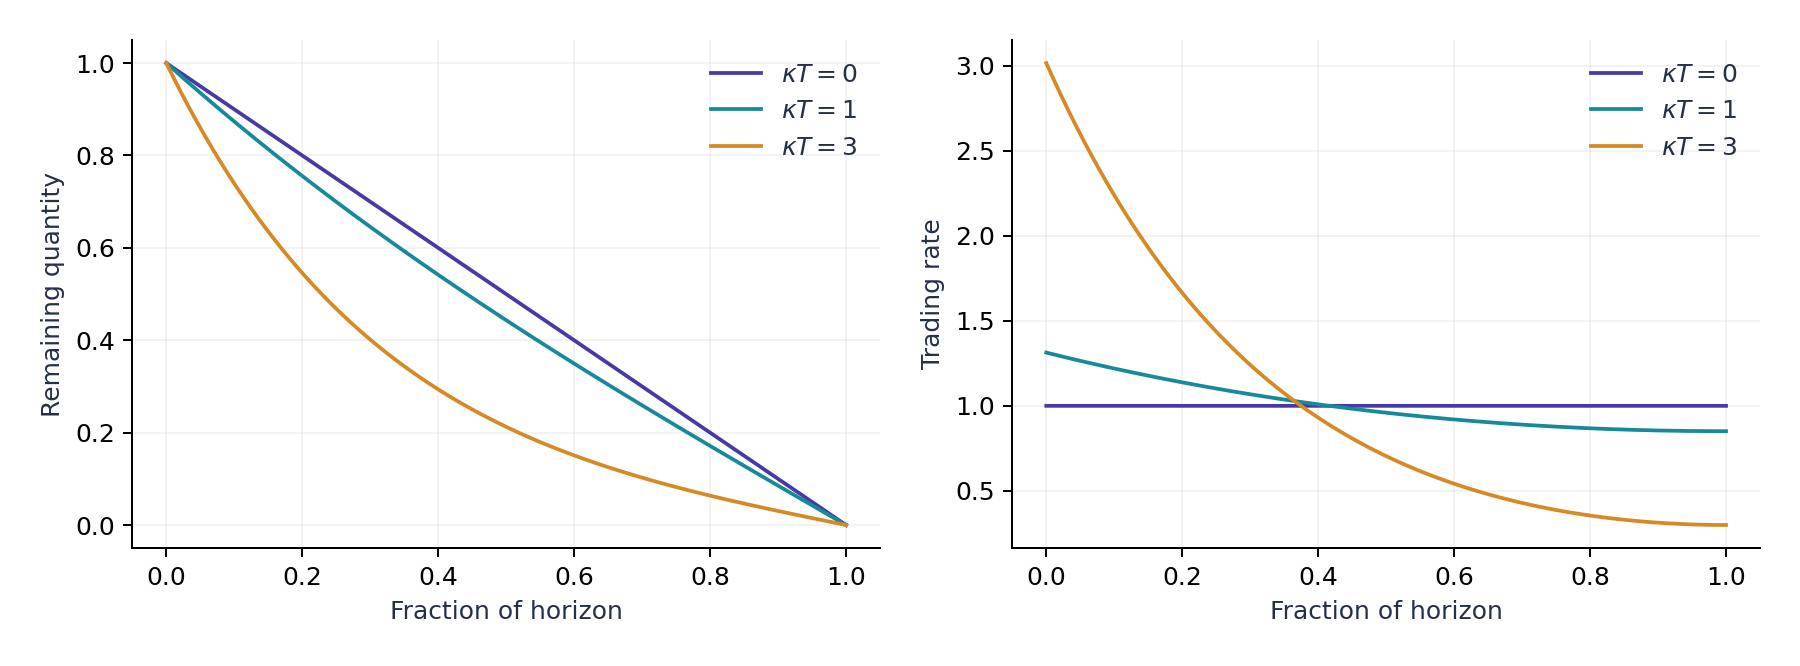
\includegraphics[width=\textwidth]{figures/01_schedules.png}
\caption{Analytic schedules with $Q=T=\eta=1$ and three values of $\kappa T$.
Greater exposure aversion moves execution earlier. These are deterministic
schedule calculations, not forecasts of available exchange liquidity.}
\label{fig:schedule}
\end{figure}

\subsection{Liquidity-dependent scheduling and feasibility}

For differentiable $\eta_t$ and an interior solution, the variational equation
becomes
\begin{equation}\label{eq:variable}
 (\eta_t\dot q_t)'=\lambda\sigma_t^2q_t+\frac12\alpha_t.
\end{equation}
Rate caps and monotonicity require constrained optimization rather than this
equation alone. On a discrete grid a convenient convex program is
\begin{align}\label{eq:discschedule}
 \min_{x_0,\ldots,x_{N-1}}\quad &
 \sum_k\left[C_k(x_k)+\lambda\sigma_k^2q_{k+1}^2\Delta t_k
                         +\alpha_kq_{k+1}\Delta t_k\right],\\[-3pt]
 \text{subject to}\quad &q_{k+1}=q_k-x_k,\quad
 0\leq x_k\leq\bar x_k,\quad q_0=Q,\quad q_N=0.\nonumber
\end{align}
For deterministic reliable capacities $\bar x_k$, feasibility is equivalent
to $Q\leq\sum_k\bar x_k$. Necessity follows by summing the capacities;
sufficiency follows by allocating greedily until $Q$ is exhausted.
Observed displayed depth is not a reliable future capacity: it can cancel
before the order arrives. In a stochastic model, hard guarantees must be
replaced by explicitly assumed capacity, a chance constraint, or a residual
mandate.

\subsection{Benchmarks are distinct objectives}

TWAP, VWAP, participation and implementation-shortfall algorithms are related
but not interchangeable. TWAP fixes a clock allocation. Forecast VWAP places
more volume in anticipated liquid intervals. Participation follows realized
activity and can lag a deadline. An arrival-price optimizer changes speed with
impact, drift and risk. An auction-focused strategy may concentrate at a
benchmark event. Benchmark tracking can be added through a term such as
$\theta\sum_k(q_k-\bar q_k)^2$, but this creates a different optimization
problem from minimizing arrival-price shortfall alone.

\part{Allocation, information and control}\label{pt:control}
\section{Joint allocation across venues}\label{sec:routing}

\subsection{Immediate liquidity and marginal cost}

Suppose a scheduler requests $x$ shares immediately and venue $v$ offers a
convex total cost $C_v(x_v)$ for taking $x_v\in[0,c_v]$. Costs include price
levels reached, specified impact and net fees, expressed relative to a common
reference. Define the effective cost
\begin{equation}\label{eq:infconv}
 C(x)=\min\left\{\sum_{v=1}^V C_v(x_v):
                 \sum_vx_v=x,\ 0\leq x_v\leq c_v\right\}.
\end{equation}
The problem treats $c_v$ as available at execution time. Price protection or
directed-order restrictions must be imposed when applicable; the simple box
formula below need not apply with additional routing constraints. Under latency, it is
an approximation conditional on those capacities; random availability belongs
in a stochastic extension.

\begin{theorem}[Convex venue aggregation]\label{thm:routing}
Let each $C_v$ be continuous and convex on $[0,c_v]$, with $c_v>0$.
For $0\leq x\leq\sum_vc_v$, the minimum in \eqref{eq:infconv} is attained and
$C$ is convex. If the costs are strictly convex, the allocation is unique.
For differentiable costs and an interior aggregate quantity, an optimum has
a multiplier $\mu$ satisfying
\begin{equation}\label{eq:kkt}
 \begin{cases}
 C_v'(x_v)=\mu,&0<x_v<c_v,\\
 C_v'(0)\geq\mu,&x_v=0,\\
 C_v'(c_v)\leq\mu,&x_v=c_v.
 \end{cases}
\end{equation}
Such a multiplier is a subgradient of $C$ at $x$; where $C$ is differentiable,
$C'(x)=\mu$.
\end{theorem}
\begin{proof}
The feasible set is nonempty and compact, so continuity gives attainment.
Take feasible optimizers for $x$ and $y$. Their convex combination is feasible
for $\theta x+(1-\theta)y$, and convexity of each cost bounds its objective
by $\theta C(x)+(1-\theta)C(y)$. This proves convexity of $C$. Strict convexity
rules out two distinct minimizing allocations. The multiplier conditions are
the first-order conditions for minimizing
$\sum_vC_v(x_v)-\mu(\sum_vx_v-x)$ over the box. Convexity makes them
sufficient; standard finite-dimensional multiplier conditions apply because
an aggregate quantity strictly between the endpoints admits a point interior
to every box interval. Finally, their supporting-line inequalities, summed
over venues, give $C(y)\geq C(x)+\mu(y-x)$.
\end{proof}

For $C_v(x)=a_vx+b_vx^2/2$, $b_v>0$, the solution is
\begin{equation}\label{eq:waterfill}
 x_v(\mu)=\clip\left(\frac{\mu-a_v}{b_v},0,c_v\right),\qquad
 \sum_vx_v(\mu)=x.
\end{equation}
This is a marginal-cost allocation, not a ranking by the smallest fee $a_v$.
A cheap venue may have rapidly increasing marginal cost or a binding capacity.
Piecewise-linear costs obtained by walking observed depth give the analogous
discrete allocation, with lot and price-grid constraints retained.

\begin{figure}[tb]
\centering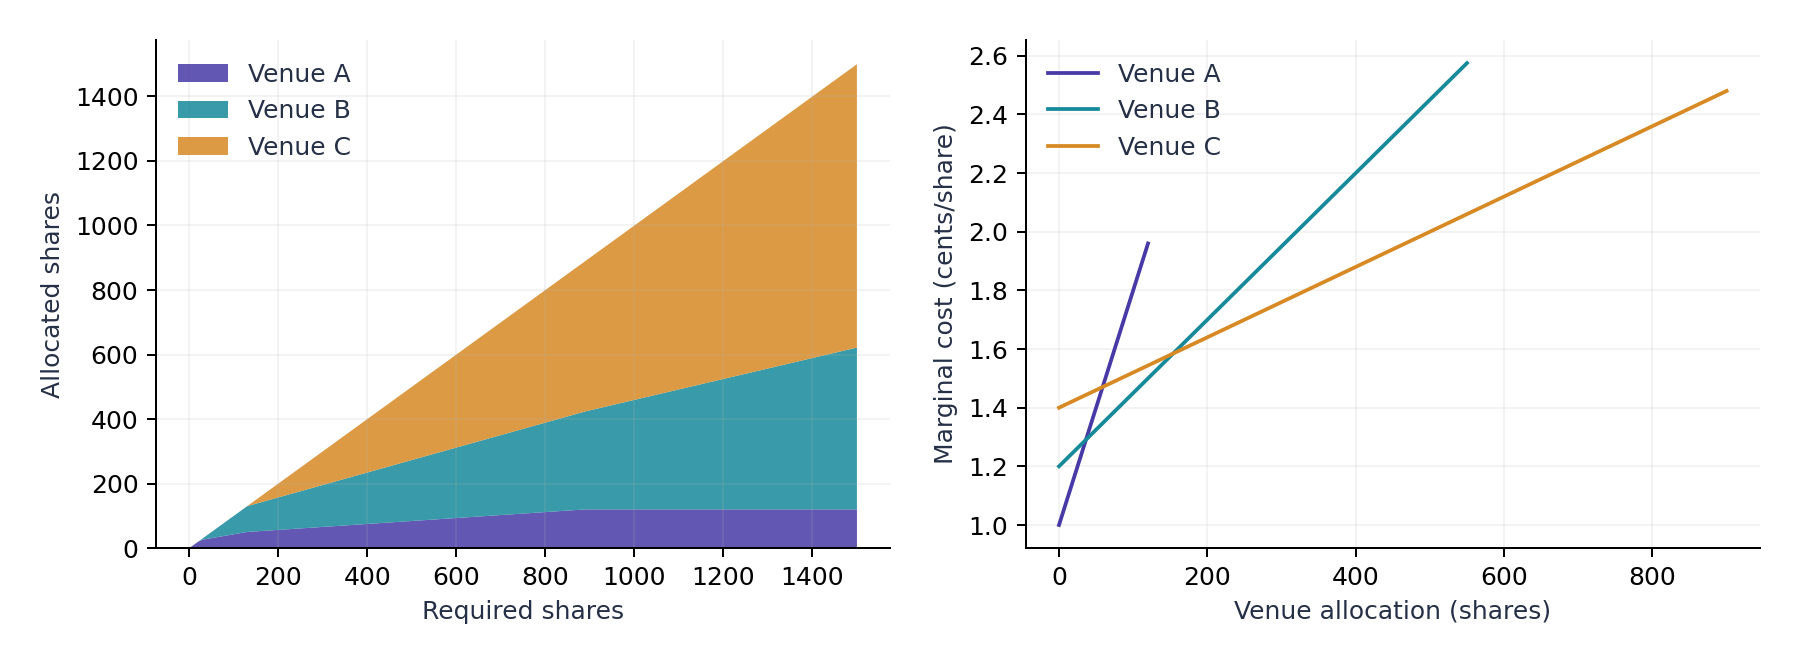
\includegraphics[width=\textwidth]{figures/02_routing.png}
\caption{Synthetic immediate allocation among three venues. The left panel
shows the allocation as required size increases. The right panel shows
marginal costs up to each venue's capacity. A venue with a low initial cost
need not receive most of a large parent slice.}
\label{fig:routing}
\end{figure}

\subsection{When decomposition is exact}

Substituting $C_k$ from \eqref{eq:infconv} into \eqref{eq:discschedule} preserves
convexity. This gives an exact schedule-then-route decomposition under three
specific assumptions: contemporaneous venue costs are separable; the chosen
allocation has no effect on future states beyond total executed quantity; and
all input states/capacities are specified independently of the allocation.
The scheduler uses the actual optimized venue cost, not an arbitrary average.

These assumptions fail when a route changes a queue, reveals hidden capacity,
creates venue-specific impact, or changes later fill dependence. Then the
correct routing comparison contains a continuation term,
\begin{equation}\label{eq:routecontinuation}
 \min_{a\in\A(q,s,b)}
 \E\left[c(s,a,Y)+V_{k+1}(q-F,s',b')\mid s,b,a\right].
\end{equation}
Two child-order choices with the same expected fill can have different values
because the variance and information in their fills differ.

\begin{example}[A schedule cannot ignore its effective cost]
There are two intervals, total quantity $1$, no risk, and effective costs
$C_1(x)=x^2$, $C_2(x)=9x^2$. A flat schedule $(1/2,1/2)$ costs $2.5$.
Minimizing $x^2+9(1-x)^2$ gives $(x_1,x_2)=(0.9,0.1)$ and cost $0.9$.
Routing optimally after committing to the flat schedule cannot recover the
lost timing decision. The example does not identify any actual exchange;
it shows the mathematical cost of imposing a schedule before modeling liquidity.
\end{example}

\subsection{Correlation and reservations}

Fill probabilities at different venues need not be independent. A common
price move, institutional sweep, or cancellation burst can affect all of them.
If two 80-share child orders are outstanding for a 100-share parent, each
having a 0.6 chance of full execution, independence gives a 0.36 probability
of a 60-share overfill and expected excess quantity $21.6$. The same marginal
probabilities permit joint full-fill probability anywhere between 0.2 and 0.6
by the Fr\'echet bounds. Marginals do not identify overfill risk.

One can penalize overfills in a stochastic allocation problem, as in the
broader placement literature \citep{cont2017}. A mandate that forbids them
instead needs a reservation constraint. Fast cancellation messages do not
create an atomic cancellation across independent venues.

\begin{proposition}[Reservation invariant]\label{prop:reserve}
Let $q$ be remaining parent quantity after authoritative reported fills.
For each outstanding child, reserve an upper bound $r_j$ on the additional
quantity it can execute that is not already included in those reported fills.
Reserve quantity before sending a new instruction. Maintain
\begin{equation}\label{eq:reservation}
 \sum_jr_j\leq q.
\end{equation}
Assume executions never exceed their child bounds, reported cumulative fills
are processed without duplication, and a cancellation releases a reservation
only when its terminal cumulative fill is authoritative. Then actual total
executions cannot exceed $Q$.
\end{proposition}
\begin{proof}
At each state, unreported and future executions on outstanding children sum
to at most $\sum_jr_j$. Previously reported executions equal $Q-q$.
Thus their combined upper bound is $Q-q+\sum_jr_j\leq Q$.
A new submission preserves the inequality by construction. An authoritative
partial fill of size $d$ decreases both $q$ and that child's bound by $d$.
A terminal cancellation removes only quantity that can no longer execute.
Induction over processed events preserves the invariant.
\end{proof}

Orders pending acceptance or cancellation still consume capacity if they may
execute. A replace may require reserving both old and new exposure until the
venue's atomic semantics are known. A disconnected route cannot be assumed
canceled. These facts belong in the state transition and in the optimizer's
action filter, not merely in a post-trade error report.

\section{Hidden liquidity and execution information}\label{sec:hidden}

\subsection{What is observed and what is inferred}

Let $H_t(p,v)$ be non-displayed resting liquidity and $R_t(p,v)$ iceberg reserve
at a fixed price and venue. Neither variable is the inventory held by a
financial institution. A dealer can hold a large position without offering
it for execution; a reserve order is a trading instruction, not a complete
balance sheet.

Displayed books, public prints, private fills, and order acknowledgments are
different observations of these latent states. Public data may be unable to
identify the hidden side or reserve identity. In Nasdaq's native non-cross trade
message, the order-reference field is zero and the buy/sell field is fixed to
\texttt{B}, irrespective of the resting side. Separate messages report cross
trades \citep{itch}. Neither the fixed side field nor an auction print identifies
continuous hidden buy liquidity. Message type and session state must be retained
before assigning uncertain sides or updating hidden-stock estimates.

A simple execution-count model illustrates non-identification:
\begin{equation}\label{eq:hiddenproduct}
 E_t\mid H_t,\kappa_t\sim\operatorname{Poisson}(\kappa_tH_t\Delta t).
\end{equation}
For $c>0$, replacing $(H_t,\kappa_t)$ by $(cH_t,\kappa_t/c)$ leaves this
likelihood unchanged. Counts identify an activity product, not the two factors
separately. Validated stock dynamics, multiple exposures, private information
or stronger assumptions are needed to learn more.

The Poisson likelihood is a reduced activity model, not a stock-conserving
execution law: it assigns positive probability to more executions than a fixed
finite starting stock. With integer $H_t$, no arrivals, replenishment, cancellations or other
competing exits, and independent per-share execution hazards, a compatible depletion law is instead
\[
 E_t\mid H_t,\kappa_t\sim
 \operatorname{Binomial}\!\left(H_t,1-e^{-\kappa_t\Delta t}\right),
 \qquad H_{t+1}=H_t-E_t.
\]
Its small-interval mean is approximately $\kappa_tH_t\Delta t$, but its full
likelihood does not retain the Poisson model's exact scaling invariance.
This does not identify a hidden stock from one observed count; inference still
depends on repeated observations, the hazard model, and assumptions about
arrivals, cancellation and replenishment.
Observed replenishment, cancellations and changing sides must enter the
transition jointly; clipping an independently sampled execution after the fact
changes the likelihood used for filtering.

The hidden-stock balance at a price should distinguish arrivals $A^H$,
cancellations $C^H$, executions $E^H$ and transfers. An iceberg balance uses
\begin{align}\label{eq:stock}
 D_{t+1}&=D_t+A^D_t-C^D_t-E^D_t+U_t,\\
 R_{t+1}&=R_t+A^R_t-C^R_t-E^R_t-U_t,\nonumber
\end{align}
where $U_t$ is replenishment into display. It cancels in the combined share
balance. Multiple such events can occur between two snapshots. The observed
endpoint does not determine their sequence, queue priority or gross turnover.

\begin{example}[A reserve transfer with residual priority]
For an explicitly assumed 100-share normal unit, start with 200 displayed
shares and 600 reserve shares. A 150-share execution leaves 50 displayed
shares. Replenishing with a new 200-share displayed clip leaves 400 in reserve.
The resulting 250 displayed shares comprise the old 50 and the new 200; their
timestamps differ. The ledger is $250+400+150=800$ shares. This scenario
illustrates the reserve rule; it does not infer the round lot or actual reserve
of any particular stock \citep{nasdaqrules}.
\end{example}

\subsection{Beliefs must condition on the trader's actions}

Let $s_t$ be observable state, $h_t$ latent state, and $b_t(h)$ its posterior
given the observation history and the trader's past instructions. With
transition $P(h'\mid h,s,a)$ and observation likelihood
$L(y\mid h',s,a)$, the next posterior is
\begin{equation}\label{eq:bayes}
 b_{t+1}(h')=
 \frac{L(y\mid h',s,a)\sum_hP(h'\mid h,s,a)b_t(h)}
 {\sum_{\tilde h}L(y\mid\tilde h,s,a)
              \sum_hP(\tilde h\mid h,s,a)b_t(h)}.
\end{equation}
Zero-probability observations require model repair or an explicit fallback,
not division by zero. A fill and a non-fill can both update liquidity beliefs.
Their informativeness depends on where, how much and how long the trader
posted. Private fills should not be treated as passive observations generated
independently of the policy.

In an event simulator, executed shares are realized outcomes. A model trained
on completed execution volume does not thereby learn unfilled aggressive
demand. Interpreting its output as a request and clipping it against a guessed
single-period reserve can manufacture enormous apparent non-fill rates.
Such a statistic diagnoses the combined simulator, not an actual market
rejection rate.

\subsection{Execution value without price-prediction value}

\begin{proposition}[A separation example]\label{prop:separation}
There exists an execution problem in which observing hidden liquidity strictly
reduces optimal expected execution cost while leaving every price forecast
unchanged.
\end{proposition}
\begin{proof}
Let a hidden regime $H\in\{0,1\}$ have equal prior probabilities. Let the
entire reference-price process be independent of $H$, for example a constant
price. One unit must be bought. Immediate execution costs $1$ relative to
the reference. Alternatively, submit a passive order that fills at cost zero
with probability $p_H$, where $p_0=0.1$ and $p_1=0.9$. Failure leads to
terminal completion at cost $2$. Conditional passive costs are $1.8$ and $0.2$.
Without regime information the passive expected cost is $1$, so the optimum
cost is $1$. With $H$ observed, execute immediately in regime 0 and passively
in regime 1, at mean cost $(1+0.2)/2=0.6$. The information saves $0.4$.
Independence implies that conditioning any price forecast on $H$ leaves its
distribution unchanged.
\end{proof}

This counterexample does not establish that hidden liquidity never predicts
prices. It establishes that predictive and execution value are different
properties. Conversely, a variable can affect real execution while its noisy
estimate adds no useful information beyond observed depth and flow. The
correct empirical question is whether a specified observation or estimate
improves a specified decision at a specified horizon.

\begin{figure}[tb]
\centering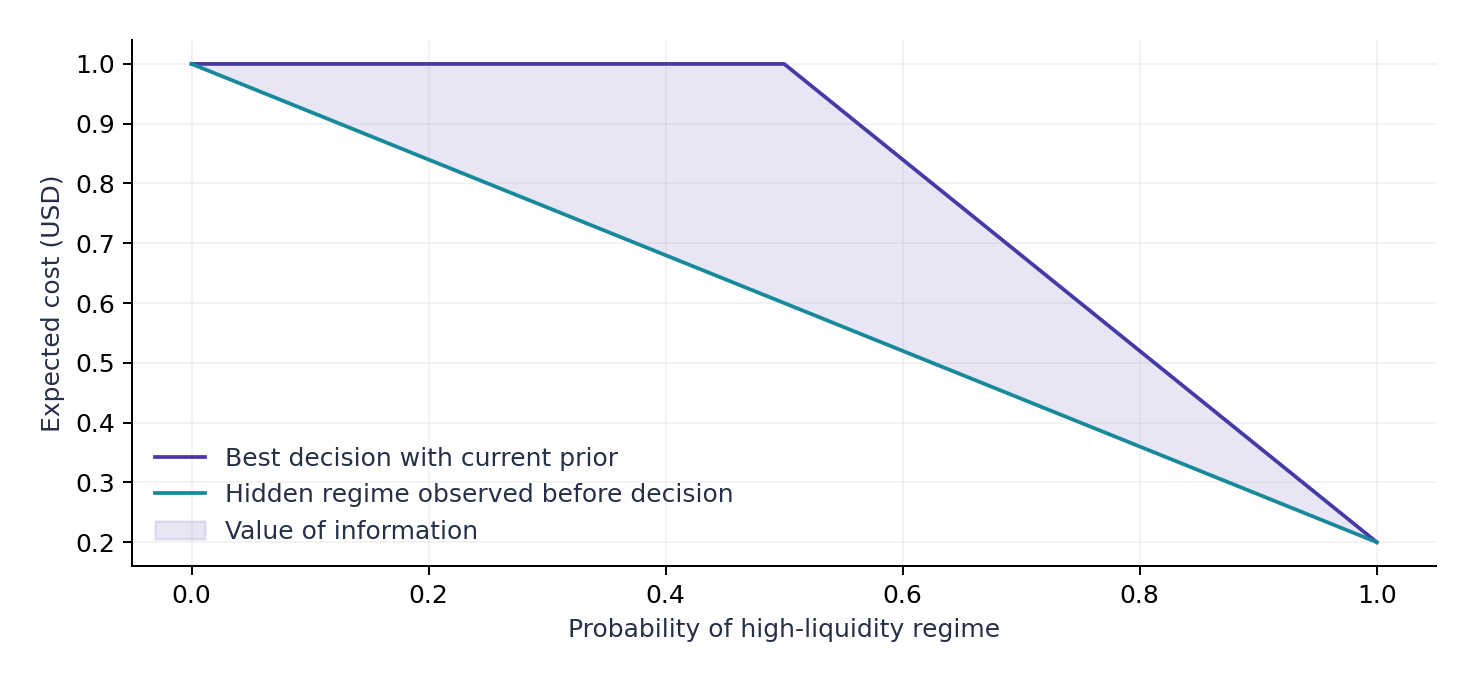
\includegraphics[width=.88\textwidth]{figures/04_information_value.png}
\caption{The exact information-value example of Proposition~\ref{prop:separation}
over different priors. The shaded gap is positive even though the price process
is independent of hidden regime. Information is assumed free and observed
before choosing the order.}
\label{fig:information}
\end{figure}

\section{From order flow and clearing to execution kernels}\label{sec:bookbridge}

A joint execution law can be constructed from primitive order arrivals,
cancellations and a matching rule. \citet{contdegondxuan2025} separate
stochastic order flow from deterministic clearing and factor the order-book
generator through these two operations. Their construction supplies the
starting point here. Execution control additionally needs order ownership,
priority, cash charges and private reports: two books with the same displayed
depth can give a particular trader different fills. This section retains
those marks, derives the joint kernel used in \cref{sec:dp}, obtains a
propagator as a stationary linear response, and carries primitive rate error
into a policy certificate.
Two further subsections make the resulting certificates computable:
Section~\ref{sec:computablepartial} encloses the partially observed optimum
for binary hidden liquidity, and Section~\ref{sec:summarycertificate}
certifies a controller that discards reports against the richer-history
optimum, in cost and in action.
The bounded finite-state assumptions are explicit;
the results do not assert a scaling limit or identify an empirical kernel.

\subsection{Clearing with ownership and a conserved parent ledger}

Fix a finite price grid and integer share units. At each price and side,
store an ordered queue of orders, retaining remaining size and an ownership
tag. Let $S$ be a finite structural state space containing these queues, the
parent residual $q$, live and pending own exposure, and any finite regime or
session variables needed to determine event rates and reports. Finite queue
capacities and a finite parent bound make this possible; continuous ages,
impact coordinates or latent variables require an explicitly stated finite
approximation if they are included in $S$. Accumulated cash and the full
report history can be recorded as additive marks outside $S$, provided future
rates and admissible actions do not require omitted information.

Consider first continuous matching under price--time priority. An arriving
buy consumes the lowest compatible sell price, oldest order first at that
price; a sell uses the highest compatible buy price. Each match removes the
minimum of the two remaining sizes and executes at the resting order's price.
An accepted limit-order residual joins the back of its queue; an
immediate-or-cancel residual expires. A cancellation names an existing order
and removes no more than its remaining size. Invalid requests and capacity
overflow have explicit rejection reports. Empty books remain possible: a
request cannot execute against depth absent from the state. These conventions
specify a deterministic map, including each trade and rejection, rather than
only a post-clearing depth vector.

Let $e$ be a primitive event mark and $a$ the current control mode. Write
\begin{equation}\label{eq:taggedclear}
 \mathfrak T^a(s,e)=\bigl(T^a(s,e),\omega^a(s,e)\bigr),
 \qquad T^a(s,e)\in S.
\end{equation}
The output $\omega$ contains the ordered trade list, own fills, execution
prices, fees and observable reports. A deterministic observation rule may
hide other participants' tags. Random hidden allocation or reporting can be
represented by enriching $e$ with the corresponding random mark. Atomic
decision-time messages use a separate map $\mathfrak I^a$ of the same kind.
Non-atomic messages instead enter the pending-message state and take effect
when their acknowledgment or execution events arrive.

\begin{proposition}[Clearing and parent conservation]\label{prop:taggedconservation}
Starting from an uncrossed book, the price--time construction terminates and
returns an uncrossed book with nonnegative queue sizes. Write $B^\pm$ for
total resting shares, $A^\pm$ for accepted arrivals, $C^\pm$ for cancellations,
$D^\pm$ for expired incoming residuals, and $V$ for matched volume during
one update. Then
\begin{equation}\label{eq:bookconservation}
 B^{\pm\prime}=B^\pm+A^\pm-C^\pm-D^\pm-V.
\end{equation}
For a buy-only parent, admit new potentially executable exposure only when
total live and pending own exposure $R$ remains at most $q$. If an own fill
of $F$ shares removes the same $F$ from $R$ and from $q$, and canceled
exposure is released only on an authoritative report, then $0\le R\le q$
is preserved. In particular, the parent cannot overfill. Its cash ledger
increments by $\sum_j f_jp_j+\mathrm{fees}$ and its residual by
$-\sum_jf_j$.
\end{proposition}
\begin{proof}
Every match exhausts the arriving residual or at least one finite resting
order. Thus the matching loop terminates. It leaves no compatible resting
counterparty for a residual that is posted, and a cancellation cannot create
a crossed book. Each match removes the same volume from the two sides;
arrivals, cancellations and expiry give \eqref{eq:bookconservation}.
An admitted instruction respects $R\le q$, a fill subtracts the same amount
from both sides of this inequality, and an acknowledged cancellation only
decreases $R$. Induction over messages and events proves the claim. The
cash and parent identities follow by summing the recorded own trades.
\end{proof}

This is a continuous price--time matching specialization. The NYSE parity,
reserve and auction mechanisms in \cref{sec:venues,sec:auctions} require
their own $\mathfrak T$, ownership categories and priority state. The
operator construction below remains applicable once that map is specified;
the FIFO example does not implement those additional rules.

\subsection{The controlled generator and the joint law}

Let $E$ be a finite mark set and let $\nu^a(s,e)\ge0$ be its primitive
event intensities. Assume, uniformly over admissible states and actions,
\begin{equation}\label{eq:bookrates}
 \lambda^a(s):=\sum_{e\in E}\nu^a(s,e)\le\Lambda,
 \qquad 0<\Lambda<\infty.
\end{equation}
The intensities may depend on own displayed orders, inventory, regime and
past activity retained in $s$. They are not required to be exogenous to
execution. At deterministic times $0=t_0<\cdots<t_N=T$, a policy chooses
an admissible action from its observed history; apply $\mathfrak I^a$ and
hold its control mode until the next decision. Finitely many interventions
exclude an accumulation of own messages at one time.

\begin{proposition}[A marked controlled book]\label{prop:bookgenerator}
The common bounded rate \eqref{eq:bookrates}, the event maps
\eqref{eq:taggedclear}, and the decision maps define a nonexplosive controlled
process and its joint execution/report law. Between decisions its state
generator, acting on functions $f:S\to\R$, is
\begin{equation}\label{eq:bookgenerator}
 (\mathscr L^a f)(s)=
 \sum_e\nu^a(s,e)\{f(T^a(s,e))-f(s)\}.
\end{equation}
For an additive event charge $c^a(s,e)$, the corresponding cost-plus-
continuation term is
\begin{equation}\label{eq:markedcostgenerator}
 \sum_e\nu^a(s,e)
 \{c^a(s,e)+f(T^a(s,e))-f(s)\}.
\end{equation}
State-preserving events can still carry a charge or a report and therefore
cannot in general be discarded from the marked model.
\end{proposition}
\begin{proof}
Use a Poisson clock of rate $\Lambda$. At a clock time in state $s$, draw a
mark from $E\cup\{\partial\}$ with probabilities
\begin{equation}\label{eq:bookuniformization}
 \mu_s^a(e)=\frac{\nu^a(s,e)}{\Lambda},\qquad
 \mu_s^a(\partial)=1-\frac{\lambda^a(s)}{\Lambda}.
\end{equation}
The dummy mark $\partial$ leaves state unchanged, has zero charge and gives
no observable report. Apply $\mathfrak T^a$ at every other mark. There are
almost surely finitely many clock times on $[0,T]$; the recursion therefore
constructs the process and all its marks. The probabilities of one and two
or more clock events in a short interval are $\Lambda\dd t+o(\dd t)$ and
$o(\dd t)$, respectively. Conditioning on the first mark gives
\eqref{eq:bookgenerator} and \eqref{eq:markedcostgenerator}.
\end{proof}

The state part is precisely the order-flow/clearing factorization. If
$R^a(s,e)$ denotes the intermediate raw update, $\mathcal C$ clears it,
$\widetilde{\mathcal C}f=f\circ\mathcal C$, and $\Xi$ restricts a function
to valid states, then $T^a=\mathcal C\circ R^a$, $\mathcal C(s)=s$ on
$S$, and
\begin{equation}\label{eq:bookfactorization}
 \mathscr L^a=\Xi\mathscr L_o^a\widetilde{\mathcal C}.
\end{equation}
On a valid state, the raw generator is
$\mathscr L_o^a g(s)=\sum_e\nu^a(s,e)\{g(R^a(s,e))-g(s)\}$;
any generator extension to the other raw states gives the same restricted
identity. The raw space retains the incoming-message data needed to determine
priority and the resting execution price. Substituting $f\circ\mathcal C$
in the raw generator proves \eqref{eq:bookfactorization}, following the
decomposition of \citet{contdegondxuan2025}. The additional marked
pushforward, rather than this state identity alone, provides the execution
ledger and observation likelihood.

For a fixed mode, let $P^a$ be the state transition matrix of one
uniformization clock. Its exact interval law is
\begin{equation}\label{eq:booksemigroup}
 e^{h\mathscr L^a}=
 e^{-\Lambda h}\sum_{n=0}^\infty
       \frac{(\Lambda h)^n}{n!}(P^a)^n.
\end{equation}
To retain cash and reports, compose the \emph{marked} updates along those
$n$ clock events before taking the desired marginal. Replacing the tail
$n>M$ by any declared fallback trajectory gives a probability law whose
total-variation distance from the exact interval law is at most
$\Pp\{\operatorname{Poisson}(\Lambda h)>M\}$. Clearing after every event
is essential: combining several arrivals before clearing can change own
priority, executions and reports.

Given the full state $s$, this construction produces a joint interval law
$\mathcal Q_k^a(s',y\mid s)$, with $y$ retaining the observed reports and
own trade records. If only a history $H_k$ is observed, let $b_k(s)$ be the
conditional distribution of the full state. Then
\begin{align}\label{eq:bookfilter}
 \K_k(s',y\mid H_k,a)&=\sum_s b_k(s)\mathcal Q_k^a(s',y\mid s),\\
 b_{k+1}(s')&=
 \frac{\sum_s b_k(s)\mathcal Q_k^a(s',y\mid s)}
 {\sum_{s,s''}b_k(s)\mathcal Q_k^a(s'',y\mid s)}.\nonumber
\end{align}
The posterior formula applies when the denominator is positive. Observable
state components are included in $y$; the corresponding inconsistent states
receive zero posterior mass. Marginalizing $\K_k$ gives the fills, price
records, next book, live orders and session variables in \cref{sec:dp}.
Thus the same matching calculation generates the fill distribution, its
associated prices, and the information used in the next decision.

A proposed reduced state $z=\rho(s)$ is sufficient if, whenever
$\rho(s_1)=\rho(s_2)$, both states have the same admissible actions and the
one-clock laws of $(\rho(s'),\omega)$ agree under each action. Induction
through \eqref{eq:booksemigroup} then gives a Markov control reduction; the
decision maps must obey the same condition. Aggregate displayed depth
usually fails this test. With one own unit $O$ and one external unit $E$
at the best bid, queues $(O,E)$ and $(E,O)$ have equal depth. One incoming
unit sell fills the parent only in the first queue. A reduced state must
retain priority information or a posterior over it.

\subsection{A propagator obtained from the book generator}

The full controlled book generally has neither a linear price response nor
a quadratic execution cost. A precise connection is available at a
stationary small-intervention limit. In this subsection take a finite
environmental book model, without a depleting parent inventory, with baseline
generator $L_0$ and stationary row distribution $\pi$. Let $m:S\to\R$ be
a bounded reference-price observable with an explicit convention for empty
sides. Consider the generator family
\[
 L_\epsilon(t)=L_0+\epsilon u(t)B,
 \qquad B\mathbf 1=0,
\]
where $u$ is a deterministic integrable signed input and this family consists
of valid generators for the amplitudes under consideration. It can arise by
differentiating primitive arrival intensities with respect to a trading
intervention while retaining a fixed clearing map. This is an assumption
about causal response, not a consequence of fitting an order-flow correlation.

\begin{proposition}[Stationary book response]\label{prop:bookresponse}
Start with distribution $\pi$, set $m_0=m-(\pi m)\mathbf1$, and let
$b=\lVert B\rVert_{\infty\to\infty}$. Then
\begin{align}\label{eq:bookresponse}
 \E_\epsilon[m(S_t)]-\pi m
 &=\epsilon\int_0^t G_{\rm book}(t-s)u(s)\dd s+R_\epsilon(t),\\
 G_{\rm book}(r)&=\pi B e^{rL_0}m_0,\nonumber\\
 |R_\epsilon(t)|&\le
 \frac{\epsilon^2 b^2\lVert m_0\rVert_\infty}{2}
                 \left(\int_0^t|u(s)|\dd s\right)^2.\nonumber
\end{align}
\end{proposition}
\begin{proof}
Let $U_\epsilon(0,t)$ be the inhomogeneous transition matrix. Variation of
constants gives
\[
 U_\epsilon(0,t)=e^{tL_0}
  +\epsilon\int_0^t U_\epsilon(0,s)u(s)B e^{(t-s)L_0}\dd s.
\]
Multiply by $\pi$ and $m_0$ and replace $U_\epsilon(0,s)$ in the integral
once by $e^{sL_0}$ plus its variation-of-constants remainder. Stationarity
gives the displayed first-order kernel. Every transition matrix is a
contraction in the supremum norm. The second-order remainder is bounded by
$\epsilon^2b^2\lVert m_0\rVert_\infty$ times
$\int_0^t|u(s)|\int_0^s|u(r)|\dd r\dd s$, which is one half of the
squared integral in \eqref{eq:bookresponse}.
\end{proof}

\begin{example}[An exact exponential response]\label{ex:bookexponential}
Let the reference-price state take values $-\Delta$ and $\Delta$. The upward
and downward transition rates are $\kappa+\epsilon\beta u(t)$ and
$\kappa-\epsilon\beta u(t)$, respectively, with $\kappa,\beta,\Delta>0$
and $|\epsilon\beta u(t)|\le\kappa$. Start from the symmetric stationary
law. Its mean $M(t)$ solves
\[
 M'(t)=-2\kappa M(t)+2\epsilon\beta\Delta u(t),\qquad M(0)=0.
\]
Consequently $G_{\rm book}(r)=2\beta\Delta e^{-2\kappa r}$ and the
convolution in \eqref{eq:bookresponse} is exact. This is a stipulated
two-state price model. It supplies an explicit exponential reduction, not a
claim that an arbitrary tagged book has two states or exponential resilience.
\end{example}

For a general finite generator, $\pi B e^{rL_0}m_0$ need not be a positive
mixture of exponentials: modal coefficients may have either sign, and
nonreversible dynamics can have nonreal modes. Thus round-trip
nonnegativity of the symmetric energy formed from this response remains a
separate condition in \cref{sec:linear,sec:defect}. Moreover, the proposition
concerns a mean price under deterministic intervention. Turning it into the
execution-cost energy requires additional assumptions about the own trade
process, the block convention and the reference-price ledger. It does not
justify replacing random action-dependent fills by their mean.

When $\omega$ already records realized execution prices from the book,
mechanical depletion is already in the cash ledger. Adding the cost generated
by the same fitted $G_{\rm book}$ would count that effect twice. A separate
impact coordinate must either replace a declared component of the price law
or represent an explicitly additional response, such as a shift of the
external reference price. Its effects on future event rates and observations
must then enter $\mathfrak T$ and $\nu$, as well as the cost convention.

\subsection{Primitive model error and execution regret}
\label{sec:primitivemodelerror}

Consider two models on the same full state, action and primitive-mark spaces,
with the same initial law, matching/report maps and decision-time maps. Let
their intensities be $\nu$ and $\widehat\nu$, both dominated by the common
clock $\Lambda$. Use the total-variation convention
$\TV(P,Q)=\sup_A|P(A)-Q(A)|$. Define
\begin{align}\label{eq:primitiveerror}
 \eta&=\sup_{s,a}\TV(\mu_s^a,\widehat\mu_s^a),\qquad d=\Lambda\eta,\\
 d&=\frac12\sup_{s,a}\left\{
       \sum_e|\nu^a(s,e)-\widehat\nu^a(s,e)|
       +|\lambda^a(s)-\widehat\lambda^a(s)|\right\}.\nonumber
\end{align}
The last term retains the difference in total event rates. Agreement of the
conditional event-type proportions alone is insufficient.

\begin{theorem}[From primitive rates to joint execution paths]\label{thm:bookcoupling}
For every common nonanticipating observed-history policy $\pi$, the two
joint laws of full state paths, own trades and observed reports through time
$t\le T$ satisfy
\begin{equation}\label{eq:bookpatherror}
 \TV(\mathbb P_\pi^{[0,t]},\widehat{\mathbb P}_\pi^{[0,t]})
       \le\beta_t:=1-e^{-dt}\le dt.
\end{equation}
In particular, a common deterministic matching/report map cannot increase
the one-clock primitive error $\eta$.
\end{theorem}
\begin{proof}
Use the same Poisson clock, initial full state and policy randomization.
While states and observed histories agree, the policy selects the same
action. Couple the two primitive marks maximally at each clock time. Their
conditional mismatch probability is at most $\eta$, uniformly over the
common state and action. A matched primitive mark has identical state,
execution and report outputs; identical interventions also preserve equality.
Conditional on $n$ clock times, the probability of no mismatch is at least
$(1-\eta)^n$. Averaging over the Poisson count gives at least
$e^{-\Lambda\eta t}$. The coupling inequality proves
\eqref{eq:bookpatherror}. The one-clock statement is the same argument with
a single mark, or the contraction of total variation under a pushforward.
\end{proof}

The policy in this theorem is the same map from observable history to
actions in both environments. In particular, a learned filter is held fixed
when evaluating the learned policy in the true environment. The theorem
does not require posterior distributions computed by the two different
models to be uniformly close after every rare observation. Such a
conditional claim would need extra assumptions. This direct full-path
coupling is therefore useful even when a uniform history-by-history
conditional bound of the form in \cref{prop:simulation} is unavailable.
If the initial full-state laws instead have total-variation distance
$\delta_0$, maximally coupling them first replaces $\beta_t$ by
$1-(1-\delta_0)e^{-dt}$.

If the matching or reporting maps differ, their discrepancy must also be
charged. For finite marks a sufficient one-clock replacement is
\begin{equation}\label{eq:clearingdisagreement}
 \eta_{\rm eff}=\min\!\left\{1,\sup_{s,a}\left[
 \TV(\mu_s^a,\widehat\mu_s^a)+
 \sum_e\widehat\mu_s^a(e)
       \mathbf1_{\{\mathfrak T^a(s,e)\ne\widehat{\mathfrak T}^a(s,e)\}}
                       \right]\right\}.
\end{equation}
Indeed, compare the pushforward of $\mu$ through $\mathfrak T$ first with
that of $\widehat\mu$ through the same map, then change the map.
Theorem~\ref{thm:bookcoupling} applies with $d=\Lambda\eta_{\rm eff}$
by coupling the joint outputs. Decision-time maps are still required to
agree; differences at deterministic interventions need their own coupling
error. Numerical truncation of \eqref{eq:booksemigroup} likewise contributes
its Poisson-tail probability. A finite capacity rule is an assumption of the
model, not an error-free approximation to unlimited depth.

\begin{corollary}[A combined execution certificate]\label{cor:bookcertificate}
Let $C(\omega)$ and $\widehat C(\omega)$ be the true and approximate total
loss functionals on a common feasible path space, with
\[
 \sup_\omega|C(\omega)-\widehat C(\omega)|\le D_{\rm cost}.
\]
Suppose $\widehat C$ lies in one common interval of width $L$ over all these
paths and policies. Then every fixed policy satisfies
\begin{equation}\label{eq:bookcosterror}
 |J_\pi-\widehat J_\pi|\le B_T,
 \qquad B_T=D_{\rm cost}+L(1-e^{-dT}).
\end{equation}
Let $\Pi_0\subseteq\Pi$ be a nonempty common feasible policy class and
let $\widehat\pi\in\Pi_0$ be $\tau$-optimal for the approximate objective
over $\Pi_0$. Then
\begin{equation}\label{eq:bookcertificate}
 J_{\widehat\pi}-\inf_{\pi\in\Pi}J_\pi
 \le 2D_{\rm cost}+2L(1-e^{-dT})+\tau+\Delta_{\Pi_0},
 \quad
 \Delta_{\Pi_0}=\inf_{\pi\in\Pi_0}J_\pi-\inf_{\pi\in\Pi}J_\pi.
\end{equation}
If the only same-path cost error is the single-asset quadratic impact term,
the grid and block convention of \cref{prop:impacttransfer}, together with
$\lVert x\rVert_1\le Q$ and entrywise kernel error $\varepsilon_K$, give
$D_{\rm cost}=Q^2\varepsilon_K/2$. The within-class bound becomes
\begin{equation}\label{eq:bookimpactcertificate}
 J_{\widehat\pi}-\inf_{\pi\in\Pi_0}J_\pi
 \le Q^2\varepsilon_K+2L(1-e^{-dT})+\tau.
\end{equation}
\end{corollary}
\begin{proof}
First change the pathwise loss on a fixed true trajectory, at cost at most
$D_{\rm cost}$. Then change its law while using $\widehat C$ on both sides.
The expectation of a function with range width $L$ changes by at most $L$
times total variation, proving \eqref{eq:bookcosterror}. Apply this bound to
$\widehat\pi$ and to an arbitrarily near-optimal member of $\Pi_0$, and
use approximate optimality between the two comparisons. Taking the infimum
and adding $\Delta_{\Pi_0}$ proves \eqref{eq:bookcertificate}. Finally,
$|x^\top(K-\widehat K)x|/2\le\varepsilon_K\lVert x\rVert_1^2/2$
gives \eqref{eq:bookimpactcertificate}.
\end{proof}

The range $L$ includes all approximate loss components, including variation
in impact cost across different fill paths. This matters when changing a
response model changes both prices and the distribution of fills. If its
cost decomposes into adapted stage losses of range widths $c_k$, realized by
$t_{k+1}$, the same proof sharpens the transition term to
$\sum_k c_k(1-e^{-dt_{k+1}})$. A bounded terminal charge can be included
in the final stage. Unbounded penalties or uncapped cumulative message fees
do not satisfy the stated bounded-loss hypothesis.

The impact norm and the transition metric are distinct hypotheses. A small
numerical change in a deterministically reported price can give disjoint
observation laws and total variation one. The same-path bound on
$\varepsilon_K$ therefore does not, by itself, supply a small $d$ for a
physically changed price or fill mechanism.

This construction also locates the scope of the signature certificate.
Finite signature features may parameterize an admissible history-feedback
class $\Pi_0$ in the controlled book, and \eqref{eq:bookcertificate} then
separates model error, optimization tolerance and class approximation.
However, the law of a book affected by those coefficients is endogenous.
The fixed moment matrix and exact quadratic objective in
\cref{thm:sigquadratic,thm:certificate} require their stated exogenous-path
assumption. They do not extend to this endogenous case merely by using
signature features. The book construction supplies the controlled law; a
separate argument is required for an exact reduced optimization objective.

\subsection{Feasible feedback policies and a vanishing class gap}
\label{sec:classgap}

The class term in \eqref{eq:bookcertificate} measures the restriction to a
chosen family of feasible feedback policies. A complete observable history
encoding and approximation in the laws induced by successive decisions give
a vanishing class gap. This result concerns the richness of the policy class;
the endogenous objective need not be quadratic or convex.

\begin{assumption}[Finite controlled book and observable feasibility]
\label{ass:finitebook}
Use the finite structural state and mark spaces of
\cref{prop:bookgenerator}, a common clock $0<\Lambda<\infty$, and $K\ge1$
deterministic decision times $0=t_0<\cdots<t_{K-1}<t_K=T$.
The action set $A$ is finite. At stage $k$ the nonempty admissible set
$A_k(H)\subseteq A$ is a Borel function of the trader's full observable
history. Its definition includes the ledger and terminal-feasibility
requirements; an absorbing completed state has a no-operation action.
The initial observation takes values in a finite alphabet. Each clock event
produces either no report or one finite-alphabet report bundle, and each
decision produces a finite-alphabet record of the chosen action and its
observable intervention output. A bundle retains the ordering of its
constituent reports and all observed ledger changes. The total loss $C$ is
measurable and lies in a common interval of width $L<\infty$ over feasible
paths and policies. All policies are behavioral probability kernels given
the observable history, including their own past actions.
\end{assumption}

Finite alphabets are explicit modeling restrictions on prices, sizes,
reports and initial observations. Finite structural states alone would not
imply a bounded total loss if, for example, uncapped message fees accumulated
at every clock event. Nonempty observable masks and admissible terminal
rules are also assumptions; a mask does not manufacture missing liquidity.

\subsubsection*{Replacing one decision at a time}

Write $\Pi$ for these feasible randomized policies and $J_\pi=\E_\pi C$.

\begin{lemma}[Policy perturbation]\label{lem:policyperturb}
For $\pi,\pi'\in\Pi$, let $\pi^{(j)}$ use
$\pi'_0,\ldots,\pi'_{j-1}$ followed by
$\pi_j,\ldots,\pi_{K-1}$, and put
\begin{equation}\label{eq:decisionmismatch}
 \delta_j=\E_{\pi^{(j)}}\left[
 \TV\bigl(\pi_j(\cdot\mid H_j),\pi'_j(\cdot\mid H_j)\bigr)\right].
\end{equation}
Under \cref{ass:finitebook},
\begin{equation}\label{eq:policyperturb}
 |J_\pi-J_{\pi'}|\le L\sum_{j=0}^{K-1}\delta_j.
\end{equation}
\end{lemma}
\begin{proof}
Consecutive hybrids have identical rules before $t_j$, so the law of $H_j$
is the law in \eqref{eq:decisionmismatch}. Couple their initial states,
clock events and primitive marks up to $t_j$, then couple their action
draws maximally conditional on $H_j$. Their later decision rules are the
same. Conditional on a matched action, the remaining paths, ledgers and
reports can therefore coincide. The full-path total variation is at most
$\delta_j$, so the expected losses differ by at most $L\delta_j$.
Sum from $\pi^{(0)}=\pi$ to $\pi^{(K)}=\pi'$.
\end{proof}

The histories in this lemma have the law generated by the already replaced
earlier decisions. Thus no likelihood-ratio comparison between different
policies, or continuity of the controlled value function, is required.

\subsubsection*{A complete observable history on a compact set}

Let $M_T$ count the uniformization clock events on $[0,T]$. Its law is
Poisson with mean $\Lambda T$, independently of which policy is used, and
\begin{equation}\label{eq:clocktail}
 \rho_n=\Pp\{M_T>n\}\downarrow0.
\end{equation}
The clock and its dummy marks are auxiliary objects, not observations used
by the policy. Encode only the actual observable transcript: first the
initial observation, then the timestamped report bundles and the trader's
own decision records, in their known order. Use a disjoint finite alphabet
$\mathcal B$ for these record types. Coincident timestamps retain their
record order. Immediately before decision $k$, the transcript has length
$m\le n+K+1$ on $\{M_T\le n\}$; the additional records account for the
initial observation and own interventions, which do not consume clock events.

For records $(\tau_i,b_i)_{i=1}^m$, with $\tau_1=0$ for the initial
observation, define the path $Z_k$ on $u\in[0,1]$ by linear interpolation
from the common origin through the $m$ nodes
\begin{equation}\label{eq:obslift}
 Z_k(0)=0,\qquad
 Z_k(i/m)=\left(i/m,\tau_i,\sum_{j=1}^i e_{b_j}\right),
 \quad 1\le i\le m.
\end{equation}
Here $e_b$ is the one-hot vector for record $b$. In particular $m\ge1$,
even when no clock report occurs. This encoding records a varying initial
observation as an increment from a fixed origin; it does not append it as
a constant coordinate. Policies and masks are Borel maps on the transcript
space; their values on impossible transcripts can be assigned arbitrarily.

\begin{lemma}[Compactness and separation of observable histories]
\label{lem:compacthist}
For fixed $n,k$, let $\mathcal H_{n,k}$ contain the lifts
\eqref{eq:obslift} with $1\le m\le n+K+1$, weakly ordered timestamps in
$[0,t_k]$, and letters in $\mathcal B$. This is compact in $1$-variation.
The lift is observable and injective on transcripts, every truncated
signature is continuous on $\mathcal H_{n,k}$, and signature-linear
functions are uniformly dense in $C(\mathcal H_{n,k})$.
\end{lemma}
\begin{proof}
For fixed $m$ and record string, the ordered timestamp simplex is compact.
Its interpolation map is continuous in $1$-variation: segment endpoints
vary continuously and the number and positions of interpolation segments
are fixed. There are finitely many such strings and lengths, so their
union is compact. All inputs are observed. The sum of the terminal record
coordinates recovers $m$; evaluating the path at $i/m$ then recovers each
timestamp and each one-hot record increment, proving injectivity.
All paths start at zero, and the strictly increasing first coordinate $u$
removes tree-like ambiguity. Signature uniqueness and the shuffle algebra
therefore give separation and Stone--Weierstrass density, exactly as in
\cref{thm:siguniversal}; continuity follows in the $1$-variation topology.
\end{proof}

Finite observable summary coordinates can also be appended when their node
values are determined by the discrete record string. This preserves
compactness and separation. For a fully observed finite book, one example
is the one-hot current state at each record node, starting at zero before
the initial record. Its first-level signature is the current state indicator.
Such a channel is unavailable when that state is hidden. In general the
index parameterization is part of the specified encoding: signature
invariance under reparameterization does not justify dropping record order,
initial information, or the trader's own decisions.

\subsubsection*{Approximation of scores with an exact admissibility mask}

For a nonempty mask $B\subseteq A$, write $\sigma_B(g)$ for the softmax
of finite scores $g\in\R^{|A|}$ restricted to $B$, with zero probability
outside $B$. Along $g+t(h-g)$ its derivative is
$p_a\{(h_a-g_a)-\sum_b p_b(h_b-g_b)\}$, and hence
\begin{equation}\label{eq:maskedlipschitz}
 \TV\bigl(\sigma_B(g),\sigma_B(h)\bigr)
 \le \min\{1,\|g-h\|_\infty\}.
\end{equation}
This estimate compares scores at one fixed history and its common mask;
it does not require the mask to vary continuously between histories.

Let $\Pi^N$ consist of policies
\begin{equation}\label{eq:sigsoftmax}
 \pi_k^\ell(a\mid H_k)=
 \frac{\mathbf1_{\{a\in A_k(H_k)\}}
  \exp\langle\ell_{k,a},\mathbb S^{\le N}(Z_k)\rangle}
 {\sum_{a'\in A_k(H_k)}
  \exp\langle\ell_{k,a'},\mathbb S^{\le N}(Z_k)\rangle}.
\end{equation}
Nonempty masks make the denominator positive. Every such policy is
observable and feasible, and $\Pi^N\subseteq\Pi^{N+1}$ by zero padding.
Coefficients are finite but have no common norm cap.

\begin{theorem}[Vanishing feasible signature class gap]\label{thm:classgap}
Under \cref{ass:finitebook}, with the complete encoding
\eqref{eq:obslift},
\begin{equation}\label{eq:classgap}
 0\le\Delta_{\Pi^N}:=\inf_{\pi\in\Pi^N}J_\pi-
             \inf_{\pi\in\Pi}J_\pi\downarrow0.
\end{equation}
More precisely, for every $\epsilon>0$, integer $n\ge0$, $\delta>0$,
$\alpha\in(0,1)$ and $b>0$, there are a finite depth $N$ and a policy in
$\Pi^N$ such that
\begin{equation}\label{eq:classgapbudget}
 \Delta_{\Pi^N}\le\epsilon+KL(\rho_n+\delta+\alpha+b).
\end{equation}
The depth is existential; the stated hypotheses supply no uniform
depth-versus-error or coefficient-norm bound.
\end{theorem}
\begin{proof}
Fix an $\epsilon$-optimal feasible policy $\pi$. Construct its replacement
forward, one stage at a time. At stage $k$, earlier replacement rules are
already fixed. On $\mathcal H_{n,k}$ use the finite Borel subprobability
measure
\[
 \zeta_k(D)=\Pp_{\pi^{(k)}}\{Z_k\in D,\ M_T\le n\}.
\]
Conditioning a measure on this auxiliary event introduces no future
information into the implemented rule, which remains a function of $Z_k$.

First floor the target distribution only on its admissible actions:
$p_k^\alpha=(1-\alpha)\pi_k+
\alpha\,\mathrm{unif}(A_k(H))$. Define real-valued scores on every action by
\[
 g_{k,a}(H)=
 \begin{cases}
  \log p_k^\alpha(a\mid H),&a\in A_k(H),\\
  0,&a\notin A_k(H).
 \end{cases}
\]
These are bounded Borel functions in $[\log(\alpha/|A|),0]$, and
$\sigma_{A_k(H)}(g_k(H))=p_k^\alpha(\cdot\mid H)$ exactly.
In particular no logarithm of zero is taken.

Apply Lusin's theorem to the finite vector $g_k$ under $\zeta_k$. There
is a compact $F_k\subseteq\mathcal H_{n,k}$ with
$\zeta_k(\mathcal H_{n,k}\setminus F_k)\le\delta$ on which all its
coordinates are continuous. By the bounded Tietze extension theorem each
coordinate extends continuously to $\mathcal H_{n,k}$. The extensions are
scores, so they need not satisfy a varying probability-simplex constraint.
By \cref{lem:compacthist}, approximate all extended scores by
signature-linear functions with uniform error at most $b$, using some
finite stage depth $N_k$. Masking their softmax gives a feasible rule
$\pi'_k$ on every history, including histories outside this compact set.

On $F_k$, flooring changes the target by at most $\alpha$ in total
variation, and \eqref{eq:maskedlipschitz} adds at most $b$. On its complement
total variation is at most one. Thus the mismatch in
\eqref{eq:decisionmismatch} obeys
$\delta_k\le\rho_n+\delta+\alpha+b$. Continue to the next stage under
the law generated by the replacement rules already fixed. At the end take
$N=\max_k N_k$ and zero-pad the coefficients, which changes none of these
rules or laws. \Cref{lem:policyperturb} and $\epsilon$-optimality give
\eqref{eq:classgapbudget}. Let $n\to\infty$ and
$\epsilon,\delta,\alpha,b\downarrow0$. Nestedness then proves
\eqref{eq:classgap} for the full sequence of depths.
\end{proof}

The admissibility mask can be discontinuous. For example, if only $a$ is
allowed for a scalar history coordinate $h\le1/2$ and only $b$ for $h>1/2$,
there is no globally continuous feasible probability vector. The proof
above extends finite scores on a large compact set and retains the mask
exactly, so it does not require such a vector. Initial information is
equally essential: with an observed fair bit $B$ and loss
$\mathbf1_{\{a\ne B\}}$, an encoding that omits $B$ has infimum $1/2$
while the unrestricted observed-history infimum is zero. The initial token
in \eqref{eq:obslift} excludes this failure.

\begin{corollary}[Conditional convergence of the combined certificate]
\label{cor:convergence}
Fix one true controlled book and loss. Let approximate models share its
state and action spaces, initial law, decision and report maps, history
encoding, and observable admissibility masks, as required in
\cref{cor:bookcertificate}. Suppose the true and approximate losses have
uniformly bounded range width $L$, and use a common $\Lambda,K$.
Let $\widehat\pi_j\in\Pi^{N_j}$ have global approximate-objective gap at
most $\tau_j$ within that class. If
$d_j,D_{{\rm cost},j},\tau_j\to0$ and $N_j\to\infty$, then
\begin{equation}\label{eq:convergence}
 J_{\widehat\pi_j}-\inf_{\pi\in\Pi}J_\pi\longrightarrow0.
\end{equation}
For an impact-only same-path error with entrywise kernel error
$\varepsilon_{K,j}$ and gross volume at most $Q$, the error decomposition is
\begin{equation}\label{eq:convergencerate}
 J_{\widehat\pi_j}-\inf_{\pi\in\Pi}J_\pi
 \le Q^2\varepsilon_{K,j}+2L(1-e^{-d_jT})+\tau_j
                         +\Delta_{\Pi^{N_j}}.
\end{equation}
\end{corollary}
\begin{proof}
The common encoding and masks give the same feasible class in both models.
Apply \eqref{eq:bookcertificate} and then \cref{thm:classgap} to the fixed
true objective. Each term vanishes under the stated hypotheses.
\end{proof}

This is a consistency statement conditional on global optimization
tolerances, not an algorithm establishing them. Even a one-decision
two-action softmax with costs $0$ and $1$ gives
$J(\ell)=(1+e^{-\ell})^{-1}$, whose second derivative changes sign.
Endogenous signature-softmax optimization is therefore not generally
convex. A local optimizer's stationarity residual cannot be substituted for
$\tau_j$. Nor does \eqref{eq:classgapbudget} make its Lusin defect and
depth choice empirically estimable without further regularity and
statistical assumptions. Fixed coefficient caps would define a different
class and require a separate approximation argument.

\begin{proposition}[An explicit finite-state softmax approximation]
\label{prop:finitesoftmax}
In a fully observed finite-state Markov specialization with additive stage
and terminal losses and a deterministic optimal policy $a_k^*(s)$, append the observable current-state
indicator channel described after \cref{lem:compacthist}. Set its depth-one
logit for $a_k^*(s)$ to $r\ge0$, and every other admissible logit to zero.
For $m_A=|A|$, the resulting policy $\pi^r$ satisfies
\begin{equation}\label{eq:finitesoftmax}
 0\le J_{\pi^r}-J^*
 \le\min\left\{L,\ KL\frac{m_A-1}{e^r+m_A-1}\right\}.
\end{equation}
\end{proposition}
\begin{proof}
Finite backward induction supplies $a_k^*$. With $m\le m_A$ admissible
actions, its selection probability is $e^r/(e^r+m-1)$; the total variation
from the deterministic rule is at most $(m_A-1)/(e^r+m_A-1)$.
Apply \cref{lem:policyperturb}; the common loss range supplies the cap $L$.
The indicator channel's endpoint is a first-level signature coordinate,
so stage- and state-specific logits have exactly the claimed depth.
\end{proof}

This construction requires a finite-state optimization oracle and an
observed state. Its explicit approximation parameter is the logit size $r$,
not increasing depth. It gives a computable $\tau$ bound for the numerical
specialization below; it does not provide a depth rate for the general
partially observed transcript model.

\subsection{Reference models and the price of an exogenous approximation}
\label{sec:endodefect}

The reference model must be specified as a complete controlled law before
it can be compared with the true book. Calling a fixed action a reference
mode does not establish that its feature process is exogenous.

\begin{proposition}[Reference-model defect and surrogate regret]
\label{prop:endodefect}
Let $\mathbb P_\pi$ and $\mathbb P^0_\pi$ have a common initial law,
clock bound, full state and action spaces, and common feasible
observed-history policies. Allow different marked event maps. Define
\begin{equation}\label{eq:feedbackgain}
 \gamma=\min\!\left\{1,\sup_{s,a}\left[
  \TV(\mu_s^a,\mu_s^{0,a})+
  \sum_{e\in E\cup\{\partial\}}\mu_s^{0,a}(e)
   \mathbf1_{\{\mathfrak T^a(s,e)\ne\mathfrak T^{0,a}(s,e)\}}
                         \right]\right\}.
\end{equation}
At decision $k$, suppose the two joint intervention-output laws, given
the same state and action, have total variation at most $\kappa_k$.
Identical decision maps have $\kappa_k=0$. Put
\[
 \beta_0=1-e^{-\Lambda\gamma T}\prod_{k=0}^{K-1}(1-\kappa_k).
\]
For losses with $\sup_\omega|C(\omega)-C^0(\omega)|\le D_0$ and
$C^0$ in one interval of width $L$, every fixed policy satisfies
\begin{equation}\label{eq:endodefect}
 |J_\pi-J^0_\pi|\le D_0+L\beta_0.
\end{equation}
For a common feasible coefficient family $\pi^\ell$, $\ell\in\mathcal L$,
let a computable surrogate $F$ satisfy
$\sup_{\ell\in\mathcal L}|F(\ell)-J^0_{\pi^\ell}|\le D_{\rm red}$.
If $\widehat\ell$ is globally $\tau$-optimal for $F$ over $\mathcal L$, then
\begin{equation}\label{eq:endocertificate}
 J_{\pi^{\widehat\ell}}-\inf_{\ell\in\mathcal L}J_{\pi^\ell}
 \le 2D_0+2L\beta_0+2D_{\rm red}+\tau.
\end{equation}
\end{proposition}
\begin{proof}
The one-clock output comparison is \eqref{eq:clearingdisagreement}.
While the coupled paths agree, the probability of retaining agreement at
an intervention is at least $1-\kappa_k$. Conditional on $n$ clock events,
multiply these bounds with $(1-\gamma)^n$ and average the Poisson count.
The full-path mismatch probability is at most $\beta_0$.
Change first the pathwise cost and then its law to obtain
\eqref{eq:endodefect}. The uniform difference between $J_{\pi^\ell}$ and
$F(\ell)$ is at most $D_0+L\beta_0+D_{\rm red}$.
Apply it to $\widehat\ell$ and to any near-minimizer of the true objective,
inserting the global $\tau$-optimality inequality between them.
\end{proof}

With identical interventions, the same loss, and an exact reduced reference
objective, this becomes $2L(1-e^{-\Lambda\gamma T})+\tau$.
Zero $\gamma$ is a sufficient agreement condition for positive-probability
clock outputs at a common state. It is not a characterization of
policy-independent feature laws, nor is this primitive upper bound
necessarily zero whenever two different primitive representations have the
same output law. Intervention discrepancies and reduction error cannot be
discarded.

\begin{example}[Freezing a mode can leave an endogenous feature law]
\label{ex:modefreezing}
Take $S=\{0,1\}$ and $A=\{0,1\}$. The decision at time zero sets
$s=a$. A state-preserving report event has rate $1+s$ and reports the
current state. At a fixed state these intensities and event maps do not
depend on the action label, so replacing that label by $a_0=0$ gives
$\gamma=0$. Retaining the same decision map nevertheless gives
\[
 \Pp_a\{\hbox{at least one report by }T\}=1-e^{-(1+a)T}.
\]
Thus the reference feature law still depends on the selected action.
The coupling comparison correctly gives equality of true and reference
costs for each fixed policy; it does not assert equality across policies.
If the reference intervention also resets the state to zero for every
action, its discrepancy for action one must instead be charged through
$\kappa_0=1$. The report indicator is a bounded loss, so this example
does not rely on an unbounded fee or queue.
\end{example}

A sufficient condition for an exogenous reference feature process is an
autonomous observable projection. Specifically, suppose a projection
$Y=\rho(s)$ has, at every reference clock event, a joint law of its next
value and its external feature reports that depends only on $Y$, not on
the own-order coordinates or chosen action. Suppose reference
interventions preserve $Y$ and emit no action-dependent feature reports,
and the initial projected law is fixed. Induction along the common clock
and decision times then proves that the projected feature history has a
policy-independent law. Any prescribed nonanticipating continuous
finite-variation transform of that history has the same independence.
The feature process must be maintained on the fixed horizon even after
parent completion; stopping it at a policy-dependent completion time would
generally reintroduce dependence.

To set $F(\ell)=\ell^\top Q\ell+b^\top\ell+\mathrm{const}$ and
$D_{\rm red}=0$, one must additionally establish the rate-policy, cost,
moment and common-feasibility assumptions of
\cref{thm:sigquadratic,thm:completion}. Autonomous external prices alone
do not make queue-dependent passive fills a quadratic rate cost. If that
identity is only approximate, its uniform objective discrepancy belongs in
$D_{\rm red}$. These conditions state exactly when the exogenous quadratic
programme has a transferable guarantee; the controlled-book class-gap
argument does not require them.

\begin{remark}[Scope of the approximation result]\label{rem:scopelimits}
The bounded clock supplies the uniform Poisson tail, finite records supply
compact transcript sets, nonempty observable masks supply exact feasibility,
and the bounded loss converts mismatch probability to objective error.
Unbounded arrival rates, infinite record alphabets and unbounded penalties
require separate tightness or integrability arguments. No extension to
those cases, no general depth complexity, and no empirical identification
guarantee is asserted by \cref{thm:classgap,cor:convergence}. The finite-state
illustration supplies a computable special case under its declared oracle
and observability assumptions.
\end{remark}

\subsection{Computable certificates under partial observation}
\label{sec:computablepartial}

The class gap in \cref{thm:classgap} is existential. A finite-observation
specialization admits a different, constructive route: compute a lower bound
on the unrestricted partially observed optimum and an upper bound on the
cost of an implementable controller. Their difference is a global certificate.
Belief-state dynamic programming and its piecewise-linear value functions are
classical \citep{smallwood1973}; computable bounds and finite-horizon
point-based planning are developed by \citet{lovejoy1991} and
\citet{walravenspaan2019}. The construction below combines those foundations
with the execution ledger, an observable finite-memory signature policy, and
the model-error certificate of \cref{cor:bookcertificate}.

\begin{assumption}[Finite observations and a binary hidden state]
\label{ass:finiteobservation}
There are $K$ decision stages, a finite observable state space $\mathcal X$,
a hidden state $h\in\{0,1\}$, and finite action and observation alphabets.
The nonempty feasible set $A_k(x)$ depends only on the observable state,
which retains every ledger, reservation and session variable needed for
feasibility. The joint controlled kernel is
\[
 M_{k,x,a,o}(h,h')\ge0,\qquad
 \sum_{o,h'}M_{k,x,a,o}(h,h')=1.
\]
An outcome $o$ determines the next observable state $x'=F_k(x,a,o)$ and
the stage charge $c_k(x,a,o)$. A terminal charge $c_K(x,h)$ is allowed.
Actions may change both the hidden transition and the observation law.
For each stage $j$, all remaining total losses lie in a common interval of
width $S_j$ over states and feasible continuation policies. All primitive
arrays, charges and these bounds are supplied. The initial state $x_0$ and
belief $b_0=\Pp(h_0=1)$ are known.
\end{assumption}

The analytic statements allow real data. Algorithmic claims require rational
primitives and grid nodes, or validated enclosures together with certified
comparisons for the controller's memory update.

The observation alphabet is the information actually available to this
controller. If a marked continuous-time model is reduced to these symbols,
discarding timestamps or reports changes the information problem unless
sufficiency is proved. No equivalence with a richer observation filtration
is assumed. Section~\ref{sec:summarycertificate} supplies a separate
certificate for that richer comparison. Binary hidden liquidity is the explicit computable case below;
it does not exhaust the finite hidden-state setting.

For $b\in[0,1]$, put $\boldsymbol b=(1-b,b)$ and define
\begin{align}\label{eq:finitebeliefkernel}
 p_b^a(o)&=\sum_{h,h'}\boldsymbol b_h M_{k,x,a,o}(h,h'),&
 \Phi_b^a(o)&=\frac{\sum_h\boldsymbol b_h M_{k,x,a,o}(h,1)}{p_b^a(o)},\\
 r_k(x,b,a)&=\sum_o p_b^a(o)c_k(x,a,o).\nonumber
\end{align}
Zero-probability outcomes contribute zero and may be assigned any posterior.
The optimal value $V_k(x,b)$ minimizes expected remaining cost over all
policies using the declared observation history, including their own actions.

\begin{lemma}[Concavity and a computable belief modulus]\label{lem:beliefmodulus}
For fixed $k,x$, $V_k(x,\cdot)$ is concave, piecewise linear and
$S_k$-Lipschitz on $[0,1]$.
\end{lemma}
\begin{proof}
A fixed deterministic continuation tree has conditional costs $v_0,v_1$,
so its expected cost is $(1-b)v_0+bv_1$. The common feasible action masks
give the same finite family of trees for every $b$. Their minimum is concave
and piecewise linear. The range assumption gives $|v_1-v_0|\le S_k$ for
every tree; taking minima preserves that Lipschitz bound. Behavioral
randomization cannot improve the minimum of these expected costs.
\end{proof}

\subsubsection*{Two finite backward recursions}

Let $G_m=\{0,1/m,\ldots,1\}\cup\{b_0\}$, and let $Q_m b$ be a
nearest node, with a fixed tie rule. Write $I_m f$ for linear interpolation
of node values: if $b=(1-\theta)g_i+\theta g_{i+1}$, then
$(I_m f)(b)=(1-\theta)f(g_i)+\theta f(g_{i+1})$.
Adjacent nodes have distance at most $1/m$; inserting the initial prior
therefore preserves the mesh estimates without restricting its value.
The nearest-node planning problem is the finite Markov decision process
\begin{align}\label{eq:nearestbeliefdp}
 W_K(x,g)&=(1-g)c_K(x,0)+g\,c_K(x,1),\nonumber\\
 W_k(x,g)&=\min_{a\in A_k(x)}\left\{
 r_k(x,g,a)+\sum_o p_g^a(o)
 W_{k+1}\bigl(F_k(x,a,o),Q_m\Phi_g^a(o)\bigr)\right\}.
\end{align}
Let $a_k^m(x,g)$ be a minimizing action. Independently compute
\begin{align}\label{eq:belieflowerdp}
 \underline V_K^m(x,g)&=(1-g)c_K(x,0)+g\,c_K(x,1),\nonumber\\
 \underline V_k^m(x,g)&=\min_{a\in A_k(x)}\left\{
 r_k(x,g,a)+\sum_o p_g^a(o)
 (I_m\underline V_{k+1}^m)\bigl(F_k(x,a,o),\Phi_g^a(o)\bigr)\right\}.
\end{align}
Interpolation here gives a lower relaxation for cost minimization. It is
not the deployed controller's state update.

The deployed controller starts at $\gamma_0=b_0$, selects
$a_k^m(x_k,\gamma_k)$, and updates its observable memory by
\begin{equation}\label{eq:beliefmemory}
 \gamma_{k+1}=Q_m\Phi_{\gamma_k}^{a_k}(o_{k+1}).
\end{equation}
This recursively rounded belief need not equal the true posterior conditional
on the entire observed history. The physical hidden state always evolves
according to $M$; it is never redrawn from $\gamma_k$ in deployment.

\subsubsection*{Evaluation in the physical model}

For any feasible finite-memory action probabilities $\sigma_k(a\mid x,\gamma)$
and the update \eqref{eq:beliefmemory}, evaluate on the augmented state
$(x,\gamma,h)$:
\begin{align}\label{eq:truecontrollerevaluation}
 E_K(x,\gamma,h)&=c_K(x,h),\nonumber\\
 E_k(x,\gamma,h)&=\sum_{a\in A_k(x)}\sigma_k(a\mid x,\gamma)
 \sum_{o,h'}M_{k,x,a,o}(h,h')\bigl\{c_k(x,a,o)\nonumber\\
 &\hspace{23mm}+E_{k+1}\bigl(F_k(x,a,o),Q_m\Phi_\gamma^a(o),h'\bigr)\bigr\},\\
 U_m(\sigma)&=(1-b_0)E_0(x_0,b_0,0)+b_0E_0(x_0,b_0,1).\nonumber
\end{align}
The hidden coordinate is integrated out offline. Neither the online action
nor its memory update observes $h$. Evaluation may also use a different
physical kernel while retaining the planner's filter in the memory update.

\begin{theorem}[A computable global execution certificate]
\label{thm:computablepartial}
Under \cref{ass:finiteobservation}, write $V^*=V_0(x_0,b_0)$. For every
feasible controller evaluated by \eqref{eq:truecontrollerevaluation},
\begin{equation}\label{eq:computablegap}
 \underline V_0^m(x_0,b_0)\le V^*\le U_m(\sigma),\qquad
 0\le J_\sigma-V^*\le
 \mathcal G_m(\sigma):=U_m(\sigma)-\underline V_0^m(x_0,b_0).
\end{equation}
All quantities on the right are obtained by finite backward induction.
An outward lower enclosure of $\underline V_0^m$ and outward upper enclosure
of $U_m$ give a valid numerically enclosed certificate. The result holds
for any candidate table; its validity does not require a local optimizer
to have found a global minimum.
\end{theorem}
\begin{proof}
At $K$ the grid terminal values are exact. If
$\underline V_{k+1}^m(x,g_i)\le V_{k+1}(x,g_i)$ at all nodes, concavity
from \cref{lem:beliefmodulus} gives
$I_m\underline V_{k+1}^m(x,b)\le V_{k+1}(x,b)$ for every belief.
Nonnegative observation probabilities and minimization preserve the inequality
in the backward step. This proves the lower bound. Conditioning on the
actual hidden state and the finite controller memory gives
\eqref{eq:truecontrollerevaluation}, hence $U_m(\sigma)=J_\sigma$.
Feasibility places this controller in the class defining $V^*$ and proves
the upper bound. Subtraction gives the certificate. Replacing either endpoint
by an enclosure in the indicated direction can only enlarge it.
\end{proof}

This certificate closes both an optimization gap and a representation gap
relative to the full history-policy optimum of this model. Successive mesh
values need not yield monotonically improving deployed policies. A stopping
rule uses the computed gap of the retained best certified controller, not
the difference between two grid values.

\begin{proposition}[Explicit mesh and numerical optimization bounds]
\label{prop:partialmeshrate}
Set
\[
 \varepsilon_m=\frac1{2m}\sum_{j=1}^K S_j.
\]
For the exact nearest-node minimizer $\sigma^m$,
\begin{equation}\label{eq:partialmeshrate}
 J_{\sigma^m}-V^*\le2\varepsilon_m,\qquad
 \mathcal G_m(\sigma^m)\le3\varepsilon_m.
\end{equation}
If a computed table has global gap at most $\tau_m$ in the finite problem
\eqref{eq:nearestbeliefdp}, add $\tau_m$ to both bounds. One computable
choice is $\tau_m=\sum_k\tilde e_k$, where $\tilde e_k$ bounds, at every grid state,
the selected action's excess over the minimum of its true Bellman action
values. Enclosures
$\widetilde Q_k^-(z,a)\le\widetilde Q_k(z,a)\le\widetilde Q_k^+(z,a)$ give
\begin{equation}\label{eq:partialnumericalgap}
 \tilde e_k=\max_z\left[\widetilde Q_k^+(z,\widehat a_k(z))-
                         \min_{a\in A_k(z)}\widetilde Q_k^-(z,a)\right]_+.
\end{equation}
Here the action values use the optimal continuation of the finite model,
enclosed recursively by backward induction.
\end{proposition}
\begin{proof}
Nearest rounding changes a binary belief by at most $1/(2m)$ in total
variation. For interpolation between neighboring nodes, the mean distance
of its two nodes from $b$ is
$2\theta(1-\theta)(g_{i+1}-g_i)\le1/(2m)$.
Using \cref{lem:beliefmodulus} in the two backward recursions gives,
at grid nodes,
\[
 |W_k-V_k|\le\frac1{2m}\sum_{j=k+1}^K S_j,\qquad
 0\le V_k-\underline V_k^m\le\frac1{2m}\sum_{j=k+1}^K S_j.
\]
The terminal interpolation is in fact exact; retaining $S_K$ is a valid
conservative bound.

To compare the deployed controller with the nearest-node planning model,
introduce an artificial hidden-state resampling after each observation.
Given the preceding artificial history, the pre-resampling posterior is
$\Phi_\gamma^a(o)$; replace it by $Q_m\Phi_\gamma^a(o)$. This defines the
finite Markov model \eqref{eq:nearestbeliefdp}. Starting from the physical
model, introduce resamplings one at a time in forward order: the $j$th
hybrid has the first $j$ resamplings and no later ones. Before the next
replacement, the common prefix therefore has all preceding resamplings,
so the stated posterior is its correct conditional law. Any fixed
continuation rule, with no later resampling in either compared hybrid, has conditional
remaining-cost span at most $S_j$. Changing this distribution changes its
expected cost by at most $S_j/(2m)$. Summing gives a uniform objective
difference at most $\varepsilon_m$ for every common history policy.
This argument compares unconditional policy costs; it needs no uniform
Lipschitz bound on Bayes' formula after a rare observation.

The artificial model has the observable sufficient state $(x,\gamma)$,
so its optimum over all history policies is $W_0(x_0,b_0)$. Comparing the
true and artificial optima and their selected policy gives
$J_{\sigma^m}-V^*\le2\varepsilon_m$. Adding the lower-relaxation defect
proves the factor three. A finite-model optimization gap contributes
$\tau_m$ once. Finally, the finite-horizon performance-difference recursion
bounds that gap by $\sum_k\tilde e_k$; \eqref{eq:partialnumericalgap} encloses each
selected-action excess.
\end{proof}

In the resampling comparison, the continuation uses the same observable
memory update and action map in both models. A sampled hidden state is not
revealed. The artificial model exists only for the comparison proof;
\eqref{eq:truecontrollerevaluation} evaluates the physical model.

\begin{corollary}[Finite-memory signature implementation and model transfer]
\label{cor:partialsignature}
Append an observable summary channel which starts at zero and at decision
$k$ has value $e_{(x_k,\gamma_k)}$. Linear interpolation between its update
nodes gives a finite-variation path whose first signature level equals this
current one-hot vector. Give $a_k^m(x,\gamma)$ score $\log w$, $w\ge1$,
and every other admissible action score zero, retaining the exact mask.
This is a depth-one signature-softmax controller $\sigma^{m,w}$ on the
specified augmented observation path. With $m_A=|A|$,
\begin{equation}\label{eq:partialsignaturegap}
 \mathcal G_m(\sigma^{m,w})
 \le3\varepsilon_m+\tau_m+
       KS_0\frac{m_A-1}{w+m_A-1}.
\end{equation}
Its usually sharper certificate is the directly computed
$U_m(\sigma^{m,w})-\underline V_0^m$.
If these quantities are computed in an approximate physical model and
$|J_\pi-\widehat J_\pi|\le B_T$ uniformly over the common feasible policies,
then the deployed policy satisfies
\begin{equation}\label{eq:partialtransfer}
 J_{\sigma^{m,w}}-\inf_{\pi\in\Pi}J_\pi
 \le 2B_T+\widehat U_m(\sigma^{m,w})-
                  \widehat{\underline V}_0^m(x_0,b_0).
\end{equation}
For the hypotheses of \cref{cor:bookcertificate}, one may take
$B_T=D_{\rm cost}+S_0(1-e^{-dT})$ when $S_0$ also bounds the approximate
loss range.
\end{corollary}
\begin{proof}
The first signature level is the channel's endpoint minus its zero origin.
Stage-specific linear coefficients therefore reproduce the table scores.
With $m_k(z):=|A_k(z)|\le m_A$ feasible actions, where $z=(x,\gamma)$,
the preferred-action probability is $w/(w+m_k(z)-1)$.
The bound \eqref{eq:partialsignaturegap} uses the monotone worst case
$m_k(z)=m_A$. \Cref{lem:policyperturb} bounds its cost difference from the
deterministic table by the last term in that bound.
Apply \cref{prop:partialmeshrate}. For transfer, insert the approximate
objective on both sides of a policy comparison and use
\cref{thm:computablepartial}; the two model discrepancies contribute $2B_T$.
The filter and table remain fixed when this policy is evaluated in the true
environment.
\end{proof}

The summary is computed from observations, actions and the supplied filter,
not from the hidden regime. Its dimension is
$|\mathcal X||G_m|\le|\mathcal X|(m+2)$, and
the policy has $K|\mathcal X||G_m|$ preferred-action entries. With at most
$B$ outcome branches, the recursions take
$O(K|\mathcal X||G_m||A|B)$ arithmetic operations for a binary hidden state.
The explicit accuracy parameter is the belief mesh and table size. This is
not a dimension-free depth bound for the unaugmented transcript signature,
nor does it make endogenous coefficient optimization convex. A higher-
dimensional hidden-state simplex requires a mesh whose size can grow
combinatorially. Unknown primitive-model error still requires evidence;
the computed planning gap alone cannot certify an unvalidated market model.


\subsection{Certifying the loss from an observable summary}
\label{sec:summarycertificate}

A finite controller may retain fills and a rounded filter while discarding
timestamps or finer reports. The lower bound in \cref{thm:computablepartial}
then concerns the declared finite observations; it need not be a lower bound
for an agent observing the richer history. The following construction closes
this comparison under explicit conditional-law bounds. It uses the robust
dynamic-programming foundations of \citet{iyengar2005,nilim2005}. The role
here is to certify a feasible execution controller against a richer
information class, without assuming that its summary is Markov or sufficient.

\begin{assumption}[Conditional action-law envelopes for an observable summary]
\label{ass:summaryenvelopes}
There are $K$ decisions under a supplied controlled law on standard Borel
history spaces. Let $H_k$ be the full observed history and let
$Z_k=\Psi_k(H_k)\in\mathcal Z_k$ be a finite summary, updated from the
preceding summary, action and new observations. The initial history is fixed.
Stage and terminal charges are bounded. The nonempty finite feasible action
set satisfies
\[
 A_k(H_k)=A_k(Z_k).
\]
In particular, the summary retains every unresolved reservation, instruction
status and session variable needed for feasibility. For every feasible
$(z,a)$, a nonempty compact set
$\mathcal U_k(z,a)\subset\mathbb R\times\Delta(\mathcal Z_{k+1})$
is supplied, and contains
\begin{equation}\label{eq:conditionalenvelope}
 \bigl(r_k(H,a),p_k(H,a)\bigr):=
 \bigl(\E[c_k\mid H,a],\ \mathcal L(Z_{k+1}\mid H,a)\bigr)
 \quad\text{whenever }\Psi_k(H)=z.
\end{equation}
Supplied terminal functions $l_K,u_K$ satisfy
$l_K(\Psi_K(H))\le\E[c_K\mid H]\le u_K(\Psi_K(H))$.
These inclusions hold for the conditional versions of the controlled model
on all admissible histories, or almost surely under every feasible policy,
including each feasible counterfactual action. Bounds established only under
one logging policy do not meet this assumption.
\end{assumption}

Write $p\cdot v=\sum_{z'}p(z')v(z')$. Define the finite recursions
\begin{align}\label{eq:summarysandwichdp}
 L_K&=l_K,\qquad U_K=u_K,\nonumber\\
 L_k(z)&=\min_{a\in A_k(z)}\inf_{(r,p)\in\mathcal U_k(z,a)}
                   \{r+p\cdot L_{k+1}\},\\
 U_k(z)&=\min_{a\in A_k(z)}\sup_{(r,p)\in\mathcal U_k(z,a)}
                   \{r+p\cdot U_{k+1}\}.\nonumber
\end{align}
Fix a minimizing action $\sigma_k(z)$ in the upper recursion, with a
deterministic tie rule. Compactness and finite action sets ensure attainment.
The recursions become numerical algorithms when their extrema can be
evaluated or enclosed, as in the two explicit constructions below.
Let $V_k^{\rm rich}(H)$ be the infimum of remaining expected cost over all
feasible policies using $H$ and subsequent full observations.

\begin{theorem}[A certificate against the richer history optimum]
\label{thm:summarysandwich}
Under \cref{ass:summaryenvelopes}, for $z=\Psi_k(H)$,
\begin{equation}\label{eq:summarysandwich}
 L_k(z)\le V_k^{\rm rich}(H)\le J_k^\sigma(H)\le U_k(z).
\end{equation}
In particular, with $z_0=\Psi_0(H_0)$,
\begin{equation}\label{eq:summaryregret}
 0\le J_\sigma-V_0^{\rm rich}(H_0)\le U_0(z_0)-L_0(z_0).
\end{equation}
For any other feasible summary controller $\rho$, including a randomized
finite-score signature controller, replace the minimum in the upper recursion
by the action average under $\rho_k(\cdot\mid z)$ and call the result
$U_k^\rho$. Then $J_\rho-V_0^{\rm rich}(H_0)\le U_0^\rho(z_0)-L_0(z_0)$.
Any independently certified upper evaluation $\overline E_\rho\ge J_\rho$
may replace $U_0^\rho(z_0)$.
\end{theorem}
\begin{proof}
At the terminal stage the asserted conditional bounds are the assumption.
Suppose the lower bound holds at $k+1$ for the conditional cost of every
feasible continuation. At history $H$, conditional on any chosen action $a$,
the tower property bounds that cost below by
$r_k(H,a)+p_k(H,a)\cdot L_{k+1}$. Membership in
\eqref{eq:conditionalenvelope} bounds it below by the corresponding infimum,
and then by $L_k(z)$. An average over randomized actions preserves the
inequality. Taking the infimum over all full-history continuations proves
$L_k(z)\le V_k^{\rm rich}(H)$, without restricting those continuations to
summary policies.

For the selected summary policy, the induction hypothesis and the tower
property instead give
\[
 J_k^\sigma(H)\le r_k(H,\sigma_k(z))+
       p_k(H,\sigma_k(z))\cdot U_{k+1}\le U_k(z).
\]
The selected action is feasible at every history in the summary fiber, so
this policy belongs to the class defining $V_k^{\rm rich}$. This proves the
middle inequality. For a fixed randomized controller, average the
actionwise suprema instead. Subtraction and an upper evaluation give the
remaining assertions.
\end{proof}

The stagewise envelope choices in \eqref{eq:summarysandwichdp} constitute
a rectangular bounding relaxation. A single physical model, or a fixed
unknown parameter, need not attain all those choices along one path.
The proof requires only conditional inclusion; it does not reset the hidden
state or assume that a physical adversary reselects the model at each step.
This distinction may make the certificate conservative.

\begin{corollary}[Exact value sufficiency and model transfer]
\label{cor:summarysufficiency}
If every envelope is the singleton
$\{(\widehat r_k(z,a),\widehat P_k(\cdot\mid z,a))\}$ and $l_K=u_K$,
then $L=U$ and the summary policy is optimal among all full-history policies.
More generally, suppose the envelope certificate is computed in a supplied
approximate model and
$|J_\pi-\widehat J_\pi|\le B_T$ uniformly over the common feasible
full-history policy class. Keep the summary update and the candidate $\rho$
fixed in both models. Then
\begin{equation}\label{eq:summarytransfer}
 J_\rho-\inf_{\pi\in\Pi_{\rm rich}}J_\pi
 \le 2B_T+\widehat{\overline E}_\rho-\widehat L_0(z_0).
\end{equation}
\end{corollary}
\begin{proof}
Singleton envelopes make both recursions the same Bellman recursion, so
\cref{thm:summarysandwich} forces equality. For transfer,
$J_\rho\le\widehat J_\rho+B_T$ and
$\inf_\pi J_\pi\ge\inf_\pi\widehat J_\pi-B_T$.
Apply the approximate-model certificate and subtract.
\end{proof}

\subsubsection*{A quantitative bound from conditional model discrepancies}

The envelopes themselves can retain state and action dependence. A simpler
uniform rate follows when they have the rectangular form
\begin{equation}\label{eq:summarytvenvelope}
 \begin{aligned}
 \mathcal U_k(z,a)=
 [\widehat r_k(z,a)-\alpha_k(z,a),\widehat r_k(z,a)+\alpha_k(z,a)]
 &\times\mathcal P_k(z,a),\\
 \mathcal P_k(z,a)=\{p\in\Delta(\mathcal Z_{k+1}):
              \|p-\widehat P_k(\cdot\mid z,a)\|_{\TV}
 &\le\epsilon_k(z,a)\},
 \end{aligned}
\end{equation}
where $\alpha_k\ge0$, $0\le\epsilon_k\le1$, and
$l_K=\widehat g-\delta_K$, $u_K=\widehat g+\delta_K$, $\delta_K\ge0$.
Let $\widehat V$ solve the nominal finite Bellman recursion with
$(\widehat r,\widehat P,\widehat g)$, and write
$\operatorname{span}(v)=\max v-\min v$.

\begin{proposition}[An explicit observation-reduction error bound]
\label{prop:summaryrate}
Define
\begin{align}\label{eq:summaryrateconstants}
 d_K&=\max_z\delta_K(z),\nonumber\\
 d_k&=\max_{z,a}\{\alpha_k(z,a)+
                   \epsilon_k(z,a)\operatorname{span}(\widehat V_{k+1})\},
 &B_k&=d_K+\sum_{j=k}^{K-1}d_j.
\end{align}
For the recursions \eqref{eq:summarysandwichdp},
\begin{equation}\label{eq:summaryrate}
 \widehat V_k-B_k\le L_k\le\widehat V_k\le U_k
                         \le\widehat V_k+B_k,\qquad
 U_0(z_0)-L_0(z_0)\le2B_0.
\end{equation}
The envelope recursions are finite linear programs. With rational data they
can be solved exactly; certified outward bounds on their extrema also give
a valid lower--upper certificate.
\end{proposition}
\begin{proof}
For probability vectors,
$|(p-\widehat P)\cdot v|\le\epsilon\operatorname{span}(v)$ under the
stated total-variation convention. Thus applying either envelope Bellman
operator to $\widehat V_{k+1}$ changes the nominal value by at most $d_k$.
Each operator is monotone and is one-Lipschitz in the sup norm, since its
transition vectors have unit mass. Backward induction from the terminal
error $d_K$ proves the outer bounds. The nominal pair belongs to every
envelope; a second induction gives $L_k\le\widehat V_k\le U_k$.
The absolute-value constraints defining a finite total-variation ball have
a linear-program representation. Lower bounds on the lower extrema and
upper bounds on the selected action's upper extrema propagate in the
required directions. An inexactly selected action is evaluated as a fixed
controller by \cref{thm:summarysandwich}.
\end{proof}

This bound uses nominal continuation-value spans, not a stability constant
for Bayes' formula. Computing the state-dependent recursions can retain
information discarded by the maxima in $d_k$. Neither refinement substitutes
for valid conditional error bounds.

\subsubsection*{A constructive witness for binary hidden liquidity}

Suppose the richer controlled model is hidden Markov with the binary state
of \cref{ass:finiteobservation}. A fine report is reduced to a symbol $o$,
and $M_{k,x,a,o}$ is its joint hidden-transition law after summing or
integrating the finer reports. The symbol retains the next ledger state
$F_k(x,a,o)$ and charge $c_k(x,a,o)$. The summary is $z=(x,\gamma)$ with
the fixed update \eqref{eq:beliefmemory}, driven by these coarse symbols.
Assume supplied intervals satisfying, for every admissible full history,
\begin{equation}\label{eq:posteriorfiber}
 \mathcal I_k(z)=[b_k^-(z),b_k^+(z)]\subset[0,1]
 ,\qquad \Pp(h_k=1\mid H_k)\in\mathcal I_k(\Psi_k(H_k)).
\end{equation}
This is a condition on the full posterior, not a claim that it equals
the controller's memory $\gamma$.

For each $b\in\mathcal I_k(z)$ define
\begin{align}\label{eq:binarysummaryenvelope}
 r_b(z,a)&=\sum_o p_b^a(o)c_k(x,a,o),\nonumber\\
 P_b(z'\mid z,a)&=\sum_o p_b^a(o)
 \mathbf 1\{z'=(F_k(x,a,o),Q_m\Phi_\gamma^a(o))\},\\
 \mathcal U_k(z,a)&=\{(r_b(z,a),P_b(\cdot\mid z,a)):
                                      b\in\mathcal I_k(z)\}.\nonumber
\end{align}
The update uses $\gamma$, while the physical probabilities use $b$.
The chosen zero-probability update convention is fixed for every symbol,
including a symbol impossible under $\gamma$ but possible under $b$.
Terminal bounds are the minimum and maximum of
$(1-b)c_K(x,0)+bc_K(x,1)$ on $\mathcal I_K(z)$.

\begin{proposition}[Endpoint evaluation of posterior envelopes]
\label{prop:binarysummary}
Under these hypotheses, \eqref{eq:binarysummaryenvelope} satisfies
\cref{ass:summaryenvelopes}. Each infimum and supremum in
\eqref{eq:summarysandwichdp} is attained at $b_k^-(z)$ or $b_k^+(z)$.
For supplied intervals, the backward recursions require
$O(K\max_k|\mathcal Z_k|\,|A|\,|O|)$ arithmetic operations.
If $|b-\gamma|\le\eta_k(z)$ throughout the interval, rectangular
envelopes of the form \eqref{eq:summarytvenvelope} are valid with
\begin{equation}\label{eq:binarysummaryradius}
 \alpha_k(z,a)=\eta_k(z)|\bar c_1-\bar c_0|,\qquad
 \epsilon_k(z,a)=\min\{1,\eta_k(z)\|P^1-P^0\|_{\TV}\},
\end{equation}
where $\bar c_h$ and $P^h$ are the conditional mean charge and next-summary
law given current hidden state $h$, $z$ and $a$. The nominal pair is the
mixture at $\gamma$. The analogous terminal radius is
$\eta_K(z)|c_K(x,1)-c_K(x,0)|$.
\end{proposition}
\begin{proof}
The controlled hidden-Markov property makes the conditional coarse outcome
law the mixture in \eqref{eq:finitebeliefkernel} at the full posterior $b$.
The memory update is already fixed by $z,a,o$. Therefore both the charge
mean and next-summary law in \eqref{eq:binarysummaryenvelope} are affine
in $b$, proving conditional inclusion and compactness. Pairing with any
fixed continuation vector remains affine, so the two endpoints suffice.
Each endpoint evaluation sums over at most $|O|$ symbols. Finally,
$r_b-r_\gamma=(b-\gamma)(\bar c_1-\bar c_0)$ and
$P_b-P_\gamma=(b-\gamma)(P^1-P^0)$, proving the radius formulas.
\end{proof}

The paired envelope preserves the dependence between charge and transition
errors through the same posterior. It can be tighter than their rectangular
enclosure. On a finite observation tree, intervals in
\eqref{eq:posteriorfiber} can be constructed by exact enumeration of all
positive-probability histories under all feasible actions, followed by
grouping at each summary. That preparatory enumeration can grow
exponentially; the stated arithmetic bound covers the subsequent backward
recursions, not the construction of the intervals. Continuous reports require
a separate analytic or validated numerical enclosure. The trivial interval
$[0,1]$ is always available but may yield a weak certificate.

In particular, $\eta_k(z)$ cannot generally be set to $1/(2m)$: repeated
rounding and discarded reports separate the full posterior from $\gamma$.
The one-step quantization radius in \cref{prop:partialmeshrate} belongs to
its resampling comparison and does not bound this different error.
Given valid posterior intervals, a controller evaluated by
\eqref{eq:truecontrollerevaluation} has the directly computable certificate
\[
 J_\rho-V_0^{\rm rich}(H_0)\le U_m(\rho)-L_0(z_0).
\]
Here the physical evaluation may integrate out the discarded reports because
the fixed controller does not use them. The new lower bound $L_0$ is what
makes the comparison valid against policies that do use those reports.
Section~\ref{sec:summaryexperiment} gives exact finite-tree checks and an
example where information reduction has a strictly positive cost.

\subsubsection*{Action comparisons can certify more than a cost interval}

An interval for the optimal cost can remain wide even when the same action
is optimal throughout a summary fiber. The next result uses the existing
conditional envelopes to certify decisions directly. The Bellman comparison
and upper/lower action screening are standard bounding principles; the
statement below keeps the richer-history information class and the exact
execution mask of \cref{ass:summaryenvelopes}.

For the lower and upper functions in \eqref{eq:summarysandwichdp}, define
\begin{align}\label{eq:summaryactionbounds}
 Q_k^-(z,a)&=\inf_{(r,p)\in\mathcal U_k(z,a)}
                     \{r+p\cdot L_{k+1}\},\nonumber\\
 Q_k^+(z,a)&=\sup_{(r,p)\in\mathcal U_k(z,a)}
                     \{r+p\cdot U_{k+1}\}.
\end{align}
If $a$ is the only feasible action, set $e_k(z,a)=0$. Otherwise set
\begin{equation}\label{eq:summaryactionexcess}
 e_k(z,a)=
 \left[Q_k^+(z,a)-\min_{a'\in A_k(z)\setminus\{a\}}Q_k^-(z,a')\right]_+.
\end{equation}
For any feasible summary controller $\rho$, use the finite recursion
\begin{align}\label{eq:summaryactionrecursion}
 R_K^\rho(z)&=0,\nonumber\\
 R_k^\rho(z)&=\sum_{a\in A_k(z)}\rho_k(a\mid z)
 \left\{e_k(z,a)+
       \sup_{(r,p)\in\mathcal U_k(z,a)}p\cdot R_{k+1}^\rho\right\}.
\end{align}
The supremum in this last display concerns continuation only; the immediate
cost is already accounted for through the action comparison.

\begin{theorem}[An action-comparison execution certificate]
\label{thm:summaryactioncertificate}
Under \cref{ass:summaryenvelopes}, every feasible summary controller satisfies
\begin{equation}\label{eq:summaryactioncertificate}
 0\le J_k^\rho(H)-V_k^{\rm rich}(H)
       \le R_k^\rho(\Psi_k(H)).
\end{equation}
Consequently an independently certified upper evaluation
$\overline E_\rho\ge J_\rho$ gives the combined bound
\begin{equation}\label{eq:summarycombinedcertificate}
 J_\rho-V_0^{\rm rich}(H_0)\le
 \min\{\overline E_\rho-L_0(z_0),\,R_0^\rho(z_0)\}.
\end{equation}
If every action used by $\rho$ has $e_k(z,a)=0$ at every stage and summary,
then $\rho$ is optimal among all richer-history policies. This conclusion
does not require singleton envelopes or equality of $L$ and $U$.
For the binary posterior envelopes, both action bounds and every step of
\eqref{eq:summaryactionrecursion} use only their two endpoints.
\end{theorem}
\begin{proof}
Let $Q_k^*(H,a)$ be the true expected charge plus the optimal richer-history
continuation after action $a$. The tower property, conditional inclusion
and \cref{thm:summarysandwich} give
\[
 Q_k^-(z,a)\le Q_k^*(H,a)\le Q_k^+(z,a).
\]
With at least two feasible actions, its Bellman advantage satisfies
\[
 Q_k^*(H,a)-V_k^{\rm rich}(H)
 =\left[Q_k^*(H,a)-\min_{a'\ne a}Q_k^*(H,a')\right]_+
 \le e_k(z,a).
\]
With one feasible action the advantage is zero. At $K$ the policy and
optimal conditional terminal costs agree. If the claimed regret bound
holds at $k+1$, condition on the action selected by $\rho$ and subtract the
true Bellman value. The resulting difference is the action advantage plus
the conditional expected continuation regret. Bound the first by $e_k$,
the second by $p_k(H,a)\cdot R_{k+1}^\rho$, and then use membership in the
conditional envelope. Averaging over $\rho_k$ proves
\eqref{eq:summaryactioncertificate} by backward induction.
The earlier cost-interval certificate gives the other endpoint in
\eqref{eq:summarycombinedcertificate}. If all used action excesses vanish,
the recursion gives $R^\rho=0$. Finally, the binary transition law is affine
in its posterior, so pairing it with any fixed continuation vector again
attains its extrema at the interval endpoints.
\end{proof}

The minimum of the two certificates is useful: neither bound is uniformly
sharper. A cost interval measures uncertainty in value, while
\eqref{eq:summaryactionexcess} compares the selected action with its
alternatives. The same bounds also give safe action screening. If
$Q_k^-(z,a)>\min_{a'} Q_k^+(z,a')$, action $a$ is strictly suboptimal at every
full history in that fiber and may be removed without changing the
richer-history optimum. The inequality is strict so that optimal ties are
not removed. This screening concerns optimization; it does not relax a
reservation, order-status or completion constraint.

These conclusions remain conditional on valid envelopes for all feasible
histories and actions. A small fitted action gap under one set of reports
does not establish the required uniform comparison. For model transfer,
compute the minimum in \eqref{eq:summarycombinedcertificate} in the
approximate model and add $2B_T$ as in \cref{cor:summarysufficiency}.


\subsection{Relation to order-flow and signature-control foundations}
\label{sec:novelty}

\citet{contdegondxuan2025} provide the order-flow/clearing decomposition
and its generator factorization. Equation~\eqref{eq:bookfactorization}
uses that foundation. The specialization here retains ownership, priority,
private reports and a parent ledger, and makes the event law depend on a
trader's control. These additions formulate a particular execution problem;
they do not supersede the original general order-book framework.
\citet{cont2017} already formulate order placement across venues with queue
uncertainty, execution costs and a fixed trade slice. Queue-aware placement
and venue allocation are therefore foundations, not new objects here. The
additional scope is their integration with dynamic quantity choice,
action-dependent hidden information, exact parent-order feasibility and an
explicit error certificate for the resulting feedback controller.

\citet{kalsi2020} develop signature execution policies and their
approximation against a price signal. The compact signature universality
argument in \cref{thm:siguniversal} uses the same underlying approximation
principle. The kernel augmentation, pathwise completion transformation and
cost-unit perturbation certificate identify the specific construction
developed in \cref{sec:signature}.

\citet{bank2025signatures} establish density of signature controls in an
admissible progressively measurable class and equality of optimal values
for controlled rough differential equations under their driver-filtration,
regularity and stability hypotheses; see their Proposition~4.5 and
Theorem~4.7. Consequently neither signature-control density nor recovery
of an unrestricted optimum is claimed here as a new general principle.
\Cref{thm:classgap} treats a different explicit specialization: finite
actions, partially observed marked jump dynamics, history-dependent
admissibility masks and an observation law altered by earlier controls.
Its proof uses complete observable transcripts, masked score approximation
and bounded-loss hybrid coupling. It does not require the hidden driving
clock to be observed or the loss to be continuous. The comparison below
identifies this scope rather than claiming priority over general stochastic
control theory.

\begin{center}\small
\begin{tabularx}{\linewidth}{@{}p{0.22\linewidth}p{0.29\linewidth}Y@{}}
\toprule
Object & Prior foundation & Construction or scope here\\
\midrule
Book dynamics & Order flow and clearing \citep{contdegondxuan2025} &
 Ownership, private reports, conserved parent ledger and controlled rates\\
Signature execution & Price-signal signature policies \citep{kalsi2020} &
 Exact exponential augmentation, completion and a common cost certificate\\
Control approximation & Signature-control density and optimal values
 \citep{bank2025signatures} &
 Masked finite-action feedback on complete endogenous observable transcripts\\
Primitive model error & Coupling and total-variation contraction &
 Joint execution-path error, intervention error and bounded-loss regret\\
Quadratic reference & Exogenous feature law and quadratic rate cost &
 Explicit autonomy and reduction hypotheses; a charged reference-model defect\\
Computable partial observation & Belief values, bounding approximations and
 finite-horizon planning \citep{smallwood1973,lovejoy1991,walravenspaan2019} &
 Feasible belief-memory controller, physical hidden-state evaluation,
 signature-table realization and model-transfer certificate\\
Observation reduction & Robust Bellman bounds
 \citep{iyengar2005,nilim2005} &
 Conditional envelopes over full-history fibers, exact feasibility masks,
 binary endpoint witnesses and a certificate against richer information\\
\bottomrule
\end{tabularx}
\end{center}

The combined statement is \cref{cor:convergence}: under its common-model,
feasibility and global-optimization hypotheses, execution regret converges
to zero against all policies in the declared observation filtration.
\Cref{prop:finitesoftmax} supplies an explicit finite-state approximation;
\cref{prop:endodefect} separately accounts for using a reference objective.
Neither statement converts a local nonconvex fit into a certified global
optimum or turns synthetic calculations into market-performance evidence.

The constructive specialization in \cref{sec:computablepartial} supplies a
finite algorithm and a posteriori global gap under its additional binary
hidden-state and finite-observation assumptions. Its one-hot summary has an
explicit, growing dimension. The contribution is the complete execution
construction and its checked error accounting, not a new claim to belief
concavity, grid planning, or general signature universality.
It does not establish signature compression or a sample-complexity advantage:
the depth-one construction encodes an already computed table in a growing
observable channel. \Cref{thm:summarysandwich} supplies the missing comparison
when that controller omits reports. Robust Bellman recursion itself is an
established method; the execution-specific statement retains feasibility,
conditions its envelopes on full observable histories, and combines a
binary posterior witness with physical controller evaluation. Constructing
those envelopes is an explicit obligation, not a consequence of a small
planning gap or a successful fit on logged trajectories.
The action-comparison certificate in \cref{thm:summaryactioncertificate}
uses these same envelopes to bound Bellman advantages, screen strictly
suboptimal instructions and, in separated cases, establish exact optimality
without singleton conditional laws. This is a refinement of the stated
execution comparison, not a new general Bellman principle.


\section{Dynamic control of quantity, instruction and destination}\label{sec:dp}

\subsection{The state and the joint kernel}

At decision time $k$, define
\begin{equation}\label{eq:state}
 X_k=(q_k,s_k,\ell_k,z_k,I_k,r_k,b_k).
\end{equation}
The observable component $s_k$ includes local books, valid external references,
recent activity and age-of-information variables. Live orders $\ell_k$ retain
reserved exposure. Queue or parity states $z_k$ may themselves be uncertain
and included in $b_k$. The impact state $I_k$ carries relevant history; $r_k$
records the session and auction phase.

An admissible policy chooses $a_k\in\A_k(X_k)$ from observations available at
that time. Section~\ref{sec:bookbridge} constructs the following joint law
from primitive event rates, tagged clearing and the observation filter:
\begin{equation}
 \K_k(\dd F,\dd P,\dd s',\dd y,\dd\ell',\dd z',\dd I',\dd r'
          \mid X_k,a_k).
\end{equation}
It preserves dependence between fills, prices and reports. Conditional
independence across venues is an optional model restriction, not a consequence
of fragmentation. The next belief is obtained from the controlled likelihood.

For bounded costs in a finite state/action approximation, the Bellman recursion is
\begin{equation}\label{eq:bellman}
 V_k(X)=\min_{a\in\A_k(X)}
       \E\left[c_k(X,a,Y)+V_{k+1}(X')\mid X,a\right],
 \qquad V_N(X)=\Phi(q,s,r).
\end{equation}
The stage cost can include net execution premiums, waiting-price effects,
additive inventory risk and message costs, with each component counted once.
Finite minima and backward induction establish an optimal policy in this
approximation. Continuous-state existence needs additional compactness,
measurability and lower-semicontinuity assumptions and is not implied merely
by writing the Bellman equation.

\subsection{The marginal value of remaining inventory}

In a differentiable reduced model, write $V_k(q,s,b)$. An immediate purchase of
$x$ shares approximately changes the objective by
\begin{equation}\label{eq:shadow}
 C(x)-x\partial_qV_{k+1}(q,s,b),
\end{equation}
when $x$ is small and other state effects are negligible. The optimal interior
quantity satisfies $C'(x)\approx\partial_qV_{k+1}$. The shadow cost of an
unexecuted share therefore connects scheduling urgency to venue-level
willingness to pay. With the continuation written exactly, this condition
becomes $C'(x)=\partial_qV_{k+1}(q-x,s,b)$.

For a passive order, expected fill size alone is insufficient. Expanding in a
random fill $F$ gives
\begin{equation}\label{eq:taylor}
\E[V(q-F)]\approx V(q)-V_q(q)\E F+\tfrac12V_{qq}(q)\E[F^2].
\end{equation}
When $V$ is convex, uncertainty in completion can be costly. The expansion
holds only where the derivatives exist and the neglected terms are controlled;
the exact discrete recursion needs neither condition.


\subsection{A quantitative link from impact to execution decisions}

The energy representation also controls sensitivity of the execution policy.
This connection is exact under a common response mechanism; it does not rely
on a first-order expansion of the continuation value.

\begin{proposition}[Impact error and execution regret]\label{prop:impacttransfer}
Fix a finite decision horizon, a common initial law, the same feasible
contingent policies, and the same action-dependent law of fills and observations.
For every policy, let $x\in\R^m$ be its realized signed fill vector on a
common time/venue grid, with $\|x\|_1\leq Q$ almost surely. Suppose the two
integrable total-loss models differ only through
$\tfrac12x^\top Kx$ versus $\tfrac12x^\top\widehat Kx$, where $K$ and
$\widehat K$ are symmetric and
$\max_{i,j}|K_{ij}-\widehat K_{ij}|\leq\epsilon_K$.
Then, for every fixed policy,
\[
 |J_\pi-\widehat J_\pi|\leq\tfrac12Q^2\epsilon_K.
\]
If $\widehat\pi$ is an optimizer for the approximate cost and an optimizer
exists for the true cost, its true regret is at most $Q^2\epsilon_K$.
An $\epsilon_{\rm opt}$-optimal approximate policy adds
$\epsilon_{\rm opt}$ to this regret bound.
\end{proposition}
\begin{proof}
For each realized path,
\[
 \left|\tfrac12x^\top(K-\widehat K)x\right|
 \leq\tfrac12\epsilon_K\sum_{i,j}|x_i||x_j|
 =\tfrac12\epsilon_K\|x\|_1^2.
\]
Take expectations. Add and subtract the approximate costs of the selected
policy and a true optimizer; approximate optimality bounds the middle term,
and the two fixed-policy errors give the claim.
\end{proof}

For a buy-only parent with authoritative reservations, total fills cannot
exceed $Q$, giving the required volume bound. Strategies that buy and resell
need a bound on gross volume instead. Discretized bounded linear kernels from
Part~\ref{pt:theory} supply $K$; the same proof applies to finite-energy
discretizations of singular kernels when an entrywise error bound is available.
Both models should independently satisfy the relevant admissibility conditions;
small coefficient error alone does not preserve absence of manipulation.

\begin{corollary}[Phantom profit from an estimated kernel]\label{cor:phantom}
On a finite single-asset time grid $\{t_1,\ldots,t_m\}$, let the estimated
symmetric impact matrix of \cref{prop:impacttransfer} be
$\widehat K_{ij}=\widehat G(|t_i-t_j|)$. Write $\delta_T(\widehat G)$ for
the defect restricted to this grid. For a gross traded-volume cap $Q\geq0$,
the largest estimated gain from the impact component over signed round trips is
\begin{equation}\label{eq:phantom-profit}
 \sup_{\substack{x\in\R^m,\ \sum_i x_i=0\\\|x\|_1\leq Q}}
       \left\{-\tfrac12x^\top\widehat Kx\right\}
       =\tfrac12Q^2\delta_T(\widehat G).
\end{equation}
If the true matrix $K$ has nonnegative energy on every zero-mass vector
and $\max_{i,j}|K_{ij}-\widehat K_{ij}|\leq\epsilon_K$, then
\begin{equation}\label{eq:phantom-bound}
 0\leq\tfrac12Q^2\delta_T(\widehat G)\leq\tfrac12Q^2\epsilon_K.
\end{equation}
Thus every negative estimated round-trip impact cost is an estimation
artifact relative to this admissible true impact model.
\end{corollary}
\begin{proof}
For $Q>0$, write $x=Q\nu$. The zero-mass and volume constraints become
those of the fixed-grid defect, while the energy scales by $Q^2$.
For $Q=0$, the only feasible trade is zero and the identity is immediate.
This is the finite-grid profit identity of \cref{prop:defect}.
For a zero-mass $\nu$ with $\|\nu\|_1\leq1$, true admissibility gives
\[
 -\nu^\top\widehat K\nu
 =-\nu^\top K\nu+\nu^\top(K-\widehat K)\nu
 \leq\epsilon_K\|\nu\|_1^2\leq\epsilon_K.
\]
Taking the supremum proves \eqref{eq:phantom-bound}; for sampled scalar
kernels this is also \eqref{eq:defect-lip} applied to an admissible kernel.
\end{proof}

\begin{remark}[Mandate regret and phantom profit]\label{rem:two-consequences}
\Cref{prop:impacttransfer} bounds the true regret of a policy selected under
a wrong impact model by $Q^2\epsilon_K$. \Cref{cor:phantom} instead
measures the negative impact cost the estimate assigns to a closed loop,
at $Q^2\delta_T(\widehat G)/2$. Its supremum allows all signed round trips
subject only to the gross-volume cap. Additional policy or inventory
constraints can reduce the attainable gain; a buy-only class contains no
nonzero round trip. The quantity excludes spreads, fees and other costs.

Projecting the estimate onto the cone of matrices with nonnegative energy
on zero-mass vectors removes this phantom impact profit on the tested grid.
It does not by itself guarantee a smaller regret bound. For a repaired
matrix $\widetilde K$, that bound uses
$Q^2\max_{i,j}|K_{ij}-\widetilde K_{ij}|$, whose improvement requires a
separate error comparison. Reporting the grid, gross-volume cap and defect
alongside an estimated kernel therefore records an execution consequence
that a fit statistic alone does not identify.
\end{remark}

Auction eligibility, allocation, random fills and common non-impact costs may
all be included, provided they have the same response law in this comparison.
The proposition therefore connects impact-model accuracy to order and venue
selection, while identifying exactly what it does not cover: if changed impact
also changes fills, prices used by the policy, or observations, one must include
response-law error, as in \cref{cor:bookcertificate,prop:simulation}. Impact theory
constrains modeled costs; it does not derive an exchange's allocation rules.

\subsection{A transparent passive-order threshold}

Consider one unit and two complete plans. Immediate execution has total
expected cost $c_M$. A passive-first plan fills with probability $p$, has
conditional total cost $c_F$ when filled and $c_U$ when unfilled, and incurs
an additional decision cost $d$. Both conditional costs must include the
appropriate continuation under the same benchmark.

\begin{proposition}[Order-choice threshold]\label{prop:threshold}
If $c_U>c_F$ and these conditional costs are fixed in the comparison, the
passive-first plan is weakly better exactly when
\begin{equation}\label{eq:threshold}
 p\geq\frac{c_U+d-c_M}{c_U-c_F}.
\end{equation}
A threshold below zero makes the passive plan weakly preferable throughout
$[0,1]$; one above one makes it inferior throughout $[0,1]$.
\end{proposition}
\begin{proof}
Rearrange $pc_F+(1-p)c_U+d\leq c_M$ using $c_U-c_F>0$.
\end{proof}

If changing the instruction changes both $p$ and the conditional costs, the
complete expression must be recomputed. Increasing a fill rate by exposing
the order to more toxic flow can raise $c_F$. Likewise, a higher failure cost
near the deadline often raises the required probability, provided the other
terms remain fixed and $c_M>c_F+d$. Without such qualifications, a universal
monotonicity claim would be false.

\begin{example}[Price improvement can be outweighed by waiting]
Take dollar-per-share costs $c_M=0.010$, $c_F=-0.002$, $c_U=0.025$ and
$d=0.0005$. The threshold is $0.574074$. At $p=0.75$, passive-first expected
cost is $0.00525$; at $p=0.25$, it is $0.01875$. The second plan is more
expensive than immediate execution despite its favorable fill price.
\end{example}

\begin{figure}[tb]
\centering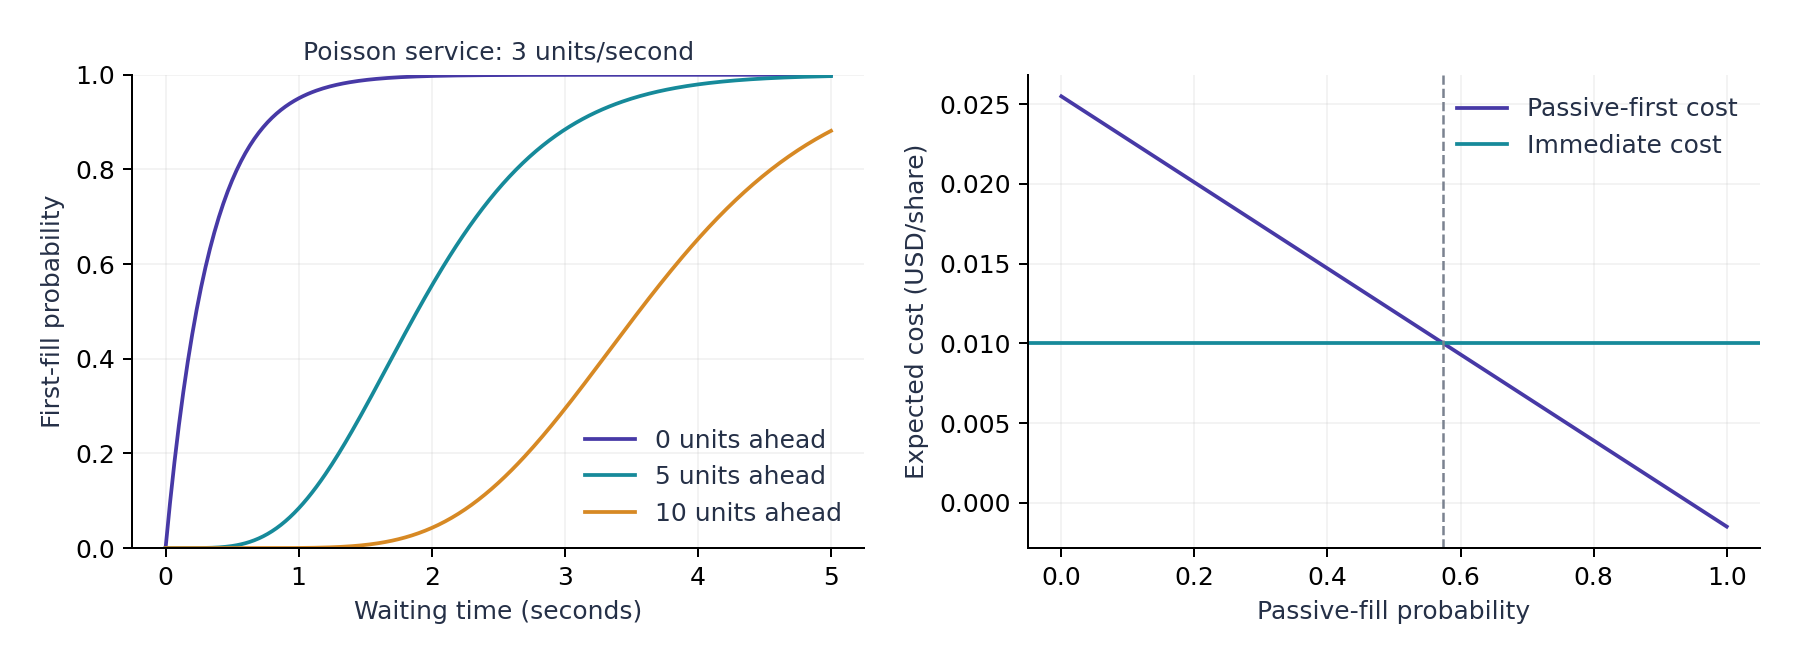
\includegraphics[width=\textwidth]{figures/03_queue_and_order_choice.png}
\caption{Two synthetic components of order choice. Left: first-fill probability
in the Poisson FIFO service model, with no cancellations or repricing. Right:
the passive-first cost threshold in Proposition~\ref{prop:threshold}.}
\label{fig:threshold}
\end{figure}

\section{Information value, misspecification and robust decisions}\label{sec:robust}

\subsection{Value of observing a liquidity signal}

In a finite-horizon model with hidden initial state $h$, fix a contingent policy
$\pi$ mapping future observations into actions. Its expected total cost at
prior $b$ is linear:
\begin{equation}\label{eq:policylinear}
 J_\pi(b)=\sum_hb(h)g_\pi(h),
\end{equation}
where $g_\pi(h)$ includes all later uncertainty and costs under that fixed
contingent plan. Suppose the feasible policy class is the same for every
prior in the comparison. Then $V(b)=\inf_\pi J_\pi(b)$ is concave.

\begin{proposition}[Free information cannot increase optimal expected cost]
Let $B$ be the posterior after an additional signal observed before choosing
the contingent plan. If $\E[B]=b$ and the signal does not change the underlying
feasible set or impose a cost, then
\begin{equation}\label{eq:voi}
 \E[V(B)]\leq V(b).
\end{equation}
\end{proposition}
\begin{proof}
An infimum of linear functions is concave. Jensen's inequality gives
$\E[V(B)]\leq V(\E B)=V(b)$. Equivalently, the informed trader can ignore the
signal and implement the prior-optimal plan.
\end{proof}

The result compares correct probabilistic information with the option not to
use it. It says nothing about the value of a misspecified hidden-stock feature,
a signal that arrives too late, or an information-gathering action with cost.
For a signal costing $c$, acquire it only when
$V(b)-\E V(B)>c$. The quantity on the left is specific to the decision loss;
it is not a price-prediction score.

\subsection{A finite-horizon decision bound}

\begin{theorem}[Regret from a wrong liquidity belief]\label{thm:belief}
Assume the same feasible contingent policies for priors $b$ and $\widehat b$.
For every such policy, suppose its conditional expected total cost has range
at most $C$: $\sup_hg_\pi(h)-\inf_hg_\pi(h)\leq C$.
Let $\widehat\pi$ minimize cost at $\widehat b$ and $\pi^*$ minimize it at $b$.
With $\TV(b,\widehat b)=\tfrac12\sum_h|b(h)-\widehat b(h)|$,
\begin{equation}\label{eq:beliefbound}
 0\leq J_{\widehat\pi}(b)-V(b)\leq 2C\,\TV(b,\widehat b).
\end{equation}
\end{theorem}
\begin{proof}
For a function of range at most $C$, the expectation difference between the
two priors is at most $C\TV(b,\widehat b)$. Apply this to each fixed policy
and add and subtract costs under $\widehat b$:
\begin{align*}
 J_{\widehat\pi}(b)-J_{\pi^*}(b)
 &= [J_{\widehat\pi}(b)-J_{\widehat\pi}(\widehat b)]
   +[J_{\widehat\pi}(\widehat b)-J_{\pi^*}(\widehat b)]\\
 &\quad+[J_{\pi^*}(\widehat b)-J_{\pi^*}(b)].
\end{align*}
The middle term is nonpositive by optimality. Bound the other terms as stated.
\end{proof}

An $\varepsilon$-optimal optimizer at $\widehat b$ adds $\varepsilon$ to the
right-hand side. If each of $N$ stage costs has range at most $c$ and terminal
cost range at most $c_T$, one may take $C=Nc+c_T$. Infinite hard-completion
penalties violate boundedness; this theorem then gives no finite guarantee.
The bound isolates belief error under an otherwise correct model. Wrong
transition kernels, impact laws or feasible sets require additional bounds.

\subsection{Robust control and tail objectives}

Let $\mathfrak K_k(X,a)$ be a set of plausible joint kernels. A robust recursion
is
\begin{equation}\label{eq:robust}
 V_k^{\rm rob}(X)=\min_{a\in\A_k(X)}\sup_{K\in\mathfrak K_k(X,a)}
                \E_K[c_k+V_{k+1}^{\rm rob}(X')].
\end{equation}
This stagewise form assumes rectangular uncertainty: nature can choose a
permitted kernel at each encountered state/action. If one unknown parameter
is fixed across the entire trajectory, independently maximizing at each step
changes the uncertainty model. A posterior over a fixed parameter or an
augmented robust state is then needed.

For a completed-order loss $L$, a tail criterion can use the representation
of \citet{rockafellar2000},
\begin{equation}\label{eq:cvar}
 \CVaR_\alpha(L)=\min_{z\in\R}
       \left[z+\frac{1}{1-\alpha}\E(L-z)_+\right],\quad 0<\alpha<1.
\end{equation}
Optimizing terminal CVaR is a precommitment problem unless the state and
criterion are adapted appropriately. Nesting one-step conditional risk
functionals gives a dynamically consistent alternative with a different
meaning. Neither CVaR nor a large inventory penalty makes a physically
impossible completion constraint feasible.

\section{NYSE and Nasdaq auctions at the deadline}\label{sec:auctions}

An auction is a distinct matching process with a clearing price and allocation
rule. It should not be modeled as a generic Poisson print near the open or
close. NYSE and Nasdaq publish distinct auction procedures and imbalance
information \citep{nyseauctions,nasdaqcross}. Reopening auctions depend on trading status and
event-specific rules. An imbalance observation is available only after its
dissemination time, even when the eventual auction price is known in a dataset.

\subsection{Exchange phases and commitment deadlines}

NYSE's opening process starts at 9:30 a.m. Eastern, but a DMM may open an
individual security later. Its published auction eligibility covers NYSE-listed
securities. Nasdaq describes broader cross eligibility, including nationally
listed securities \citep{nyseauctions,nasdaqcross}. The optimizer must retain
both the execution destination and the listing market. For a mandate tied to a
primary-market closing benchmark, a cross on another exchange must be evaluated
against that benchmark rather than assumed to reproduce it.

\begin{table}[tb]
\centering\small
\caption{Selected closing-auction constraints on a normal 4:00 p.m. close.
Times are Eastern; shortened sessions and exceptional events require their own
calendar and rules. Sources: \citet{nyseauctions,nysecloserule,nasdaqrules}.}
\label{tab:closedeadlines}
\begin{tabularx}{\textwidth}{p{.18\textwidth}YY}
\toprule Decision & NYSE & Nasdaq \\\midrule
Ordinary new MOC & Entry cutoff at 3:50; later entry has significant-imbalance conditions & Enter before 3:55 \\
Late LOC & After 3:50, significant-imbalance conditions apply & Before 3:58, with reference-price controls after 3:55 \\
Ordinary cancellation & MOC/LOC and Closing IO cancellations rejected from 3:50 & MOC/LOC ordinary cancellation ends at 3:50; specified error corrections only before 3:58 \\
Specialized late access & Established entry/cancel/modify cutoff: 3:59:50; amended cancel/modify cutoff: 3:59, subject to implementation & Imbalance-Only orders follow separate cross rules \\
\bottomrule
\end{tabularx}
\end{table}

The D Order row distinguishes the established process from the amendment
in SR-NYSE-2026-36. NYSE's published auction timeline states 3:59:50 for entry
and modification. The August 2026 filing changes cancellation/modification to
one minute before the close, but separately provides for implementation by a
Trader Update, anticipated no later than the first quarter of 2027. Its filing
effectiveness alone does not establish a production start date. Use the
announced implementation date to switch the constraint; do not apply 3:59
retroactively \citep{nyseauctions,nyse2026implementation}.

These times define changes in feasible actions, not just higher predicted
volume. At an irreversible commitment point, the relevant decision is whether
the prospective auction allocation is worth giving up the ability to redirect
those shares. A receding-horizon algorithm must optimize across the next such
boundary; waiting until the final minute can remove an entire order family
from its feasible set. Imbalance messages affect beliefs only after receipt,
and their indicative prices remain uncertain forecasts of clearing outcomes.

\subsection{Eligible interest, matched volume and the clearing problem}
\label{sec:auctionmath}

Fix an exchange $v\in\{\mathrm{XNYS},\mathrm{XNAS}\}$, auction $c\in\{o,k\}$
(opening or closing), and a realized pre-auction state $\omega$. All quantities
in this subsection are shares. Split each accepted order into accounting
pieces only when the pieces have different allocation classes; displayed and
reserve pieces must sum to the order's remaining quantity. For a candidate
price $p$, let $n_i(p;\omega)$ be the eligible quantity of piece $i$ after limit,
pegging, phase, access and other exchange restrictions have been applied.
For an ordinary buy limit $L_i$, eligibility requires $p\leq L_i$; for a sell,
$p\geq L_i$. Define executable demand and supply
\begin{equation}\label{eq:auctioncurves}
 D_v(p)=\sum_{i\in\mathcal B_v}n_i(p),\qquad
 S_v(p)=\sum_{j\in\mathcal S_v}n_j(p).
\end{equation}
The letter $S_v(p)$ here denotes a supply curve, not the reference-price process.
If every eligible buy can match every eligible sell, the maximum paired volume is
\begin{equation}\label{eq:auctionmin}
 V_v(p)=\min\{D_v(p),S_v(p)\},\qquad
 U_v(p)=D_v(p)-S_v(p).
\end{equation}
Paired volume counts each matched share once, not once on each side. The signed
quantity $U_v$ is an aggregate excess-demand statistic; it is not automatically
the exchange's published imbalance field.

When the remaining restrictions consist only of pairwise eligibility and
share capacities, the exact accounting object is a bipartite matching problem. Write $z_{ij}$ for the shares paired from buy
$i$ to sell $j$, and let $e_{ij}(p)\in\{0,1\}$ describe permitted matching:
\begin{align}\label{eq:auctionflow}
 V_v(p)&=\max_{z\geq0}\sum_{i,j}z_{ij},\\
 \sum_jz_{ij}&\leq n_i(p),\quad
 \sum_iz_{ij}\leq n_j(p),\quad
 z_{ij}=0\ \text{if }e_{ij}(p)=0.\nonumber
\end{align}
This formulation prevents an imbalance-offset instruction from being counted
as unrestricted two-sided liquidity. Additional priority constraints select
individual fills after price selection. Integer share capacities give an integer
maximum flow in this restricted bipartite problem. Minimum-fill conditions,
all-or-none requirements, state-changing self-trade prevention and other
non-pairwise constraints require additional integer or sequential rules; they
are not encoded by a fixed eligibility edge alone. With all pairings permitted,
\eqref{eq:auctionmin} follows: no flow can exceed either side's total, and a
successive pairing of eligible shares attains the smaller total.

The model therefore separates three maps: accepted orders to eligible interest,
eligible interest to an auction price, and the price plus allocation state to
individual fills. A generative auction model must preserve all three.

\subsection{Nasdaq: a lexicographic price-selection operator}

For Nasdaq's ordinary opening and closing crosses, Rules 4752(d) and 4754(b)
first maximize executed shares, then use unmatched on-open/on-close interest,
entered-price and midpoint tie-breaks; price protections and specified special
cases also apply \citep{nasdaqrules}. Let $\Pi$ be the applicable price grid and
write $I_c^N(p)$ for the rule-defined unmatched committed interest. In the
closing cross this statistic concerns MOC/LOC interest; in the opening cross
it also reflects the specified Early Market Hours interest. It need not equal
$|U_v(p)|$ when order classes differ.

A mathematical representation of the ordinary selection sequence is
\begin{align}\label{eq:nasdaqlex}
 \Pi_1&=\arg\max_{p\in\Pi}V_N(p),\\
 \Pi_2&=\arg\min_{p\in\Pi_1}I_c^N(p),\nonumber\\
 \Pi_3&=\begin{cases}E_c(\Pi_2),&E_c(\Pi_2)\ne\varnothing,\\\Pi_2,&E_c(\Pi_2)=\varnothing,\end{cases}\nonumber\\
 p_N^0&\in\arg\min_{p\in\Pi_3}|p-m_N|.\nonumber
\end{align}
To define $E_c$, fix a candidate price $p$ and provisionally allocate the
maximum paired volume under the cross's prescribed priority and compatibility
rules. Let $f_i^c(p)$ be that provisional fill of a priced, cross-eligible
piece $i$, $a_i^c$ its admitted quantity, and $e_i^c$ its entered price for
the ordinary cross, with any prescribed price treatment applied. In the
ordinary case the entered-price candidates are
\begin{equation}\label{eq:enteredset}
 E_c(A)=\left\{p\in A:
   \sum_{i:e_i^c=p}\bigl(a_i^c-f_i^c(p)\bigr)>0\right\}.
\end{equation}
Market interest without an entered price does not itself supply an entered-price
candidate. Provisional allocations are computed at each candidate; they do not
assume a previously selected auction price. The definition retains only prices
of residual priced interest when such candidates exist; otherwise the criterion
does not distinguish the surviving prices. Repricing and special ranked-price
adjustments must use the native rule's price fields and branches. In the
unrestricted subset, the provisional fills are given by
\eqref{eq:auctionfifo}; restricted matches require the compatibility rules too.
Here $m_N$ is the specified Nasdaq/system midpoint, not an arbitrary last trade.

For an example reaching this stage, let one buy LOC contain 600 shares at
\$100.02 and one sell LOC contain 500 shares at \$100.00. At the candidate
prices \$100.00, \$100.01 and \$100.02, paired volume is 500 and unmatched
LOC interest is 100. Only at \$100.02 does residual interest have an entered
price equal to the candidate, so $E_k(\Pi_2)=\{100.02\}$. The entered-price
criterion selects \$100.02 even if the system midpoint is \$100.01.
This example assumes an ordinary unrestricted cross and inactive price protections.
 Quantities and price conditions
are recomputed on the protected candidate set if the initially selected price
fails the applicable threshold condition. Opening validation and special
ranked-price adjustments remain explicit branches of the operator. A failed
opening validation may produce no opening cross; it is not repaired by a
fictitious execution at the nearest price.

Within the ordinary sequence, a later criterion cannot sacrifice a share
selected by an earlier criterion. The entered-price stage must be retained:
a weighted expression containing only volume, unmatched interest and midpoint
distance omits a rule even if its weights are small. A scalar encoding of all
stages would require bounds and minimum criterion gaps that rigorously preserve
the hierarchy. The subsequent protection and special ranked-price branches are
separate operations and may change the price selected by the ordinary sequence.

For forecasting, the current reference price and near/far indicative clearing
prices are different observables. The near calculation brings in eligible
continuous-book interest; the far calculation uses the corresponding auction
book \citep{nasdaqcrossfaq}. Neither is an already realized future auction price.
When market messages arrive, update the distribution of the complete future
input to \eqref{eq:nasdaqlex}, not merely a regression on one indicative number.

\subsection{NYSE: feasible prices and DMM auction liquidity}

NYSE Rules 7.35, 7.35A and 7.35B require a different construction. The DMM selects
the auction price; better-priced customer interest and auction-specific
conditions constrain that selection. Ordinary DMM Orders are not eligible for the closing auction under Rule
7.35B(a); DMM Auction Liquidity is a separate contribution that can be entered
after Core Trading Hours. DMM Auction Liquidity is excluded from
published Auction Imbalance Information, and DMM interest is not treated as
better-priced customer interest \citep{nyseauctiongeneral,nyseopenrule,nysecloserule}.
Consequently, a public maximum-volume calculation alone does not determine the
actual NYSE auction outcome.

Let $B_>(p)$ and $A_<(p)$ be eligible better-priced customer buy and sell
quantities, with the rule's treatment of market orders and short-sale
restrictions. Let $D_C(p),S_C(p)$ include eligible at-priced customer interest,
and let $L_D^b(p),L_D^s(p)$ denote DMM liquidity supplied for the auction.
Necessary aggregate feasibility conditions for full satisfaction of
better-priced customer interest are
\begin{equation}\label{eq:nysebetter}
 B_>(p)\leq S_C(p)+L_D^s(p),\qquad
 A_<(p)\leq D_C(p)+L_D^b(p).
\end{equation}
With restricted matches, these inequalities are replaced by the corresponding
flow-feasibility conditions from \eqref{eq:auctionflow}. They are necessary
accounting constraints, not a claim that a DMM is obliged to supply an unlimited
quantity at any proposed price.

For the ordinary closing case with a non-zero published Continuous Book Clearing
Price $p_{\rm CBC}$ and Imbalance Reference Price $r_k$, define
\begin{equation}\label{eq:nyseinterval}
\begin{split}
 \Pi_Y^k(\omega,L_D)=\bigl\{p\in\Pi:\;&
 \min(r_k,p_{\rm CBC})\leq p\leq\max(r_k,p_{\rm CBC}),\\
 &\text{\eqref{eq:nysebetter} and applicable conditions hold}\bigr\}.
\end{split}
\end{equation}
The interval comes from Rule 7.35B(g); the listed-ETP NAV exception and temporary
relief require separate states. The Continuous Book Clearing Price is itself a
rule-defined price for satisfying better-priced imbalance interest, not a
synonym for the price maximizing $\min(D_C,S_C)$ \citep{nyseauctiongeneral,nysecloserule}.

For an opening, use a separate set $\Pi_Y^o$ built from the opening reference,
applicable indications, timing, price conditions and \eqref{eq:nysebetter}.
The closing interval in \eqref{eq:nyseinterval} must not be copied into the
opening model. Opening time is a security-specific random time $\tau_o$, subject
to the DMM process, rather than a deterministic fill at exactly 9:30 a.m.
\citep{nyseopenrule}.

A forecasting model can now specify a conditional kernel
\begin{equation}\label{eq:dmmkernel}
 (p_Y,L_D,\tau_Y)\sim\mathcal H_{Y,c}
   (\cdot\mid\mathcal I_t,a),\qquad
 p_Y\in\Pi_Y^c(\omega,L_D),
\end{equation}
where $a$ includes the trader's proposed auction instruction. The DMM decision
is an uncertain external response for the execution optimizer. It is not a
control the customer can set. One may estimate $\mathcal H_{Y,c}$, integrate
scenario bounds, or explicitly condition on a stipulated DMM contribution in
an illustration. None of these choices licenses calling the DMM's unobserved
contribution measured hidden investor inventory.

\subsection{Allocation: Nasdaq order ranks and NYSE participant parity}

Once an auction price is fixed, total paired volume does not determine a child's
fill. In a Nasdaq subset without restricted counterparties, sort eligible
pieces on a given side in the cross's prescribed order $i_1,\ldots,i_m$. The
ordinary hierarchy places market-on-auction interest first, followed by the
specified displayed class and then non-displayed interest, with the rule's
price/time priorities inside the classes \citep{nasdaqrules}. If $V$ shares on
that side can execute, the rank recursion is
\begin{equation}\label{eq:auctionfifo}
 R_0=V,\qquad F_{i_j}=\min\{n_{i_j},R_{j-1}\},\qquad
 R_j=R_{j-1}-F_{i_j}.
\end{equation}
The restriction on counterparties must still be respected; the recursion is
not a substitute for the eligibility edges in \eqref{eq:auctionflow}.

For NYSE, allocate eligible better-priced customer interest first, and let
$R$ be the residual capacity on one side. At-priced interest then passes through
auction-specific classes. The following is the ordinary hierarchy, with DMM
positioning and exceptional states supplied by the cited rules.

\begin{table}[tb]
\centering\small
\caption{NYSE residual allocation after better-priced customer interest.
Sources: \citet{nyseopenrule,nysecloserule}.}
\label{tab:nyseauctionpriority}
\begin{tabularx}{\textwidth}{p{.08\textwidth}YY}
\toprule Stage & Opening & Closing \\\midrule
1 & Displayed class, Opening D Orders and LOO: participant parity & Displayed class and Closing D Orders: participant parity \\
2 & Non-displayed class: participant parity & Non-displayed class: participant parity \\
3 & Displayed yielding interest: time & LOC: time \\
4 & Non-displayed yielding interest: time & Closing IO opposite the unpaired side: time \\
5--6 & --- & Displayed, then non-displayed yielding interest: time \\
\bottomrule
\end{tabularx}
\end{table}

Thus a NYSE LOC at the auction price does not receive the same treatment as a
NYSE LOO at the opening price. A Closing D Order is also not interchangeable
with an LOC submitted by the same intermediary. Continuous-market setter
priority does not carry into the closing auction \citep{nysefaq}.

Inside a NYSE parity class, the allocation wheel identifies the next eligible
participant. With round lot $\ell$, residual capacity $R$ and participant
capacity $n_j$, an ordinary wheel visit allocates
\begin{equation}\label{eq:auctionwheel}
 f=\min\{\ell,n_j,R\},\qquad n_j\leftarrow n_j-f,\quad R\leftarrow R-f,
\end{equation}
and advances according to Rule 7.37. Odd-lot handling and pointer retention
are additional branches. The Book Participant's allocation is then assigned
by working time; Floor Broker allocation has its own internal parity process
\citep{nyseallocationrule}. An upstairs order is part of the Book Participant,
not automatically a separate slot in the wheel.

In a divisible-share approximation, after higher classes are satisfied, equal
participant sharing with capacity constraints is summarized by
\begin{equation}\label{eq:fluidparity}
 F_j=\min\{n_j,\theta\},\qquad
 \sum_j\min\{n_j,\theta\}=\min\{R,\sum_jn_j\}.
\end{equation}
This is a fluid approximation to repeated visits, not NYSE's exact share and
pointer rule. For capacities $(600,300,300)$ and $R=600$, it gives
$(200,200,200)$, which also follows from two complete 100-share wheel rounds.
A global FIFO allocation with the 600-share interest first gives $(600,0,0)$.
The difference is economically material even though the price and total volume
are identical.

\subsection{A worked clearing example for the two exchanges}

Consider the following artificial closing book, in shares. The limit orders
are LOCs; there are no reserves, restricted pairs, short-sale restrictions,
yielding instructions or binding price protections. This is a small mechanism
example, not a calibration or a venue-performance comparison.
\begin{center}\small
\begin{tabular}{lrrr}
\toprule Side & Market-on-close & Limit 100.01 & Limit 100.02 \\\midrule
Buy & 300 & 400 & 500 \\
Sell & 200 & 600 & 300 \\
\bottomrule
\end{tabular}
\end{center}
The resulting executable curves are
\begin{center}\small
\begin{tabular}{rrrrr}
\toprule Price & Demand & Supply & Paired volume & Demand minus supply \\\midrule
100.00 & 1200 & 200 & 200 & 1000 \\
100.01 & 1200 & 800 & 800 & 400 \\
100.02 & 800 & 1100 & 800 & $-300$ \\
100.03 & 300 & 1100 & 300 & $-800$ \\
\bottomrule
\end{tabular}
\end{center}

For the Nasdaq example, $\$100.01$ and $\$100.02$ tie on maximum volume at
800 shares. Because all interest is MOC/LOC and unrestricted, the tie-break
compares the unmatched imbalance at the two tied prices: 400 shares of
excess demand at $\$100.01$ against 300 shares of excess supply at
$\$100.02$. The smaller imbalance selects $\$100.02$ and 800 matched shares.
Buy fills are
300 MOC plus 500 LOC; sell fills are 200 MOC plus 600 LOC at the more aggressive
limit. The remaining 300-share sell LOC is unfilled.

For the NYSE example, stipulate a last-published reference price of \$100.00
and Continuous Book Clearing Price of \$100.01. The latter is consistent with
this book: at \$100.01 the 800 better-priced customer buy shares can be
satisfied by 800 eligible sell shares. With no DMM contribution, \$100.01 is a
feasible selected price with 800 matched shares. If the DMM instead supplies
200 eligible sell shares at that price, 1000 shares can match and 200 of the
400-share at-priced buy LOC can execute. DMM participation and price selection
are stated assumptions of this NYSE scenario, not quantities inferred from the
public imbalance. The Nasdaq maximum-volume tie-break cannot be used to rule
out the stipulated NYSE price.

\subsection{Auction impact and the optimal committed quantity}

A useful local approximation explains why auction liquidity changes the
schedule. Suppose all submitted auction shares fill, and a smooth competitive
clearing equation is
\begin{equation}\label{eq:auctionlocal}
 D_0(p)+y=S_0(p),\qquad S_0'(p)-D_0'(p)>0,
\end{equation}
where $y$ is the trader's buy quantity. Implicit differentiation gives
\begin{equation}\label{eq:auctionimpact}
 \frac{\partial p}{\partial y}
 =\frac{1}{S_0'(p)-D_0'(p)}.
\end{equation}
With price measured in dollars per share, the denominator has units shares
squared per dollar, and $\partial p/\partial y$ has units dollars per share
squared. Deeper marginal auction supply reduces price sensitivity. This is a
smooth local model: real price grids, tie-breaks, allocation changes and a DMM's
discrete response can make $p(y)$ discontinuous. For a smooth NYSE scenario in which DMM response depends only on price,
replace the denominator by $S_0'+\partial_pL_D^s-D_0'-\partial_pL_D^b$.
If it also depends directly on the submitted quantity, the derivative is
\[
 \frac{\partial p}{\partial y}=
 \frac{1+\partial_yL_D^b-\partial_yL_D^s}
 {S_0'+\partial_pL_D^s-D_0'-\partial_pL_D^b},
\]
provided the denominator is nonzero. These response derivatives are model
assumptions to estimate or stress, not exchange rules.

For a fully filled buy commitment, dollar execution cost relative to $s$ is
$C_A(y)=y[p(y)-s+f_A]$. Its marginal cost is
\begin{equation}\label{eq:auctionmarginalimpact}
 C_A'(y)=p(y)-s+f_A+y\,p'(y).
\end{equation}
The last term matters: increasing the commitment can change the price of every
share in the auction order. Treating the indicative price as an exogenous
quote drops that effect.

\begin{proposition}[A schedule with an auction endpoint]\label{prop:auctionendpoint}
Suppose $Q-y$ shares are completed continuously and $y$ are filled in a final
auction. Let their modeled costs be
$C_C(x)=a_Cx^2+c_Cx$ and $C_A(y)=a_Ay^2+c_Ay$, with an additional exposure
penalty $r_Ay^2$, where $a_C,a_A,r_A\geq0$ and their sum is positive. Then
\begin{equation}\label{eq:auctionquantity}
 y^*=\clip_{[0,Q]}
 \left(\frac{2a_CQ+c_C-c_A}{2(a_C+a_A+r_A)}\right).
\end{equation}
\end{proposition}
\begin{proof}
The objective is $J(y)=C_C(Q-y)+C_A(y)+r_Ay^2$. Its derivative is
$2(a_C+a_A+r_A)y-2a_CQ-c_C+c_A$ and its second derivative is strictly positive.
The constrained minimizer is the unconstrained root projected onto $[0,Q]$.
\end{proof}

For $Q=1000$, $a_C=2\times10^{-5}$, $a_A=r_A=10^{-5}$,
$c_C=0.012$ and $c_A=0.002$, the optimum is $y^*=625$ auction shares and
375 continuous shares. The synthetic objective is \$16.375, compared with
\$32 for continuous completion and \$22 for committing all shares to the auction.
These amounts combine execution costs and the chosen exposure penalty.
Figure~\ref{fig:auctionmath} and \texttt{scripts/auction\_examples.py} reproduce
the clearing curves, allocation contrast and endpoint calculation.

\begin{figure}[tb]
\centering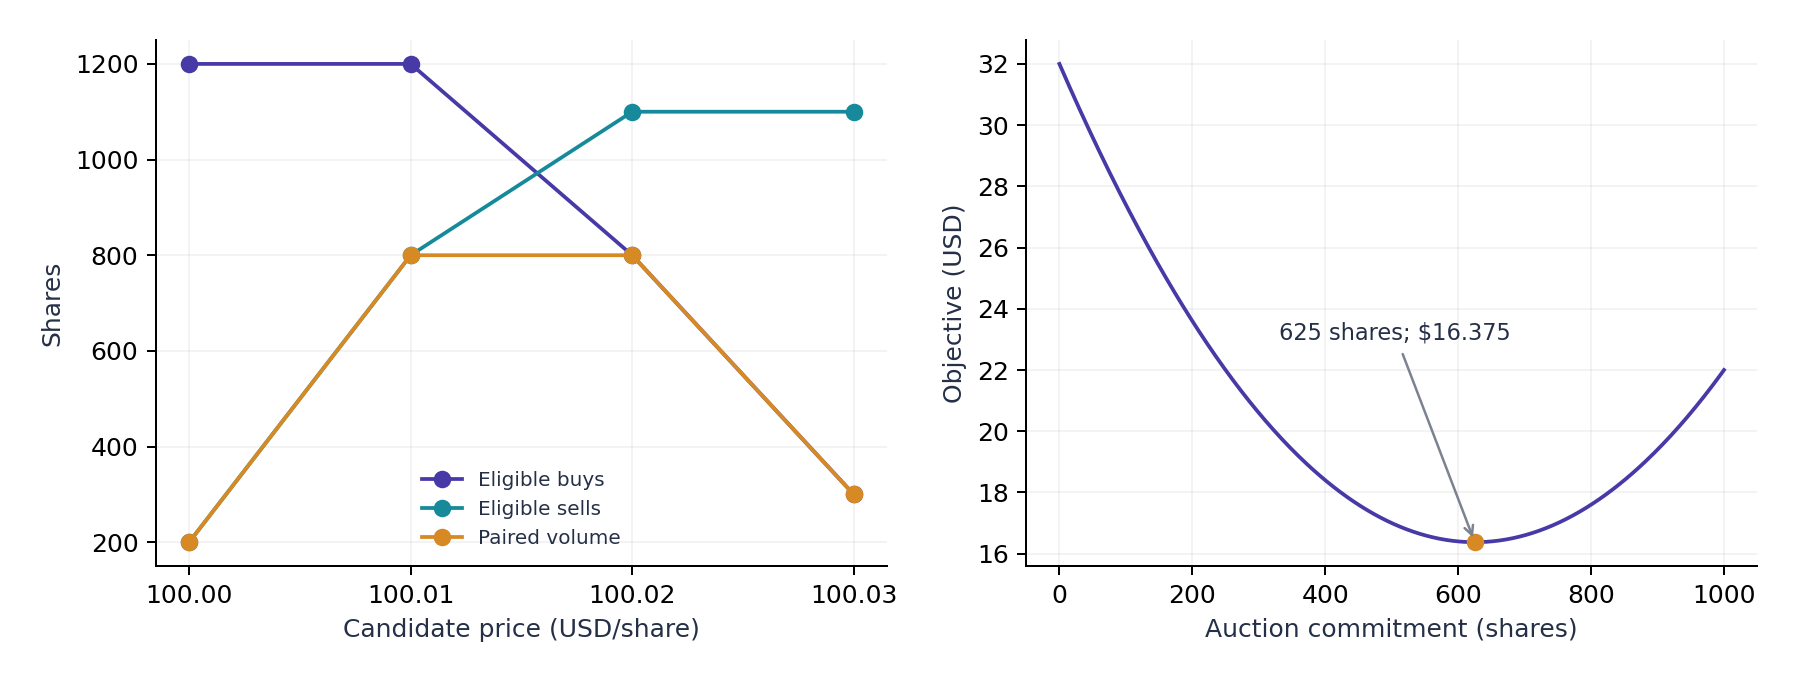
\includegraphics[width=\textwidth]{figures/07_auction_math.png}
\caption{Synthetic auction illustrations: the two candidate Nasdaq prices tie on
volume but differ in unmatched interest; the endpoint cost model has an interior
optimum at 625 auction shares. Parameters and assumptions are given in the text.}
\label{fig:auctionmath}
\end{figure}

Full auction fills are a restrictive assumption. With random fill $F(y)$,
price $P(y)$ and residual completion cost $\Phi$, a single-auction split becomes
\begin{equation}\label{eq:auctionpartialobjective}
 J(y)=C_C(Q-y)+\E\!\left[
 F(y)(P(y)-s+f_A)+\Phi(y-F(y))\right].
\end{equation}
Assume a common exogenous scenario variable with a distribution independent
of $y$, pathwise differentiable $F(y)$ and $P(y)$, and an integrable bound
justifying differentiation under expectation. Then its derivative is
\begin{align}\label{eq:auctionpartialderivative}
 J'(y)=-C_C'(Q-y)+\E\!\left[
 F'(y)(P(y)-s+f_A)+F(y)P'(y)\right.\qquad\\[-4pt]
 \left.{}+\Phi'(y-F(y))(1-F'(y))\right].\nonumber
\end{align}
This expression separates the value of an extra fill, the effect on clearing
price, and the cost of an extra unfilled share. In a discrete exchange model,
use finite differences of the full action-dependent expected objective instead of differentiating
through tick, priority or cutoff discontinuities. If the scenario distribution
itself varies with $y$, its derivative also contributes a distributional term;
a pathwise formula alone does not include that term.

For commitments to both modeled destinations, use their joint law, not
independent auction simulations:
\begin{equation}\label{eq:twoauctionobjective}
 \min_{x,y_N,y_Y}\ C_C(x)+
 \E\!\left[\sum_{v\in\{N,Y\}}F_v(y_v)(P_v-s+f_v)
       +\Phi\!\left(q-x-\sum_vF_v(y_v)\right)\right],
\end{equation}
subject to nonnegative quantities, exchange eligibility and
$x+y_N+y_Y\leq q$ after allowing for outstanding commitments. Shared news and
order flow couple the outcomes. Auction access may force one commitment to
zero; in particular, a non-NYSE-listed security is not eligible for the NYSE
primary auction. Deadline constraints and the actual residual opportunity set
must make the terminal term attainable. The following valuation discussion
applies this accounting to the mandate's benchmark.



\subsection{Valuing the auction allocation}

Let $y$ be quantity committed to an auction, $F^A\leq y$ its random allocation,
and $P^A$ its clearing price. An appropriate terminal opportunity has value
\begin{equation}\label{eq:auction}
 \E\left[F^A(P^A-S_0+f^A)
          +\Phi(q-F^A,S_T,r_T)\mid \mathcal I, y\right],
\end{equation}
where $\mathcal I$ includes only known imbalance, reference and phase data.
Price and allocation are generally dependent. A limit-on-close order can
bound an acceptable price while failing to execute. A market-on-close order
does not fix the clearing price.

For intuition only, suppose auction fill is deterministic, its incremental
cost is $ay^2+\mu_Ay$, and continuously executing the rest costs $G(Q-y)$.
An interior allocation solves
\begin{equation}\label{eq:auctionmarginal}
 2ay+\mu_A=G'(Q-y).
\end{equation}
This is another marginal-value condition, but deterministic fill is an
assumption of the example. With uncertain allocation, minimize
\eqref{eq:auction} using a joint distribution and a valid residual rule.

Auction commitments consume parent capacity until resolved. After a cutoff,
cancellation may be restricted, so the trader loses an option to reallocate
quantity. A state variable for cancellability is therefore necessary. If the
closing auction is the final admissible opportunity, a simulator cannot repair
a missed allocation by assuming an unlimited post-deadline market order.
One must reserve earlier completion capacity, accept a specified residual,
or change the mandate. Exact cutoffs are instrument-, event- and rule-dependent
inputs, not universal constants supplied by the optimization model.

\part{Numerical illustrations}\label{pt:experiments}
\section{Reproducible numerical illustrations}\label{sec:experiments}

The examples support the theoretical development by checking arithmetic and
showing which economic decisions the assumptions produce. Every parameter is
stipulated below and in the executable source. The examples are model
illustrations; no parameter was estimated from Nasdaq or NYSE records.

\subsection{Analytic schedule and immediate routing}

Set $Q=T=\eta=1$ in Proposition~\ref{prop:acsinh}. Define the unweighted impact
term $I=\int_0^1v_t^2\dd t$ and exposure $R=\int_0^1q_t^2\dd t$.
Table~\ref{tab:schedules} reports numerical quadrature on 2,001 equally spaced
points. Each row uses a different objective weight $\kappa^2$; its last
column should not be compared as if all rows solved the same objective.
At $\kappa=3$, the greater impact cost purchases a substantial reduction in
unweighted exposure.

\begin{table}[tb]
\centering
\caption{Normalized analytic schedule calculations.}
\label{tab:schedules}
\begin{tabular}{rrrr}
\toprule $\kappa$ & Impact $I$ & Exposure $R$ & $I+\kappa^2R$ \\\midrule
0 & 1.0000 & 0.3333 & 1.0000 \\
1 & 1.0185 & 0.2945 & 1.3130 \\
3 & 1.5523 & 0.1625 & 3.0149 \\

\bottomrule
\end{tabular}
\end{table}

For routing, set $C_v(x)=a_vx+b_vx^2/2$ with
\begin{equation}\label{eq:routeparams}
 a=(0.010,0.012,0.014),\quad
 b=(0.000080,0.000025,0.000012),\quad
 c=(120,550,900).
\end{equation}
Here quantities are shares, $a$ is dollars per share and $b$ is dollars per
share squared. The 1,000-share allocation in Table~\ref{tab:routing} costs
\$16.6106 in this model. Venue A has the lowest initial cost but reaches its
120-share cap. Venues B and C equalize marginal cost at about 2.04865 cents
per share; A's lower marginal cost at capacity is consistent with
\eqref{eq:kkt}. Decimal allocations solve a continuous relaxation. Integer
shares can be obtained by solving the corresponding discrete marginal-cost
allocation; the decimals are not submitted orders.

\begin{table}[tb]
\centering
\caption{Synthetic routing of 1,000 shares; continuous relaxation.}
\label{tab:routing}
\begin{tabular}{lrrr}
\toprule Venue & Shares & Cost (USD) & Marginal cost (cents/share) \\\midrule
A & 120.00 & 1.7760 & 1.9600 \\
B & 339.46 & 5.5139 & 2.0486 \\
C & 540.54 & 9.3207 & 2.0486 \\

\bottomrule
\end{tabular}
\end{table}

\subsection{A finite-horizon liquidity-learning problem}

The dynamic example buys $Q=20$ units, with one unit defined as 100 shares,
over $K=12$ waiting intervals followed by terminal completion. This unit is
a numerical scale, not an assertion about a security's effective round lot.
A hidden regime $H\in\{0,1\}$ is drawn once per trajectory and remains fixed.
Its initial probability is $\Pp(H=1)=1/2$. Prices carry no information about
$H$; only the controlled fill observations update its posterior.

At each step choose $m\in\{0,\ldots,q\}$ immediate units, a passive size
$\ell\in\{0,\min(1,q-m),\min(3,q-m),\min(5,q-m)\}$, and one of two
passive channels when $\ell>0$. Require $m+\ell\leq q$. All immediate units
fill at charge
\begin{equation}\label{eq:simmarket}
 C_M(m)=m+0.08m^2\quad\text{USD}.
\end{equation}
Passive fills satisfy
\begin{equation}\label{eq:simfill}
 F\mid H,v,\ell\sim\operatorname{Binomial}(\ell,p_{v,H}),\qquad
 (p_{v,H})=\begin{pmatrix}0.15&0.60\\0.05&0.75\end{pmatrix}.
\end{equation}
The rows are a stylized displayed passive channel and a midpoint channel;
the columns are the less and more liquid hidden regimes. The displayed
channel has net charge $-\$0.30$ per filled unit and the midpoint channel
$\$0.05$. These hypothetical net charges are not an actual fee schedule.
All passive orders expire before the next decision, so there are no live
orders across intervals in this example.

After the interval, $q'=q-m-F$ and the inventory penalty is
$0.008(q')^2$ dollars. At the terminal time all remaining units execute at
$C_M(q)$. The objective is
\begin{equation}\label{eq:simobjective}
 \E\left[\sum_{k=0}^{K-1}
   \{C_M(m_k)+c_{v_k}F_k+0.008q_{k+1}^2\}+C_M(q_K)\right].
\end{equation}
The penalty is a specified risk preference. Independent zero-mean reference
innovations can be integrated out of expected execution cost; they are not
sampled in the reported Monte Carlo calculation. Consequently, the reported
standard errors describe regime and fill randomness, not the distribution
of full realized dollar shortfall under a sampled price process.

The unit fills in \eqref{eq:simfill} are independent conditional on regime,
size and venue. Across intervals they are dependent through the persistent
regime. This abstraction omits queue position, impact resilience, price changes
conditional on fills, and venue-specific order protocols. It is chosen to
isolate the scheduling value of learning execution availability. The general
framework permits those omitted states; this small experiment does not validate
them.

\subsection{The six policies}

The \emph{belief policy} solves the Bellman recursion on 101 equally spaced
belief values. It updates the posterior from the exact binomial likelihood
after both fills and non-fills. Continuation values are linearly interpolated
in belief; simulation selects the action at the nearest belief grid point.
This is an approximate solution of the finite-action partially observed problem.

The \emph{frozen-prior} comparator is separately optimized under a model that
keeps the regime mixture fixed at its initial value at each future step. Its
Bellman recursion suppresses posterior updates. It therefore describes a
misspecified non-learning model of persistent liquidity, rather than simply
reusing the learning controller and withholding its state. It is evaluated
on the same persistent-regime trajectories as every other policy.

The \emph{regime oracle} observes $H$ before trading and uses the corresponding
endpoint-belief policy. It has more information but the same order-size and
venue choices. It is an information benchmark, not an available trading strategy.
\emph{TWAP market} divides residual inventory across remaining opportunities,
rounding the next quantity upward to integer units. \emph{Market now} buys all
20 units at the first decision. \emph{Midpoint first} posts up to five units
at the midpoint at each step and completes the remainder at the terminal time.

\subsection{Results and their interpretation}

All six policies use the same 16,000 regime draws and per-step uniform random
numbers. With NumPy generator seed 5257, the implementation draws the regime
uniforms first and then a path-major $16000\times12$ array of fill uniforms.
Binomial inverse distribution functions map those common uniforms to fills. Common random numbers support paired comparisons;
their role is variance reduction, not a source of independent market evidence.
Table~\ref{tab:policies} decomposes the objective into execution charges and
the inventory penalty.

\begin{table}[tb]
\centering\small
\caption{Synthetic policy comparison for a 2,000-share parent. Charges, penalties,
objectives and Monte Carlo standard errors are in USD. Terminal quantity is
the mean number of 100-share units before forced completion.}
\label{tab:policies}
\begin{tabular}{lrrrrr}
\toprule Policy & Charge & Penalty & Objective & MC SE & Terminal units \\\midrule
\inputtable{tables/policy_rows.tex}
\bottomrule
\end{tabular}
\end{table}

The belief policy has mean objective \$\BeliefObjective\ versus
\$\FrozenObjective\ for the optimized frozen-prior model, a reduction of
\ImprovementPct\%. The paired difference is \$\PairedDifference\ with
standard error \$\PairedSE; a normal Monte Carlo 95\% interval is
[\$\CILower,\$\CIUpper]. This interval describes numerical sampling under
the specified model, not parameter-estimation error or market uncertainty.

Execution charges alone are \$\BeliefCharge\ for the belief policy and
\$\FrozenCharge\ for the frozen-prior comparator. The improvement therefore
comes principally from reducing the inventory penalty, from
\$\FrozenPenalty\ to \$\BeliefPenalty, while reducing mean residual
quantity before terminal completion. The oracle's mean objective is
\$\OracleObjective; its advantage over the belief policy is \$\OracleGap\
with paired standard error \$\OracleGapSE. This is a cost of incomplete
regime information within the stipulated model.

Midpoint-first leaves substantial quantity for expensive terminal completion
in the less liquid regime. Market-now avoids the inventory penalty but pays
the largest quadratic immediate charge. Changing fill probabilities, impact
coefficients or risk preferences can change these rankings.

\begin{figure}[tb]
\centering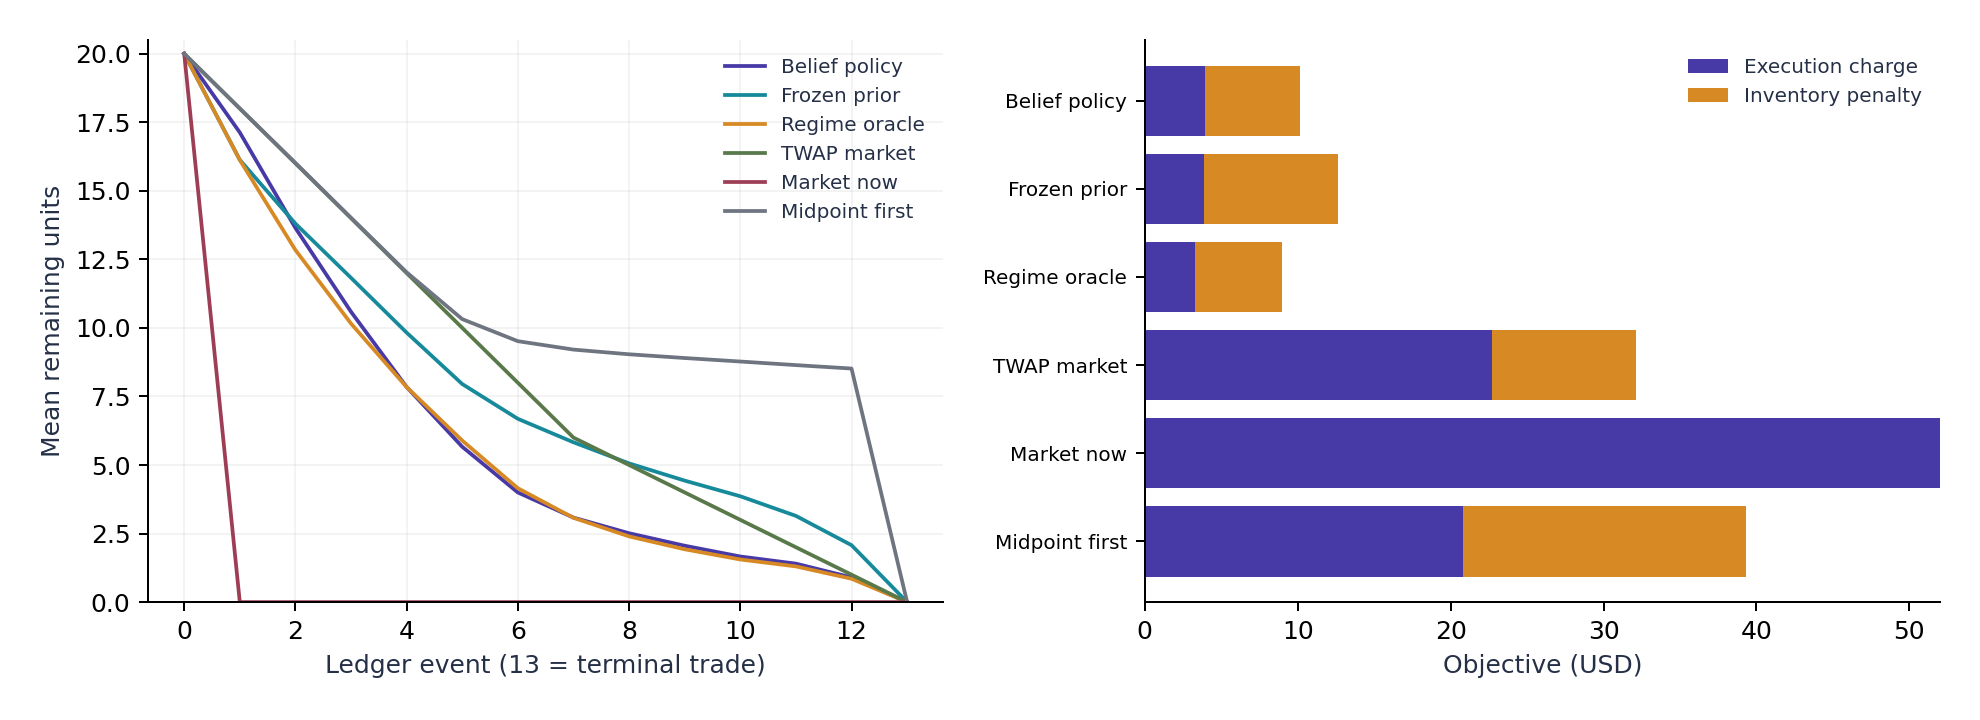
\includegraphics[width=\textwidth]{figures/05_policy_comparison.png}
\caption{Synthetic execution paths and objective decomposition. The left panel
plots mean residual quantity after successive ledger events; its final point
is the terminal completion trade, not an extra waiting interval. The right
panel separates execution charges from the chosen inventory penalty.}
\label{fig:policies}
\end{figure}

\begin{figure}[tb]
\centering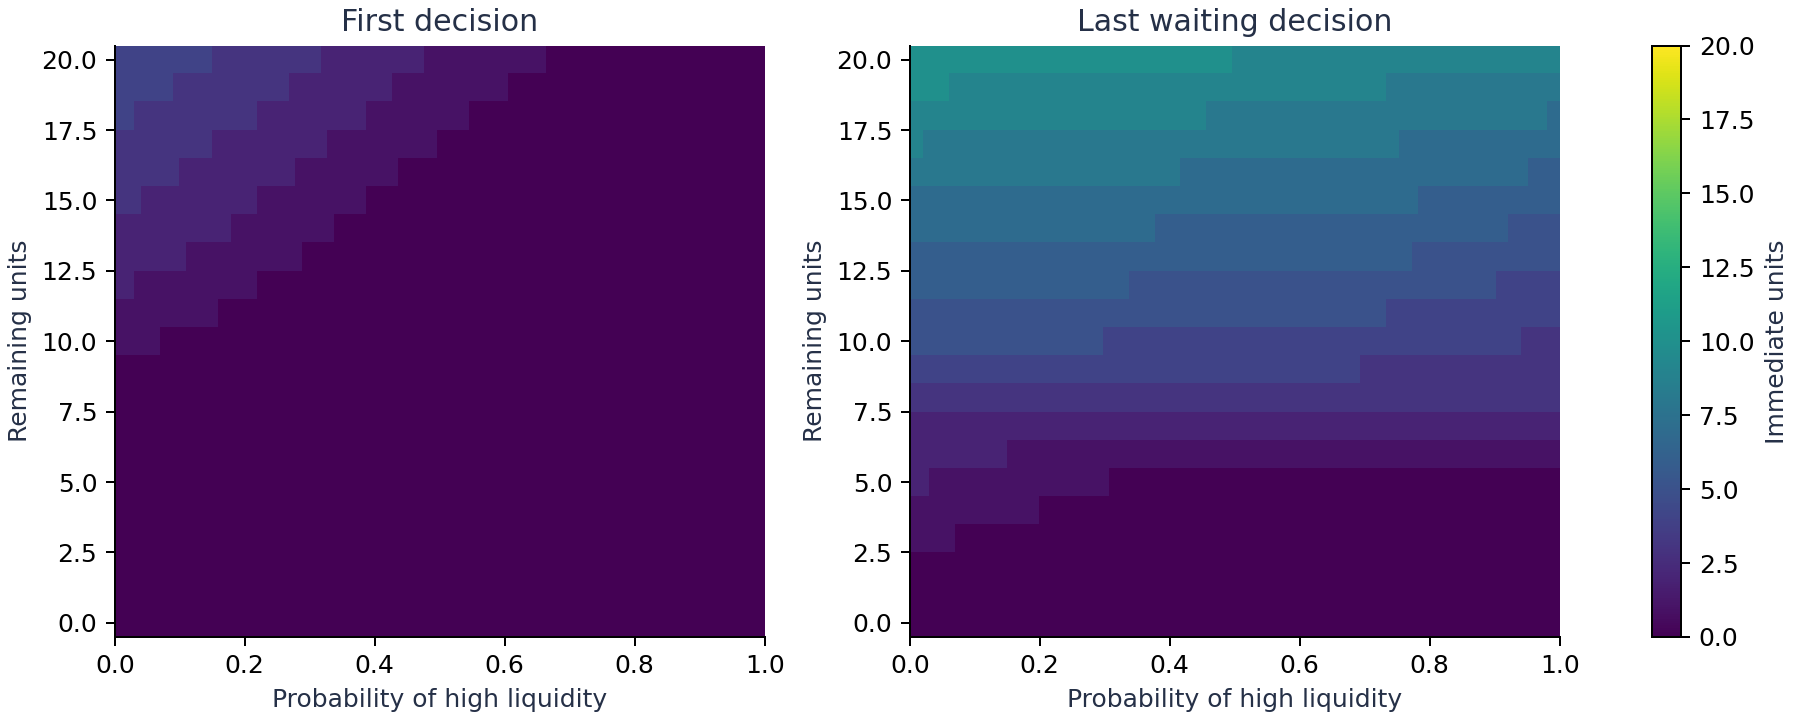
\includegraphics[width=\textwidth]{figures/06_urgency_and_belief.png}
\caption{Immediate quantities selected by the approximate belief policy at the
first and last decisions, over remaining inventory and belief. The state
includes both urgency and execution availability. Color scales are shared.}
\label{fig:heatmaps}
\end{figure}

Every simulated parent completes, because unlimited terminal market execution
is a declared assumption. The simulation also enforces $m+\ell\leq q$.
These checks establish quantity consistency in the toy model; they do not
establish that a live exchange would provide terminal liquidity or that
asynchronous cancellation is safe. Proposition~\ref{prop:reserve} addresses
the separate accounting condition for live orders.

\subsection{Numerical checks and limits}

The interpolated initial value is \$\InitialValue. Increasing the belief grid
from 101 to 201 points changes that value by \$\GridError. This is a targeted
resolution check at the stated initial condition, not a uniform policy-error
bound. The simulated mean differs from the coarser grid value by $\$0.0402$,
i.e.\ $0.51$ of the belief policy's reported Monte Carlo standard error of
$\$0.078$ (Table~\ref{tab:policies}); nearest-grid action selection and
simulation are separate from interpolation in the Bellman recursion.

The source also checks the pathwise shortfall identity on 500 independently
generated completed ledgers, the posterior-mean identity for binomial
observations, the immediate-allocation quantity constraint, and the reserve
transfer example. All figures and numerical tables are generated from the same
Python script and JSON results. Code and parameter files permit the reader to
change probabilities, capacities, impact, horizon or risk preference without
substituting undocumented assumptions.

The tests deliberately do not claim superiority of LSTMs, transformers or
reinforcement learning. A small partially observed example can be solved by
dynamic programming and provides a useful benchmark for more flexible methods.
Market-calibrated conclusions require the additional evidence described next.

\subsection{Testing the exact-completion certificate}\label{sec:certexperiment}
The additional experiment tests \cref{thm:completion,thm:certificate} directly.
Set $X=T=1$, $\bar V=2$, $\eta=0.15$, and let $U$ be uniform on
$\{0,0.2,0.4,0.6,0.8,1\}$. The exogenous path is
$Y_t=(t,(t-U)_+)$, the true kernel is $e^{-t}$, and an observed linear
execution charge is $a_t=-0.3(t-U)_+$. Use the features
$\phi=(1,t,(t-U)_+)$ in \eqref{eq:completionfeatures} with
$M=(1,1/2,1/2)$ and coefficient budget $r=1$. Thus every tested policy
completes exactly and stays in $[0,2]$ for all $U\in[0,1]$, not just at
the sampled support points. An Euclidean coefficient bound is $R=2$.

For each approximate decay rate in $\{0.9,1,1.1\}$, fit the objective using
a multinomial sample of $100$, $1000$ or $10000$ exogenous paths, with a
separate fixed seed 525717. State-ODE integration computes the quadratic and
linear coefficients independently of the signature shuffle implementation.
The true finite law supplies the matrix and linear coefficient errors; the
kernel error is bounded in the uniform norm and the optimizer reports its
convex duality gap. Table~\ref{tab:certificate} compares actual regret within
this coefficient polytope with \eqref{eq:certificate}.

\begin{table}[tb]
\centering\small
\caption{Synthetic verification of the execution certificate. Errors are
measured against the known finite law; the bounds are deterministic for these
realized estimates, not statistical confidence intervals.}
\label{tab:certificate}
\begin{tabular}{rrrr}
\toprule Decay rate & Paths & Actual class regret & Certificate \\\midrule
\inputtable{tables/certificate_rows.tex}
\bottomrule
\end{tabular}
\end{table}

All nine cases satisfy the bound. The certificate can be conservative because
it is uniform over the coefficient class and combines worst-case matrix and
linear errors. Larger samples need not improve every realized estimate
monotonically. No claim about an unknown market distribution follows from
measuring errors against this known synthetic law.

\begin{figure}[tb]
\centering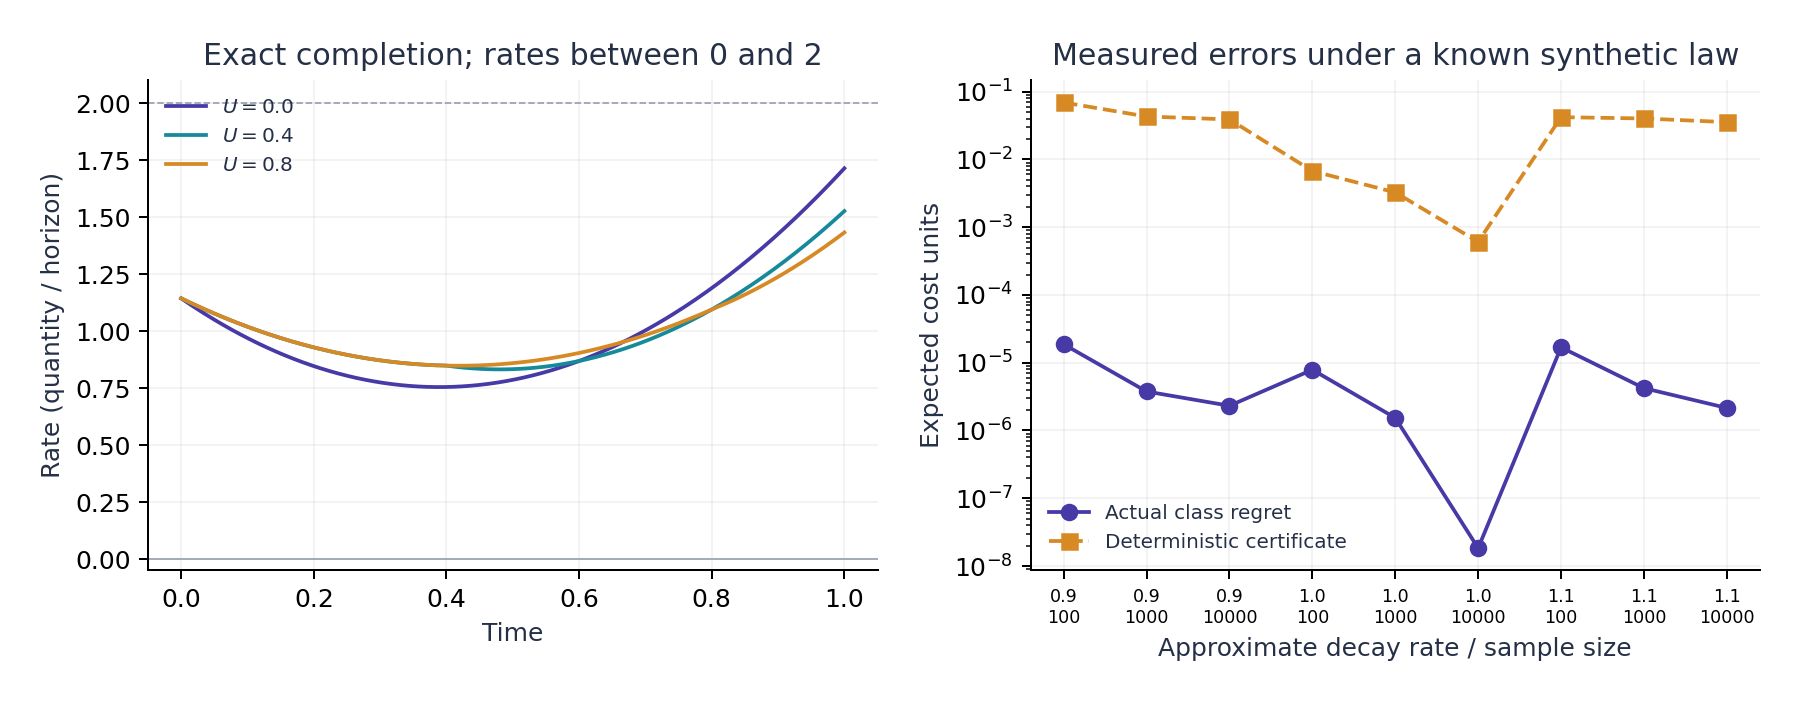
\includegraphics[width=\textwidth]{figures/08_execution_certificate.png}
\caption{Left: feasible rates from the true-law optimum for three signal paths.
Right: actual class regret and its deterministic certificate in the nine
kernel-and-sampling scenarios. Exact completion follows analytically from the
feature construction; the numerical checks also integrate every rate.}
\label{fig:certificate}
\end{figure}

The algebra is checked separately on six kinked paths with a depth-one rate
using time, the signal and both exponential coordinates. Integrating the
required signature coordinates and an independent impact-state ODE gives
costs agreeing within $10^{-10}$. This verifies the numerical implementation
of the exact finite-degree identity; the proof remains
\cref{thm:sigquadratic}. Further checks reproduce the finite-signature
counterexample, the cutoff correction, the sharp binary information constant,
and the cell-averaged Riesz energy.

\subsection{A tagged book, a learned controller and a rate certificate}\label{sec:bookexperiment}

The final illustration implements the construction in \cref{sec:bookbridge}.
A parent buys one share on a synthetic two-price book with bid $100$ and ask
$101$. Up to two external bid units and one own unit can rest at the bid;
one external ask unit can rest at the ask. External bid arrivals, ask
arrivals and unit buys have rates $0.4$, $0.6$ and $0.5$ per second. Each
existing external bid cancels at rate $0.15$. Unit sells arrive at true rate
$\lambda=1.2$. Buy and sell requests are immediate-or-cancel against the
opposite quote. At capacity an external limit arrival is rejected; if an
opposite queue is empty an immediate-or-cancel request expires. All matching
uses the actual ordered queues, with executions at resting prices.

The nine possible bid queues are three unposted queues with zero, one or two
external units, and six queues with one own unit inserted at every possible
position among them. Combined with two ask occupancies and a stopped state
after parent completion, this gives 19 states. The initial book has two
external bid units and one ask unit, with no own order. There are four
decisions at $0,0.25,0.5,0.75$ seconds and a deadline at $T=1$. An action
posts or retains the own bid, cancels it and waits, or cancels it and crosses
an available ask. Cancellation is atomic in this example. A retained order
keeps its priority. A separately stipulated terminal facility buys any
remaining unit at $102$, so completion is guaranteed even when the local
ask is empty. This facility is an explicit model assumption, not inferred
liquidity in the book.

Costs are measured relative to $100$: a passive fill costs $0$, an aggressive
fill costs $1$, and terminal completion costs $2$. No additional message,
risk or impact charge is imposed. Consequently every complete path loss
lies in $[0,2]$. Posting is free, so the cancel-and-wait action is weakly
dominated here; the nontrivial decision is how long to retain a queue
position before crossing. This specialization isolates priority, completion
risk and primitive-rate misspecification.

The script builds the generator by pushing six raw mark types through the
matching routine, computes $e^{h\mathscr L}$, and solves the finite Bellman
recursion. If only the sell rate is changed to $\widehat\lambda$,
\eqref{eq:primitiveerror} gives $d=|\widehat\lambda-\lambda|$: both the
sell-mark mass and the compensating dummy mass must be included. Thus the
policy-regret bound is
\begin{equation}\label{eq:booknumericalbound}
 \min\{2,\;4(1-e^{-|\widehat\lambda-1.2|})\}.
\end{equation}
Here $D_{\rm cost}=0$, $L=2$, the policy class is the full finite feedback
class, and exact backward induction has $\tau=0$ mathematically. Matrix
calculations are implemented in floating-point arithmetic. The displayed
certificate tests response-law error; it does not test a nonzero additional
impact-kernel error.

\begin{table}[tb]
\centering\small
\caption{Synthetic order-flow misspecification. A policy is optimized at
each estimated sell rate and then evaluated unchanged at the true rate
$1.2$. The true optimum costs $1$ and crosses immediately. The bound is
\eqref{eq:booknumericalbound}; it is conservative and becomes uninformative
relative to the loss range for the larger rate errors.}
\label{tab:bookbridge}
\begin{tabular}{rlrrrr}
\toprule
$\widehat\lambda$ & Initial action & Model value & True value & Regret & Bound \\
\midrule
\inputtable{tables/orderbook_bridge_rows.tex}
\bottomrule
\end{tabular}
\end{table}

At estimated rate $1.4$, the selected policy posts initially. Its model
value is $\BridgeModelValue$, whereas its true value is $\BridgeTrueValue$:
the realized expected regret is $\BridgeRegret$, below the rate certificate
$\BridgeRateBound$. A separate event-time simulation draws exponential
waiting times and individual raw marks without using the transition matrix.
Using 40,000 paths in each environment gives $\BridgeModelMC$ with standard
error $\BridgeModelSE$ in the estimated environment, and $\BridgeTrueMC$
with standard error $\BridgeTrueSE$ in the true environment. Both estimates
are within $\BridgeMCMaxZ$ standard errors of their respective matrix-based
values. Seeds are 4304211 and 4304212. This is an independent implementation
check under a known synthetic law, not market-performance evidence.

\begin{figure}[tb]
\centering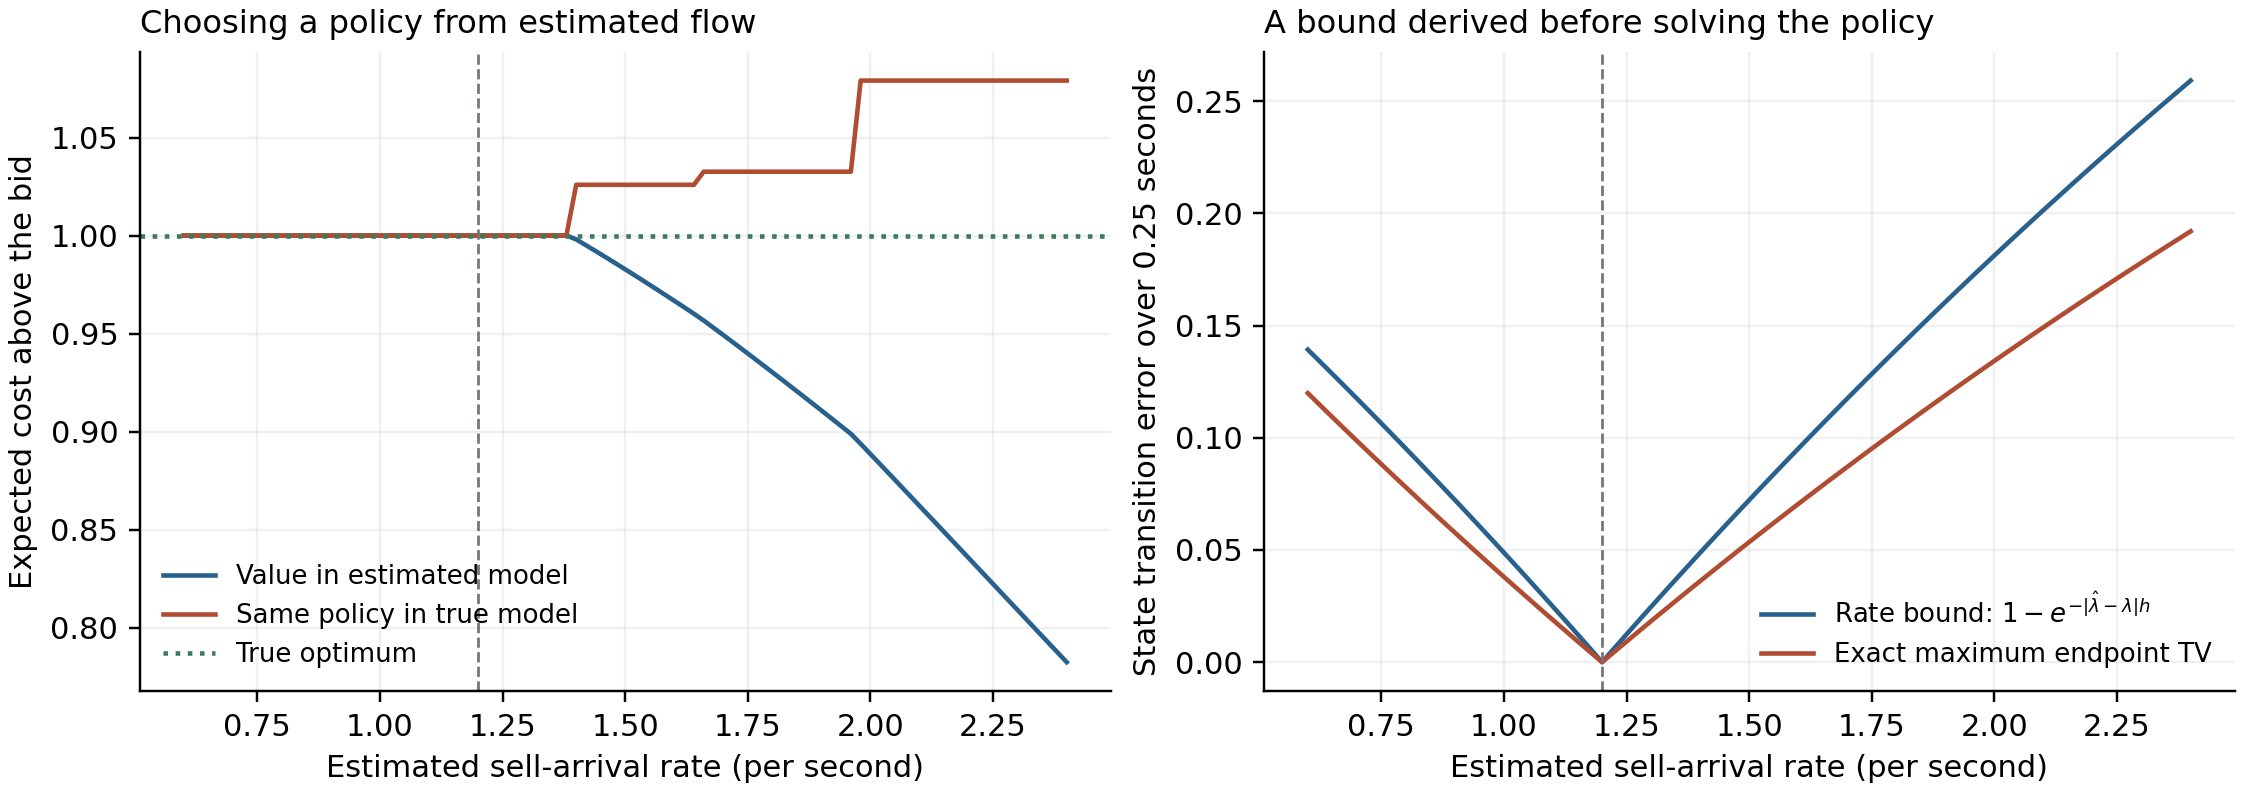
\includegraphics[width=\textwidth]{figures/09_orderbook_bridge.png}
\caption{The order-flow construction and its consequences. Left: the value
of each learned policy in its fitted environment and its cost when deployed
unchanged in the true synthetic model. Right: exact maximum state-endpoint
total variation over $0.25$ seconds and its primitive-rate bound. The right
panel measures the state marginal; the theorem also bounds the richer joint
path of states, fills and reports. The dashed vertical line marks the true
sell rate.}
\label{fig:bookbridge}
\end{figure}

Verification covers 3,888 small variable-size matching cases, share
conservation, price priority, an explicit FIFO check, and the equal-depth
counterexample with different own fills. A Poisson-series calculation agrees
with the independently computed matrix exponential to within $10^{-13}$
in maximum row total variation, with its omitted tail recorded separately.
The fixed-policy and regret bounds are checked at every state and remaining
decision time for seven estimated rates, giving 532 state--stage--model
comparisons. Separate matrix calculations verify the stationary response
remainder for constant and piecewise signed inputs and the exact two-state
exponential response. The proofs establish the general statements; these
checks establish the stated numerical implementation and expose its finite
state, atomic-cancellation and guaranteed-terminal-liquidity assumptions.

\subsection{Feasible signature feedback with a computed optimization bound}
\label{sec:feedbackexperiment}

A further experiment implements \cref{prop:finitesoftmax} in the same
19-state book. The state is fully observed in this specialization. The
report alphabet may therefore include the post-event state, and a based
state-indicator channel has first-level signature $e_{S_{t_k}}$ at each
decision. The stage-specific logit coefficients assign score $r$ to the
Bellman-optimal action in each observed state and score zero to the other
admissible actions. Crossing an empty ask receives exactly zero probability
through the mask; after completion only a no-operation action is retained.
This is an implemented signature-softmax policy, rather than an unexecuted
proposal for a policy class.

For $K=4$, $L=2$ and at most three actions,
\cref{prop:finitesoftmax} gives the global approximation bound
\begin{equation}\label{eq:feedbacktaunumerical}
 \tau(r)=\min\{2,16/(e^r+2)\}.
\end{equation}
Here the Bellman oracle solves the fully observed finite model. Depth-one
state logits can approximate every deterministic Markov optimizer as
$r\to\infty$, so this class has the same infimum as the full feedback
class. The computed objective gap is checked against \eqref{eq:feedbacktaunumerical}
at every state and remaining decision time. No local training residual is
used as a global optimality certificate.

Table~\ref{tab:feedback} gives two sets of coefficients: one from the true
sell rate $1.2$, and one from the estimated rate $1.4$. Both policies are
evaluated at the true rate $1.2$. The latter satisfy the combined bound
\[
 \min\{2,\ 4(1-e^{-0.2})+\tau(r)\}.
\]
Increasing $r$ removes the softmax approximation error. Under the correct
model, regret tends to zero; under rate misspecification it approaches the
previous deterministic-policy regret of approximately $0.025897$.
Model error and policy approximation have distinct effects even in this
small example.

\begin{table}[tb]
\centering\small
\caption{Depth-one signature feedback in the fully observed synthetic book.
Regrets use the true rate $1.2$ and initial state of \cref{sec:bookexperiment}.
The two coefficient sets are constructed by finite backward induction at
rates $1.2$ and $1.4$. Bounds hold before rounding.}
\label{tab:feedback}
\begin{tabular}{rrrrr}
\toprule
$r$ & Correct-model regret & $\tau(r)$ & Misspecified regret & Combined bound\\
\midrule
\inputtable{tables/feedback_rows.tex}
\bottomrule
\end{tabular}
\end{table}

The new verification script reconstructs 31 finite transcripts, distinguishes
initial observations and co-timestamped report order, and checks 1,260
flooring, finite-score and exact-mask cases. It evaluates 14 signature
policies, checks 1,064 state--stage optimization comparisons and 1,064
consecutive-hybrid comparisons under the laws of earlier replacement
policies. It also verifies the frozen-mode counterexample and 256
finite-policy comparisons with an autonomous reference model. The latter
checks concern the terminal state marginal; the full-path estimate is
established by the coupling proof. All these are finite synthetic checks,
not a numerical proof of the general Lusin approximation, a generic depth
complexity result, or an empirical execution study.

\subsection{A certified controller with hidden, action-dependent liquidity}
\label{sec:partialexperiment}

This experiment implements \cref{thm:computablepartial,prop:partialmeshrate,cor:partialsignature}.
The controller does not observe the liquidity regime,
and its actions change the future regime and its reports. Every optimality
bound below is a finite-model calculation. The model is synthetic, with no
calibration or claim about realized exchange performance.

\subsubsection*{Model, information and feasibility}

The parent is 1,000 shares, represented by $q_0=10$ units of 100 shares,
with $K=12$ decisions. Hidden liquidity is $H_k\in\{0,1\}$, good or bad,
with initial probability $b_0=1/2$ of bad liquidity. At each decision an
instruction specifies an immediate market quantity $m_a$ and a passive
quantity $\ell_a$, in these units. Feasibility requires
$m_a+\ell_a\le q_k$. Unfilled passive interest expires before the next
decision; completed parents have only a no-operation action.

After action $a$, the hidden regime transitions according to $T_a$.
Conditional on $H_{k+1}=h'$, the passive fill is
$F_{k+1}\sim\operatorname{Binomial}(\ell_a,p_{a,h'})$ and a public binary
signal $Y_{k+1}$ is independent of that fill, with
\[
 \Pp(Y_{k+1}=1\mid h'=0)=0.35,\qquad
 \Pp(Y_{k+1}=1\mid h'=1)=0.65.
\]
The controller observes its action, own fill, public signal and resulting
quantity $q_{k+1}=q_k-m_a-F_{k+1}$. It does not observe $H_{k+1}$.
Table~\ref{tab:partialparameters} specifies all action-dependent probabilities.
The labels \emph{lit} and \emph{dark} name stylized passive alternatives, not an
implementation of a venue's native allocation rules.

\begin{table}[tb]
\centering\small
\caption{Synthetic controlled-liquidity parameters. Transition and fill
entries are probabilities; the final column is a per-instruction USD fee.
$T_{01}$ is good-to-bad and $T_{10}$ is bad-to-good.}
\label{tab:partialparameters}
\begin{tabular}{lrrrrrr}
\toprule
Action & $(m_a,\ell_a)$ & $T_{01}$ & $T_{10}$ & $p_{a,0}$ & $p_{a,1}$ & $\varphi_a$\\
\midrule
Wait & $(0,0)$ & .05 & .18 & 0 & 0 & 0\\
Lit 1 & $(0,1)$ & .12 & .12 & .80 & .18 & .010\\
Lit 2 & $(0,2)$ & .28 & .07 & .65 & .08 & .010\\
Dark 1 & $(0,1)$ & .04 & .15 & .70 & .03 & .025\\
Market 1 & $(1,0)$ & .35 & .06 & 0 & 0 & 0\\
Market 2 & $(2,0)$ & .60 & .03 & 0 & 0 & 0\\
Split 1+1 & $(1,1)$ & .40 & .05 & .72 & .12 & .010\\
\bottomrule
\end{tabular}
\end{table}

For $o=(f,y)$, the primitive finite kernel is
\begin{equation}\label{eq:partialexperimentkernel}
 M_{q,a,(f,y)}(h,h')=
 T_a(h,h')\binom{\ell_a}{f}p_{a,h'}^f(1-p_{a,h'})^{\ell_a-f}
 z_{h'}^y(1-z_{h'})^{1-y},
 \quad (z_0,z_1)=(.35,.65).
\end{equation}
The stage loss and terminal completion charge, in USD, are
\begin{align}\label{eq:partialexperimentcost}
 c(q,a,f)&=m_a+0.18m_a^2+0.08f+\varphi_a
                      +0.04(q-m_a-f)^2,\\
 c_K(q,h)&=1.8q+0.15q^2.\nonumber
\end{align}
The terminal facility fills every remaining share at this stipulated charge.
It is part of the synthetic feasibility model. The cost separates immediate
execution, passive-fill charges, instruction fees and an inventory penalty.

The hidden law is substantially action dependent. Before observing the next
report, a prior of $1/2$ leads to bad-state probability $0.435$ after waiting
and $0.785$ after a two-unit market order. Those probabilities are generated
by the transition matrices, independently of any belief update. A controller
that treats the hidden process as unaffected by trading solves a different
decision problem.

\subsubsection*{Computed global gaps and their interpretation}

The implementation solves both finite recursions for
$m=8,16,\ldots,1024$ subintervals and evaluates each selected table in the
physical hidden-state model. It does not simulate by resampling a regime
from its rounded belief. The initial prior is exactly a grid node in every
case. Table~\ref{tab:partialgrid} reports a lower bound on the optimum over
all policies using the specified observations and an upper enclosure of the
deployed controller's expected cost.

\begin{table}[tb]
\centering\small
\caption{Global certificates under partial observation, in USD. Value
endpoints are displayed outward to eight decimals. Gaps are computed from
the unrounded enclosures and displayed upward; they need not equal the
difference of the displayed value endpoints.}
\label{tab:partialgrid}
\begin{tabular}{rrrr}
\toprule Belief nodes & Optimal-value lower bound & Controller-cost upper bound & Certified gap\\
\midrule
\inputtable{tables/partial_grid_rows.tex}
\bottomrule
\end{tabular}
\end{table}

With 1,025 belief nodes, the optimum is enclosed between
\$\PartialLower\ and \$\PartialValue, and the controller's certified gap
is at most \$\PartialGap. These small numbers measure planning error within
the exact synthetic model; they are not precision claims about market costs.
The elementary stage-range bound gives $S_j=33+5.28(12-j)$ and a uniform
mesh guarantee of approximately \$1.09055 at the finest grid. The much
smaller computed certificate makes the decision comparison informative.

The deployed policy does not improve monotonically with every refinement:
the 17-node policy is slightly more expensive than the 9-node policy, and
the 65-node policy is slightly more expensive than the 33-node policy.
The certificate, rather than an adjacent-grid difference, determines when
the achieved accuracy is adequate. The 257-node case already has a gap
below \$0.000007.

\begin{figure}[tb]
\centering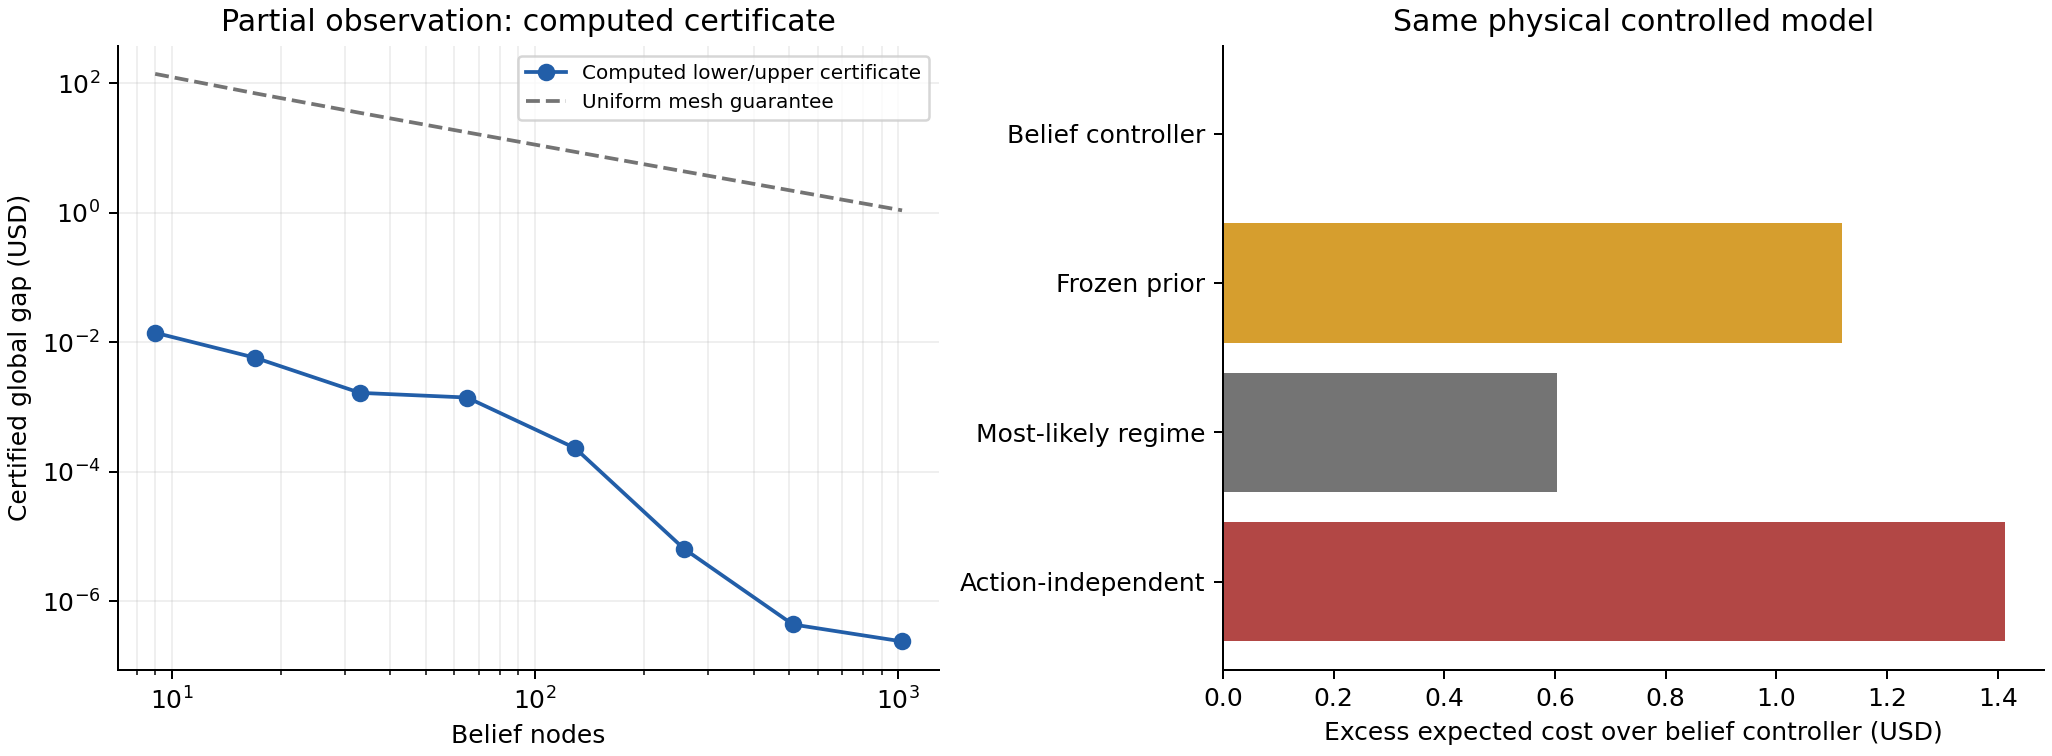
\includegraphics[width=\textwidth]{figures/10_partial_observation_certificate.png}
\caption{Computed global planning certificates and comparisons in the same
controlled hidden-liquidity model. The uniform mesh bound is deliberately
conservative. The right panel compares physically evaluated expected costs;
no hidden-state observation is supplied to these four controllers.}
\label{fig:partialcertificate}
\end{figure}

\subsubsection*{Decision comparisons and finite signature implementation}

The frozen-prior baseline solves a finite dynamic program which resets its
belief to the initial prior after each report, while retaining $T_a$ in
each one-step prediction. It is then evaluated under the persistent physical
regime. The most-likely-regime baseline filters the reports and applies the
fully observed Bellman action for the more probable regime, with a fixed
tie rule. The action-independent-transition baseline plans and filters with
$T_a=T_{\rm wait}$ for every action, retaining the action-specific fill
probabilities, and is evaluated under the true action-dependent matrices.
All three have the same instruction set, loss and completion facility.
The first and third are explicitly specified misspecified-model baselines,
not claims to optimality over every controller that omits information.

\begin{table}[tb]
\centering\small
\caption{Physical-model policy evaluation, in USD. Costs are rounded upward;
excess costs are conservative lower bounds relative to the certified belief
controller. Baseline definitions are given in the text.}
\label{tab:partialpolicies}
\begin{tabular}{lrr}
\toprule Policy & Expected-cost upper bound & Excess-cost lower bound\\
\midrule
\inputtable{tables/partial_policy_rows.tex}
\bottomrule
\end{tabular}
\end{table}

At the stated initial condition, the belief controller lowers expected
objective by approximately \PartialFrozenPct\% relative to the frozen-prior
baseline and \PartialBlindPct\% relative to the action-independent-transition
baseline. A fully observed regime oracle has expected cost
\$\PartialOracle. Its lower cost reflects extra information and is not the
partially observed optimality benchmark used in the certificate.

The preferred-action table is then converted to the finite-score signature
controller of \cref{cor:partialsignature}. The preferred action has weight
$w$ and every other admissible action has weight one. Table~\ref{tab:partialsoft}
evaluates this randomized controller itself, including its effects on future
liquidity and beliefs. For $w=2^{20}$, its certified global gap is at most
\$\PartialSoftGap. The result therefore covers an implemented finite-score
policy rather than only a deterministic limit with infinite logits.

\begin{table}[tb]
\centering\small
\caption{The implemented finite-score signature controller, using 1,025 belief
nodes. The preferred score is $\log w$; other feasible scores are zero.
Costs and gaps are in USD and displayed upward.}
\label{tab:partialsoft}
\begin{tabular}{rrr}
\toprule Preferred weight $w$ & Expected-cost upper bound & Certified global gap\\
\midrule
\inputtable{tables/partial_softmax_rows.tex}
\bottomrule
\end{tabular}
\end{table}

\begin{figure}[tb]
\centering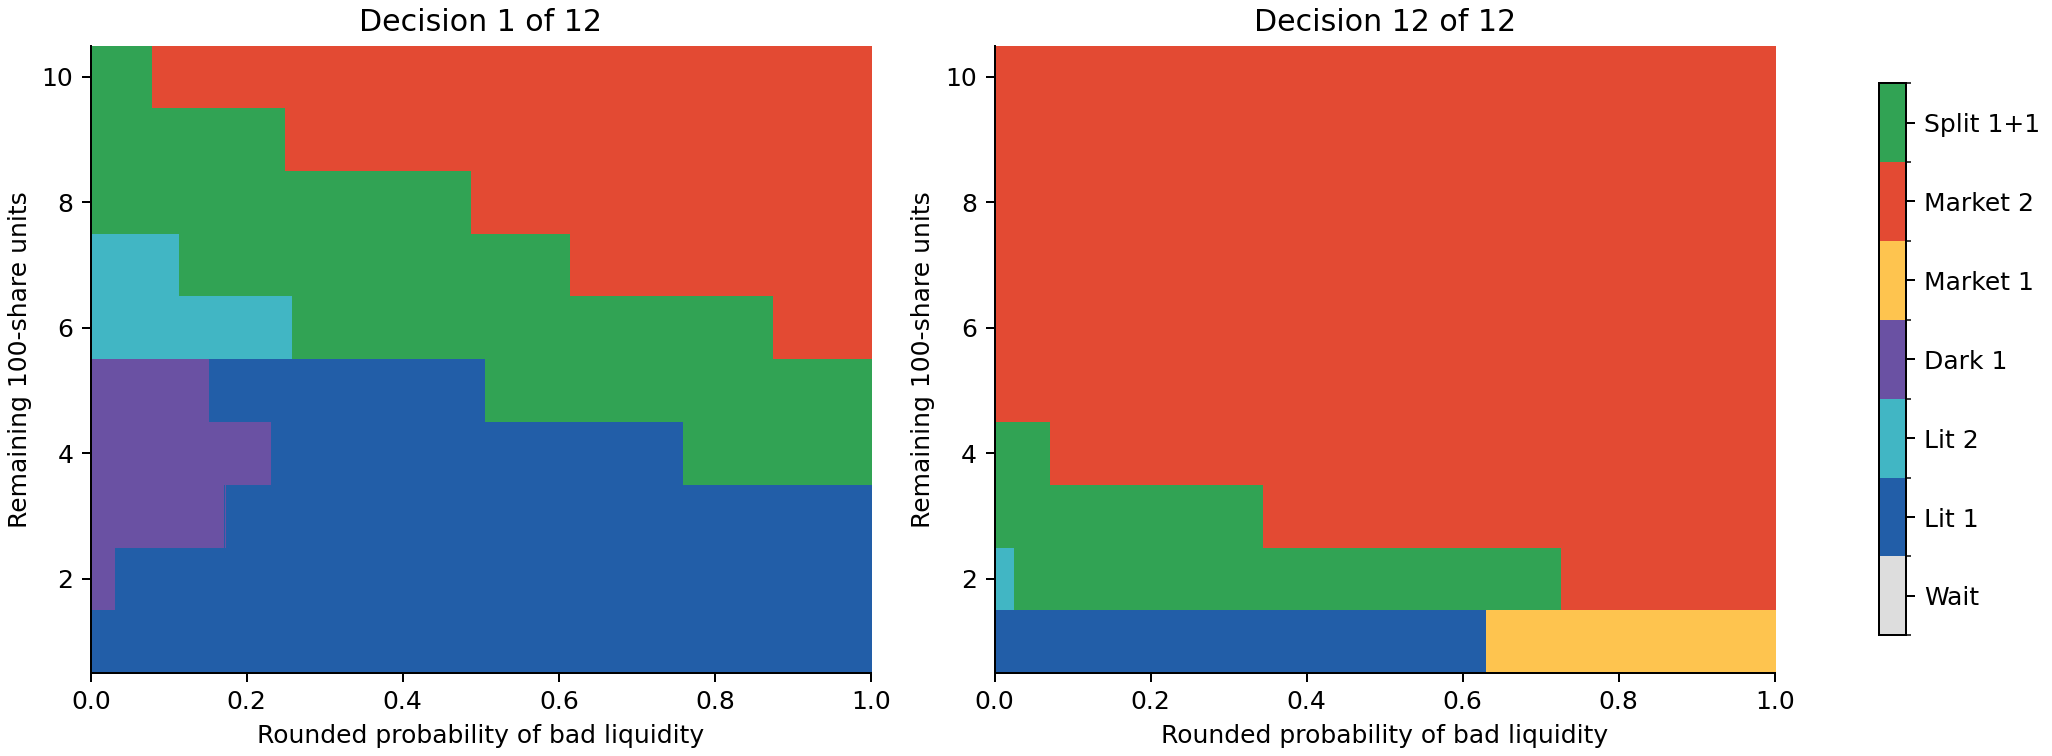
\includegraphics[width=\textwidth]{figures/11_partial_observation_policy.png}
\caption{Preferred instructions at the first and last decisions as a function
of remaining quantity and observable rounded belief. The hidden regime is
not an input. The policy table is encoded by the endpoint of the finite
observable summary channel.}
\label{fig:partialpolicy}
\end{figure}

\subsubsection*{Sensitivity and independent verification}

The same fixed economic parameters are also tested with six or twelve
decisions and initial bad-state probabilities $1/4,1/2,3/4$, using 257 belief
nodes. Table~\ref{tab:partialrobust} reports all six combinations. The belief
controller improves on both specified baselines in every case, although
the benefit varies substantially with prior and deadline. This is a
sensitivity check of the declared model, not evidence of universal superiority.

\begin{table}[tb]
\centering\small
\caption{Prior and deadline sensitivity. All USD columns use outward rounding.
The last two columns give lower bounds on baseline excess cost over the
certified controller. Every row uses 257 belief nodes.}
\label{tab:partialrobust}
\begin{tabular}{rrrrrr}
\toprule $K$ & $b_0$ & Controller cost & Global gap & Frozen-prior excess & Transition-blind excess\\
\midrule
\inputtable{tables/partial_robustness_rows.tex}
\bottomrule
\end{tabular}
\end{table}

All primitive probabilities in \eqref{eq:partialexperimentkernel} are integer
multiples of $10^{-8}$. For grid beliefs, posterior numerators and
nearest-node decisions are computed with integer arithmetic, including
ties. Elementary nonnegative products, sums and divisions in the bound
recursions are enclosed by outward expansion using the adjacent binary64
floating-point numbers. The value enclosures are approximately
$1.2\times10^{-13}$ USD wide; the global finite-grid optimization tolerance
from \eqref{eq:partialnumericalgap} is below $1.2\times10^{-12}$ USD.
The reported policy-approximation gaps are separate from these numerical
enclosure widths.

An independent exact-rational exhaustive recursion for three decisions and
two units gives
\[
 V^*=\frac{232172138011}{156250000000}=1.4859016832704.
\]
Its 3,553 distinct recursion states give a value between the grid lower bound
and the controller upper bound. Exact-rational evaluation of the deterministic
and finite-score controllers is also contained in the corresponding outward
intervals. A separate forward occupancy calculation agrees with the main
backward physical evaluation to better than $10^{-10}$ USD, conserves total
probability to better than $10^{-12}$, and visits 9,390 positive-probability
stage/memory states. The code checks 24,600 integer posterior-rounding and
probability-enclosure cases on the finest grid.

These computations are reproducible without an optimization oracle or a
Monte Carlo stopping criterion. They certify global planning accuracy for
the stated finite-observation model. Transfer to an estimated market model
still requires a justified $B_T$ in \eqref{eq:partialtransfer}; increasing
belief resolution cannot compensate for incorrect transition, reporting or
cost assumptions.


\subsection{Exact checks of the cost of discarded reports}
\label{sec:summaryexperiment}

The finite-observation planning gap and the loss of an omitted observation
are different quantities. This experiment checks
\cref{thm:summarysandwich,prop:binarysummary} on a finite tree where both can
be evaluated exactly. It also shows why a fine belief grid cannot recover
information that the controller never receives.

\subsubsection*{Controlled liquidity with a coarser controller}

Use the seven instructions, transitions, fills and charges in
\eqref{eq:partialexperimentkernel}--\eqref{eq:partialexperimentcost}, with
three decisions, two quantity units and $b_0=1/2$. The richer agent observes
both the fill and public signal. The implemented summary controller retains
the quantity and a rounded filter driven only by fills; it discards the
public signal. Its update uses the kernel obtained by summing
\eqref{eq:partialexperimentkernel} over $y$. It retains the same exact
quantity mask as the richer agent.

All positive-probability fine-report histories under all feasible actions
are enumerated with rational arithmetic. Histories are merged only when
their stage, quantity, controller memory and exact full posterior agree.
At each summary, the smallest and largest of these full posteriors give
\eqref{eq:posteriorfiber}. The endpoint recursions then produce $L,U$ and
the upper-recursion minimizing policy $\sigma$. Independently, full-posterior
dynamic programming computes $V^{\rm rich}$, and fill-history dynamic
programming computes the exact coarse-history optimum $V^{\rm coarse}$.
The latter retains the entire fill history and has no rounding error.
A separate forward calculation propagates actual hidden-state probabilities
under the fixed $\sigma$ to obtain its physical cost $J_\sigma$.

\begin{table}[tb]
\centering\small
\caption{Exact finite-tree observation-reduction checks, in USD.
$z_0/z_1$ denotes the two probabilities of public signal one given next
hidden state; $m$ is the number of uniform belief subintervals.
The two exact optima and $L_0$ are displayed downward to six decimals;
$J_\sigma$ and $J_\sigma-L_0$ are displayed upward. The machine-readable
results retain every exact rational value.}
\label{tab:summarycertificate}
\begin{tabular}{rrrrrrr}
\toprule
$z_0/z_1$ & $m$ & $V^{\rm rich}$ & $V^{\rm coarse}$ &
$J_\sigma$ & $L_0$ & Certified gap\\
\midrule
\inputtable{tables/observation_summary_rows.tex}
\bottomrule
\end{tabular}
\end{table}

The first row uses the original public-signal probabilities. Its richer
optimum is the previously checked
$232172138011/156250000000=1.4859016832704$.
Discarding the signal raises the optimal expected cost by exactly
$1293658149/156250000000=0.0082794121536$ USD, before any rounding or
summary-policy restriction. The remaining rows strengthen only the report,
to probabilities $0.05$ and $0.95$. The coarse model is unchanged because
it integrates out that report. Its information loss rises to exactly
\[
 V^{\rm coarse}-V^{\rm rich}
 =\frac{205859933299369}{2500000000000000}
 =0.0823439733197476\ \mathrm{USD}.
\]
Increasing $m$ from eight to sixteen slightly improves the
certificate while leaving the selected controller's initial cost unchanged.

These are valid but conservative certificates: the stagewise interval
extrema can combine posterior histories that one physical trajectory cannot
jointly realize. The upper-recursion policy need not be optimal among
summary policies. The reported gap uses the sharper physical evaluation
$J_\sigma-L_0$, not $U_0-L_0$, and is compared with the exact achieved gap
$J_\sigma-V^{\rm rich}$ in the audit output.

There are $1,24,324,3456$ distinct full-posterior/memory states at the four
stages in each case. Every one of the 349 nonterminal states satisfies
$L\le V^{\rm rich}\le J^\sigma\le U$ in exact arithmetic. The separate
forward hidden-state evaluation equals the history-based evaluation exactly
and conserves probability at every stage. The maximum discrepancy between
the full posterior and rounded memory exceeds $0.43$ even in the first
case, whereas the one-step rounding radius is $1/16$. This directly checks
that those two errors cannot be identified.

\subsubsection*{A transparent probe example and the sufficiency limit}

For a separate two-decision example, one unit remains and good/bad liquidity
is static with equal prior probabilities. At the first decision the trader
may wait at zero cost or pay $0.02$ USD for a report that identifies the
state correctly with probability $0.9$. At the second decision, a market
instruction completes at cost $1$ USD. Alternatively, a passive instruction
fills at zero cost with probability $0.9$ in good liquidity and $0.1$ in bad
liquidity; any failure is completed at cost $2$ USD. Every instruction is
feasible and all residuals are completed.

Writing $b$ for the probability of good liquidity in this example, the
passive expected cost is $1.8-1.6b$. A retained favorable report gives
$b=0.9$ and passive cost $0.36$; an unfavorable report gives $b=0.1$ and
selects the market instruction. Thus the richer agent probes and has value
\[
 V^{\rm rich}=0.02+\tfrac12(0.36+1)=0.70.
\]
An agent discarding the report has exact posterior $b=1/2$, optimally waits,
and has value $V^{\rm coarse}=1$. Its information loss is $0.30$ USD even
with an exact coarse filter and no quantization. If the summary remembers
whether it probed but discards the report, its post-probe posterior envelope
is $[0.1,0.9]$. The endpoint recursions give
\[
 L_0=\min\{1,0.02+0.36\}=0.38,\qquad
 U_0=\min\{1,0.02+1\}=1.
\]
The resulting $0.62$ USD certificate covers the $0.30$ USD actual loss.
Retaining the report makes every conditional envelope a singleton; both
recursions then equal $0.70$, as required by
\cref{cor:summarysufficiency}. These values are checked as exact fractions.

\subsubsection*{Action certificates and decision sufficiency}

The same three finite trees also check
\cref{thm:summaryactioncertificate}. Every one of the 1,237 feasible
state--action pairs per case satisfies both action bounds in
\eqref{eq:summaryactionbounds} and the Bellman-advantage bound
\eqref{eq:summaryactionexcess}, using exact fractions. The resulting regret
recursion bounds the selected controller at all 349 nonterminal states.
Across the three cases, 648, 409 and 417 strict action-screening comparisons
identify only truly suboptimal actions. These counts include the different
full histories in a common summary fiber.

\begin{table}[tb]
\centering\small
\caption{Two certificates for the same implemented controller in the
three controlled-liquidity cases, in USD. The cost certificate is
$J_\sigma-L_0$ using physical evaluation; the action certificate is
$R_0^\sigma$. The combined bound takes their minimum. All displayed gaps
and bounds are rounded upward to six decimals from exact rational values.}
\label{tab:actioncertificate}
\begin{tabular}{rrrrrr}
\toprule
$z_0/z_1$ & $m$ & Actual gap & Cost certificate & Action certificate & Combined\\
\midrule
\inputtable{tables/action_separation_rows.tex}
\bottomrule
\end{tabular}
\end{table}

Here the cost certificate is sharper in every row of
\cref{tab:actioncertificate}; the action recursion is not a uniformly
tighter replacement. A separate two-stage case shows the distinction.
At the first stage the only feasible action costs $0.02$ USD and produces
a perfect report of a static, equally likely binary state. The richer agent
retains this report and the summary controller discards it. At the second
stage both terminal instructions complete the remaining unit by assumption.
Instruction $L$ has all-in charges $0.10$ and $0.20$ USD in the two states;
instruction $M$ costs $0.50$ USD in either state. These supplied charges
define a finite execution example, not an estimated exchange fill law.

The summary's posterior envelope after the report is $[0,1]$. Its action
bounds are $Q^-(L)=0.10$, $Q^+(L)=0.20$ and
$Q^-(M)=Q^+(M)=0.50$. Hence $e(L)=0$ and $e(M)=0.40$.
The fixed controller choosing $L$ has
\[
 L_0=0.12,\qquad J_L=V_0^{\rm rich}=0.17,\qquad U_0=0.22.
\]
The physically evaluated cost certificate is $0.05$ USD, but the action
certificate is exactly zero. It establishes optimality despite the
non-singleton envelope and nonzero cost interval. The richer conditional
value at the final decision is $0.10$ or $0.20$, so the summary is
\emph{decision sufficient} here without determining that conditional value.

For a randomized controller choosing $M$ with probability $1/4$, physical
cost is $0.2575$ USD and true regret is $0.0875$ USD. The cost certificate
is $0.1375$ USD while the action certificate is $0.10$ USD. The script
checks these quantities and the conditional bounds in both hidden states
as exact fractions. This also checks the action average in
\eqref{eq:summaryactionrecursion}; randomization is evaluated as implemented.

The script \texttt{scripts/observation\_summary\_checks.py} generates both
tables and stores the exact fractions, state counts and conditional checks.
The same script checks the Gaussian sign symmetry in
\cref{thm:ledgerlower} and the nonuniform cell created by inserting the
initial prior $1/3$ into an eight-subinterval grid. These are finite
verification cases supporting the written proofs; they do not constitute a
machine-checked proof of the general conditional-envelope theorem.


\clearpage
\part{Implementation and evidence}\label{pt:impl}
\section{Learning a model suitable for execution}\label{sec:learning}

\subsection{The target is an action-dependent joint law}

The marked construction in \cref{sec:bookbridge} gives a concrete route:
learn the action-dependent primitive intensities and any unidentified mark
law, apply the specified matching and reporting maps, and compose the joint
interval kernel. Known matching rules constrain the outputs, while the
uniform primitive-error condition remains a separate statistical requirement.
Good likelihood fit on the logging distribution alone does not establish it.

A generative model for displayed books can learn
$p(B_{t+1}\mid B_{\leq t},\text{observed flow})$. An execution optimizer needs
more: the response to the trader's order and the joint distribution of fills,
prices, costs and reports. Its target is of the form
\begin{equation}\label{eq:jointlearn}
 p_\theta(F,P,Y,B',\ell',I',r'\mid B,\ell,I,r,b,a).
\end{equation}
Generating statistically plausible future books without conditioning on the
action is insufficient for evaluating a policy that materially changes demand,
queue composition or information disclosure.

An LSTM variational autoencoder can compress history; a transformer can model
longer event dependencies or interactions between venues. Their embeddings
are useful only insofar as they support the relevant conditional law. A latent
coordinate should not be named ``true hidden inventory'' unless there is an
identification argument or appropriate ground truth. A model can use a latent
state to represent uncertainty without claiming the state is physically
measured reserve size.

For displayed geometry, one can encode a reference price, positive spread,
positive interlevel gaps, total depth, depth composition and order counts.
Log or softplus coordinates enforce positivity; log-ratio coordinates represent
compositions. Decoding must respect tick grids and integer quantity constraints.
Hidden executions can use a finer price grid than displayed quotes, including
midpoint prices. These transformations help produce valid states. They do not
by themselves enforce the parent quantity, exchange priority, causality or
correct joint fill/return dependence.

\subsection{Observation, mechanism and policy models}

It is useful to distinguish three fitted objects. The observation model maps
latent states and actions into the data the trader can see. The mechanism model
maps orders and market events into fills and state changes. The policy maps
the resulting state or belief into admissible instructions. Their errors have
different consequences. A book forecast can be accurate while its implied
fill model is wrong; an exact accounting engine can conserve shares while its
arrival intensities are unrealistic; a correct simulator can still be used
by a poorly optimized policy.

When all required mechanisms are observed, the book/queue engine should apply
the rule directly. When priority, reserve attribution or far depth is unobserved,
it should expose a distribution or bounds. Fabricating a deterministic queue
position, matching all depth decreases to trades, or inserting a one-share
tail beyond the observed book replaces missing information with unsupported
liquidity.

The finite-state belief approach traces back to partially observed control
\citep{smallwood1973}. In a large model, particle filters, variational filters
or recurrent sufficient-state approximations can replace the finite posterior.
The action must remain an input to the update. A fixed filter trained only
on passive observations may be miscalibrated when an aggressive execution
policy changes the observation process.

\subsection{Impact and counterfactual response}

For transient impact, a simple additional state is
\begin{equation}\label{eq:impactstate}
 I_{k+1}=\rho I_k+\zeta x_k,\qquad 0\leq\rho<1,\quad\zeta\geq0,
\end{equation}
where $\zeta$ is the impact-state loading per executed share, distinct from
the permanent coefficient $\gamma_{\rm p}$. Specify the relationship between
$I_k$, execution premiums and observed
prices. Persistent impact makes an early venue choice influence later costs.
Cross-venue or cross-asset impact requires an appropriately coupled state.
The chosen impact structure should be checked for unintended profitable
round trips, a central issue in the market-impact literature
\citep{gatheral2010,schneider2019}. A generic neural price generator does not
automatically satisfy such restrictions.

Historical replay answers a restricted question: what would a sufficiently
small, non-disruptive order have encountered under a modeled queue assumption?
It cannot reveal with certainty the counterfactual response to a different
large order. Estimating impact requires suitable variation in action size,
timing and market conditions, with controls for the information that drove
those actions. Otherwise, a measured post-trade price change can mix impact,
selection and common news.

\section{From optimization to executable messages}\label{sec:algorithm}

A practical controller uses receding-horizon optimization. At each reliable
decision point it updates its state, simulates or integrates candidate
continuations, sends the first admissible instruction, and then incorporates
the resulting reports before replanning. Optimization frequency should reflect
the event rate, computation budget and value of changing a decision. Faster
replanning is not useful if it repeatedly forfeits queue position or acts on
stale observations.

\begin{center}
\fbox{\begin{minipage}{.94\textwidth}
\textbf{Execution controller at one decision point}
\begin{enumerate}
\item Incorporate sequenced market events and authoritative order reports;
      reject duplicated fills and retain unresolved exposure.
\item Update reference prices, book coverage, session/auction phase,
      remaining quantity and each child's reservation.
\item Update liquidity and queue beliefs using the actions actually sent
      and the observations that have become available.
\item Form the admissible actions from quantity, price, NYSE/Nasdaq
      destination, native order instruction, participant access, lifetime
      and mandate constraints.
\item Evaluate joint fill/price scenarios and continuation values, including
      terminal feasibility, risk and model uncertainty.
\item Choose a first action, reserve its maximum possible exposure, and send
      the instruction with a unique identifier.
\item Replan after new information or a scheduled decision time. Release
      capacity only after authoritative execution or terminal cancellation.
\end{enumerate}
\end{minipage}}
\end{center}

The optimization can use convex scheduling, dynamic programming, mixed-integer
programming, scenario trees, or a learned policy. The choice depends on which
state dimensions and constraints matter. Reinforcement learning is a possible
solver for the same declared objective, not a substitute for defining it.
Hard quantity and instruction restrictions should be enforced by construction
or an admissibility layer; a reward penalty alone does not guarantee them.

The planner must distinguish a requested cancel from a confirmed cancel,
a route instruction from an execution, and a venue acknowledgment from a
fill. Message arrival order can differ from event time. Market data and private
execution reports also have different clocks and sequencing conventions.
Nasdaq ITCH and OUCH describe public market data and the participant's own
order lifecycle, respectively; NYSE Pillar FIX describes the NYSE order-entry
and execution-report channel \citep{itch,ouch,nysefix}. A feed decoder should
not invent private lifecycle events absent from public data.

\subsection{A two-exchange implementation}

The practical interface has four components: a parent scheduler, a NYSE adapter,
a Nasdaq adapter, and an authoritative commitment ledger. Each adapter validates
native instructions and returns a joint law for acceptance, fills, prices and
reports. The scheduler requests execution subject to the mandate; it does not
assume that a requested rate is delivered by a passive order. Child orders at
both destinations draw from the same parent reservation budget.

For example, a patient buy can compare resting displayed interest with a
supported hidden or midpoint instruction on either exchange. When the
conditional cost of missing the deadline rises, marketable limits or IOC
instructions may become preferable. Approaching the primary closing auction,
the controller compares a valid auction commitment with continuous completion.
This is a policy comparison within the specified state and access constraints,
not a fixed ranking of NYSE versus Nasdaq. Correlated fills, fees, adverse
selection and lost cancellation flexibility belong in that comparison.

\subsection{Causality and latency}

Let $\tau_e$ be matching-engine event time and $\tau_r$ the time an event becomes
available to the controller. The policy filtration uses $\tau_r$, together
with completion/sequence rules needed to interpret the event. It cannot
condition on an event merely because $\tau_e$ precedes the decision timestamp.
Similarly, a new order sees the book at its arrival, not necessarily the book
observed when it was sent. A latency model should couple arrival-time depth,
price movement and cancellations rather than attach an independent constant
slippage to every route.

Latency can be economically asymmetric. It changes the chance of receiving
an attractive displayed quote, the chance of canceling before an adverse
execution, and the value of waiting for more information. These effects can
change the optimal order type even when expected price drift is unchanged.

\section{What would constitute market evidence?}\label{sec:validation}

\subsection{Data requirements matched to the claim}

\begin{table}[tb]
\centering\small
\caption{The evidence required grows with the strength of the execution claim.}\label{tab:evidence}
\begin{tabularx}{\textwidth}{YY}
\toprule Claim & Required evidence \\\midrule
Displayed-book prediction & Causal book states, quality flags, chronological splits and calibrated distributional scores \\
Passive fill prediction & Private order lifetimes/fills or defensible queue replay, cancellations, censoring and latency \\
Reserve inference & A validated observation model, native identities or private order evidence where available, and sensitivity to non-identification \\
Auction execution & Imbalance/statistics/status feeds, accepted order commitments, allocation and effective cutoff rules \\
Cross-venue routing & Synchronized relevant books/references, route and execution logs, fee eligibility and joint fill dependence \\
Large-order impact & Data supporting counterfactual response estimates, with action selection and market conditions addressed \\
Policy improvement & Comparable mandates, costs, residual treatment, tail outcomes and an evaluation design supporting the policy comparison \\
\bottomrule
\end{tabularx}
\end{table}

Data selection should follow the intended claim. Market-by-price data provide
aggregate price-level states. Market-by-order data preserve more of the
displayed order lifecycle, but does not reveal all hidden orders or investor
inventory. Auction statistics, imbalance and status supply different channels.
Even a full displayed book at one exchange is not the national market. A
faithful decoder must respect native message types, execution identifiers and
printability flags to avoid counting one execution more than once \citep{itch}.

\subsection{Evaluation of forecasts and decisions}

Forecast diagnostics should cover fill-size distributions, time-to-fill,
non-fill probability, conditional markouts and dependence across venues.
Book energy scores or price CRPS remain useful for their own targets but
cannot establish execution accuracy. Queue depletion, cancellation survival,
replenishment and auction allocations require separate checks.

Policy diagnostics should include arrival-price shortfall or the specified
benchmark loss, total charges, completion probability, residual size, tail
cost, participation, market impact, and message intensity. Report conditional
results by spread, volatility, time of day, order size, venue and liquidity
regime. A lower mean cost can conceal larger non-completion risk or a worse
tail, so the same mandate must be applied to every comparator.

Useful baselines include rounded TWAP, causal volume schedules, participation
with a completion rule, immediate execution, a calibrated parametric scheduler,
and a simple queue-aware order-placement policy. A neural controller should
earn its complexity against these controls. A reserve-input ablation should
hold targets and training procedures fixed while comparing observed-book
inputs, observable execution flow, and the same inputs with inferred stock.

\subsection{Selection bias and counterfactual policies}

Logged fills are conditional on a historical policy. Orders that were never
submitted have no observed counterfactual fill. Training and evaluating an
alternative policy on those logs therefore require assumptions about support,
state sufficiency and action-dependent response. A replay simulator supplies
one such model; it does not erase selection bias by replaying faster.

For a one-decision problem, a logged-action importance weight is
$w=\pi(a\mid s)/\mu(a\mid s)$, where $\mu$ is the behavior policy. A zero
denominator on actions selected by $\pi$ destroys identification by that
method. Sequential execution compounds the problem because earlier actions
change inventory and observations. Model-based evaluations should state their
counterfactual assumptions; controlled prospective comparisons should retain
mandate constraints and monitor meaningful outcome differences. A random
train/test split of nearby events is not a substitute for chronological
validation across independent dates.

The intended sequence is mechanical verification, distributional calibration,
decision evaluation under stated assumptions, and then appropriately designed
prospective evidence. None of these steps certifies the others. The synthetic
study in Section~\ref{sec:experiments} completes numerical checks within its
declared model; the data-dependent stages remain an empirical research task.

\subsection{Two conditional restrictions and their empirical tests}
\label{sec:testable}

Most evidence requirements in Table~\ref{tab:evidence} are demanding.
Two results nevertheless supply specific restrictions that can be tested
without deploying a counterfactual execution policy. Their data requirements
are identification requirements: public price and trade records alone need
not identify either the strategic trader count or complete metaorders.

\emph{(i) The temporal-skew coefficient.} Under the symmetric game of
\cref{sec:equilibrium}, \cref{thm:crowding} gives
\[
 \Gamma+\tfrac1N\Gamma^*
 =a_N\Sigma+b_N\Lambda,\qquad
 a_N=\frac{N+1}{N},\quad b_N=\frac{N-1}{N}.
\]
The null restriction is $b_N/a_N=(N-1)/(N+1)$, after separating the
temporary-cost term $2\eta I/N$ and fixing the normalization of $\Sigma$
and $\Lambda$. It concerns the equilibrium first-order operator, rather
than the price--flow response kernel. A test therefore needs an identified
common response operator, observed or otherwise identified strategic
participation $N$, and data supporting the symmetric-mandate specification.
\Cref{rem:estimation} lists the main confounds. With those quantities
identified, fit the skew coefficient freely and test the stated equality;
across comparable participation groups, the null also pins down its monotone
dependence on $N$. A raw transaction count is not the strategic trader count
in this model.

\emph{(ii) The joint size-tail restriction.} \Cref{cor:jointtest} links the
impact exponent $\delta$, the metaorder tail index $\alpha$, and the
permanent fraction $c$:
\[
 \delta=\alpha-1,\qquad c=\frac1\alpha.
\]
With identified metaorder sizes and impact paths, estimating $\alpha$ and
$\delta$ freely gives one scalar equality to test. If permanent displacement
is also identified, estimating $c$ adds the second equality.
A comparison using average execution displacement at finite $Q$ must retain
the cutoff correction from \cref{thm:exponent},
\[
 \frac1Q\int_0^Q I(u)\dd u-cYQ^\delta
 =\frac{Y\delta q_0^{1+\delta}}{(1+\delta)Q},
\]
or explicitly specify a different boundary model. The test must distinguish
metaorder size from individual prints and address selection in size, horizon
and liquidity. Inference must account for estimating the exponents, cutoff
and nuisance parameters from dependent observations; the number of scalar
equalities alone does not establish a reference distribution for a test
statistic.

These are tests of combined structural assumptions, and a rejection does not
identify which assumption failed. Neither requires a counterfactual policy
deployment or a replay simulator. Both require suitable trader-level or
metaorder information, or a justified reconstruction and identification model.
They are empirical targets, not tests already performed by the synthetic
experiments in \cref{sec:experiments}.

\clearpage
\part{Outlook}\label{pt:outlook}
\section{Research questions beyond the benchmarks}\label{sec:open}

\begin{enumerate}
\item \textbf{Constrained nonlinear transient execution.} Determine existence,
global optima and quantitative approximation error for a specified nonhomogeneous
response, rate bounds, spread and risk objective. The inequality
$\beta+\delta\geq1$ alone does not settle any of these questions.
\item \textbf{Mechanisms that break scale invariance.}\label{item:scaleinvariance} Test whether observed
size-dependent schedules are explained by rate caps, endogenous horizons,
changing liquidity or nonhomogeneous impact. The homogeneous unconstrained
power-response model itself predicts invariant normalized shape.
\item \textbf{Causal cross-impact estimation.} Estimate matrix kernels under
explicit temporal and round-trip constraints and quantify the effect of the
constraints on out-of-sample execution loss. PSD projection is a known tool;
choosing and identifying the correct causal model is a separate problem.
\item \textbf{Liquidity learning under intervention.} Identify how the trader's
own orders change fills, observations and later depth. Compare a full posterior
with simpler observable state and report decision loss as well as fit scores.
Section~\ref{sec:summarycertificate} supplies the certificate side of that
comparison; the open task is constructing validated posterior envelopes
from realistic reports and timestamps.
\item \textbf{Auction allocation under incomplete observation.} Estimate a joint
law for eligible interest, price, DMM participation and own fills, with effective
NYSE/Nasdaq rules. Public imbalance data alone do not determine all allocation
state or identify investor inventory.
\end{enumerate}

\section{Conclusion}

Execution is the joint choice of quantity over time, instruction and destination
under uncertain completion. Impact benchmarks are useful when their response,
clock, cost convention and feasible strategies are explicit. Linear impact gives
quadratic energy and exact exponential or power-law examples. Nonlinear response
requires separate admissibility and existence analysis; power homogeneity still
fixes size scaling, while a power kernel also changes horizon scaling. A
necessary round-trip restriction is not a certificate for a complete model.

The marginal continuation cost of an unexecuted share connects a schedule to
order placement. Under separable convex costs it yields marginal-cost routing;
with uncertain fills, queue persistence or information effects the choices belong
in a joint dynamic model. Reservations retain exposure until authoritative
reports resolve it. Hidden-liquidity estimates should be judged by their
incremental value for that decision, without equating execution value with price
predictability or latent coordinates with measured investor inventory.

Nasdaq and NYSE auctions require distinct price and allocation representations.
The same public demand/supply totals need not imply the same child-order outcome.
DMM response, order classes, counterpart restrictions, deadlines and residual
opportunities enter the control problem. The worked examples establish their
arithmetic under stated assumptions; the quadratic endpoint model provides an
explicit scheduling benchmark with full fills.

The tagged order-book construction makes the dynamic execution kernel an
output of primitive flow and clearing. It preserves private fills, priority
and the cash ledger; its stationary linear-response limit gives a conditional
propagator representation. Primitive event-rate error then reaches the
execution objective through a common path-coupling bound, alongside the
separate impact-cost error. The resulting certificate does not require an
endogenous book to have the signature model's exogenous quadratic objective.

Within a finite controlled book, complete observable histories and exact
admissibility masks support a vanishing signature policy-class gap. Combined
with uniform model errors and certified global optimization tolerances,
this gives conditional consistency. The explicit finite-state softmax
experiment separates approximation error from persistent model
misspecification. A reference objective has a transferable guarantee only
when its intervention differences and objective-reduction error are
accounted for; an exogenous quadratic identity requires its additional
feature-law and rate-cost assumptions.

For a finite-observation binary hidden model, lower and upper backward
recursions turn that conditional programme into a computable global
certificate. If the deployed controller discards reports, conditional
action-law envelopes give a separate lower bound for the richer-history
optimum. The endpoint construction and exact finite-tree examples show how
to certify this comparison, while the singleton case identifies a sufficient
summary. Coarser information can have a positive cost even with an exact
filter; increasing a belief grid does not remove that loss. Conversely,
an action-separation certificate can establish an optimal instruction even
when the summary does not determine the optimal conditional value.
Obtaining tight, validated envelopes from realistic reports remains a
separate task.

The contribution is a theoretical framework linking impact assumptions to
feasible execution decisions. Its derivations state the conditions under which
schedules, routing rules, information bounds and auction allocations follow.
The numerical comparison illustrates learning within one specified liquidity
model. Empirical calibration and policy evaluation are separate extensions;
they are not needed for the conditional mathematical statements proved here.

\appendix
\section{A continuous-time characterization}\label{app:hjb}

The discrete controller has a continuous-time analogue, with the marked
generator in \eqref{eq:markedcostgenerator} retaining joint fills and price
changes. The following algebra also permits additional continuous dynamics;
its characterization remains subject to the regularity conditions below. Consider a translation-invariant
model whose expected future dollar outlay is $U(t,q,m,z)=qm+v(t,q,z)$.
The state $z$ includes observable market features and a sufficient liquidity
belief. Let the reference midpoint have local drift $\alpha(z)$, and let
$\mathcal L^a$ be the between-event generator for $z$ under passive action $a$.
It includes any belief drift generated by observing no execution.

A passive event has intensity $\lambda_a(z)$ and mark $(f,g,j,z')$, where
$f$ shares execute at premium $g$ per share over the pre-event midpoint,
the midpoint changes by $j$, and the other state changes to $z'$.
After subtracting $qm$, the event's incremental continuation expression is
\begin{equation}\label{eq:jumpcost}
 fg+(q-f)j+v(t,q-f,z')-v(t,q,z).
\end{equation}
This follows by substituting $U=qm+v$ and the recorded cash payment
$f(m+g)$ into the cost-plus-continuation generator. A primitive event can
have $f=0$ and still change the price or another state. If such events are
included in the marked sum, they must be excluded from the separately
specified between-event generator $\mathcal L^a$.
The price-jump term is multiplied by the residual, not by the initial parent
quantity. Conditioning only on $f$ while discarding its dependence with $j$
loses the adverse-selection mechanism.

For simplicity, suppose an aggressive impulse of size $x$ has premium cost
$C_M(x,z)$, changes $z$ to $z^M$, and has no separate instantaneous midpoint
jump outside that convention. Define
\begin{equation}
 \mathcal Mv(t,q,z)=\inf_{0<x\leq q}
               \{C_M(x,z)+v(t,q-x,z^M)\}.
\end{equation}
If an impulse separately moves the midpoint by $j_M$, the expression must
also include $(q-x)j_M$, consistently with \eqref{eq:jumpcost}; it should not
also be hidden in another cost component.

A formal dynamic-programming characterization is
\begin{align}\label{eq:qvi}
 \min\Bigg\{&\mathcal Mv-v,\quad
 \partial_tv+\inf_{a\in\A(q,z)}\Big[\mathcal L^av+
              \alpha(z)q+\lambda_R\sigma^2(z)q^2+c_a(z)\\
 &\qquad+\lambda_a(z)\E_a\{
       fg+(q-f)j+v(t,q-f,z')-v(t,q,z)\}\Big]\Bigg\}=0.\nonumber
\end{align}
Here $\lambda_R$ is the inventory-risk weight and $c_a$ a running decision
cost. This expression is a characterization under suitable regularity and
admissibility assumptions, not an existence theorem. Impulse costs or a
frequency restriction are needed to exclude infinitely many interventions
in finite time. Auctions impose separate boundary/transition conditions;
they are not encoded by a smooth event intensity near the closing time.

The familiar limit/market-order control structure is developed in the
execution literature \citep{cartea2015}. Equation~\eqref{eq:qvi} states the
joint event term explicitly so that a fill premium and a correlated midpoint
jump are not accidentally counted as independent advantages.

\section{Portfolio execution and a consistent impact kernel}\label{app:portfolio}

For $d$ assets let $\bm q_k\in\R^d$ denote signed residual positions and
$\bm x_k=\bm q_k-\bm q_{k+1}$ the trade vector. A quadratic portfolio
program is
\begin{equation}\label{eq:portfolio}
 \min_{\bm x}\ \frac12\sum_{i,j}\bm x_i^\top G_{ij}\bm x_j
   +\lambda\sum_k\bm q_{k+1}^\top\Sigma_k\bm q_{k+1}\Delta t_k
   +\sum_k\bm\alpha_k^\top\bm q_{k+1}\Delta t_k,
\end{equation}
subject to inventory, participation and admissibility constraints. Correlation
matters because independently minimizing each asset's exposure can destroy a
hedge. The off-diagonal blocks of $G$ represent cross-impact and must be
estimated and constrained consistently. Dark-pool portfolio execution has
related stochastic-control structure \citep{kratz2015}; it does not follow
by independently applying a one-asset policy to every security.

\begin{proposition}[A positive quadratic impact construction]\label{prop:kron}
Let $\Gamma$ be a symmetric positive semidefinite $d\times d$ matrix and
$0\leq\rho\leq1$. Set $G_{ij}=\rho^{|i-j|}\Gamma$ on a finite time grid.
Then the quadratic impact term in \eqref{eq:portfolio} is nonnegative for
every signed trade sequence, including every round trip.
\end{proposition}
\begin{proof}
For $0\leq\rho<1$, the matrix $R_{ij}=\rho^{|i-j|}$ is the covariance matrix
of a stationary, variance-one AR(1) process and is positive semidefinite.
For $\rho=1$, $R$ is the all-ones matrix and is also positive semidefinite.
The full block matrix is $R\otimes\Gamma$, whose eigenvalues are products
of the nonnegative eigenvalues of its factors. Its quadratic form is
therefore nonnegative.
\end{proof}

\begin{remark}[Scope of the separable construction]
For $0<\rho<1$, the temporal matrix is an exponential kernel sampled on a
regular grid. Its PSD property is sufficient for nonnegative round-trip cost;
necessity concerns only the zero-mass subspace. The continuous-time exponential
schedule in Theorem~\ref{thm:ow} is a useful limiting benchmark, not the exact
finite-grid optimum. For $N\geq2$ grid points with endpoint trades, unit scalar
impact coefficient and no other costs, the exact normalized weights are
\[
 w_0=w_{N-1}=\frac1{N-(N-2)\rho},\qquad
 w_i=\frac{1-\rho}{N-(N-2)\rho}\quad(0<i<N-1).
\]
They sum to one and give a constant vector $Rw$; the cost is
$Q^2(1+\rho)/[2\{N-(N-2)\rho\}]$. As the grid becomes fine at fixed horizon,
$\rho=e^{-\varrho\Delta t}$ yields the continuous endpoint-block formula.
At $\rho=0$ the finite-grid matrix is the identity; it is a limiting exponential
case, not the exponential of a finite decay parameter. At $\rho=1$ every
fixed-mass allocation has the same cost.

The symmetry of $\Gamma$ is part of this model. It does not establish that
antisymmetric causal cross-impact is cost-free: Proposition~\ref{prop:cross}
provides a counterexample. A numerical portfolio benchmark must retain the same
discretization, coefficient normalization and constraint set.
\end{remark}

This proposition concerns the declared impact component only. It does not
prove that a complete market with rebates, other signals, constraints or
additional transient effects admits no arbitrage. It does provide a simple
way to avoid introducing a negative-cost trading loop solely through an
unconstrained quadratic impact fit. More general no-dynamic-arbitrage
conditions are the subject of Part~\ref{pt:theory}; see also
\citet{gatheral2010} and \citet{schneider2019}.

\section{A bound for transition-model error}\label{app:modelerror}

The belief bound in Theorem~\ref{thm:belief} holds the transition mechanism
fixed. A separate bound clarifies what is required to compare a policy
optimized in a learned simulator with one optimized in the intended model.

\begin{proposition}[Finite-horizon simulation bound]\label{prop:simulation}
Consider two finite-horizon models with the same state, observation, action
and cost-outcome spaces, the same admissible policies, the same initial
state/history distribution, and $N$ stages. Equivalently, compare values
conditional on one common initial state/history.
Include terminal completion in these stages. Suppose each stage loss belongs
to $[0,c]$, and, uniformly over every admissible history and action, their
conditional joint laws of the next observation, next state and stage-loss
outcome differ by at most $\varepsilon$ in total variation. For any fixed
policy $\pi$,
\begin{equation}
 |J_\pi-\widehat J_\pi|\leq
          \frac12c\varepsilon N(N+1).
\end{equation}
If $\widehat\pi$ is optimal in the approximate model, its regret in the
first model is at most $c\varepsilon N(N+1)$, and also at most $Nc$.
\end{proposition}
\begin{proof}
At a state with $n$ stages remaining, the immediate loss plus continuation
under either fixed policy has range at most $nc$. Replacing the next joint
kernel changes its expectation by at most $nc\varepsilon$. Replacing the
remaining continuation contributes at most the previous $(n-1)$-stage bound.
Induction gives $c\varepsilon\sum_{j=1}^Nj$ for each fixed policy.
Compare the true and approximate costs of $\widehat\pi$ and of a true
optimizer. The approximate-model optimality inequality removes the middle
term, leaving twice the fixed-policy bound. Finally, total loss lies in
$[0,Nc]$, which gives the trivial upper bound $Nc$.
\end{proof}

If initial state/history laws instead differ by $\delta_0$ in total variation,
the fixed-policy bound becomes
\[
 |J_\pi-\widehat J_\pi|\leq
 Nc\delta_0+\tfrac12c\varepsilon N(N+1),
\]
and the regret bound becomes
$\min\{Nc,\,2Nc\delta_0+c\varepsilon N(N+1)\}$.
Indeed, the conditional total cost of a fixed policy lies in $[0,Nc]$, so
changing only its initial law changes its expectation by at most $Nc\delta_0$;
the previous comparison handles the kernels. The shared initial law is
essential for the original fixed-policy statement: with one stage, observed
state $z\in\{0,1\}$, identical kernels and loss $z$, initial probabilities
$\Pp(z=1)=1/4$ and $3/4$ give costs differing by $1/2$ even when
$\varepsilon=0$.

The uniform condition includes histories that a new policy may reach but
the logging policy rarely visited. Fitting one-step likelihood well on the
logging distribution does not establish it. Nor does a small displayed-book
forecast error imply a small total-variation error for the joint execution
kernel. With negative net charges, a common finite stage shift can place
costs in a bounded interval without changing policy comparisons, provided
the horizon is fixed. An unbounded terminal penalty again prevents a finite
bound of this form.

\section{Reproduction and scope of the calculations}\label{app:reproduction}

The source archive contains the LaTeX manuscript with an embedded
author--year bibliography, eleven generated PNG figures, Python scripts,
parameters, scenario arrays, machine-readable results, table inputs, and the
Lean~4 sources of \cref{app:lean} under \texttt{lean/}.
From the project root, install the pinned dependencies and run
\begin{verbatim}
python -m pip install -r requirements.txt
python scripts/reproduce.py
latexmk -pdf -interaction=nonstopmode -halt-on-error main.tex
\end{verbatim}
The reproduction command solves both belief grids, simulates all six policies,
regenerates the figures and numerical inputs, solves the completion-feature
quadratic programmes and runs the mathematical and accounting checks.
The cross-impact checks compare exact cell integrals with independent
state-ODE integration for the energy--area and lift-endpoint identities.
The three-point defect checks minimize the original quadratic form over the
total-variation polygon in exact rational arithmetic and verify the
Lipschitz and phantom-profit constants at explicit attaining examples.
The tagged-book script constructs and solves the finite controlled process,
compares its transition matrices with uniformization and event simulation,
and checks the primitive-rate and stationary-response calculations.
The random-number construction, action tie-breaking and nearest-grid rule are
explicit in the code. The reported stochastic estimates and table inputs
are generated together by this implementation.
The observation-summary script also enumerates all feasible histories in
three finite controlled-liquidity cases, constructs posterior-fiber bounds,
and checks the resulting conditional certificates against exact rational
optima and an independent forward hidden-state evaluation. Its separate
probe example checks both positive information loss and exact sufficiency.
The same exact trees verify action bounds and strict screening against
every feasible full-history state--action pair. A non-singleton example
separates decision sufficiency from a zero-width value interval and checks
both deterministic and randomized controller certificates.

The empirical content is deliberately synthetic. Its economic implications
are conditional: persistent liquidity can make learning valuable; non-fill
cost can outweigh price improvement; the cheapest initial fee need not give
the cheapest allocation; and quantity reservations prevent overfills under
their stated acknowledgment assumptions. The completion-feature experiment
additionally tests a deterministic error certificate under a known law.
These checks establish reproducibility of the stated examples and do not
certify an exchange simulator or validate estimated market parameters.

\begin{table}[tb]
\centering\small
\caption{Common abbreviations used in execution research.}
\begin{tabularx}{\textwidth}{lY}
\toprule Abbreviation & Meaning \\\midrule
ATS & Alternative trading system \\
BBO / NBBO & Best bid and offer / national best bid and offer \\
CRPS & Continuous ranked probability score \\
CVaR & Conditional value at risk \\
FIFO & First in, first out, within the applicable priority class \\
FOK / IOC & Fill-or-kill / immediate-or-cancel \\
IS & Implementation shortfall \\
MBP / MBO & Market by price / market by order \\
MOO / MOC & Market-on-open / market-on-close \\
LOO / LOC & Limit-on-open / limit-on-close \\
NOII & Net Order Imbalance Indicator \\
POMDP & Partially observable Markov decision process \\
TWAP / VWAP & Time-weighted / volume-weighted average price \\
\bottomrule
\end{tabularx}
\end{table}

The mathematical proofs are given in the text. The computational checks test
selected identities, counterexamples and implementations.

\section{A machine-checked core}\label{app:lean}

\ifleanverified
Three results of this monograph are formalised in Lean~4 against Mathlib and
checked by the Lean kernel. The artifact is the \texttt{lean/} directory of
the source archive, pinned to Lean~4.19.0 and Mathlib v4.19.0. The reported
axioms for each theorem are contained in the standard set
\{\texttt{propext}, \texttt{Classical.choice}, \texttt{Quot.sound}\};
the development contains no \texttt{sorry}. The build and axiom logs
are supplied with \texttt{lean/COMPILE.md}.
\else
Three results of this monograph are accompanied by Lean~4 formal statements
and proofs written against Mathlib, supplied as the \texttt{lean/} directory
of the source archive. The kernel check of that artifact is not part of this
version: the statements below record what is formalised, and the compile
report accompanying a later version will record what the kernel accepted.
\fi

\begin{enumerate}[leftmargin=*]
\item \textbf{\cref{thm:stokes} on a finite grid}
  (\texttt{loop\_cost\_eq\_area\_pairing}). For a closed inventory loop
  sampled on a finite grid under linear permanent impact $M=S+A$ with the
  trapezoidal cost convention, the arrival benchmark and the symmetric part
  telescope to zero and the total cost equals the trace pairing of $A$ with
  the discrete L\'evy area, $\operatorname{tr}(A\,\mathcal A(\gamma))$.
  \cref{cor:oneasset} follows in the formalisation as the case $d=1$.
\item \textbf{\cref{cor:quartic}, ray form}
  (\texttt{ray\_sign\_conditions}). Along a fixed zero-mass direction, with
  the remainder of the graded expansion bounded at order $\epsilon^6$,
  nonnegativity of the round-trip cost forces $D^2\mathcal C[0][\nu,\nu]\ge0$,
  and forces $D^4\mathcal C[0][\nu,\nu,\nu,\nu]\ge0$ on the null set of the
  quadratic layer.
\item \textbf{\cref{thm:routing}} (\texttt{value\_convex}). With
  venue costs convex on their capacity intervals and box capacity constraints,
  the aggregate value function is convex on feasible parent quantities.
\end{enumerate}

The first item covers a finite grid with the prescribed trapezoidal
convention; the continuum statement of \cref{thm:stokes} is proved in the
text and is not formalised. The formal pairing is the trace
$\operatorname{tr}(A\mathcal A)=\sum_{j,k}A_{jk}\mathcal A_{kj}$, which by
antisymmetry of both factors equals $-2\sum_{i<j}A_{ij}\mathcal A_{ij}$, the
form in \eqref{eq:loopcost}; the two statements agree with no change of
orientation. The second item isolates the algebraic step of the proof of
\cref{cor:quartic}: the scalar remainder bound is assumed, and its
derivation from \cref{ax:analytic} is not formalised. The third assumes a
finite greatest lower bound at feasible quantities and nonempty endpoint
allocation sets, proves feasibility of their convex combinations, and
imposes no conditions at infeasible quantities. A zero-cost example verifies
consistency of the greatest-lower-bound hypothesis. Attainment and the KKT
conditions are not formalised.

The general certificates of \cref{sec:signature,sec:bookbridge}, including
the partial-observation and action-comparison results, are not formalised.
The pinned sources expose the precise assumptions and axiom dependencies
of the three stated formalizations.

\clearpage
\setlength{\bibsep}{2.5pt plus 0.5pt minus 0.5pt}
\begin{thebibliography}{75}
\providecommand{\natexlab}[1]{#1}
\providecommand{\url}[1]{\texttt{#1}}
\expandafter\ifx\csname urlstyle\endcsname\relax
  \providecommand{\doi}[1]{doi: #1}\else
  \providecommand{\doi}{doi: \begingroup \urlstyle{rm}\Url}\fi

\bibitem[Abi Jaber and Neuman(2025)]{abijaberneuman2022}
Eduardo {Abi Jaber} and Eyal Neuman.
\newblock Optimal liquidation with signals: The general propagator case.
\newblock \emph{Mathematical Finance}, 35\penalty0 (4):\penalty0 841--866,
  2025.
\newblock \doi{10.1111/mafi.12465}.
\newblock URL \url{https://arxiv.org/abs/2211.00447}.


\bibitem[Alfonsi et~al.(2010)Alfonsi, Fruth, and
  Schied]{alfonsifruthschied2010}
Aur{\'e}lien Alfonsi, Antje Fruth, and Alexander Schied.
\newblock Optimal execution strategies in limit order books with general shape
  functions.
\newblock \emph{Quantitative Finance}, 10\penalty0 (2):\penalty0 143--157,
  2010.

\bibitem[Alfonsi et~al.(2012)Alfonsi, Schied, and
  Slynko]{alfonsischiedslynko2012}
Aur{\'e}lien Alfonsi, Alexander Schied, and Alla Slynko.
\newblock Order book resilience, price manipulation, and the positive portfolio
  problem.
\newblock \emph{SIAM Journal on Financial Mathematics}, 3\penalty0
  (1):\penalty0 511--533, 2012.

\bibitem[Alfonsi et~al.(2016)Alfonsi, Kl{\"o}ck, and Schied]{alfonsiklockschied2016}
Aur{\'e}lien Alfonsi, Florian Kl{\"o}ck, and Alexander Schied.
\newblock Multivariate transient price impact and matrix-valued positive definite
functions.
\newblock \emph{Mathematics of Operations Research}, 41(3):914--934, 2016.
\newblock \doi{10.1287/moor.2015.0761}.

\bibitem[Almgren and Chriss(2001)]{almgren2001}
Robert Almgren and Neil Chriss.
\newblock Optimal execution of portfolio transactions.
\newblock \emph{Journal of Risk}, 3\penalty0 (2):\penalty0 5--39, 2001.
\newblock \doi{10.21314/JOR.2001.041}.
\newblock URL
  \url{https://www.risk.net/journal-risk/2161150/optimal-execution-portfolio-transactions}.

\bibitem[Almgren et~al.(2005)Almgren, Thum, Hauptmann, and Li]{almgren2005}
Robert Almgren, Chee Thum, Emmanuel Hauptmann, and Hong Li.
\newblock Direct estimation of equity market impact.
\newblock \emph{Risk}, 18\penalty0 (7):\penalty0 58--62, 2005.

\bibitem[Back(1992)]{back1992}
Kerry Back.
\newblock Insider trading in continuous time.
\newblock \emph{Review of Financial Studies}, 5\penalty0 (3):\penalty0
  387--409, 1992.

\bibitem[Bacry and Muzy(2014)]{bacrymuzy2014}
Emmanuel Bacry and Jean-Fran{\c c}ois Muzy.
\newblock Hawkes model for price and trades high-frequency dynamics.
\newblock \emph{Quantitative Finance}, 14\penalty0 (7):\penalty0 1147--1166,
  2014.

\bibitem[Bank et~al.(2025)Bank, Bayer, Hager, Riedel, and Nauen]{bank2025signatures}
Peter Bank, Christian Bayer, Paul~P. Hager, Sebastian Riedel, and Tobias Nauen.
\newblock Stochastic control with signatures.
\newblock \emph{SIAM Journal on Control and Optimization}, 63(5):3189--3218, 2025.
\newblock \href{https://doi.org/10.1137/24M1667671}{doi:10.1137/24M1667671}.
\newblock Author manuscript: \url{https://arxiv.org/abs/2406.01585}.

\bibitem[Bank et~al.(2017)Bank, Soner, and Vo{\ss}]{banksoner2017}
Peter Bank, H.~Mete Soner, and Moritz Vo{\ss}.
\newblock Hedging with temporary price impact.
\newblock \emph{Mathematics and Financial Economics}, 11:\penalty0 215--239,
  2017.

\bibitem[Bershova and Rakhlin(2013)]{bershova2013}
Nataliya Bershova and Dmitry Rakhlin.
\newblock The non-linear market impact of large trades: Evidence from buy-side
  order flow.
\newblock \emph{Quantitative Finance}, 13\penalty0 (11):\penalty0 1759--1778,
  2013.

\bibitem[Bertsimas and Lo(1998)]{bertsimaslo1998}
Dimitris Bertsimas and Andrew~W. Lo.
\newblock Optimal control of execution costs.
\newblock \emph{Journal of Financial Markets}, 1\penalty0 (1):\penalty0 1--50,
  1998.
\newblock \doi{10.1016/S1386-4181(97)00012-8}.

\bibitem[Bouchaud(2009)]{bouchaud2009review}
Jean-Philippe Bouchaud.
\newblock Price impact, 2009.
\newblock URL \url{https://arxiv.org/abs/0903.2428}.
\newblock Review prepared for the Encyclopedia of Quantitative Finance;
  arXiv:0903.2428.

\bibitem[Bouchaud et~al.(2004)Bouchaud, Gefen, Potters, and
  Wyart]{bouchaud2004}
Jean-Philippe Bouchaud, Yuval Gefen, Marc Potters, and Matthieu Wyart.
\newblock Fluctuations and response in financial markets: The subtle nature of
  `random' price changes.
\newblock \emph{Quantitative Finance}, 4\penalty0 (2):\penalty0 176--190, 2004.

\bibitem[Bouchaud et~al.(2018)Bouchaud, Bonart, Donier, and
  Gould]{bouchaud2018}
Jean-Philippe Bouchaud, Julius Bonart, Jonathan Donier, and Martin Gould.
\newblock \emph{Trades, Quotes and Prices: Financial Markets Under the
  Microscope}.
\newblock Cambridge University Press, 2018.

\bibitem[Brokmann et~al.(2015)Brokmann, S{\'e}ri{\'e}, Kockelkoren, and
  Bouchaud]{brokmann2015}
Xavier Brokmann, Emmanuel S{\'e}ri{\'e}, Julien Kockelkoren, and Jean-Philippe
  Bouchaud.
\newblock Slow decay of impact in equity markets.
\newblock \emph{Market Microstructure and Liquidity}, 1\penalty0 (2):\penalty0
  1550007, 2015.

\bibitem[Bucci et~al.(2018)Bucci, Benzaquen, Lillo, and Bouchaud]{bucci2018}
Fr{\'e}d{\'e}ric Bucci, Michael Benzaquen, Fabrizio Lillo, and Jean-Philippe
  Bouchaud.
\newblock Slow decay of impact in equity markets: Insights from the {A}ncerno
  database.
\newblock \emph{Market Microstructure and Liquidity}, 4, 2018.

\bibitem[Cartea and Jaimungal(2015)]{cartea2015}
{\'A}lvaro Cartea and Sebastian Jaimungal.
\newblock Optimal execution with limit and market orders.
\newblock \emph{Quantitative Finance}, 15\penalty0 (8):\penalty0 1279--1291,
  2015.
\newblock \doi{10.1080/14697688.2015.1032543}.
\newblock URL
  \url{https://www.tandfonline.com/doi/abs/10.1080/14697688.2015.1032543}.

\bibitem[Cartea et~al.(2015)Cartea, Jaimungal, and
  Penalva]{carteajaimungal2015}
{\'A}lvaro Cartea, Sebastian Jaimungal, and Jos{\'e} Penalva.
\newblock \emph{Algorithmic and High-Frequency Trading}.
\newblock Cambridge University Press, 2015.

\bibitem[Cont et~al.(2025)Cont, Degond, and Xuan]{contdegondxuan2025}
Rama Cont, Pierre Degond, and Lifan Xuan.
\newblock A mathematical framework for modeling order book dynamics.
\newblock \emph{SIAM Journal on Financial Mathematics}, 16(1):123--166, 2025.
\newblock \href{https://doi.org/10.1137/22M1541538}{doi:10.1137/22M1541538}.

\bibitem[Cont and Kukanov(2017)]{cont2017}
Rama Cont and Arseniy Kukanov.
\newblock Optimal order placement in limit order markets.
\newblock \emph{Quantitative Finance}, 17\penalty0 (1):\penalty0 21--39, 2017.
\newblock URL \url{https://arxiv.org/abs/1210.1625}.

\bibitem[Curato et~al.(2017)Curato, Gatheral, and Lillo]{curato2017}
Gianbiagio Curato, Jim Gatheral, and Fabrizio Lillo.
\newblock Optimal execution with non-linear transient market impact.
\newblock \emph{Quantitative Finance}, 17\penalty0 (1):\penalty0 41--54, 2017.

\bibitem[Donier et~al.(2015)Donier, Bonart, Mastromatteo, and
  Bouchaud]{donier2015}
Jonathan Donier, Julius Bonart, Iacopo Mastromatteo, and Jean-Philippe
  Bouchaud.
\newblock A fully consistent, minimal model for non-linear market impact.
\newblock \emph{Quantitative Finance}, 15\penalty0 (7):\penalty0 1109--1121,
  2015.

\bibitem[Ekeland and Temam(1999)]{ekelandtemam1999}
Ivar Ekeland and Roger Temam.
\newblock \emph{Convex Analysis and Variational Problems}.
\newblock SIAM, 1999.

\bibitem[Facchinei and Pang(2003)]{facchineipang2003}
Francisco Facchinei and Jong-Shi Pang.
\newblock \emph{Finite-Dimensional Variational Inequalities and Complementarity
  Problems}.
\newblock Springer, 2003.

\bibitem[Farmer et~al.(2013)Farmer, Gerig, Lillo, and Waelbroeck]{farmer2013}
J.~Doyne Farmer, Austin Gerig, Fabrizio Lillo, and Henri Waelbroeck.
\newblock How efficiency shapes market impact.
\newblock \emph{Quantitative Finance}, 13\penalty0 (11):\penalty0 1743--1758,
  2013.

\bibitem[{FINRA}(2026)]{finra5310}
{FINRA}.
\newblock Rule 5310: Best execution and interpositioning, 2026.
\newblock URL
  \url{https://www.finra.org/rules-guidance/rulebooks/finra-rules/5310}.
\newblock Consulted 11 September 2026.

\bibitem[G{\^a}rleanu and Pedersen(2013)]{garleanupedersen2013}
Nicolae G{\^a}rleanu and Lasse~Heje Pedersen.
\newblock Dynamic trading with predictable returns and transaction costs.
\newblock \emph{Journal of Finance}, 68\penalty0 (6):\penalty0 2309--2340,
  2013.

\bibitem[Gatheral(2010)]{gatheral2010}
Jim Gatheral.
\newblock No-dynamic-arbitrage and market impact.
\newblock \emph{Quantitative Finance}, 10\penalty0 (7):\penalty0 749--759,
  2010.
\newblock \doi{10.1080/14697680903373692}.
\newblock URL
  \url{https://papers.ssrn.com/sol3/papers.cfm?abstract_id=1292353}.

\bibitem[Gatheral and Schied(2011)]{gatheralschied2011}
Jim Gatheral and Alexander Schied.
\newblock Optimal trade execution under geometric {B}rownian motion in the
  {A}lmgren and {C}hriss framework.
\newblock \emph{International Journal of Theoretical and Applied Finance},
  14\penalty0 (3):\penalty0 353--368, 2011.

\bibitem[Gatheral and Schied(2013)]{gatheralschied2013survey}
Jim Gatheral and Alexander Schied.
\newblock Dynamical models of market impact and algorithms for order execution.
\newblock In Jean-Pierre Fouque and Joseph~A. Langsam, editors, \emph{Handbook
  on Systemic Risk}, pages 579--602. Cambridge University Press, 2013.
\newblock \doi{10.1017/CBO9781139151184.030}.

\bibitem[Gatheral et~al.(2012)Gatheral, Schied, and Slynko]{gsslynko2012}
Jim Gatheral, Alexander Schied, and Alla Slynko.
\newblock Transient linear price impact and {F}redholm integral equations.
\newblock \emph{Mathematical Finance}, 22\penalty0 (3):\penalty0 445--474,
  2012.

\bibitem[Glosten and Milgrom(1985)]{glostenmilgrom1985}
Lawrence~R. Glosten and Paul~R. Milgrom.
\newblock Bid, ask and transaction prices in a specialist market with
  heterogeneously informed traders.
\newblock \emph{Journal of Financial Economics}, 14\penalty0 (1):\penalty0
  71--100, 1985.

\bibitem[Gu{\'e}ant(2016)]{gueant2016}
Olivier Gu{\'e}ant.
\newblock \emph{The Financial Mathematics of Market Liquidity}.
\newblock Chapman and Hall/CRC, 2016.

\bibitem[Huang et~al.(2015)Huang, Lehalle, and Rosenbaum]{huang2015}
Weibing Huang, Charles-Albert Lehalle, and Mathieu Rosenbaum.
\newblock Simulating and analyzing order book data: The queue-reactive model.
\newblock \emph{Journal of the American Statistical Association}, 110\penalty0
  (509):\penalty0 107--122, 2015.
\newblock URL \url{https://arxiv.org/abs/1312.0563}.

\bibitem[Hambly and Lyons(2010)]{hamblylyons2010}
Ben Hambly and Terry Lyons.
\newblock Uniqueness for the signature of a path of bounded variation and the
  reduced path group.
\newblock \emph{Annals of Mathematics}, 171\penalty0 (1):\penalty0
  109--167, 2010.
\newblock URL \url{https://annals.math.princeton.edu/2010/171-1/p02}.

\bibitem[Hoeffding(1963)]{hoeffding1963}
Wassily Hoeffding.
\newblock Probability inequalities for sums of bounded random variables.
\newblock \emph{Journal of the American Statistical Association},
  58\penalty0 (301):\penalty0 13--30, 1963.
\newblock \doi{10.1080/01621459.1963.10500830}.

\bibitem[Huberman and Stanzl(2004)]{hubermanstanzl2004}
Gur Huberman and Werner Stanzl.
\newblock Price manipulation and quasi-arbitrage.
\newblock \emph{Econometrica}, 72\penalty0 (4):\penalty0 1247--1275, 2004.


\bibitem[Iyengar(2005)]{iyengar2005}
Garud~N. Iyengar.
\newblock Robust dynamic programming.
\newblock \emph{Mathematics of Operations Research}, 30\penalty0 (2):\penalty0
  257--280, 2005.
\newblock \doi{10.1287/moor.1040.0129}.

\bibitem[Jaisson and Rosenbaum(2015)]{jaissonrosenbaum2015}
Thibault Jaisson and Mathieu Rosenbaum.
\newblock Limit theorems for nearly unstable {H}awkes processes.
\newblock \emph{Annals of Applied Probability}, 25\penalty0 (2):\penalty0
  600--631, 2015.

\bibitem[Jusselin and Rosenbaum(2020)]{jusselin2020}
Paul Jusselin and Mathieu Rosenbaum.
\newblock No-arbitrage implies power-law market impact and rough volatility.
\newblock \emph{Mathematical Finance}, 30\penalty0 (4):\penalty0 1309--1336,
  2020.

\bibitem[Kratz and Sch{\"o}neborn(2015)]{kratz2015}
Peter Kratz and Torsten Sch{\"o}neborn.
\newblock Portfolio liquidation in dark pools in continuous time.
\newblock \emph{Mathematical Finance}, 25\penalty0 (3):\penalty0 496--544,
  2015.
\newblock \doi{10.1111/mafi.12037}.
\newblock URL \url{https://arxiv.org/abs/1201.6130}.

\bibitem[Kyle(1985)]{kyle1985}
Albert~S. Kyle.
\newblock Continuous auctions and insider trading.
\newblock \emph{Econometrica}, 53\penalty0 (6):\penalty0 1315--1335, 1985.

\bibitem[Kyle and Obizhaeva(2016)]{kyleobizhaeva2016}
Albert~S. Kyle and Anna~A. Obizhaeva.
\newblock Market microstructure invariance: Empirical hypotheses.
\newblock \emph{Econometrica}, 84\penalty0 (4):\penalty0 1345--1404, 2016.

\bibitem[Landkof(1972)]{landkof1972}
N.~S. Landkof.
\newblock \emph{Foundations of Modern Potential Theory}.
\newblock Springer, 1972.

\bibitem[Lehalle and Mounjid(2017)]{lehallemounjid2017}
Charles-Albert Lehalle and Othmane Mounjid.
\newblock Limit order strategic placement with adverse selection risk and the
  role of latency.
\newblock \emph{Market Microstructure and Liquidity}, 3\penalty0 (1):\penalty0
  1750009, 2017.
\newblock \doi{10.1142/S2382626617500095}.

\bibitem[Levin et~al.(2013)Levin, Lyons, and Ni]{levin2013}
Daniel Levin, Terry Lyons, and Hao Ni.
\newblock Learning from the past, predicting the statistics for the future,
  learning an evolving system.
\newblock \emph{arXiv:1309.0260}, 2013.

\bibitem[Lillo and Farmer(2004)]{lilloFarmer2004}
Fabrizio Lillo and J.~Doyne Farmer.
\newblock The long memory of the efficient market.
\newblock \emph{Studies in Nonlinear Dynamics and Econometrics}, 8\penalty0
  (3), 2004.

\bibitem[Lovejoy(1991)]{lovejoy1991}
William~S. Lovejoy.
\newblock Computationally feasible bounds for partially observed {Markov}
  decision processes.
\newblock \emph{Operations Research}, 39(1):162--175, 1991.
\newblock \doi{10.1287/opre.39.1.162}.

\bibitem[Lyons(1998)]{lyons1998}
Terry~J. Lyons.
\newblock Differential equations driven by rough signals.
\newblock \emph{Revista Matem\'atica Iberoamericana}, 14\penalty0 (2):\penalty0
  215--310, 1998.

\bibitem[Kalsi et~al.(2020)Kalsi, Lyons, and Perez~Arribas]{kalsi2020}
Jasdeep Kalsi, Terry Lyons, and Imanol Perez~Arribas.
\newblock Optimal execution with rough path signatures.
\newblock \emph{SIAM Journal on Financial Mathematics}, 11\penalty0
  (2):\penalty0 470--493, 2020.

\bibitem[Schied and Zhang(2019)]{schiedzhang2019}
Alexander Schied and Tao Zhang.
\newblock A market impact game under transient price impact.
\newblock \emph{Mathematics of Operations Research}, 44\penalty0 (1):\penalty0
  102--121, 2019.

\bibitem[{Nasdaq}(2025)]{nasdaqlots}
{Nasdaq}.
\newblock {Nasdaq} reporting updates for {SEC} round lot changes, 2025.
\newblock URL \url{https://www.nasdaqtrader.com/TraderNews.aspx?id=ETA2025-76}.
\newblock Equity Trader Alert 2025-76, 30 September.

\bibitem[{Nasdaq}(2026{\natexlab{a}})]{itch}
{Nasdaq}.
\newblock {Nasdaq TotalView-ITCH} 5.0 specification, 2026{\natexlab{a}}.
\newblock URL
  \url{https://www.nasdaqtrader.com/content/technicalsupport/specifications/dataproducts/NQTVITCHspecification.pdf}.
\newblock Consulted 11 September 2026.

\bibitem[{Nasdaq}(2026{\natexlab{b}})]{nasdaqcross}
{Nasdaq}.
\newblock The {Nasdaq} opening and closing crosses, 2026{\natexlab{b}}.
\newblock URL \url{https://www.nasdaqtrader.com/Trader.aspx?id=OpenClose}.
\newblock Consulted 11 September 2026.

\bibitem[{Nasdaq}(2026{\natexlab{c}})]{nasdaqcrossfaq}
{Nasdaq}.
\newblock The {Nasdaq} opening and closing crosses: Frequently asked questions,
  2026{\natexlab{c}}.
\newblock URL
  \url{https://www.nasdaqtrader.com/content/ProductsServices/Trading/Crosses/openclose_faqs.pdf}.
\newblock Indicative-price definitions; consulted 11 September 2026.

\bibitem[{Nasdaq}(2026{\natexlab{d}})]{nasdaqrules}
{Nasdaq}.
\newblock Equity 4: Equity trading rules, 2026{\natexlab{d}}.
\newblock URL
  \url{https://listingcenter.nasdaq.com/rulebook/nasdaq/rules/nasdaq-equity-4}.
\newblock Rules 4703, 4752--4754 and 4757; consulted 11 September 2026.

\bibitem[{Nasdaq}(2026{\natexlab{e}})]{ouch}
{Nasdaq}.
\newblock {OUCH} 5.0 specification, 2026{\natexlab{e}}.
\newblock URL
  \url{https://www.nasdaqtrader.com/content/technicalsupport/specifications/TradingProducts/OUCH5.0.pdf}.
\newblock Consulted 11 September 2026.

\bibitem[Neuman and Vo{\ss}(2022)]{neumannvoss2022}
Eyal Neuman and Moritz Vo{\ss}.
\newblock Optimal signal-adaptive trading with temporary and transient price
  impact.
\newblock \emph{SIAM Journal on Financial Mathematics}, 13\penalty0
  (2):\penalty0 551--575, 2022.

\bibitem[Nilim and El~Ghaoui(2005)]{nilim2005}
Arnab Nilim and Laurent {El Ghaoui}.
\newblock Robust control of {Markov} decision processes with uncertain
  transition matrices.
\newblock \emph{Operations Research}, 53\penalty0 (5):\penalty0
  780--798, 2005.
\newblock \doi{10.1287/opre.1050.0216}.

\bibitem[{New York Stock Exchange}(2019)]{nysedorders}
{New York Stock Exchange}.
\newblock {D Orders}: The floor broker's modern trading tool, 2019.
\newblock URL \url{https://www.nyse.com/article/trading/d-quote}.
\newblock 15 July; consulted 11 September 2026.

\bibitem[{New York Stock Exchange}(2026{\natexlab{a}})]{nyseallocationrule}
{New York Stock Exchange}.
\newblock Rule 7.37: Order execution and routing, 2026{\natexlab{a}}.
\newblock URL
  \url{https://nyseguide.srorules.com/rules/52dd0a667d46100091a9005056883b3a035}.
\newblock Participant allocation and parity wheel; consulted 11 September 2026.

\bibitem[{New York Stock Exchange}(2026{\natexlab{b}})]{nyseauctiongeneral}
{New York Stock Exchange}.
\newblock Rule 7.35: General auction definitions and processing,
  2026{\natexlab{b}}.
\newblock URL
  \url{https://nyseguide.srorules.com/rules/9f1695867d511000a7a7005056881d2301}.
\newblock Rule text consulted 12 September 2026; August amendments requiring
  technology changes are subject to an announced implementation date.

\bibitem[{New York Stock Exchange}(2026{\natexlab{c}})]{nyseauctions}
{New York Stock Exchange}.
\newblock Auctions, 2026{\natexlab{c}}.
\newblock URL \url{https://www.nyse.com/trade/auctions}.
\newblock NYSE auction eligibility and timelines; consulted 11 September 2026.

\bibitem[{New York Stock Exchange}(2026{\natexlab{d}})]{nysecloserule}
{New York Stock Exchange}.
\newblock Rule 7.35b: {DMM}-facilitated closing auctions, 2026{\natexlab{d}}.
\newblock URL
  \url{https://nyseguide.srorules.com/rules/9f1695867d5110008049005056881d2303}.
\newblock Rule text consulted 12 September 2026; August amendments requiring
  technology changes are subject to an announced implementation date.

\bibitem[{New York Stock Exchange}(2026{\natexlab{e}})]{nysefaq}
{New York Stock Exchange}.
\newblock {NYSE} parity frequently asked questions, 2026{\natexlab{e}}.
\newblock URL \url{https://www.nyse.com/publicdocs/nyse/NYSE_Parity_FAQs.pdf}.
\newblock Consulted 11 September 2026.

\bibitem[{New York Stock Exchange}(2026{\natexlab{f}})]{nysefix}
{New York Stock Exchange}.
\newblock {NYSE Pillar Gateway FIX Protocol Specification}, 2026{\natexlab{f}}.
\newblock URL
  \url{https://www.nyse.com/publicdocs/nyse/NYSE_Pillar_Gateway_FIX_Protocol_Specification.pdf}.
\newblock Version 6.02, 14 August; consulted 11 September 2026.

\bibitem[{New York Stock Exchange}(2026{\natexlab{g}})]{nysefunctional}
{New York Stock Exchange}.
\newblock Functional differences between {NYSE Group} equities platforms,
  2026{\natexlab{g}}.
\newblock URL
  \url{https://www.nyse.com/publicdocs/nyse/markets/nyse/Functional_Differences_NYSE_Pillar.pdf}.
\newblock Order handling and minimum-size conditions; consulted 11 September
  2026.

\bibitem[{New York Stock Exchange}(2026{\natexlab{h}})]{nyseopenrule}
{New York Stock Exchange}.
\newblock Rule 7.35a: {DMM}-facilitated core open and trading halt auctions,
  2026{\natexlab{h}}.
\newblock URL
  \url{https://nyseguide.srorules.com/rules/356006347dad1000a15d000d3a8abb4e02}.
\newblock Consulted 11 September 2026.

\bibitem[{New York Stock Exchange}(2026{\natexlab{i}})]{nyseordermatrix}
{New York Stock Exchange}.
\newblock {NYSE Pillar FIX Gateway Order Type Matrix}, 2026{\natexlab{i}}.
\newblock URL
  \url{https://www.nyse.com/publicdocs/NYSE_Pillar_FIX_Gateway_Order_Type_Matrix.xlsx}.
\newblock NYSE equity rows and field compatibility; consulted 11 September
  2026.

\bibitem[{New York Stock Exchange}(2026{\natexlab{j}})]{nyseparity}
{New York Stock Exchange}.
\newblock Why trading on the {NYSE} is different than other markets,
  2026{\natexlab{j}}.
\newblock URL \url{https://www.nyse.com/trade/parity-priority-explainer}.
\newblock Parity/priority explainer; consulted 11 September 2026.

\bibitem[{New York Stock Exchange}(2026{\natexlab{k}})]{nysepillar}
{New York Stock Exchange}.
\newblock {NYSE Pillar}, 2026{\natexlab{k}}.
\newblock URL \url{https://www.nyse.com/trade/pillar}.
\newblock Consulted 11 September 2026.

\bibitem[Obizhaeva and Wang(2013)]{obizhaevawang2013}
Anna~A. Obizhaeva and Jiang Wang.
\newblock Optimal trading strategy and supply/demand dynamics.
\newblock \emph{Journal of Financial Markets}, 16\penalty0 (1):\penalty0 1--32,
  2013.

\bibitem[Predoiu et~al.(2011)Predoiu, Shaikhet, and Shreve]{predoiu2011}
Silviu Predoiu, Gennady Shaikhet, and Steven Shreve.
\newblock Optimal execution in a general one-sided limit-order book.
\newblock \emph{SIAM Journal on Financial Mathematics}, 2\penalty0
  (1):\penalty0 183--212, 2011.

\bibitem[Rockafellar and Uryasev(2000)]{rockafellar2000}
R.~Tyrrell Rockafellar and Stanislav Uryasev.
\newblock Optimization of conditional value-at-risk.
\newblock \emph{Journal of Risk}, 2\penalty0 (3):\penalty0 21--41, 2000.
\newblock \doi{10.21314/jor.2000.038}.
\newblock URL
  \url{https://www.risk.net/journal-risk/2161159/optimization-conditional-value-risk}.

\bibitem[Schied and Sch{\"o}neborn(2009)]{schiedschoeneborn2009}
Alexander Schied and Torsten Sch{\"o}neborn.
\newblock Risk aversion and the dynamics of optimal liquidation strategies in
  illiquid markets.
\newblock \emph{Finance and Stochastics}, 13\penalty0 (2):\penalty0 181--204,
  2009.
\newblock \doi{10.1007/s00780-008-0082-8}.

\bibitem[Schneider and Lillo(2016)]{schneider2019}
Michael Schneider and Fabrizio Lillo.
\newblock Cross-impact and no-dynamic-arbitrage.
\newblock arXiv:1612.07742, 2016.
\newblock URL \url{https://arxiv.org/abs/1612.07742}.

\bibitem[Smallwood and Sondik(1973)]{smallwood1973}
Richard~D. Smallwood and Edward~J. Sondik.
\newblock The optimal control of partially observable {Markov} processes over a
  finite horizon.
\newblock \emph{Operations Research}, 21\penalty0 (5):\penalty0 1071--1088,
  1973.
\newblock \doi{10.1287/opre.21.5.1071}.
\newblock URL \url{https://pubsonline.informs.org/doi/10.1287/opre.21.5.1071}.

\bibitem[T{\'o}th et~al.(2011)T{\'o}th, Lemperiere, Deremble, de~Lataillade,
  Kockelkoren, and Bouchaud]{toth2011}
Bence T{\'o}th, Yves Lemperiere, Cyril Deremble, Joachim de~Lataillade, Julien
  Kockelkoren, and Jean-Philippe Bouchaud.
\newblock Anomalous price impact and the critical nature of liquidity in
  financial markets.
\newblock \emph{Physical Review X}, 1\penalty0 (2):\penalty0 021006, 2011.

\bibitem[Tsybakov(2009)]{tsybakov2009}
Alexandre~B. Tsybakov.
\newblock \emph{Introduction to Nonparametric Estimation}.
\newblock Springer, 2009.

\bibitem[{U.S. Securities and Exchange
  Commission}(2026)]{nyse2026implementation}
{U.S. Securities and Exchange Commission}.
\newblock Release 34-106126: Notice of filing and immediate effectiveness,
  {SR-NYSE-2026-36}, 2026.
\newblock URL
  \url{https://www.sec.gov/files/rules/sro/nyse/2026/34-106126.pdf}.
\newblock 13 August; implementation is to be announced by Trader Update,
  anticipated no later than the first quarter of 2027; consulted 12 September
  2026.

\bibitem[Walraven and Spaan(2019)]{walravenspaan2019}
Erwin Walraven and Matthijs~T.~J. Spaan.
\newblock Point-based value iteration for finite-horizon {POMDPs}.
\newblock \emph{Journal of Artificial Intelligence Research}, 65:307--341, 2019.
\newblock \doi{10.1613/jair.1.11324}.

\bibitem[Webster(2023)]{webster2023}
Kevin~T. Webster.
\newblock \emph{Handbook of Price Impact Modeling}.
\newblock Chapman and Hall/CRC, 2023.
\newblock \doi{10.1201/9781003316923}.

\bibitem[Zarinelli et~al.(2015)Zarinelli, Treccani, Farmer, and
  Lillo]{zarinelli2015}
Elia Zarinelli, Michele Treccani, J.~Doyne Farmer, and Fabrizio Lillo.
\newblock Beyond the square root: Evidence for logarithmic dependence of market
  impact on size and participation rate.
\newblock \emph{Market Microstructure and Liquidity}, 1\penalty0 (2), 2015.

\end{thebibliography}

\end{document}
